\documentclass[12pt]{article}  

\usepackage[boxruled,lined]{algorithm2e}
%% \usepackage{booktabs}
\usepackage{amsmath} 
\usepackage{amsthm} 
\usepackage{amsfonts} 
\usepackage{enumitem}
\usepackage[T1]{fontenc}
\usepackage{xparse} 
\usepackage{bm}
\usepackage{bbm} 
\usepackage{color,soul} 
\usepackage{framed}
\usepackage[margin=0.5in]{geometry}
\usepackage{hyperref}
\usepackage{mathtools}
\usepackage{multicol}
\usepackage[dvipsnames]{xcolor}
\usepackage{tikz}
\usepackage[normalem]{ulem}
\usepackage{pgfplots}  
\usepackage{pifont}
\usetikzlibrary{positioning}
\usetikzlibrary{calc}
\usetikzlibrary{fit}
\usetikzlibrary{shapes}
\usetikzlibrary{patterns}
\usetikzlibrary{decorations.pathreplacing}

\newcommand{\Plus}{\mathord{\begin{tikzpicture}[baseline=0ex, line width=1, scale=0.13]
\draw (1,0) -- (1,2); \draw (0,1) -- (2,1); \end{tikzpicture}}}

\newtheorem{theorem}{Theorem}[section]
\newtheorem{lemma}[theorem]{Lemma}
\newtheorem{proposition}[theorem]{Proposition}
\newtheorem{corollary}[theorem]{Corollary}
\DeclarePairedDelimiter{\ceil}{\lceil}{\rceil}
\DeclarePairedDelimiter{\floor}{\lfloor}{\rfloor}
\DeclareMathOperator*{\argmin}{arg\,min}
\DeclareMathOperator*{\argmax}{arg\,max}
\newcommand{\D}{\mathrm{d}}
\SetKwInput{KwInput}{Input}
\SetKwInput{KwOutput}{Output}

\begin{document}
\renewcommand{\d}[1]{\ensuremath{\operatorname{d}\!{#1}}}

\tableofcontents
\newpage
\section{Logistic Regression}\vspace{.1pt} \hrule height 2pt \smallskip \renewcommand{\arraystretch}{1}% Tighter \begin{description} \item[Intro] 
This model assumes that the log odds-ratio can be fit by a linear model. We start with the probability mass function for a \href{https://en.wikipedia.org/wiki/Bernoulli_distribution}{Bernoulli trial}: $f(y;p) = p^y \times (1-p)^{(1-y)}$ for $y \in \{0, 1\}$. We are interested in estimating what $p$ is, and so it's natural to conceive of a maximum likelihood estimator; since $\log$ monotone we can apply this transformation without changing the maximizer. The log-likelihood is given by $y \log p + (1-y) \log (1-p)$ using \href{https://en.wikipedia.org/wiki/Logarithm#Logarithmic_identities}{properties of logarithms}. In optimization, we generally work to minimize objective functions, and so it's then natural to set our (objective) \emph{loss function}
to be $- \left[y \log p + (1-y) \log (1-p)\right]$. In summary, we 
have, for $\sigma(x) = \frac{1}{1 + \exp(-x)}$:
\begin{align}
  z &= w^Tx + b \\
  \hat y &= a = \sigma(z) \\
  \mathcal{L}(a, y) &= - \left[y \log (a) + (1-y) \log (1-a)\right] \end{align}

We can draw a \emph{computation graph} to describe the forward pass as follows:
\begin{center}
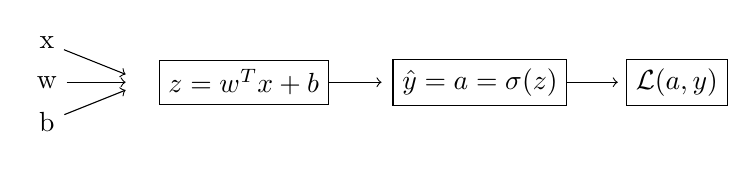
\begin{tikzpicture}
  \node (x) at (0, 1) {x};
  \node (w) at (0,.5) {w};
  \node (b) at (0, 0) {b};
  \draw[->] (x) to (1, .6);
  \draw[->] (w) to (1, .5);
  \draw[->] (b) to (1, .4);
  \node[draw=black,rectangle] (z) at (2.5, .5) {$z = w^Tx + b$};
  \draw[->] (z) to (4.25, .5);
  \node[draw=black,rectangle] (yhat) at (5.5, .5) {$\hat y = a = \sigma(z)$};
  \draw[->] (yhat) to (7.25, .5);
  \node[draw=black,rectangle] (loss) at (8, .5) {$\mathcal L (a,y)$};
\end{tikzpicture}
\end{center} We seek to learn $w, b$ to minimize the loss function. \emph{Back propogation} proceeds as follows:

{
\small{
\begin{align*}
\texttt{da} &= \frac{\partial \mathcal L}{\partial a} = - \left(\frac{y}{a} - \frac{1-y}{1-a}\right) = \frac{-y}{a} + \frac{1-y}{1-a}. \\
  \texttt{dz} &= \frac{\partial \mathcal L}{\partial z} = \frac{\partial \mathcal L}{\partial a}\frac{\partial a}{\partial z} = \left(\frac{-y}{a} + \frac{1-y}{1-a}\right) \times a(1-a) = \frac{-y}{a} \cdot a(1-a) + \frac{1-y}{1-a} \cdot (1-a) a = -y(1-a)+ (1-y)a \\ &= ay - y + a - ay = a - y.  \\
\texttt{dw} &= \frac{\partial \mathcal L}{\partial w} \overset{?}{=} \frac{\partial \mathcal L}{\partial z} \frac{\partial z}{\partial w} = (a-y) x^T. \\
\texttt{db} &= \frac{\partial \mathcal L}{\partial b} = \frac{\partial \mathcal L}{\partial z} \underbrace{\frac{\partial z}{\partial b}}_{=1}. \end{align*}
}
}
Our update rule then becomes: $w := w - \alpha \texttt{dw}$, and $b := b - \alpha \texttt{db}$. Our (average) \emph{cost} function is defined as $J(w,b) = \frac{1}{m} \sum_{i=1}^m \mathcal L(a^{(i)}, y^{(i)})$. Since $\frac{\partial}{\partial \cdot}$ is a linear operator, obtaining gradients is quite straightforward since we are left with a series of derivatives of loss functions, which we calculated above.
\begin{align*}    \frac{\partial J}{\partial w} = \frac{1}{m} \sum \frac{\partial \mathcal L}{\partial w}, \hspace{15pt} \textrm{and} \hspace{15pt} \frac{\partial J}{\partial b} = \frac{1}{m} \sum \frac{\partial \mathcal L}{\partial b} \end{align*}
Our optimization routine then can be written as in algorithm \ref{alg: logisticreg}

{\small
\begin{algorithm}[H]
  \label{alg: logisticreg}
  \caption{Logistic Regression - Optimization}   \For{\texttt{i in range(m)}} {
    $z^{(i)} = w^Tx^{(i)} + b$ \\
    $a^{(i)} = \sigma(z^{(i)})$ \\
    $J += - \left[ y^{(i)} \log a^{(i)} + (1-y^{(i)}) \log (1 - a^{(i)}) \right]$ \\
    $\partial d z^{(i)} = a^{(i)} - y^{(i)}$ \\
    $\partial d w += \partial d z^{(i)} {x^{(i)}}^T$ \\
    $\partial d b += \partial d z^{(i)}$
}
$J /= m$ \\
$\partial w /= m$ \\
$\partial b /= m$ \end{algorithm}
}
The above concludes one round of \href{https://en.wikipedia.org/wiki/Gradient_descent}{Gradient Descent}. We repeat this procedure many times until training loss (and ideally test loss ) is sufficiently minimized. We remark that it's possible to remove both \texttt{for} loops (over the training data, and over the parameters in $w$) by using vectorized operations in \texttt{numpy}. We execute this in code \href{https://github.com/asantucci/NN/blob/master/logistic_regression.py#L46}{here}.

\section{Neural Networks with 2-layers}
\vspace{-10pt}
We previously saw a simple computation graph. 
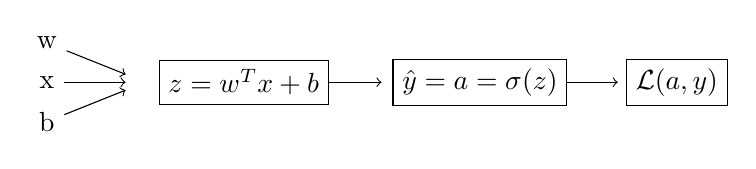
\begin{tikzpicture}   \node (w) at (0, 1) {w};
  \node (x) at (0, .5) {x};
  \node (b) at (0,0) {b};
  \draw[->] (x) to (1, .5);
  \draw[->] (w) to (1, .6);
  \draw[->] (b) to (1, .4);
  \node[draw=black,rectangle] (z) at (2.5, .5) {$z = w^Tx + b$};
  \draw[->] (z) to (4.25, .5);
  \node[draw=black,rectangle] (yhat) at (5.5, .5) {$\hat y = a = \sigma(z)$};
  \draw[->] (yhat) to (7.25, .5);
  \node[draw=black,rectangle] (loss) at (8, .5) {$\mathcal L (a,y)$};
\end{tikzpicture}
\subsection{Understanding Small Neural Networks}
A Neural Network can be constructed by stacking together sigmoids, depicted as follows:
\begin{figure}[h]
\centering
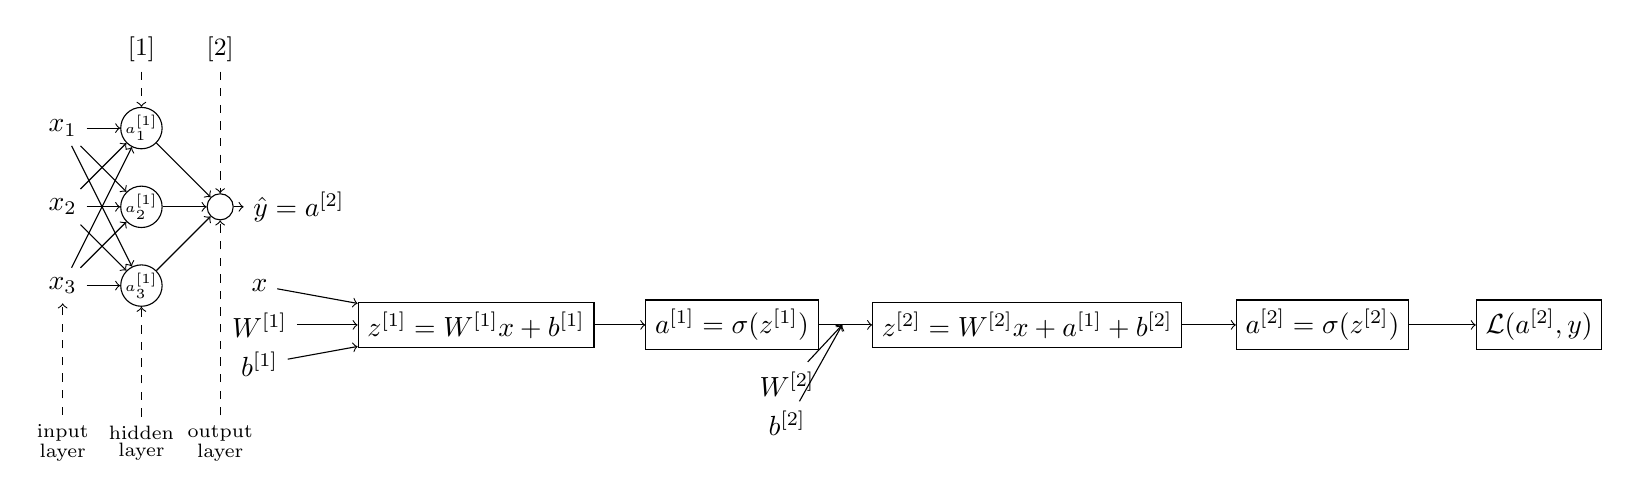
\begin{tikzpicture}
  \node (x1) at (0, 1) {$x_1$};
  \node (x2) at (0, 0) {$x_2$};
  \node (x3) at (0,-1) {$x_3$};
  \node (inputlayer) at (0, -3) {$\substack{\textrm{input}\\ \textrm{layer}}$};
  \draw[->,dashed] (inputlayer) to (x3);
  \node (lbl) at (1,2) {\small{$[1]$}}; 
  \node[draw=black,circle,inner sep = 0pt] (n1) at (1, 1) {\tiny $a_1^{[1]}$};
  \draw[->,dashed] (lbl) to (n1);
  \node[draw=black,circle,inner sep = 0pt] (n2) at (1, 0) {\tiny $a_2^{[1]}$};
  \node[draw=black,circle,inner sep = 0pt] (n3) at (1,-1) {\tiny $a_3^{[1]}$};
  \node (hiddenlayer) at (1, -3) {$\substack{\textrm{hidden}\\ \textrm{layer}}$};
  \draw[->,dashed] (hiddenlayer) to (n3);
  \draw[->] (x1) to (n1);
  \draw[->] (x1) to (n2);
  \draw[->] (x1) to (n3);   \draw[->] (x2) to (n1);
  \draw[->] (x2) to (n2);
  \draw[->] (x2) to (n3);   
  \draw[->] (x3) to (n1);
  \draw[->] (x3) to (n2);
  \draw[->] (x3) to (n3); 
  \node[draw=black,circle] (m1) at (2,0) {};
  \node (lbl2) at (2,2) {\small{$[2]$}}; 
  \draw[->,dashed] (lbl2) to (m1);
  \node (yhat) at (3,0) {$\hat y = a^{[2]}$};
  \node (outputlayer) at (2, -3) {$\substack{\textrm{output}  \\ \textrm{layer}}$};
  \draw[->,dashed] (outputlayer) to (m1);
  \draw[->] (n1) to (m1);
  \draw[->] (n2) to (m1);
  \draw[->] (n3) to (m1);
  \draw[->] (m1) to (yhat);
  \node (x) at (2.5, -1) {$x$};
  \node (w1) at (2.5, -1.5) {$W^{[1]}$};
  \node (b1) at (2.5, -2) {$b^{[1]}$};
  \node[draw=black,rectangle] (z1) at (5.25, -1.5) {$z^{[1]} = W^{[1]}x + b^{[1]}$};
  \draw[->] (x) to (z1);
  \draw[->] (w1) to (z1);
  \draw[->] (b1) to (z1);
  \node[draw=black,rectangle] (a1) at (8.5, -1.5) {$a^{[1]} = \sigma (z^{[1]})$};
  \draw[->] (z1) to (a1);
  \node[draw=black,rectangle] (z2) at (12.25, -1.5) {$z^{[2]} = W^{[2]}x + a^{[1]} + b^{[2]}$};
  \draw[->] (a1) to (z2);
  \node (w2) at (9.2, -2.25) {$W^{[2]}$};
  \node (b2) at (9.2, -2.75) {$b^{[2]}$};
  \draw[->] (w2) to (9.9, -1.5);
  \draw[->] (b2) to (9.9, -1.5);
  \node[draw=black,rectangle] (a2) at (16, -1.5) {$a^{[2]} = \sigma(z^{[2]})$};
  \draw[->] (z2) to (a2);
  \node[draw=black,rectangle] (l) at (18.75, -1.5) {$\mathcal L(a^{[2]},y)$};
  \draw[->] (a2) to (l);
\end{tikzpicture}
\caption{A 2-layer Neural Network (you could say we don't count the input layer, or you could say we do but we index starting from zero).}
\end{figure}
\newline
\vspace{-40pt}
\paragraph{Terminology and Notation}
Each \emph{neuron} in the graph consists of both a linear transformation and a non-linear activation function, i.e. the first stack of nodes will produce a $z$ and an $a$. We use the super-script square brackets $[\hspace{2pt} ]$ to denote a stack of nodes, i.e. a layer, not to be confused with super-script parentheses which index training examples. I.e. $a^{[\ell]}_i$ denotes the output of an activation function in layer $\ell$ for the $i$th neuron.
The key difference between our Logistic Regression and 
this (or any) Neural Network is that we simply repeat linear transformations followed by non-linear activation functions \emph{multiple times}.
The reason why we call the intermediary layer a ``hidden'' layer is because we do not observe what these values are to be in the training set. By convention, we define  $a^{[0]} = X$. We can further refer to the hidden layer by ${a^{[1]}} = \begin{bmatrix}   a_1^{[1]} & a_2^{[1]} & a_3^{[1]}  \end{bmatrix}^T$. Notice that the hidden layer and output layer have parameters $W^{[\cdot]}$ and $b^{[\cdot]}$ associated with them. 

\paragraph{Visualizing a Neuron}
Let's take a look at neural network representation in a bit more detail. We can think about each neuron as being divided into two parts: one which performs a linear transformation and another which performs an activation function. The mental model is:
\begin{figure}[h]
  \centering   
  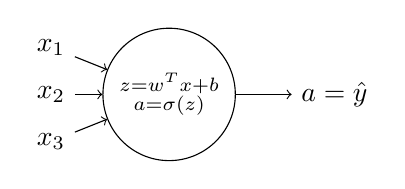
\begin{tikzpicture}[scale=0.6]     
    \node (x1) at (-1, 1) {$x_1$};
    \node (x2) at (-1, 0) {$x_2$};
    \node (x3) at (-1,-1) {$x_3$};
    \node[draw,circle] (neuron) at (1.5,0) {$\substack{z = w^Tx + b \\ a = \sigma(z)}$};
    \draw[->] (x1) to (neuron);
    \draw[->] (x2) to (neuron);
    \draw[->] (x3) to (neuron);
    \node (output) at (5,0) {$a = \hat y$};
    \draw[->] (neuron) to (output);
  \end{tikzpicture} \end{figure}
\newline
In general, we'll have something as follows for the first neuron in the hidden layer, and to be crystal clear we draw out the second neuron as well.
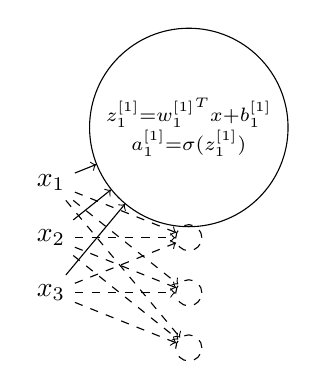
\begin{tikzpicture}[scale=0.7]     
  \node (x1) at (0, 1) {$x_1$};
    \node (x2) at (0, 0) {$x_2$};
    \node (x3) at (0,-1) {$x_3$};
    \node[draw,circle] (neuron) at (2.5,2) {$\substack{z_1^{[1]} = {w_1^{[1]}}^Tx + b_1^{[1]} \\ a_1^{[1]} = \sigma(z_1^{[1]})}$};
    \draw[->] (x1) to (neuron);
    \draw[->] (x2) to (neuron);
    \draw[->] (x3) to (neuron);
    \node[draw,circle,dashed] (n2) at (2.5,0 ) {};     \node[draw,circle,dashed] (n3) at (2.5,-1) {}; 
    \node[draw,circle,dashed] (n4) at (2.5,-2) {}; 
    \draw[->,dashed] (x1) to (n2);
    \draw[->,dashed] (x2) to (n2);
    \draw[->,dashed] (x3) to (n2);
    \draw[->,dashed] (x1) to (n3);
    \draw[->,dashed] (x2) to (n3);
    \draw[->,dashed] (x3) to (n3);
    \draw[->,dashed] (x1) to (n4);
    \draw[->,dashed] (x2) to (n4);
    \draw[->,dashed] (x3) to (n4);
\end{tikzpicture}
\hspace{20pt} 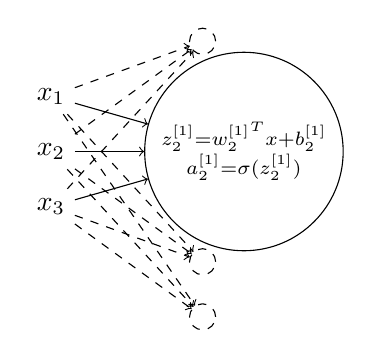
\begin{tikzpicture}[scale=0.7]     
    \node (x1) at (0, 1) {$x_1$};
    \node (x2) at (0, 0) {$x_2$};
    \node (x3) at (0,-1) {$x_3$};
    \node[draw,circle,dashed] (neuron) at (2.75,2) {};
    \draw[->,dashed] (x1) to (neuron);
    \draw[->,dashed] (x2) to (neuron);
    \draw[->,dashed] (x3) to (neuron);
    \node[draw,circle] (n2) at (3.5,0 ) {$\substack{z_2^{[1]} = {w_2^{[1]}}^Tx + b_2^{[1]} \\ a_2^{[1]} = \sigma(z_2^{[1]})}$};     
    \node[draw,circle,dashed] (n3) at (2.75,-2) {}; 
    \node[draw,circle,dashed] (n4) at (2.75,-3) {}; 
    \draw[->] (x1) to (n2);
    \draw[->] (x2) to (n2);
    \draw[->] (x3) to (n2);
    \draw[->,dashed] (x1) to (n3);
    \draw[->,dashed] (x2) to (n3);
    \draw[->,dashed] (x3) to (n3);
    \draw[->,dashed] (x1) to (n4);
    \draw[->,dashed] (x2) to (n4);
    \draw[->,dashed] (x3) to (n4);
\end{tikzpicture} 
To avoid having to calculate $z_i^{[\ell]}$ using a \texttt{for}
loop, we can instead use a matrix multiply, where $W^{[1]} \in \mathbb R^{n_1, n_x}$:
$$
W^{[1]}x + b^{[1]} = 
\underbrace{\begin{bmatrix}    & {w_1^{[1]}}^T & \\
   & {w_2^{[1]}}^T & \\    & {w_3^{[1]}}^T & \\    
   & {w_4^{[1]}}^T & \\ 
\end{bmatrix}}_{\in \mathbb R^{4, 3}} \begin{bmatrix} x_1 \\ x_2 \\ x_3  \end{bmatrix} + \begin{bmatrix}   b_1^{[1]} \\ b_2^{[1]} \\ b_3^{[1]} \\ b_4^{[1]} \end{bmatrix} = \begin{bmatrix}   z_1^{[1]} \\
  z_2^{[1]} \\
  z_3^{[1]} \\
  z_4^{[1]} \\ \end{bmatrix} = z^{[1]}
$$
We can then write ${a^{[1]}}^T = \begin{bmatrix}   a_1^{[1]} & a_2^{[1]} & a_3^{[1]} & a_4^{[1]} \end{bmatrix} = \sigma (z^{[1]})$ where the $\sigma(\cdot)$ is applied element-wise.
Given an input $x$, we set $a^{[0]} = x$ and we compute forward steps: $z^{[\ell]} = W^{[\ell]}a^{[\ell-1]} + b^{[\ell]}$
for each layer in the network.

\paragraph{Vectorization} Suppose we have a single hidden-layer neural network. As per above, the forward propagation involves computing: 
$  z^{[1]} = W^{[1]}a^{[0]} + b^{[1]}; \hspace{10pt} a^{[1]} = \sigma(z^{[1]}); \hspace{10pt} 
   z^{[2]} = W^{[2]}a^{[1]} + b^{[2]}; \hspace{10pt} 
   a^{[2]} = \sigma(z^{[2]}).
$
We need to replicate this procedure for each of our $m$ training samples. I.e. we need to feed each training example through the network to get an output. Let our final output be denoted by $a^{[\ell](j)}$ denote the output for the activation function for the $j$th training example at the $\ell$th layer in our network. So in our case above, $a^{[2](j)}$ is the output for the $j$th training example.
We'd like to avoid applying a \texttt{for} loop over each of our $m$ training examples, like so:
{\footnotesize
\begin{algorithm}[h]
  \caption{Naive Forward Propagation on a 2-layer Neural Network}   \For{i = 1 to m}{
    $z^{[1](i)} = W^{[1]}x^{(i)} + b^{[1]}$ \\
    $a^{[1](i)} = \sigma(z^{[1]}(i))$ \\
    $z^{[2](i)} = W^{[2]}a^{[1](i)} + b^{[2]}$ \\
    $a^{[2](i)} = \sigma(z^{[2]}(i))$
  } \end{algorithm}
}
\newline
\vspace{-.5ex}Recall we arranged our input matrix such that each column is an observation, i.e. $X = \begin{bmatrix}    | & | & & | \\    x^{(1)} & x^{(2)} & \ldots & x^{(m)} \\   | & | & & |  \end{bmatrix} \in \mathbb R^{n_x, m}$. Then,
$  
  Z^{[1]} = W^{[1]} X + b^{[1]}; \hspace{10pt}
  A^{[1]} = \sigma(Z^{[1]}); \hspace{10pt}
  Z^{[2]} = W^{[2]} A^{[1]} + b^{[2]}; \hspace{10pt}
  A^{[2]} = \sigma(Z^{[2]})
$ To be explicit, $Z^{[1]}$ is also arranged with observations in columns, i.e. $Z^{[1]} = \begin{bmatrix}   | & | & & | \\ z^{[1](1)} & z^{[1](2)} & \ldots & z^{[1](m)} \\ | & | & & | \end{bmatrix}$ and $A^{[1]} = \begin{bmatrix}    | & | & & | \\    a^{[1](1)} & a^{[1](2)} & \ldots & a^{[1](m)}  \\  | & | & & | \end{bmatrix}$.\footnote{As one scans matrix $A^{[\ell]}$ from left to right, we scan through observations or training examples, and as we scan from top to bottom we scan through the activations of different hidden units.}

\subsection{Activation Functions}
\paragraph{Hyperbolic Tangent}
Another activation function to consider is $\tanh (z) = \frac{e^z - e^{-z}}{e^z + e^{-z}}$. It's a shifted and rescaled version of the sigmoid function, which ranges from $[-1, 1]$ and cross the $x$-axis at zero; it is intuitively thought to perform better than a sigmoid activation function since it has the effect of ``centering'' the data in the intermediate layers of the network around zero. The one exception is the output layer: if we are predicting binary classification it makes sense to use sigmoid since our target values are in $\{0, 1\}$ we therefore want $\hat y$ to be in $(0,1)$.

\begin{figure}[h]
  \centering   
  \begin{tikzpicture}[scale=0.7]   \draw[->] (-3,0) -- (3,0) node[right] {$x$};   \draw[->] (0,-1) -- (0,1) node[above] {$y$};
  \draw[domain=-3:3,smooth,variable=\x,blue] plot ({\x},{(exp(\x) - exp(-\x))/(exp(\x) + exp(-\x))}); 
\end{tikzpicture}   \end{figure}
Both sigmoid and $\tanh$ suffer from the problem of saturating gradients. I.e. if the input value is either very small or very large, the derivative of the function becomes very small. This has the effect of slowing down gradient descent.

\paragraph{Rectified Linear Unit}
This leads us to the rectified linear unit: $a = g(z) = \max\{0, z\}$. The derivative at zero is not well defined, however, it is unlikely that we will ever encounter a true zero in our computations and so we can ignore this case without much worry. One disadvantage of the ReLU is that its derivative is identically zero when the input is negative, but this ends up not harming us in practice: enough neurons will likely have positive inputs such that gradients can still be learned. There is also the leaky ReLU: $a = g(z) = \max\{0.01 \times z, z\}$.

\begin{figure}[h]
  \centering   
  \begin{tikzpicture}[scale=1.2]
    \draw[->] (-1,0) -- (1,0) node[right] {$x$};   
    \draw[->] (0,-1) -- (0,1) node[above] {$y$};
    \draw[domain=-1:1,smooth,variable=\x,blue] plot ({\x},{max(0,\x)}); 
  \end{tikzpicture}   
\end{figure}

\paragraph{Linear Activation Function (Identity Function)} It's worthwhile to realize that if we only used linear activation functions $g(z) = z$, then our neural network would in fact be a linear model. This is easy to see, since if $a^{[1]} = z^{[1]} = W^{[1]} x + b^{[1]}$ and $z^{[2]} = W^{[2]} a^{[1]} + b^{[2]}$ then plugging in for $a^{[1]}$, $z^{[2]} = W^{[2]} (W^{[1]} x + b^{[1]}) + b^{[2]} = \underbrace{W^{[2]}W^{[1]}}_{=W'}x + \underbrace{W^{[2]}b^{[1]} + b^{[2]}}_{b'}$ which is linear with respect to the input $x$. The one time we may use a linear activation function is if, for example, we were predicting housing prices, in which case we may want our output to range arbitrarily high. Even then, a better choice would be ReLU since housing prices are non-negative.

\subsubsection{Derivatives of Activation Functions} 
\paragraph{Hyperbolic Tangent}
Recall that 
\begin{align*}   \sinh(x) = \frac{e^x - e^{-x}}{2}, \hspace{10pt} 
  \cosh(x) = \frac{e^x + e^{-x}}{2}, \hspace{10pt} \textrm{ and } \hspace{5pt}
  \tanh(x) = \frac{\sinh(x)}{\cosh(x)}. \end{align*}
It's easy to see using linearity of $\frac{\d \,}{\d x}$ and the chain rule that $\frac{\d \,}{\d x}  \sinh(x) = \frac{e^x}{2} + \frac{e^{-x}}{2} = \cosh(x)$ and similarly that $\frac{\d \,}{\d x}\cosh(x) = \sinh(x)$. Then, apply either quotient rule \emph{or} both the product rule and chain rule:
\begin{align*}   \frac{\d \,}{\d x} \tanh(x) = \frac{\d \,}{\d x} \sinh(x) \cosh(x)^{-1} = \cosh(x) \cosh(x)^{-1} - \sinh(x)\cosh(x)^{-2}\sinh(x) = 1 - \tanh(x)^2. \end{align*}
\paragraph{Rectified Linear Unit} has derivative equal to
\begin{align}   \frac{\d \,}{\d x} \max\{0,x\}=       \begin{cases}        0 &\quad\text{if } x < 0\\        1 &\quad\text{if } x > 0 \\
       \textrm{undefined} &\quad\text{if } x = 0      \end{cases} \end{align}
Technically the derivative is undefined when $x = 0$, however, in practice a floating point variable never takes on the value zero exactly. We can therefore ignore this case by choosing to ``define'' the gradient to be either zero or one (which we choose again doesn't matter in practice). Either way, note that ReLU is convex and so we realize a \href{https://en.wikipedia.org/wiki/Subderivative}{sub-derivative}.

\paragraph{Leaky ReLU} is defined as $\max \{0.01 x, x \}$ and its derivative is therefore given by
\begin{align}   
  \frac{\d \,}{\d x} \max\{0.01x,x\}=       
  \begin{cases}        
    0.01 &\quad\text{if } x < 0\\        
    1    &\quad\text{if } x > 0 \\
    \textrm{undefined} &\quad\text{if } x = 0      
  \end{cases} 
\end{align}
Again the fact that the derivative doesn't exist at $x=0$ doesn't matter in practice since we're dealing with floating point values that are never identically zero.

\subsection{Back-Propagation for Neural Networks}
\paragraph{Review: Logistic Regression Computation Graph}
Recall our logistic regression computation graph. After computing our forward pass, we needed to compute a backward pass by calculating gradients at each step, depicted in \color{orange}{orange} \color{black} below.
\begin{figure}[h]
\centering 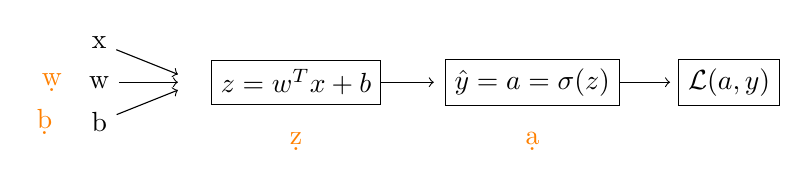
\begin{tikzpicture}
  \node (x) at (0, 1) {x};
  \node (w) at (0, .5) {w};
  \node (b) at (0,0) {b};
  \node [left = .1cm of w] {\color{orange}$\d w$}; 
  \node [left = .25cm of b] {\color{orange}$\d b$}; 
  \draw[->] (x) to (1, .6);
  \draw[->] (w) to (1, .5);
  \draw[->] (b) to (1, .4);
  \node[draw=black,rectangle] (z) at (2.5, .5) {$z = w^Tx + b$};
  \node at (2.5,-0.25) {\color{orange}$\d z$};
  \draw[->] (z) to (4.25, .5);
  \node[draw=black,rectangle] (yhat) at (5.5, .5) {$\hat y = a = \sigma(z)$};
  \node at (5.5,-0.25) {\color{orange}$\d a$};
  \draw[->] (yhat) to (7.25, .5);
  \node[draw=black,rectangle] (loss) at (8, .5) {$\mathcal L (a,y)$};
\end{tikzpicture}   \end{figure}
\newline
Note that $\d z = \d a \cdot g'(z)$ where $g(z) = \sigma(z)$, i.e. we use the fact that $\frac{\d L(a,y)}{\d z} = \frac{\d L(a,y)}{\d a} \frac{\d a}{\d z}$.

\paragraph{Two Layer Neural Network Back Propagation}
Let us now reconsider our two layer neural network and 
its computation graph. We highlight terms we must compute in \color{orange}{orange}\color{black}.
\begin{figure}[h]
\hspace{-20pt}
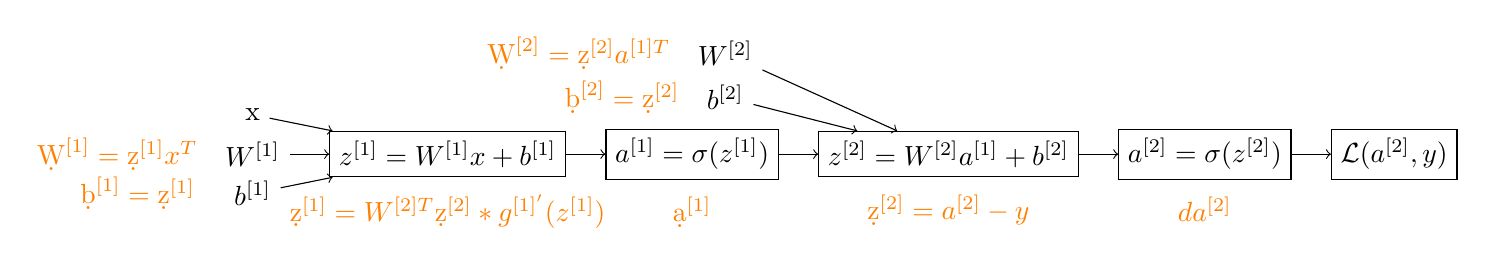
\begin{tikzpicture}
  \node (x)  at (-3, 1)  {x};
  \node (w1) at (-3, .5) {$W^{[1]}$};
  \node (b1) at (-3,0)   {$b^{[1]}$};
  \node [left = .1cm of w1] {\color{orange}$\d W^{[1]}= \d z^{[1]} x^T$}; 
  \node [left = .25cm of b1] {\color{orange}$\d b^{[1]}= \d z^{[1]}$}; 
  \node[draw=black,rectangle, right = .5cm of w1] (z1)  {$z^{[1]} = W^{[1]}x + b^{[1]}$};
  \draw[->] (x) to (z1);
  \draw[->] (w1) to (z1);
  \draw[->] (b1) to (z1);
  \node [below = .1cm of z1] {\color{orange}$\d z^{[1]}=W^{[2]T} \d z^{[2]} * g^{[1]'}(z^{[1]})$};
  \node[draw=black,rectangle, right = .5cm of z1] (a1) {$a^{[1]} = \sigma(z^{[1]})$};
  \draw[->] (z1) to (a1);
  \node [below = .1cm of a1] {\color{orange}$\d a^{[1]}$};
  \node[draw=black,rectangle, right = .5cm of a1] (z2) {$z^{[2]} = W^{[2]} a^{[1]} + b^{[2]}$};
  \node[below=.1cm of z2] (dz2) {\color{orange} $\d z^{[2]}= a^{[2]} - y$};
  \draw[->] (a1) to (z2);
  \node[above left = 1cm of z2] (w2) {$W^{[2]}$};
  \node[left = .1cm of w2] (dw2) {\color{orange}$\d W^{[2]}= \d z^{[2]} a^{[1]T}$};
  \node[below = .00025cm of w2] (b2) {$b^{[2]}$};
  \node[left = .1cm of b2] (db2) {\color{orange}$\d b^{[2]} = \d z^{[2]}$};
  \draw[->] (w2) to (z2);
  \draw[->] (b2) to (z2);
  \node[draw=black,rectangle,right = .5cm of z2] (a2) {$a^{[2]} = \sigma(z^{[2]})$};
  \node[below=.1cm of a2] (da2) {\color{orange} $da^{[2]}$};
  \draw[->] (z2) to (a2);
  \node[draw=black,rectangle,right=.5cm of a2] (loss) {$\mathcal{L}(a^{[2]}, y)$};
  \draw[->] (a2) to (loss);
\end{tikzpicture}   
\end{figure}
\newline
Where in $\d z^{[1]}=W^{[2]T} \d z^{[2]} * g^{[1]'}(z^{[1]})$ the $*$ denotes an element-wise product.
Note that the computations for $\d a^{[\ell]}$ are typically rolled into the next computation for $\d z^{[\ell]}$.
Further realize that the above computations are performed for \emph{each} training example in our data set 
during gradient descent.
\paragraph{Vectorized Implementation}
We can vectorize our computations as follows.
\begin{align*}   \d Z^{[2]} &= A^{[2]} - Y \\
  \d W^{[2]} &= \frac{1}{m} \d Z^{[2]} {A^{[1]}}^T \\
  \d b^{[2]} &= \frac{1}{m} \texttt{np.sum}(\d Z^{[2]}\texttt{, axis = 1, keepdims = True}) \\
  \d Z^{[1]} &= {W^{[2]}}^T \d Z^{[2]} * g^{[1]'}(Z^{[1]}) \hspace{35pt} (* \textrm{ denotes an element-wise product})\\
  \d W^{[1]} &= \frac{1}{m} \d Z^{[1]} X^T \\ 
  \d b^{[1]} &= \frac{1}{m} \texttt{np.sum}(\d Z^{[1]}\texttt{, axis = 1, keepdims = True}) \end{align*}

\subsubsection{Random Initialization}
\paragraph{Why Initializing With Zeros Won't Work for $W$'s: Symmetric Neurons}
Note that initializing our weights matrix with zeros will prevent gradient descent from working. What happens? For any example, $a_1^{[1]} = a_2^{[2]}$, whence $\d z_1^{[1]} = \d z_2^{[2]}$. I.e. the hidden units are symmetrical, and $\d W = \begin{bmatrix}   u & v \\ u & v \end{bmatrix}$ and our weights matrix will have first row equal to the second row. By induction, no matter how many times we train our network, the neurons in the hidden layer will remain symmetric and no learning will take place. 
It turns out $b$ does not have this symmetry-breaking problem, and so we can initialize $b$'s to zeros.

\paragraph{Random Initialization}
Instead, if we initialize weights randomly, each neuron in each hidden layer will compute different functions. I.e. $W^{[1]} = $\texttt{np.random.randn((.,.)) * 0.01} where we apply an ad-hoc scaling factor. We prefer initializing weights to small values. Why? Suppose we are using either sigmoid or $\tanh$ activation functions then if $W$ initialized large, $Wx + b$ also large, whence $g(z)$ large and we yield saturated (near-zero) gradients; this means gradient descent and learning will be very slow. If we don't have any sigmoid or $\tanh$ activation functions, this is less of an issue. 

\section{Deep Learning: $L$-layer Neural Networks}

Let's consider a four layer neural network, depicted below in figure \ref{fig: fourlayernet}.
Let us define some notation. Let $L=4$ denote the number of layers in the network. The notation $n^{[\ell]} = \# \textrm{units in layer } \ell$.

\begin{figure}[h]   \centering
  \label{fig: fourlayernet}
  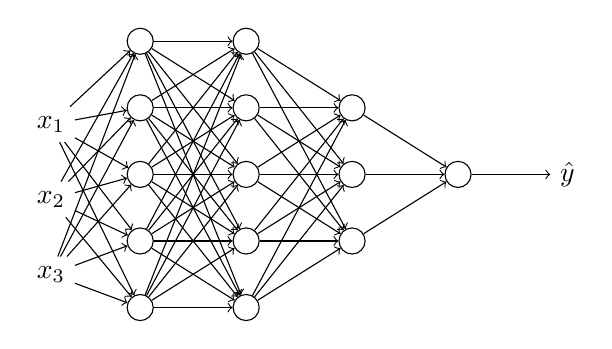
\begin{tikzpicture}[scale=0.25]     \node (x1) at (-2, 1) {$x_1$};
    \node [below = .5 cm of x1] (x2) {$x_2$};
    \node [below = .5 cm of x2] (x3) {$x_3$};
    \node [draw,circle,above right = 1 cm of x1] (n11) {};
    \node [draw,circle,below = .5 cm of n11] (n12) {};
    \node [draw,circle,below = .5cm of n12] (n13) {};
    \node [draw,circle,below = .5cm of n13] (n14) {};
    \node [draw,circle,below = .5cm of n14] (n15) {};
    \node [draw,circle,right = 1 cm of n11] (n21) {};
    \node [draw,circle,below = .5 cm of n21] (n22) {};
    \node [draw,circle,below = .5cm of n22] (n23) {};
    \node [draw,circle,below = .5cm of n23] (n24) {};
    \node [draw,circle,below = .5cm of n24] (n25) {};
    \node [draw,circle,right = 1cm of n22] (n31) {};
    \node [draw,circle,below = .5cm of n31] (n32) {};
    \node [draw,circle,below = .5cm of n32] (n33) {};
    \node [draw,circle,right = 1cm of n32] (outputneuron) {};
    \node [right = 1cm of outputneuron] (yhat) {$\hat y$};
    \draw[->] (x1) to (n11);
    \draw[->] (x1) to (n12);
    \draw[->] (x1) to (n13);
    \draw[->] (x1) to (n14);
    \draw[->] (x1) to (n15);
    \draw[->] (x2) to (n11);
    \draw[->] (x2) to (n12);
    \draw[->] (x2) to (n13);
    \draw[->] (x2) to (n14);
    \draw[->] (x2) to (n15);
    \draw[->] (x3) to (n11);
    \draw[->] (x3) to (n12);
    \draw[->] (x3) to (n13);
    \draw[->] (x3) to (n14);
    \draw[->] (x3) to (n15);
    \draw[->] (n11) to (n21);
    \draw[->] (n11) to (n22);
    \draw[->] (n11) to (n23);
    \draw[->] (n11) to (n24);
    \draw[->] (n11) to (n25);
    \draw[->] (n12) to (n21);
    \draw[->] (n12) to (n22);
    \draw[->] (n12) to (n23);
    \draw[->] (n12) to (n24);
    \draw[->] (n12) to (n25);
    \draw[->] (n13) to (n21);
    \draw[->] (n13) to (n22);
    \draw[->] (n13) to (n23);
    \draw[->] (n13) to (n24);
    \draw[->] (n13) to (n25);
    \draw[->] (n14) to (n21);
    \draw[->] (n14) to (n22);
    \draw[->] (n14) to (n23);
    \draw[->] (n14) to (n24);
    \draw[->] (n14) to (n25);
    \draw[->] (n15) to (n21);
    \draw[->] (n15) to (n22);
    \draw[->] (n15) to (n23);
    \draw[->] (n15) to (n24);
    \draw[->] (n15) to (n25);
    \draw[->] (n21) to (n31);
    \draw[->] (n21) to (n32);
    \draw[->] (n21) to (n33);
    \draw[->] (n22) to (n31);
    \draw[->] (n22) to (n32);
    \draw[->] (n22) to (n33);
    \draw[->] (n23) to (n31);
    \draw[->] (n23) to (n32);
    \draw[->] (n23) to (n33);
    \draw[->] (n24) to (n31);
    \draw[->] (n24) to (n32);
    \draw[->] (n24) to (n33);
    \draw[->] (n25) to (n31);
    \draw[->] (n25) to (n32);
    \draw[->] (n25) to (n33);
    \draw[->] (n31) to (outputneuron);
    \draw[->] (n32) to (outputneuron);
    \draw[->] (n33) to (outputneuron);
    \draw[->] (outputneuron) to (yhat);
  \end{tikzpicture}
  \caption{Four-layer, fully connected neural network.} \end{figure}
In our example depicted, $n^{[0]} = n_x = 3$, $n^{[1]} = n^{[2]} = 5$ and $n^{[3]} = 3$ and $n^{L} = 1$. We'll also use $a^{[\ell]} = g^{[\ell]}(z^{[\ell]})$ to denote the activations in layer $\ell$, where to compute $z^{[\ell]}$ we use weights matrix $W^{[\ell]}$ and bias term $b^{[\ell]}$. Lastly, realize that with this notation our input matrix $X = a^{[0]}$ and our output $\hat y = a^{[L]}$.

\paragraph{Forward Propagation}
In general, we have that for a single training example:
\begin{align*}   z^{[\ell]} &= W^{[\ell]} a^{[\ell-1]} + b^{[\ell]}, \\ 
  a^{[\ell]} &= g^{[\ell]}(z^{[\ell]}). \end{align*}
And for our entire training set, where $X = A^{[0]}$ is our data arranged such that each column is an observation:
\begin{align*}   Z^{[\ell]} &= W^{[\ell]} A^{[\ell-1]} + b^{[\ell]}, \\ 
  A^{[\ell]} &= g^{[\ell]}(Z^{[\ell]}).    \end{align*}
Note that by rules of matrix multiplication, it's easy to see that $Z^{[\ell]}$ must have as many columns as there are training examples, and since $g^{[\ell]}$ is applied element-wise then $A^{[\ell]}$ also has as $m$ columns.
For our last layer, $\hat Y = g(Z^{[L]}) = A^{[L]}$. We remark that although we typically try to vectorize code and remove \texttt{for}-loops, it is perfectly reasonable to loop over the layers in the network during forward propagation. I.e. we expect to see \texttt{for} $\ell = 1, \ldots, L$.

\paragraph{Getting Your Dimensions Right} In general, the dimension for a weights matrix at layer $\ell$ is given b
\begin{equation}   W^{[\ell]} : \left( n^{[\ell]}, n^{[\ell - 1]} \right). \end{equation}
What about our bias term? In general, $b^{[\ell]} : \left(n^{[\ell]}, 1\right)$, Further, during backpropogation, the dimensions of the derivative matrices don't change. I.e. 
$\d   W^{[\ell]} : \left( n^{[\ell]}, n^{[\ell - 1]} \right)$, and $\d b^{[\ell]} : \left(n^{[\ell]}, 1\right)$.

\paragraph{Deep Representations:
\small What do our intermediary layers come to learn in different applications?}
\begin{itemize} \item Consider face detection. The first layer of the network may learn to detect edges, and the second layer perhaps may learn how to detect different pieces of a face by connecting edges together such as an eye or an ear. A later layer of a network may learn to distinguish between faces at an even less granular level.

\item As another example consider problems in the context of audio. The first layer of the network may lrn to distinguish between low and high frequency waveforms, whereas the second layer may learn to recognize phonemes (in the word cat, each letter, when pronounced, is a phoneme), and later layers of the network may learn to recognize words and finally phrases/sentences.
\end{itemize}
Earlier layers are in general based on more granular features, i.e. simple transformations of the input data. Later layers compose hierarchically and are eventually able to solve complex tasks.   
\paragraph{Circuit Theory and Deep Learning}
``There are functions you can compute with a `small' $L$-layer deep neural network that shallower networks require exponentially more hidden units to compute.''

As an example, consider using a neural network to approximate \texttt{xor} applied to $n$ input bits. I.e. we seek to calculate $x_1 \textrm{ xor } x_2 \textrm{ xor } \ldots \textrm{ xor } x_n$. If we are free to use as many layers in the network as we wish, then we could envision building a \texttt{xor} tree as follows: pair successive inputs together and apply the \texttt{xor} operation, and pipe the resulting output into the subsequent layer of the network. Realize that we require $\log n$ layers in our network in order to exactly compute the right answer. If, on the other hand, we weren't allowed to use an arbitrary number of layers but instead only a single hidden layer, we would require $O(2^n)$ neurons in order to achieve the same result; to see why realize that we effectively need to enumerate all possible $2^n$ possible input sequences in order to map them correctly back to the right answer in a subsequent step. Note that it is possible to get away with using only $2^{n-1}$ neurons to accomplish this task but this is still exponentially more neurons than the network with $O(\log n)$ layers.

\paragraph{Hyperparameters}
The \emph{parameters} of a neural network are the weights and biases:
\[
W^{[1]}, b^{[1]}, W^{[2]}, b^{[2]}, \ldots, W^{[L]}, b^{[L]}. 
\]
But there are other factors which determine how these parameters are learned, and these in turn are called \emph{hyperparameters}. These include:
\begin{itemize} \item The learning rate $\alpha$.
\item The number of iterations of gradient descent that we run.
\item The number of hidden layers $L$.
\item The number of hidden units $n^{[1]}, n^{[2]}, \ldots, n^{[L]}$.
\item The choice of activation functions $g^{[1]}, g^{[2]}, \ldots, g^{[L]}$. \end{itemize}

In more advanced deep learning, additional hyperparameters include momentum, minibatch-size, and various forms of regularizations.
Applied deep learning is a very empirical process, which means that there is a loop: (i) idea, (ii) code, (iii) experiment; we iterate on this to find the best set of hyperparameters. It's nearly impossible to get these right on the first try, and so it's important that we set up a train, development, and test data set accordingly. The optimal configuration is often application/domain dependent.

\section{Setting up your Machine Learning Application}
\subsection{Splitting Data, and the (missing) Bias and Variance tradeoff}
\paragraph{Train, Development, and Test Data}
Historically, it was considered best practice to split data into training and test sets of size 70\% and 30\% respectively. This maybe makes sense when we have (up to) a million records. But with bigger data sets, we don't necessarily also need larger test sets in order to validate our algorithm; it may suffice to sample 10k records and use them as hold-out or test sets. If we believe in this example that 10k records is enough to deliver an unbiased estimate of which \emph{algorithm} is better (on the development/CV/hold-out set) and what the test error is (on the test set), then our split becomes more like 98\%, 1\%, 1\%. Lastly, we remark that it may be OK to not have a test set so long as we don't need an unbiased estimator of performance.
\vspace{-.5ex}
\paragraph{Bias - Variance} In Deep Learning, we still talk about bias and variance, but we don't emphasize as much that there is a tradeoff between these two quantities. Andrew considers \emph{bias} to be determined by the training set error relative to how well a human can perform the same task (i.e. Bayes error), and the \emph{variance} to be determined by the relation to the training set error. 
E.g. if \{\texttt{train, test}\} error is \{0.01, 0.11\} on a problem where humans can achieve perfect accuracy, we might say the algorithm has low bias but high variance. If we observe \{0.15, 0.16\}, we might say the algorithm has high bias. If we observe \{0.15, 0.30\}, we have a case of both high bias and high variance. Lastly, \{0.005, 0.01\} corresponds to both low bias and low variance.

\paragraph{Basic Recipe for Machine Learning}
Supposing that we have:
\begin{itemize}   \item \emph{High Bias}, as measured by the \emph{training} set. Possible remedies $\leadsto$ bigger network, more hidden units, train longer, and neural network architecture search.
  \item \emph{High Variance}, as measured by the \emph{development} set. Possible remedies $\leadsto$ more data, regularization, and neural network architecture search. \end{itemize}
Notice that depending on whether we have high bias or high variance, the set of things to try is very different. In modern deep learning, so long as we can train a bigger network on a bigger dataset this guarantees a model with lower bias \emph{and} lower variance, i.e. there is no longer a bias-variance tradeoff.

\subsection{Regularization} 
Suppose you have high variance. One way to address this is through regularization (another is through obtaining more training data, this may be harder but also more reliable). 
\paragraph{Logistic Loss with Regularization}
In this context, an $\ell_2$ regularization may look as follows:
\[
  J(w,b) = \frac{1}{m} \sum_{i=1}^m \mathcal L \left(\hat {y^{(i)}}, y^{(i)}\right) + \frac{\lambda}{2m} \|w\|_2^2
\]
where $\|w\|_2^2 = \sum_{j=1}^{n_x} w_j^2 = w^Tw$. Why not add regularization to $b$? Since $b \in \mathbb R$ just a single scalar, adding it to $w \in \mathbb R^{n_x}$ won't make much of a difference in practice ($w$ contains many real numbers whose magnitude overwhelm $b$). An $\ell_1$ regularization would look like $\frac{\lambda}{m} \sum_{i=1}^{n_x} |w_i|$. With $\ell_1$ regularization, we yield a \emph{sparse} model.
In all the above, $\lambda$ is the regularization hyper-parameter which is set using the cross-validation set.

\paragraph{Neural Network Regularization} Here,
\[
J\left(W^{[1]}, b^{[1]}, \ldots, W^{[L]}, b^{[L]}\right) = \frac{1}{m} \sum_{i=1}^{m} \mathcal L(\hat {y^{(i)}}, y^{(i)}) + \frac{\lambda}{2m} \sum_{\ell=1}^{L} \|W^{[\ell]}\|_F^2
\]
where we're using Frobenius norm $\|W^{[\ell]}\|_F^2 = \sum_{i=1}^{n^{[\ell-1]}} \sum_{j=1}^{n^{[\ell]}} (W_{ij}^{[\ell]})^2$, recalling that $W \in \mathbb R^{n^{[\ell]} \times n^{[\ell - 1]}}$. We need to make note that we have a new rule for back-propagation:
\[
\d W^{[\ell]} = \left(\texttt{from backprop}\right) + \frac{\lambda}{m} W^{[\ell]}.
\]
We sometimes refer to adding this regularization term as \emph{weight decay}, since the back propagation update rule becomes
\[
W^{[\ell]} := W^{[\ell]} - \alpha \d W^{[\ell]} = \underbrace{W^{[\ell]} - \frac{\alpha \lambda}{m} W^{[\ell]}}_{(1-\frac{\alpha \lambda}{m})W^{[\ell]}} - \alpha \left(\textrm{from backprop}\right)
\]
where $(1-\frac{\alpha \lambda}{m}) < 1$ is a shrinkage term.

\paragraph{Why does Regularization Mitigate Overfitting?} As we crank up $\lambda$, we push $W \leadsto 0$, whence the effects of hidden units are mitigated, and we realize a network that behaves closer to a stacked (multiple layers) logistic regression. 
Another way to gain intuition is as follows. Suppose we use a $\tanh$ activation function. If $\lambda \uparrow$, then $W^{[\ell]} \downarrow$, whence our input values to $\tanh$ are very small. Recall that $\tanh$ is approximately linear around the origin, and so for high levels of $\lambda$ we recover a neural network where every layer is linear; recall that no matter how deep the network is if it only consists of linear layers then the whole network yields a linear decision boundary.

\paragraph{(Inverted) Dropout Regularization} For \emph{each} training example, and for \emph{each} neuron in our network, we toss a (weighted) coin and remove the neuron from the network entirely according to the 
outcome. This means that for each training example we perform back propagation on a modified and (sometimes significantly) 
reduced network.
One way to implement dropout is known as ``inverted dropout''. We illustrate with layer $\ell = 3$, for some \texttt{keep\_prob} 
e.g. 0.8.

\begin{verbatim} 
d3 = np.random.rand(a3.shape[0], a3.shape[1]) < keep_prob  # rand, NOT randn.
a3 = np.multiply(a3, d3)
a3 /= keep_prob  # <-- Inverted dropout technique.
\end{verbatim}
The last step is what gives the technique its name, and is 
simply done in order to keep, in expectation, $z^{[4]} = W^{[4]} a^{[3]} + b^{[b]}$ the same. Note that this Boolean array \texttt{d3} is also used in back-propagation. 
Now, if we are to make predictions given a new $X = a^{[0]}$, \emph{we don't need to   apply drop-out at test time.}

\paragraph{Why does dropout work?} One intuition is that in applying dropout, we prevent our network from relying on any one particular feature too much and instead spread out the weights. We can think about this from the perspective of a single neuron in a network: since the neurons in the previous layer can be randomly eliminated, the neuron in the subsequent layer must learn not to place too much weight on any one feature and instead learn a small amount of information from each. This spread of weights has the effect of shrinking the squared norm of the weights matrix; in fact, dropout can be formally shown tobe an adaptive form of $\ell_2$ regularization.

\paragraph{Varying dropout by layer}
Note that it's also possible to vary the \texttt{keep\_prob} variable by layer. In fully connected layers with more neurons where we might worry about overfitting more, it's sensible to apply a more stringent (lower) value of \texttt{keep\_prob} when compared to perhaps a succession of layers with decreasingly fewer neurons where perhaps we are worried about overfitting less. The downside of this approach is that we have additional hyperparameters to search through when cross validating our approach; a workaround is to make a binary decision of whether to apply dropout at all to a given layer, and for all layers with dropout applied to use the same \texttt{keep\_prob}. We lastly remark that dropout \emph{can} be applied to the input features, but typically if any is applied we choose \texttt{keep\_prob} $\approx 1$.
One downside to dropout is that our cost function $J$ is no longer well defined, and we are not guaranteed that $J$ will be monotone decreasing as a function of the number of iterations of gradient descent.

\paragraph{Backpropagation with Dropout} There are two steps to carry out for each layer which utilizes dropout.
\begin{itemize} \item We previously shut down some neurons during forward propagation with mask $D^{[\ell]}$; in back propagation, we have to shut down the same neurons by applying the same mask $D^{[\ell]}$ to $\d A^{[\ell]}$.
\item During forward propagation we had previously divided $A^{[\ell]}$ by \texttt{keep\_prob}, whence in backward propagation we must divide $\d A^{[\ell]}$ by \texttt{keep\_prob} again (since $\frac{\d\,}{\d x} c f(x) = c \frac{\d\,}{\d x} f(x)$). \end{itemize}

\subsection{Other Regularization Methods} 
\paragraph{Data augmentation} E.g. in computer vision we can flip, rotate, and zoom into images to increase the size of our training set. By applying random distortions, we can fake additional training example. Of course, an independent training example provides more information than a synthesized example. In recognizing hand-written text, we could also apply small rotations and random perturbations to the ``thickness'' of the lines drawn. 

\paragraph{Early Stopping}
Another technique of regularization is \emph{early stopping}, whereby optimize for training error loss but also evaluate our cross-validation dataset error each iteration, and stop training when development set error starts increasing. Why does this method work? In practice, we initialize $W$ to small random numbers, and as we train more iterations of gradient descent we learn larger weights; by stopping early, we are in turn applying a shrinkage effect and encouraging a smaller Frobenius norm on $W$. Andrew likes to keep the task of Optimizing Cost Function $J(W,b)$ separate from the task of Not Overfitting, since each has its own set of workarounds; see orthogonalization.

\section{Setting Up Your Optimization Problem}
\subsection{Normalizing input data}
Suppose we have a two dimensional data-set as follows; we plot out $(x_1, x_2)$ pairs.

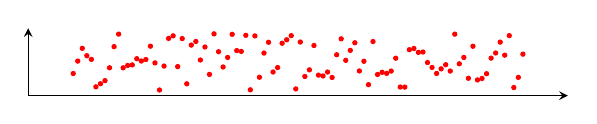
\begin{tikzpicture}[     declare function={a(\x)=0.75;},     declare function={b(\x)=0.25;} ] \begin{axis}[     domain=1:5,     axis lines=middle,     axis equal image,     xtick=\empty, ytick=\empty,     enlargelimits=true,     clip mode=individual, clip=false ] \addplot [red, only marks, mark=*, samples=100, mark size=0.75]     {0.5*(a(x)+b(x)) + 0.5*rand*(a(x)-b(x))}; \end{axis} \end{tikzpicture}

We standardize our data by first subtracting out the mean: $\mu = \frac{1}{m} \sum_{i=1}^{m} x^{(i)}$, $x -= \mu$.

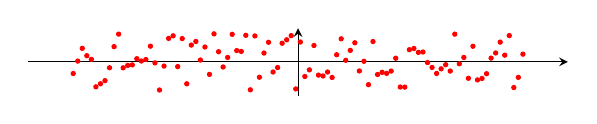
\begin{tikzpicture}[     declare function={a(\x)=0.25;},     declare function={b(\x)=-0.25;} ] \begin{axis}[     domain=-2:2,     axis lines=middle,     axis equal image,     xtick=\empty, ytick=\empty,     enlargelimits=true,     clip mode=individual, clip=false ] \addplot [red, only marks, mark=*, samples=100, mark size=0.75]     {0.5*(a(x)+b(x)) + 0.5*rand*(a(x)-b(x))}; \end{axis} \end{tikzpicture}

We then divide through by the variance, $\sigma^2 = \frac{1}{m} \sum_{i=1}^{m} x^{(i)}**2$ where we remark that the $**$ denotes element-wise multiplication and further that typically $\textrm{Var}(Z) = \mathbb E [Z^2] - \mathbb E [Z]^2$, but we've already de-meaned our random vector.
$x /= \sigma^2$.
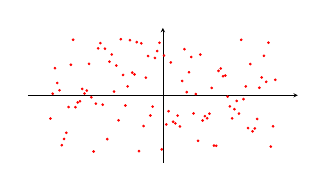
\begin{tikzpicture}[scale=0.5,     declare function={a(\x)=0.25;},     declare function={b(\x)=-0.25;} ] \begin{axis}[     domain=-.5:.5,     axis lines=middle,     axis equal image,     xtick=\empty, ytick=\empty,     enlargelimits=true,     clip mode=individual, clip=false ] \addplot [red, only marks, mark=*, samples=100, mark size=0.75]     {0.5*(a(x)+b(x)) + 0.5*rand*(a(x)-b(x))}; \end{axis} \end{tikzpicture}

We remark that the same $\mu$ and $\sigma^2$ should be used to normalize the development and test data-sets.

\paragraph{Normalization and Gradient Descent} Why should we normalize our data? It comes down to being able to apply a higher learning rate when training our algorithm. When our input data $x_1, x_2$ have very different scales (e.g. $x_1 \in [0, 1e3]$ and $x_2 \in [0,1]$), the weights learned for $w_1$ and $w_2$ will be on very different scales as well. If we plot the loss function $\mathcal L(\hat y, y)$ over $w_1, w_2$ it turns out that we end up with very elongated contours. We therefore must apply a small learning rate, leading to many small steps before convergence.

\begin{minipage}{1.0\textwidth} \begin{multicols}{2} 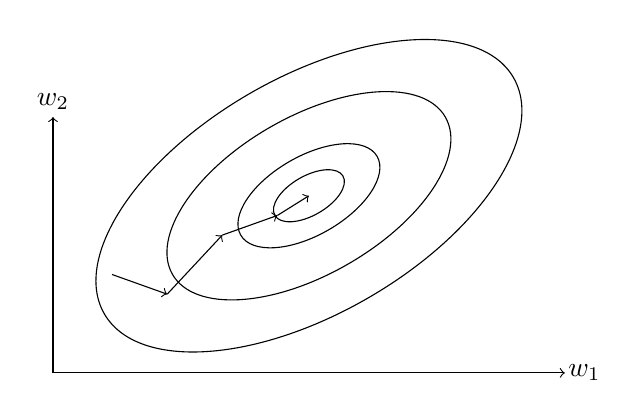
\begin{tikzpicture}
  \draw[->] (-3.25,-2.25) to (-3.25, 1);
  \node at (-3.25, 1.2) {$w_2$};
  \draw[->] (-3.25,-2.25) to (3.25, -2.25);
  \node at (3.5, -2.25) {$w_1$};
    \draw[rotate=30] (0,0) ellipse (3cm and 1.5cm); 
    \draw[rotate=30] (0,0) ellipse (2cm and 1cm);     \draw[rotate=30] (0,0) ellipse (1cm and .5cm); 
    \draw[rotate=30] (0,0) ellipse (.5cm and .25cm);
  \draw[->] (-2.5, -1) to (-1.8, -1.25);
  \draw[->] (-1.8, -1.25) to (-1.1, -.5);
  \draw[->] (-1.1, -.5) to (-.4, -.25);
  \draw[->] (-.4, -.25) to (0, 0);
\end{tikzpicture} 
\vfill\null \columnbreak
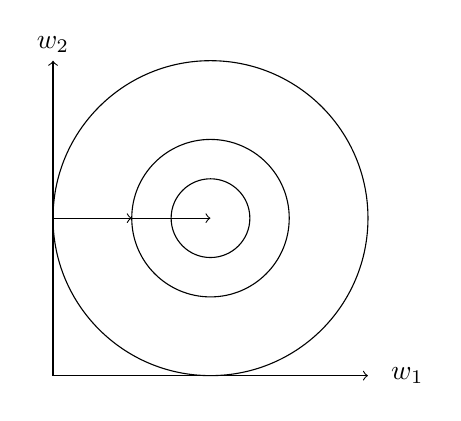
\begin{tikzpicture}[scale=2]
  \draw[->] (-1, -1) to (-1, 1);
  \node at (-1, 1.1) {$w_2$};
  \draw[->] (-1, -1) to (1, -1);
  \node at (1.25, -1) {$w_1$};
  \draw (0, 0) circle (1cm);   
  \draw (0, 0) circle (.5cm); 
  \draw (0, 0) circle (.25cm); 
  \draw[->] (-1, 0) to (-.5, 0);
  \draw[->] (-.5, 0) to (0, 0);
\end{tikzpicture}
\end{multicols} \end{minipage}

Whereas if we first normalize our inputs, the loss function when plotted over the weights appears more like a uniform bowl, and our contour plots are spherical. Our learning rate can be set higher since the step size is no longer limited by the major axis. Performing normalization never hurts our learning algorithm.

\subsection{Vanishing/Exploding gradients}
Suppose for the sake of argument that we have a very deep neural network; we've drawn only two hidden neurons per layer but this is only for illustration sake.

\begin{figure}[h]
\centering
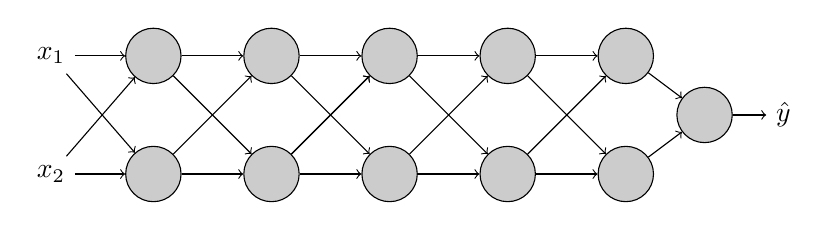
\begin{tikzpicture}[darkstyle/.style={circle,draw,fill=gray!40,minimum size=20}]
  \node (x1) at (-1.3, 1.5) {$x_1$};   \node (x2) at (-1.3, 0) {$x_2$};   
  \foreach \x in {0,...,4}     \foreach \y in {0,...,1}
      \node [darkstyle] (\x\y) at (1.5*\x,1.5*\y) {};
  \draw[->] (x1) to (00);
  \draw[->] (x1) to (01);
  \draw[->] (x2) to (00);
  \draw[->] (x2) to (01);
  \draw[->] (00) to (10);
  \draw[->] (00) to (11);
  \draw[->] (01) to (10);
  \draw[->] (01) to (11);
  \draw[->] (10) to (21);
  \draw[->] (10) to (20);
  \draw[->] (10) to (21);
  \draw[->] (11) to (20);
  \draw[->] (11) to (21);
  \draw[->] (20) to (30);
  \draw[->] (20) to (31);
  \draw[->] (21) to (30);
  \draw[->] (21) to (31);
  \draw[->] (30) to (40);
  \draw[->] (30) to (41);
  \draw[->] (31) to (40);
  \draw[->] (31) to (41);
  \node[darkstyle] (outputneuron) at (7, .75) {}; 
  \draw[->] (40) to (outputneuron);
  \draw[->] (41) to (outputneuron);
  \node (yhat) at (8, .75) {$\hat y$};
  \draw[->] (outputneuron) to (yhat);
\end{tikzpicture}
\end{figure}

Suppose we choose $g(z) = z$, i.e. a linear activation function, and suppose for sake of argument that we ignore our bias term, i.e. $b^{[\ell]} = 0$ for each layer. It's easy to see that $\hat y = W^{[L]} W^{[L-1]} \ldots W^{[2]} W^{[1]} W^{[0]} X$. Ignoring the last $W^{[L]}$ which is of different dimension, suppose each intermediary weight matrix is slightly larger than an identity matrix i.e. $\begin{bmatrix}   1 + \epsilon & 0 \\ 0 & 1 + \epsilon \end{bmatrix}$ then the value of $\hat y$ explodes with the number of layers,
$\hat y = W^{[L]} \begin{bmatrix}   (1 + \epsilon)^{L-1} & 0 \\ 0 & (1 + \epsilon)^{L-1} \end{bmatrix}X$. Similarly, if the intermediary matrices are slightly smaller than an identity matrix, then the values of subsequent activation functions get exponentially smaller. This can start to become problematic if we have $L$ quite large; in 2018 Microsoft published state of the art results using $L \approx 150$, which is large enough for these problems to manifest by slowing down gradient descent.

\subsection{Weight Initialization for Deep Networks} Suppose for the sake of illustration we have a single activation neuron.
\begin{figure}[h]
  \centering   
  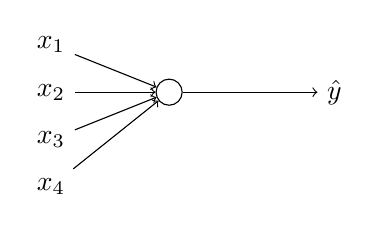
\begin{tikzpicture}[scale=0.6]
    \node (x1) at (-1, 1) {$x_1$};
    \node (x2) at (-1, 0) {$x_2$};
    \node (x3) at (-1,-1) {$x_3$};
    \node (x4) at (-1,-2) {$x_4$};
    \node[draw,circle] (neuron) at (1.5,0) {};
    \draw[->] (x1) to (neuron);
    \draw[->] (x2) to (neuron);
    \draw[->] (x3) to (neuron);
    \draw[->] (x4) to (neuron);
    \node (output) at (5,0) {$\hat y$};
    \draw[->] (neuron) to (output);
  \end{tikzpicture} 
\end{figure}
For simplicity sake, ignore $b$ for now. The input to our activation function
looks like $z = w_1 x_1 + w_2 x_2 + \ldots + w_n x_n$. So, if the number of input features (or hidden neurons in an intermediary layer) is large, we want smaller $w_i$ to compensate such that $z$ doesn't explode. One idea might be to set $\textrm{Var}(w_i) = \frac{1}{n}$ such that $\textrm{Var}(z) \approx \sum_i \textrm{Var}(x_i)$ and we preserve the variance of our input to our activation function. To accomplish this, we set
\begin{align*}   W^{[\ell]} = \texttt{np.random.randn(shape) * np.sqrt} \left(\frac{1}{n^{[\ell-1]}}\right) \end{align*}
If we're using ReLU activation functions, it's common to replace the numerator in the scaling constant above with a 2 instead of a 1 (i.e. to set $\textrm{Var}(w_i) = \frac{2}{n}$). If you want, you can consider this scaling factor to be another hyperparameter, and we can search across a sequence of values and choose the best according to our development data-set.

\subsection{Numerical Approximation of Gradients}
When performing back propagation, there is a technique known as Gradient-Checking
that will help to ensure your implementation of back propagation is correct. To 
perform gradient checking, we first need to understand how to numerically approximate
a gradient.

Suppose we have some function $f(\theta) = \theta^3$, and we choose $\epsilon = 0.01$. To compute a numerical gradient around a point $\theta$, we will use a central difference method:
\[
f'(\theta) \approx \frac{f(\theta + \epsilon) - f(\theta - \epsilon)}{2 \epsilon}.
\]
This approximation has an error that is upper-bounded by $O(\epsilon^2)$, which can be shown through a Taylor Series approximation (see \href{https://en.wikipedia.org/wiki/Finite_difference_method#Accuracy_and_order}{finite difference method}), recalling that $f'(\theta) = \lim_{\epsilon \to 0} \frac{f(\theta + \epsilon) - f(\theta - \epsilon)}{2 \epsilon}$. This is in stark contrast to taking a one-sided difference to approximate a gradient, which has error bounded by $O(\epsilon)$.

\paragraph{Gradient Checking} A technique for catching errors in a back-propagation implementation. The first step is to take
$W^{[1]}, b^{[1]}, \ldots, W^{[L]}, b^{[L]}$ and \emph{reshape} 
them into one giant vector, call it $\theta$. We may now 
equivalently define our cost function as 
 $J(W^{[1]}, b^{[1]}, \ldots, W^{[L]}, b^{[L]}) = J(\theta)$.
The next step is to take $\d W^{[1]}, \d b^{[1]}, \ldots, \d W^{[L]}, \d b^{[L]}$ (ordered the same way) and reshape them into another giant vector $\d \theta$.

\begin{algorithm}
  \caption{\texttt{Grad-check}}   \For{each $i$} {
    $\d \theta_{\texttt{approx}}^{[i]} = \frac{J(\theta_1, \theta_2, \ldots, \theta_i + \epsilon, \ldots) - J(\theta_1, \theta_2, \ldots, \theta_i - \epsilon, \ldots)}{2\epsilon}$
  } \end{algorithm}
We now end up with two vectors, each the same length, $\d \theta_{\texttt{approx}}^{[i]}$ and $\d \theta$. We can now compare them using Euclidean norms,
\begin{equation}
\label{eq: normed-diff}
\frac{\| \d \theta_{\texttt{approx}} - \d \theta\|_2}{\|\d \theta_{\texttt{approx}}\|_2 + \| \d \theta \|_2}
\end{equation}

Now, suppose we implement gradient checking with $\epsilon = 10^{-7}$. If \ref{eq: normed-diff} is $O(10^{-7})$ or smaller, then great! We've implemented back propagation correctly. If \ref{eq: normed-diff} outputs something $O(10^{-5})$, it would be prudent to check the components (elements) of $\d \theta_{\texttt{approx}} - \d \theta\|_2$ and see if any one of them is particularly large, if so we might want to double check our implementation for that layer. If, however, \ref{eq: normed-diff} outputs something $O(10^{-3})$, it's indicative of a bug in our implementation. Again, the method is to inspect the components of \ref{eq: normed-diff} to locate the source of our bug.

\paragraph{Implementation Notes for Gradient Checking}
\begin{itemize}   \item Don't use in training -- only to debug. I.e. computing $\d \theta_{\texttt{approx}}^{[i]}$ for each $i$ is expensive. Once we've verified that \ref{eq: normed-diff} outputs something sufficiently small, we should turn \emph{off} \texttt{grad-check}.
  \item If algorithm fails \texttt{grad-check}, examine individual components in order to debug. We might find that the bug is isolated to a particular layer. 
  \item Remember regularization -- if $J(\theta) = \frac{1}{m} \sum_{i=1}^m \mathcal L(\hat {y^{(i)}}, y^{(i)}) + \frac{\lambda}{2m} \sum_\ell \|W^{[\ell]}\|_F^2$ includes regularization, then we need to be sure to include this penalty term when we compute $\d \theta_{\texttt{approx}}$, since $\d \theta$ is defined as the derivative with respect to our cost function.
  \item \texttt{Grad-check} does \emph{not} work with dropout -- since dropout randomly eliminates (hidden) nodes from the network, there is no easy to compute $J(\theta)$ that dropout is doing gradient descent on.\footnote{It turns out that when using dropout, we can actually define a cost function that is defined over the exponentially large space of all possible subsets of hidden neurons, however this is computationally intractable to compute and compare with.} To get around this, we might turn \texttt{keep\_prop = 1.0} before running \texttt{grad-check}.
  \item Run at a random initialization of $W$'s and $b$'s, and perhaps again after some training -- it's possible that our (buggy) back propagation algorithm may not incur \emph{too} much error when $W, b \approx 0$, but that as our weights increase the errors do to. So, we might try running \texttt{grad-check} when we first randomly initialize $W$ and $b$, and then also again after some training has allowed our weights to drift sufficiently away from zero.  \end{itemize}

\section{Optimization Algorithms}
\subsection{Mini-batch gradient descent}
We've previously seen that matrix-multiplies allow us to efficiently compute a gradient on all $m$ training examples simultaneously. I.e., we had
\begin{equation}
  X = \begin{bmatrix}     x^{(1)} & x^{(2)} & \ldots & x^{(m)}   \end{bmatrix} \in \mathbb R^{n_x, m} \\ \hspace{15pt}
  Y = \begin{bmatrix}     y^{(1)} & y^{(2)} & \ldots & y^{(m)}   \end{bmatrix} \in \mathbb R^{1, m}.
\end{equation}

But in deep learning we often work with large data; 
what if $m$ really large, e.g. 50M? This means that we have to churn through a lot of compute before taking a very small step in gradient descent. It turns out that we can often allow our algorithm to learn faster if we allow for gradient descent to start taking palce before we're done processing all $m$ training examples.

We partition our data into mini-batches, 
each of approximately equal size. Let us use a superscript curly-brace to denote the mini-batch number. E.g. if we choose a mini-batch size of 1e3 training examples, 
our training data now looks like
\[
  X = \begin{bmatrix}       \color{purple} x^{(1)} & \color{purple} x^{(2)} & \color{purple} \ldots & \color{purple} x^{(1000)}      & \color{orange} x^{(1001)} & \color{orange} \ldots & \color{orange} x^{(2000)} & \color{black} \ldots & x^{(m)}   \end{bmatrix} \in \mathbb R^{n_x, m}
\]
and correspondingly for $Y$.
The number of mini-batches is of course given by $m/\texttt{mini-batch size}$. Mini-batch $t$ then consists of $\{X^{\{t\}}, Y^{\{t\}}\}$. The dimension of $X^{\{t\}}$ is $(n_x, \texttt{mini-batch size})$.

\begin{algorithm}[h]   \caption{Mini-batch gradient descent}
  \For{$t = 1, \ldots, m/\texttt{mini-batch size}$} {
    \tcp{One step (epoch) of gradient descent using $X^{\{t\}}, Y^{\{t\}}$.}
    $Z^{[1]} = W^{[1]} X^{\{t\}} + b^{[1]}$ \\
    $A^{[1]} = g^{[1]}(Z^{[1]})$ \\
    $\vdots$ \\
    $A^{[L]} = g^{[L]}(Z^{[L]})$
    $J^{\{t\}} \gets \frac{1}{\texttt{mini-batch size}} \sum_{i=1}^{\texttt{mini-batch size}} \mathcal L(\hat y^{(i)}, y^{(i)}) + \frac{\lambda}{2 \cdot \texttt{mini-batch size}} \sum_{\ell = 1}^{L} \|W^{[\ell]}\|_F^2$ \\
    \tcp{Backpropagation to compute gradients w.r.t. $J^{\{t\}}$ (using $X^{\{t\}}, Y^{\{t\}}$).}
    $W^{[\ell]} := W^{[\ell]} - \alpha \d W^{[\ell]}$
    $b^{[\ell]} := b^{[\ell]} - \alpha \d b^{[\ell]}$
  } \end{algorithm}

With larger data sets, mini-batch gradient descent is likely to converge much faster.

\subsubsection{Understanding mini-batch gradient descent}
With (vanilla) batch gradient descent, we expect that the loss
function should be monotone decreasing with respect to the 
number of iterations of gradient descent. E.g.
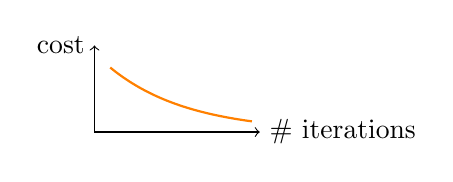
\begin{tikzpicture}
\draw[->] (0, 0) to (0, 1.1) node [left] {cost}; \draw[->] (0, 0) to (2.1, 0) node [right]{\# iterations}; 
\draw[smooth, domain=0.2:2, color=orange, thick]      plot (\x,{exp(-\x)}) {};
\end{tikzpicture}
When we train on a cost function $J^{\{t\}}$, it depends on
$X^{\{t\}}, Y^{\{t\}}$ which vary with each iteration. And so
it's not the case that we expect our cost function to 
monotonically decrease with each iteration of mini-batch gradient descent. We should see something that is (hopefully) sinusoidal and downward trending, e.g.
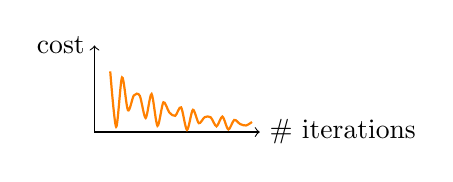
\begin{tikzpicture}
\draw[->] (0, 0) to (0, 1.1) node [left] {cost}; \draw[->] (0, 0) to (2.1, 0) node [right]{\# iterations};
\draw[smooth, domain=0.2:2, color=orange, thick]
plot (\x,{exp(-\x)*abs(cos(\x*1000))}) {};
\end{tikzpicture}. Why does our learning plot have this shape? It could be the case that the first epoch of data $X^{\{1\}}, Y^{\{1\}}$ was ``easier'' to predict on relative to a latter epoch.


\subsubsection{Choosing mini-batch size}
One point worth discussing is how to choose your mini-batch size. If we select $\texttt{mini-batch size} = m$, then we recover gradient descent. On the other extreme, we can set the \texttt{mini-batch size} to $1$, in which case we get 
\href{https://en.wikipedia.org/wiki/Stochastic_gradient_descent}{Stochastic Gradient Descent}, in which case each 
training example is its own mini-batch. Let's consider these two extremes as applied to the following hypothetical loss function (and corresponding contours).
{
\begin{figure}[h]
\centering
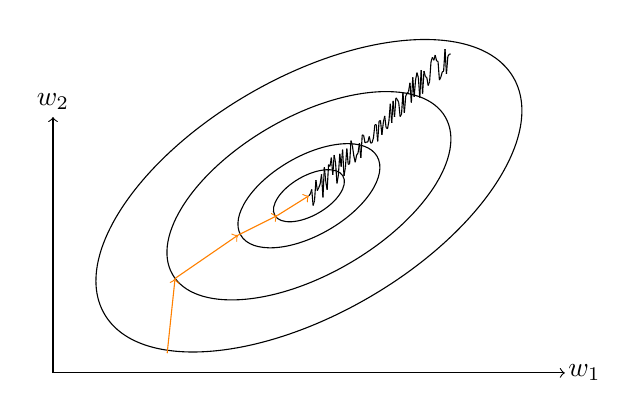
\begin{tikzpicture}
      \draw[->] (-3.25,-2.25) to (-3.25, 1);
      \node at (-3.25, 1.2) {$w_2$};
      \draw[->] (-3.25,-2.25) to (3.25, -2.25);
      \node at (3.5, -2.25) {$w_1$};
      \draw[rotate=30] (0,0) ellipse (3cm and 1.5cm); 
      \draw[rotate=30] (0,0) ellipse (2cm and 1cm);     \draw[rotate=30] (0,0) ellipse (1cm and .5cm); 
      \draw[rotate=30] (0,0) ellipse (.5cm and .25cm);
  \draw[->,orange] (-1.8, -2) to (-1.7, -1.05);
  \draw[->,orange] (-1.7, -1.05) to (-.9, -.5);
  \draw[->,orange] (-.9, -.5) to (-.4, -.25);
  \draw[->,orange] (-.4, -.25) to (0, 0);
  \NewDocumentCommand{\irregularline}{O {2mm} m m D <> {20}}{{       \coordinate (old) at #2;       \foreach \i in {1,2,...,#4}{         \draw (old) -- ($ ($#2!\i/(#4+1)!#3$) + (0,#1*rand) $) coordinate (old);       }       \draw (old) -- #3;     }}
  \irregularline{(0,0)}{(1.8,1.8)}<100>
\end{tikzpicture} 
\end{figure}
}

We've drawn vanilla gradient descent (in \color{orange}{orange}\color{black}) taking a few easy steps through the training data, each time moving toward the 
(global) minimum. On the other hand stochastic gradient descent (which we've drawn starting from a different initialization point for the sake of illustration) 
doesn't always get the direction right and in fact the path may be
far more circuitous than what we've shown. In fact, SGD won't even ever hit the global minimum (or ``converge''), it is far more likely to simply ``dance around'' the global minimum within some reasonably tight radius.

\paragraph{Advantages of mini-batch gradient descent}
In reality, we choose a mini-batch size in between 1 and $m$. If we were to choose $m$, the time required for each step of 
training would be too large (assuming large data). If we were to choose SGD, the downside is that we lose almost all speed-up from 
vectorization, since we process only one example at a time. With mini-batch gradient descent, we do get some 
vectorization (speed-up relative to processing one example at a time), and secondly we can make progress without 
waiting to process the entire training set. Further, with mini-batch gradient descent we won't take as circuitous a 
route before approaching the global optimum (which again we will not hit exactly).

\begin{itemize}   
  \item If training set is small (e.g. less 2,000 observations), just use batch gradient descent since the whole training set can be processed quite quickly.
  \item Otherwise, consider picking a mini-batch size equal to a power of two, such that hopefully data can 
    be loaded and stored in cache (or GPU memory), perhaps in the set $\{2^6, \ldots, 2^9\}$. 
\end{itemize}

\subsection{Momentum and Exponentially Weighted (moving) Averages} There are faster algorithms relative to mini-batch gradient descent.
To understand them, we need to understand \href{https://en.wikipedia.org/wiki/Moving_average#Exponential_moving_average}{exponentially weighted averages}. Suppose we have a time-series dataset  $x_1, \ldots, x_T$; we might estimate a moving average as follows:
\begin{align}
  \label{eq: expmovavg}   v_0 &= 0 \nonumber \\
  v_i &= 0.9 * v_{i-1} + 0.1 * x_i \hspace{35pt} \texttt{for } i > 0. \end{align}

We can make this a little bit more interesting by choosing some $\beta$ and then setting our update rule to become $v_i = \beta * v_{i-1} + (1-\beta) * x_i$. It can be shown that $v_t$ is an average over approximately $\frac{1}{1-\beta}$ points of data. As we set $\beta \approx 1$, we average over more points of data and get a \emph{smoother} time-series. The downside of averaging over more points is that we learn the trend of our data \emph{slower} (and therein incur a higher latency bias).

\paragraph{Math behind exponentially weighted averages} Let's unroll our formula to 
gain an intuition for what's happening. Suppose we have 100 data points.
\begin{align*}   v_{100} &= \beta v_{99} + (1-\beta) x_{100} \\
  v_{99}  &= \color{purple} \beta v_{98} + (1-\beta) x_{99} \\ 
  &\ldots \end{align*}
Then we can rewrite our last value as 
\[
  v_{100} = (1-\beta) x_{100} + \beta \left( \color{purple} (1-\beta) x_{99} + \beta v_{98} \color{black} \right) 
\]
and continuing to unroll term-by-term we see that
\[
  v_{100} = (1-\beta) x_{100} + (1-\beta) \beta x_{99} + (1-\beta) \beta^2 x_{98} + (1-\beta) \beta^3 x_{97} + \ldots.
\]

Put differently, the time series of data-points $v_i$ are generated by taking the element-wise product of our original time series with an exponentially decaying function which places the most weight on the most recent data point (and decaying weight to older data points). The coefficients add up to one, less a bias term that will be discussed later. In practice, to compute \ref{eq: expmovavg}- we only need to store a single real number in memory which we continuously update to take on the latest value of 
the moving average (based on its last value and the most recent data).

\paragraph{Bias correction in exponentially weighted (moving) averages} Let's consider our recurrence \ref{eq: expmovavg}. Notice that since we initialize $v_0 = 0$, and since $\beta \in (0,1)$, then
\begin{align*}   v_1 = \underbrace{\beta v_0}_{=0} + (1-\beta) x_1 \implies v_1 < x_1
%  v_2 = \beta v_1 + (1-\beta) x_2 = \beta (1-\beta) x_1 + (1-\beta) x_2 = (1-\beta) \left(\beta x_1 + x_2\right)
\end{align*}
we see that we incur a bias in our first point estimate. This persists until our moving average ``learns'' enough from the past data. To make our estimate more accurate during the initial phase, we take $v_t$ and scale it as follows:
\[
  \frac{v_t}{1 - \beta^t}.
\]
When $t$ is large, this bias correction fades away, but when $t$ is small it can really help.

\paragraph{Gradient descent with momentum} The idea is to compute an exponentially weighted average of gradients, and to use this to update our weights; it's almost always faster when compared with vanilla gradient descent. As an example, let's consider the following cost function with corresponding contours; starting from an arbitrary point, we might expect (mini) batch gradient descent to behave in the following way.

\begin{figure}[h]
\centering
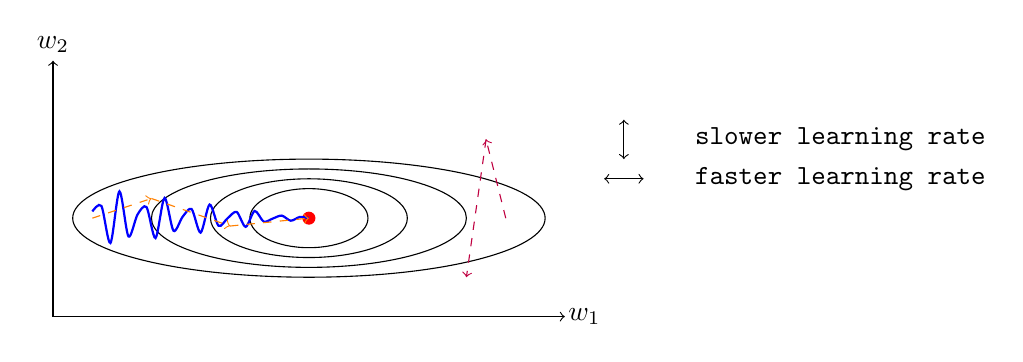
\begin{tikzpicture}
  \draw[->] (-3.25,-2.25) to (-3.25, 1);
  \node at (-3.25, 1.2) {$w_2$};
  \draw[->] (-3.25,-2.25) to (3.25, -2.25);
  \node at (3.5, -2.25) {$w_1$};
  \draw (0,-1) ellipse (3cm and .75cm); 
  \draw (0,-1) ellipse (2cm and .625cm);     
  \draw (0,-1) ellipse (1.25cm and .5cm); 
  \draw (0,-1) ellipse (.75cm and .375cm);
  \node[fill,red,circle,scale=0.5] at (0,-1) {};
  \draw[smooth, domain=-2.75:-.00125, color=blue, thick]
    plot (\x,{1/7*abs(\x)*sin((\x-3)*1250)-1}) {};
  \draw[->,purple,dashed] (2.5,-1) to (2.25, 0);
  \draw[->,purple,dashed] (2.25,0) to (2, -1.75);
  \draw[<->] (4, .25) to (4, -.25);
  \node at (6.75, 0) {\texttt{slower learning rate}};
  \draw[<->] (3.75, -.5) to (4.25, -.5);
  \node at (6.75, -.5) {\texttt{faster learning rate}};
  \draw[->,orange,dashed] (-2.75,-1) to (-2, -.75);
  \draw[->,orange,dashed] (-2, -.75) to (-1, -1.1);
  \draw[->,orange,dashed] (-1, -1.1) to (0, -1);
\end{tikzpicture}
\end{figure}

Notice that initially in this gradient descent trajectory, 
we tend to end up ``on the other side of the 
ellipse'' than intended, this process repeats and 
we end up \emph{oscillating} toward the minimum.
If we try to use a \emph{larger} learning rate, we are likely
to \emph{diverge} (pictured in \color{purple}{purple} 
above\color{black}).
This forces us to use a learning rate that is not too large.
Another way to view this problem, is that on the vertical 
axis, we'd like slower learning, but on the horizontal axis 
we'd like faster learning. This is because the shape of the contours make it easier to ``overshoot'' and end up with a larger cost value when moving up and down relative to left and right.

\paragraph{Momentum} On iteration $t$, we compute $\d W$, $\d b$ on current (mini)-batch. Then, compute
\begin{align*}
V_{\d W} &= \beta V_{\d W} + (1-\beta) \d W \\
V_{\d b} &= \beta V_{\d b} + (1-\beta) \d b
\end{align*}
Our update rule then becomes
\begin{align*}
W &:= W - \alpha V_{\d W} \\
b &:= b - \alpha V_{\d b}
\end{align*}
This has the effect of ``smoothing out'' our steps of gradient descent and in particular it dampens the oscillations that we previously saw. Why is this? Well, if we previously had many up and down oscillations, the average gradient is near zero, whereas on the other hand we are always moving consistently toward the global minimum from left to right and so the weighted average still pulls strongly in this direction; we've plotted this in \color{orange}{orange} \color{black} above.

\paragraph{Intuition} Suppose we have a bowl shaped loss function, and that we plan to roll a ball ``downhill'' toward the global minimum. The terms $\d W$ and $\d b$ describe \emph{acceleration} that we place on the ball, whereas the terms $\beta V_{\d W}$ and $\beta V_{\d b}$ describe \emph{velocity} and in particular wince 
$\beta < 1$ we have a notion of \emph{friction} which prevents
our ball from rolling too fast or out of control.

\paragraph{Hyperparameters} Notice that we've added an additional hyperparameter $\beta$ which controls the exponentially weighted average. The most common value Andrew Ng reports for $\beta$ is 
0.9, which corresponds to averaging over the last $1/(1-.9) = 10$ 
gradients.

\subsection{RMSProp} Momentum was one method of speeding up gradient descent. There's another known as Root Mean Square Prop. On iteration $t$ of (mini) batch gradient descent, we compute the following (where here $\cdot^2$ denotes an element-wise squaring operation.
\begin{align*}   S_{\d W} &= \beta S_{\d W} + (1-\beta) \d W^2 \\ %\hspace{15pt} \tcp{Element-wise square}
  S_{\d b} &= \beta S_{\d b} + (1-\beta) \d b^2 \\ %\hspace{15pt} \tcp{Again, element-wise square}
  W &:= W - \alpha \frac{\d W}{\sqrt{S_{\d W}} + \epsilon} \\
  b &:= b - \alpha \frac{\d b}{\sqrt{S_{\d b}} + \epsilon} \end{align*}

Adam stands for Adaptive Moment Estimation. $\beta_1$ is used to compute the mean of the gradients $\d W$ (first moment) and $\beta_2$ is used to compute the mean of the second moments $\d W^2$.

\paragraph{Intuition}
Notice that it's in the update step where a RMS term appears.
Why does this work? Recall our previous example where in the vertical direction we wanted a smaller learning rate, but for the horizontal direction we wanted a larger learning rate. By incorporating the square of the gradient, we can achieve similar outcomes as with momentum (\emph{dampening gradients that oscillate wildly}).

\paragraph{Implementation Details} In practice, we add some $\epsilon \approx 1e-8$ to the denominator such that we don't divide by something too close to zero (causing our update to blow up).

\subsection{Adam} This is a rare instance of an algorithm that actually works; it works by combining momentum with RMSProp. We first initialize parameters:
\begin{align*}   V_{\d W} = 0, S_{\d W} = 0, V_{\d b} = 0, S_{\d b} = 0 \end{align*}
Then, on iteration $t$, we compute 
$\d W$, $\d b$ using current mini-batch, and then
\begin{align*}   V_{\d W} &= \beta_1 V_{\d W} + (1-\beta_1) \d W \\ 
  V_{\d b} &= \beta_1 V_{\d b} + (1-\beta_1) \d b \\ 
  S_{\d W} &= \beta_2 S_{\d W} + (1-\beta_2) \d W^2 \\
  S_{\d b} &= \beta_2 S_{\d b} + (1-\beta_2) \d b^2 \end{align*}
Typically, we do implement Adam by using $V^{\texttt{corrected}}_{\d W} = \frac{V_{\d W}}{1-\beta_1^t}$ and $V^{\texttt{corrected}}_{\d b} = \frac{V_{\d b}}{1 - \beta_1^t}$ and similarly we have
$S^{\texttt{corrected}}_{\d W} = \frac{S_{\d W}}{1-\beta_2^t}$ and $S^{\texttt{corrected}}_{\d b} = \frac{S_{\d b}}{1-\beta_2^t}$. Then, we perform the updates
\begin{align*}   W &:= W - \alpha \frac{V^{\texttt{corrected}}_{\d W}}{\sqrt{S^{\texttt{corrected}}_{\d W}} + \epsilon} \\
  b &:= b - \alpha \frac{V^{\texttt{corrected}}_{\d b}}{\sqrt{S^{\texttt{corrected}}_{\d b}} + \epsilon} \end{align*}
\paragraph{Hyperparameters}
There are now multiple hyperparameters.
\begin{itemize}   \item $\alpha$ is a hyperparameter that typically needs to be tuned.
\item $\beta_1 \gets 0.9$, i.e. for $\d W$ we average over last ten gradients.
\item $\beta_2 \gets 0.999$, i.e. for $\d W^2$ we average over the last $\frac{1}{1 - 0.999} = 1,000$ gradients.
\item $\epsilon \gets 1e-8$ is typically fixed. \end{itemize}

\subsection{Learning Rate Decay} The idea here is that we take larger steps at first (making steady progress toward the global minimum), but as we approach we start taking smaller steps so as to avoid the problem of dancing around in circles a far region away from the global minimum. To implement learning rate decay, we may choose a heuristic where $\alpha = \frac{1}{1 + \texttt{decay\_rate}*\texttt{epoch\_\#}} \alpha_0$. As a function of the epoch number, this formula (dependent on hyperparameter $\alpha_0$) decays steadily. Another few formulae people try are
\begin{align*}   \alpha &= 0.95^{\texttt{epoch\#}} \cdot \alpha_0 \\
  \alpha &= \frac{k}{\sqrt{\texttt{epoch\#}}} \cdot \alpha_0 \\
  \alpha &= \frac{k}{\sqrt{t}} \cdot \alpha_0 \end{align*}

\subsection{Local Optima} As the field of deep learning has evolved, so has the way we think about local optima. People used to examine low (three) dimensional plots in which it's easy to create many local optima that are significantly worse than the global optimum. In reality in deep learning our parameters $b, W$ live in very high dimensions; in these cases, we are much more likely to run into saddle points as opposed to local optimum. What is a problem in higher dimensions are \emph{plateaus}, and this slows down learning. It is in these cases of plateaus that faster learning algorithms like Adam can really help out.

\subsection{Hyperparameter tuning} Changing a neural network can involve modifying many hyperparameters.
This section is on how to systematically organize your hyperparameter tuning process. The sheer number of hyperparameters
can feel overwhelming: learning rate $\alpha$, momentum term $\beta$, or even additional parameters $\beta_1, \beta_2$ and $\epsilon$ 
if using Adam. Perhaps we additionally need to pick the number of layers, the number of hidden units, whether to use a learning
rate decay, and additionally a mini-batch size.

\paragraph{Random Search}
It turns out that of the many hyperparameters, only a few consequentially matter. Perhaps $\alpha$, 
the learning rate $\alpha$, is the 
\emph{most} important. Momentum terms and mini-batch size are also often times worthwhile to consider next, 
followed by the number of 
hidden units. Lastly, a standard recommendation may be to finally 
consider the number of layers and whether to use learning rate decay. 
Whereas it used to 
be common practice to conduct a \emph{grid-search}, it is now recommended to 
search over the same space
\emph{at random}. If we were going to sample $k$ points on a lattice before, we can still sample the same 
number of points at 
random, however by sampling at random we allow ourselves to try more \emph{unique} values of 
each hyperparameter, which is 
crucial since we don't know in advance which are important for a given task. For more details see
\href{http://www.jmlr.org/papers/volume13/bergstra12a/bergstra12a.pdf}{Bergstra and Bengio '12}.

\begin{minipage}{1.0\textwidth} 
  \begin{multicols}{2} 
    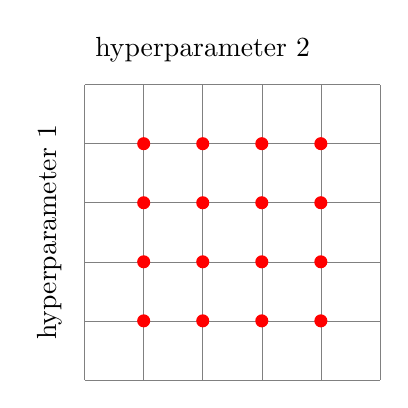
\begin{tikzpicture}[scale=0.75]
      \draw[step=1cm,gray, very thin] (0, 0) grid (5, 5);
      \node[rotate=90] at (-0.6, 2.5) {hyperparameter 1};
      \node            at (2,5.6) {hyperparameter 2};
      \foreach \x in {1, ..., 4} {
        \foreach \y in {1, ..., 4} {
          \node[circle, fill, red, scale=1/2] at (\x, \y) {};
        }
      }
    \end{tikzpicture} 
\vfill\null \columnbreak
\begin{tikzpicture}[     
  declare function={a(\x)=1.7;},     
  declare function={b(\x)=0.1;} ] 
  \begin{axis}[     
    domain=0:2,     
    axis lines=middle,     
    axis equal image,     
    xtick=\empty, 
    ytick=\empty,     
    enlargelimits=true,     
    clip mode=individual, 
    clip=false 
    ] 
    \addplot [red, only marks, mark=*, samples=16, mark size=1]     {0.5*(a(x)+b(x)) + 0.5*rand*(a(x)-b(x))}; 
  \end{axis} 
  \node[rotate=90] at (-0.2, 2.5) {hyperparameter 1};
  \node            at (3.5,-.4)   {hyperparameter 2};
\end{tikzpicture}
\end{multicols} 
\end{minipage}

In practice, we search over more than two (hyperparameters) dimensions; if we search over a grid we suffer from
 the curse of dimensionality.

\paragraph{Coarse-to-fine sampling schemes} Andrew also recommends using a coarse-to-fine sampling schema.
To do this, first apply random sampling to a larger region, and then once a sub-region has been identified
which corresponds to low values of the cost function we can focus more compute resources on a smaller \color{blue}{area}\color{black}.

\begin{figure}[h]
\centering
\begin{tikzpicture}[     
  declare function={a(\x)=1.7;},     
  declare function={b(\x)=0.1;},
  declare function={c(\x)=0.4;},
  declare function={d(\x)=0.7;}
] 
\pgfmathsetseed{4}
  \begin{axis}[     
    domain=0:2,     
    axis lines=middle,     
    axis equal image,     
    xtick=\empty, 
    ytick=\empty,     
    enlargelimits=true,     
    clip mode=individual, 
    clip=false 
    ] 
    \addplot [red, only marks, mark=*, samples=16, mark size=1]     {0.5*(a(x)+b(x)) + 0.5*rand*(a(x)-b(x))}; 
    \addplot [domain=1:1.5, blue, only marks, mark=+, samples=25, mark size=1]     {0.5*(c(x)+d(x)) + 0.5*rand*(c(x)-d(x))}; 
  \end{axis} 
  \node[rotate=90] at (-0.2, 2.5) {hyperparameter 1};
  \node            at (3.5,-.4)   {hyperparameter 2};
  \draw[blue,dashed] (3.25, .75) -- (5,.75) -- (5, 1.75) -- (3.25, 1.75) -- (3.25, .75);
\end{tikzpicture}
\end{figure}

\subsection{Using an appropriate scale to pick hyperparameters} Sampling at random doesn't in fact mean
sampling \emph{uniformly} at random over the range of possible values, 
but instead it's important to carefully select the \emph{scale} over which we search. If it's the case that our search space (in a single dimension) is small, it is acceptable to sample uniformly at random or even perform a grid search: e.g. if we know that the number of layers $L$ should be in the set $\{2, 3, 4\}$, or if we believe the right number of hidden neurons to be between 50 and 100. However, consider a learning rate parameter $\alpha$: we may believe its optimal value to lie somewhere in the interval $(0.001, 1)$. If we sample uniformly at random, we spend 90\% of our resources searching the interval $[0.1, 1)$ and only 10\% searching the smaller end of the interval. This could be problematic. Instead, we may search for (a learning rate) parameters on a \emph{log} scale which in our example might look like $\{0.0001, 0.001, 0.01, 0.1, 1\}$.

\paragraph{Sampling on a log-scale}
How do we implement sampling on a log-scale? It's simple, take the two endpoints of the interval 
we wish to sample from and take the logarithm of each term. The resulting pair of real numbers gives another interval
which we can sample over uniformly at random. Then, after sampling we can exponentiate to get back to our original scale. E.g. $\log_{10}(0.0001) = -4$ and $\log_{10}(1) = 0$. So, we sample from $[-4, 0]$ uniformly at random, and then take these values and apply the transform $f(x) = 10^x$ to recover our desired scale.

\paragraph{Momentum and log scale sampling} Suppose we believe the best value of $\beta$ to lie in the interval
$(0.9, 0.999)$. Realize that this corresponds to averaging over the last 10 or 1,000 values. Therefore, it doesn't make sense to sample uniformly at random from this interval.

\paragraph{Tips and tricks for organizing hyperparameter searches} Intuitions do get stale, so we must 
re-evaluate them occasionally. There are two main methods for improving our models. The first is to ``babysit''
a single model, e.g. we watch the loss function day by day and with each passing day we make a subtle change to our
modeling architecture. On the other hand, we could train many models in parallel and overlay their loss functions
in different colors, choosing the best accordingly. If you have enough compute to train models in parallel, take the ``Caviar'' approach whereby we train many models and choose the best according to a development set. If we don't have a lot of compute, we can babysit the model like a Panda with their offspring.

\subsection{Batch Normalization}
Batch normalization is an algorithm created by Sergey Ioffe and Christian Szegedy, which is designed to make the
hyperparameter search problem a bit simpler whilst also making your network more robust to a \emph{wider range} 
of hyperparameter values. Recall that when training
a model like Logistic regression, we first normalized our input features such that a loss function 
with elongated contours is transformed to one more round and bowl-like which is easier for gradient descent to
optimize over.

\begin{minipage}{1.0\textwidth} 
\begin{multicols}{3}
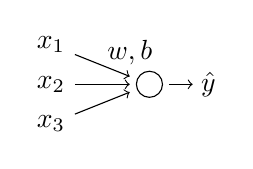
\begin{tikzpicture}
  \node (x1) at (0, 1) {$x_1$};
  \node (x2) at (0,.5) {$x_2$};
  \node (x3) at (0, 0) {$x_3$};
  \draw[->] (x1) to (1, .6);
  \draw[->] (x2) to (1, .5);
  \draw[->] (x3) to (1, .4);
  \node[draw=black,circle] (z) at (1.25, .5) {};
  \node (params) at (1, .9) {$w,b$};
  \draw[->] (1.5,.5) to (1.8, .5);
  \node at (2, .5) {$\hat y$};
\end{tikzpicture}
\columnbreak
\begin{align*}   \mu &\gets \frac{1}{m} \sum_{i=1}^m x^{(i)} \\
  x &\gets x - \mu \\
  \sigma^2 &\gets \frac{1}{m} \sum_{i=1}^m (x^{(i)})^2 \hspace{10pt} {\footnotesize \texttt{element-wise squaring}} \\
  x &\gets \frac{x}{\sigma^2} \end{align*}
\vfill\null \columnbreak
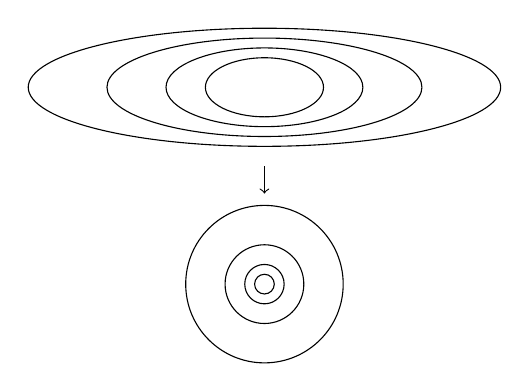
\begin{tikzpicture}
  \draw (0,1) ellipse (3cm and .75cm); 
  \draw (0,1) ellipse (2cm and .625cm);     
  \draw (0,1) ellipse (1.25cm and .5cm); 
  \draw (0,1) ellipse (.75cm and .375cm);
  \draw[->] (0,0) to (0, -.35);
  \draw (0,-1.5) circle (1cm);
  \draw (0,-1.5) circle (.5cm);
  \draw (0,-1.5) circle (.25cm);
  \draw (0,-1.5) circle (.125cm);
\end{tikzpicture}
\end{multicols} 
\end{minipage}

Batch normalization is the idea of \emph{normalizing} outputs from hidden layers; there is some debate
in the deep learning community about whether to apply the normalization before or after the activation function (i.e.
do we apply to $z_i$ or $a_i$), but normalizing $z_i$'s is done more often. The core question at heart is: can we normalize $a^{[i]}$ (or $z^{[i]}$) in such a way that we train $W^{[i]}$ and $b^{[i]}$ faster.

\subsubsection{Normalizing activations in a network} 
To implement batch normalization, suppose that we are given some
hidden unit values $z^{(1)}, \ldots, z^{(m)}$, where we have omitted the superscript square bracket $[\ell]$ indicating
which layer we are concerned with since this example just focuses on an arbitrary layer; if we wanted to be rigorous we could write this out with full notation as $z^{[\ell](1)}, \ldots, z^{[\ell](m)}$. In any case, we compute a mean and variance for the inputs to the activation function for the layer and we normalize:
\begin{align*}   \mu = \frac{1}{m} \sum_{i=1}^{m} z^{(i)}, \hspace{15pt}
  \sigma^2 = \frac{1}{m} \sum_{i=1}^m \left(z_i - \mu\right)^2, \hspace{15pt}
  z^{(i)}_{\texttt{norm}} = \frac{z^{(i)} - \mu}{\sqrt{\sigma^2 + \epsilon}} \end{align*}
where we have taken care to inflate our denominator by some fixed $\epsilon$ in the event that an estimate for
$\sigma^2$ turns out identically zero. After this transformation, each component of our vector $z$ will have 
zero mean and unit variance. However, we don't \emph{always} want the hidden units to follow a distribution
with these first two moments; instead, we compute
\[
\tilde{z^{(i)}} = \gamma z^{(i)}_{\texttt{norm}} + \beta
\]
where $\gamma$ and $\beta$ are learnable parameters of the model. I.e. for whatever optimization algorithm 
we employ, whether it be gradient descent or RMSprop or Adam, we update $\gamma$ and $\beta$ in the same way that
we update $W$'s and $b$'s. Notice that we could theoretically recover our original input to $a^{[\ell]}$ if we set 
$\gamma$ to $\sqrt{\sigma^2+\epsilon}$ and $\beta$ to $\mu$. However, we're also free to learn
parameters $\gamma$ and $\beta$ such that $\tilde{z^{(i)}}$ has an arbitrary mean and variance. 

\paragraph{Why might we prefer
the first two moments of $\tilde{z^{(i)}}$ to be different from zero and one?} Well, suppose we're using 
a sigmoid activation function. Then, in order to take advantage of the non-linearities of the function we'd
like \emph{not} to squish our input values to a range concentrated around the origin since this is where the 
activation function behaves linearly.

\begin{figure}[h]
\centering
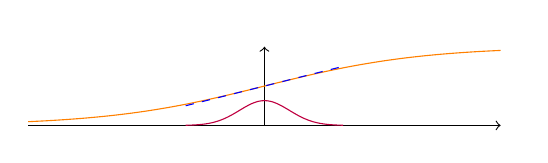
\begin{tikzpicture}
  \draw[->] (-3,0) -- (3,0) node[right] {};   
  \draw[->] (0, 0) -- (0,1) node[above] {};
  \draw[domain=-3:3,smooth,variable=\x,orange] plot ({\x},{1 / (1 + (exp(-\x)))}); 
  \draw[domain=-1:1,smooth,variable=\x,purple] plot ({\x},{1/4*1 / sqrt(2*pi*1/10) * exp(-(\x)^2/(2*1/10))}); 
  \draw[domain=-1:1,smooth,variable=\x,blue,dashed] plot ({\x},{1/4 * \x + 1/2}); 
\end{tikzpicture}
\end{figure}
Instead, perhaps we might like to enforce a larger variance such that we can explore areas of the activation function which are non-linear. In any case, the learning algorithm is free to set $\gamma$ and $\beta$ in such a way that 
it converges more quickly.

\subsubsection{Fitting batch-norm into a neural network} 
Recall that each neuron in a network computes two quantities:
a linear combination using $W, b$ to yield $z$ which is then used as input to an activation function.

\begin{figure}[h]
\centering
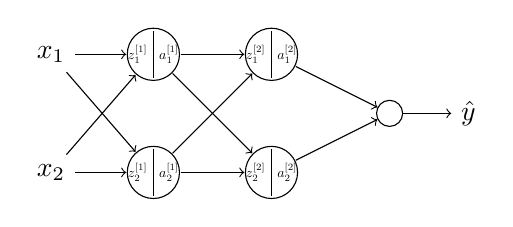
\begin{tikzpicture}[darkstyle/.style={circle,draw,fill=gray!40,minimum size=20}]
  \node (x1) at (-1.3, 1.5) {$x_1$};   \node (x2) at (-1.3, 0) {$x_2$};   
  \foreach \x in {0, 1} {
    \foreach \y in {0,...,1} {
      \node[draw,circle,scale=2]  (\x\y) at (1.5*\x,1.5*\y) {};
      \draw (1.5*\x,1.5*\y-.3) -- (1.5*\x,1.5*\y+.3);
    }
  }
  \node[scale=0.5] at (-.2, 1.5) {$z^{[1]}_1$};
  \node[scale=0.5] at (0.2, 1.5) {$a^{[1]}_1$};
  \node[scale=0.5] at (-.2, 0) {$z^{[1]}_2$};
  \node[scale=0.5] at (0.2, 0) {$a^{[1]}_2$};
  \node[scale=0.5] at (1.5-.2, 1.5) {$z^{[2]}_1$};
  \node[scale=0.5] at (1.5+0.2, 1.5) {$a^{[2]}_1$};
  \node[scale=0.5] at (1.5-.2, 0) {$z^{[2]}_2$};
  \node[scale=0.5] at (1.5+0.2, 0) {$a^{[2]}_2$};
  \draw[->] (x1) to (00);
  \draw[->] (x1) to (01);
  \draw[->] (x2) to (00);
  \draw[->] (x2) to (01);
  \draw[->] (00) to (10);
  \draw[->] (00) to (11);
  \draw[->] (01) to (10);
  \draw[->] (01) to (11);
  \node[draw,circle] (outputneuron) at (3, .75) {}; 
  \draw[->] (10) to (outputneuron);
  \draw[->] (11) to (outputneuron);
  \node (yhat) at (4, .75) {$\hat y$};
  \draw[->] (outputneuron) to (yhat);
\end{tikzpicture}
\end{figure}

Our computation graph for our input now through the first layer now looks like:

\begin{figure}[h]
\centering
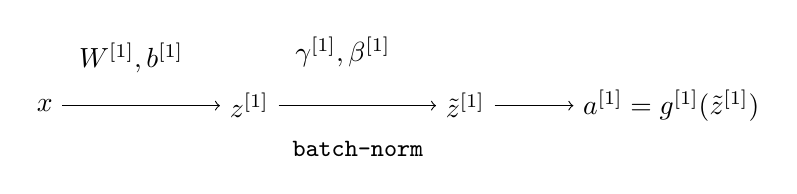
\begin{tikzpicture}   \node (x) at (0,0) {$x$};
  \node[right = 2cm of x] (z1) {$z^{[1]}$};
  \node[right = 2cm of z1] (zt) {$\tilde z^{[1]}$};
  \node[right = 1cm of zt] (a1) {$a^{[1]} = g^{[1]}(\tilde z^{[1]})$};
  \node[above right = 0.125cm of x] (w) {$W^{[1]}, b^{[1]}$};
  \node[above right = 0.125cm of z1] (beta) {$\gamma^{[1]}, \beta^{[1]}$};
  \node[below right = 0.075cm of z1] (bn)   {{\small\texttt{batch-norm}}};
  \draw[->] (x) to (z1);
  \draw[->] (z1) to (zt);
  \draw[->] (zt) to (a1);
\end{tikzpicture}
\end{figure}
We then feed-forward the outputs of $a^{[1]}$ into the inputs of $z^{[2]}$, which is governed by 
learnable parameters $W^{[2]}, b^{[2]}$, after which we perform another batch-norm governed by learnable
parameters $\gamma^{[2]}$ and $\beta^{[2]}$. This normalized $\tilde z^{[2]}$ is used to compute $a^{[2]}$, and we 
continue in this fashion through the remainder of the network if desired.

\paragraph{Parameters for a batch-norm network}
Note that the parameters of our network used to only contain $W^{[1]}, b^{[1]}, \ldots, W^{[L]}, b^{[L]}$ but now 
additionally contain $\gamma^{[1]}, \beta^{[1]}, \ldots, \gamma^{[L]}, \beta^{[L]}$. To be clear, these $\beta$'s are 
completely different from the terms used in momentum, Adam, and RMSProp.

\paragraph{Working with mini-batches} So far, we've pretended that we are using vanilla gradient descent, 
processing our entire dataset each iteration. In practice, batch-norm is often used alongside mini-batch gradient
descent, for example. In this case, on our first iteration of mini-batch gradient descent we use
$X^{\{1\}}$ as input and feed-forward through our network (applying batch-norm at each layer if desired). Then, on the
second iteration of mini-batch gradient descent we use $X^{\{2\}}$ as input, where now the batch-norm computations depend only on this input (and its intermediary transforms) but no longer on $X^{\{1\}}$. I.e. batch-norm at each iteration of mini-batch gradient descent should only depend on the current mini-batch of data and none others.

\paragraph{Parameters of a network which utilizes batch-norm} We've so far acted as though our parameters for a
layer $\ell$ are $W^{[\ell]}$, $b^{[\ell]}$, $\gamma^{[\ell]}$, and $\beta^{[\ell]}$. However, realize that 
$z^{[\ell]} = W^{[\ell]} a^{[\ell-1]} + b^{[\ell]}$, and that the subsequent step in batch-norm is to subtract out a mean and then later perform a translation via $\beta^{[\ell]}$; adding this constant $b^{[\ell]}$ is nullpotent since we later subtract out a common value from all elements in $z^{[\ell]}$. Therefore, if using batch-norm we can eliminate using $b^{[\ell]}$ (or we can think of permanently setting it to zero). Then, our transformations become 
$z^{[\ell]} = W^{[\ell]} a^{[\ell-1]}$ and then we can compute $z^{[\ell]}_{\texttt{norm}}$, and then we compute 
$\tilde z^{[\ell]} = \gamma^{[\ell]} z^{[\ell]}_{\texttt{norm}} + \beta^{[\ell]}$. In this case, $\beta^{[\ell]}$ controls our 
bias term that gets added back in. Note that $\gamma^{[\ell]}, \beta^{[\ell]} \in (n^{[\ell]}, 1)$.

\begin{algorithm}   \caption{Batch-norm}
  \For{$t=1, \ldots, \texttt{numMiniBatches}$} {
    Compute forward prop on $X^{\{t\}}$; in each hidden layer use Batch-norm to replace $z^{[\ell]}$ with $\tilde z^{[\ell]}$. \\
    Use backpropagation to compute $\d W^{[\ell]}$, $\d \beta^{[\ell]}$, and $\d \gamma^{[\ell]}$. \\
    Update parameters $W^{[\ell]}$, $\beta^{[\ell]}$, and $\gamma^{[\ell]}$ using {\small gradient descent (with momentum) / RMSProp / Adam}.
  } \end{algorithm}

\subsubsection{Why does batch-norm work? It minimizes effects of covariate shift}
One of the primary benefits of batch-norm is that it makes the weights in the \emph{later} layers of the network
more robust to varying input values in \emph{earlier} layers of the network.
To see this, consider an example whereby we train a computer-vision classifier to predict whether an image contains
a cat. However, we only trained our network on images with \emph{black} cats, and in a new set of unseen test cases
we are given images with cats of varying colors. Even though the true decision boundary may be the same, we wouldn't expect our learning algorithm to discover this if it were only trained on the input shown on the left below. Correspondingly, it may not perform so well on the perturbed data drawn on the right below. The notion of data distribution changing is given the name \emph{covariate shift}.

\begin{minipage}{1.0\textwidth} 
\begin{multicols}{3}
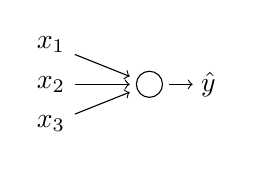
\begin{tikzpicture}
  \node (x1) at (0, 1) {$x_1$};
  \node (x2) at (0,.5) {$x_2$};
  \node (x3) at (0, 0) {$x_3$};
  \draw[->] (x1) to (1, .6);
  \draw[->] (x2) to (1, .5);
  \draw[->] (x3) to (1, .4);
  \node[draw=black,circle] (z) at (1.25, .5) {};  % \node (params) at (1, .9) {$w,b$};
  \draw[->] (1.5,.5) to (1.8, .5);
  \node at (2, .5) {$\hat y$};
\end{tikzpicture}
\vfill\null \columnbreak
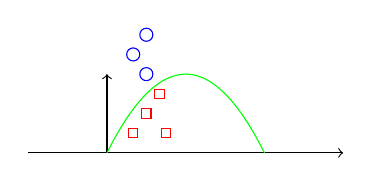
\begin{tikzpicture} \draw[->] (-1,0) -- (3,0) node[right] {};   
\draw[->] (0,0) -- (0,1) node[above]  {};
\draw[domain=-0:2,smooth,variable=\x,green] plot ({\x},{-(\x-1)^2 + 1});   
\node[draw=red, rectangle,scale=1/2] at (1/2, 1/2) {};
\node[draw=red, rectangle,scale=1/2] at (2/3, 3/4) {};
\node[draw=red, rectangle,scale=1/2] at (1/3, 1/4) {};
\node[draw=red, rectangle,scale=1/2] at (3/4, 1/4) {};
\node[draw=blue, circle,scale=1/2] at (1/2, 3/2) {};
\node[draw=blue, circle,scale=1/2] at (1/3, 5/4) {};
\node[draw=blue, circle,scale=1/2] at (1/2, 1) {};
\end{tikzpicture}
\vfill\null \columnbreak
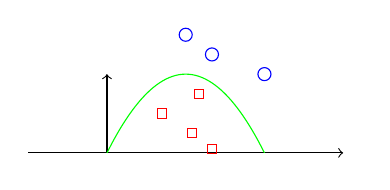
\begin{tikzpicture} 
\draw[->] (-1,0) -- (3,0) node[right] {};   
\draw[->] (0,0) -- (0,1) node[above]  {};
\draw[domain=-0:2,smooth,variable=\x,green] plot ({\x},{-(\x-1)^2 + 1});   
\node[draw=red, rectangle,scale=1/2] at (1/2+1/5, 1/2) {};
\node[draw=red, rectangle,scale=1/2] at (2/3+1/2, 3/4) {};
\node[draw=red, rectangle,scale=1/2] at (1/3+1, 1/4-1/5) {};
\node[draw=red, rectangle,scale=1/2] at (3/4+1/3, 1/4) {};
\node[draw=blue, circle,scale=1/2] at (1, 3/2) {};
\node[draw=blue, circle,scale=1/2] at (4/3, 5/4) {};
\node[draw=blue, circle,scale=1/2] at (2, 1) {};
\end{tikzpicture}
\end{multicols}
\end{minipage}

The idea behind covariate shift is that if we learned some $X \leadsto Y$ mapping, then if the distribution of 
$X$ changes we may need to retrain our learning algorithm. This remains true even if the ground truth function mapping $X \leadsto Y$ has remained static, as in our example above. Note that if the ground truth function \emph{also}
shifts, then the problem of covariate shift becomes even more acute.

\paragraph{Understanding batch-norm and how it enables learning between layers to be decoupled}
Consider a multiple-layer neural network. The job of an intermediary layer is to take the output activations from the layer prior and learn a mapping (through tuning weights $W, b$) from these inputs to $\hat y$. But because the output activations from the layer prior also depend on learned weights, the distribution can change quite drastically during training. What batch-norm does is effectively mitigate the amount of covariate shift from previous layers by 
ensuring that the input to the current layer has a fixed mean and variance. By limiting how updates in the network to earlier layers can affect the distribution of inputs to later layers, we cause the input values to later nodes of the network to become more stable and this really improves learning. So, even \emph{if} our input data does shift distribution, the learned parameters $\gamma, \beta$ in earlier layer will ensure that the values input to latter layers remains more stable. From the perspective of the latter layers, the inputs haven't shifted \emph{as} much. 
Put differently, we \emph{decouple} learning between layers, allowing each to learn by itself. 

\paragraph{Unintended side-effect: regularization}
Another interesting note is that batch-norm can be viewed as a form of regularization. To see this, first understand
that in each mini-batch $X^{\{t\}}$ of data we process, the values $z^{[\ell]}$ are re-scaled based only on $X^{\{t\}}$
 which may only consist of 64, 128, or 256 examples. So, our calculations for mean and variances are a little 
bit noisy as a result, and this in turn means that our scaling process of going from $z^{[\ell]}$ to $\tilde z^{[\ell]}$ is also a bit noisy. By adding some noise to inputs of hidden units, its forcing downstream hidden units not to rely too much on any one hidden unit. Similar to dropout, it adds noise to the hidden layers and therefore has a slight regularization effect. Note that if we choose a larger mini-batch size, our estimates for $\mu$ and $\sigma^2$ become more stable and the effect of regularization is reduced. This all said, the primary intent of batch-norm is to 
speed up training, not to encourage regularization.

\subsubsection{Batch-norm at Test time} Batch-norm processes our data one mini-batch at a time. But, at test time
we might need to process examples one at a time. How can we adapt our network to do that? Recall that during training,
we use the following equations to implement batch-norm; we use $m$ to denote the number of examples in the mini-batch (\emph{not} the whole training set).
\begin{align}   \mu &= \frac{1}{m}\sum_{i=1}^m z^{(i)} \nonumber \\
  \sigma^2 &= \frac{1}{m} \sum_{i=1}^m \left(z^{(i)} - \mu\right)^2 \nonumber \\
  \label{eq: zinorm}
  z^{(i)}_{\texttt{norm}} &= \frac{z^{(i)} - \mu}{\sqrt{\sigma^2 + \epsilon}} \\
  \tilde z^{(i)} &= \gamma z^{(i)}_{\texttt{norm}} + \beta \nonumber \end{align}

Notice that $\mu, \sigma^2$ are both computed on the entire mini-batch. But at test time, we may not have a mini-batch
of size 64, 128, or 256 examples to process at a time. What's actually done? We come up with separate estimates of
$\mu, \sigma^2$ where we typically estimate these values using exponentially weighted averages across mini-batches.
To make this concrete, fix attention to some layer $\ell$. As we train our network on different mini-batches $X^{\{1\}}, X^{\{2\}}, X^{\{3\}}, \ldots$, we accumulate different estimates for $\mu^{\{1\}[\ell]}, \mu^{\{2\}[\ell]}, \mu^{\{3\}[\ell]}, \ldots$. The exponentially weighted averages across mini-batches informs us of our estimate for $\mu$. Similarly for $\sigma^2$. So, as we train our neural network we accumulate a running average of these $\mu, \sigma^2$ parameters that we plan to use at test time. At test time, we modify \ref{eq: zinorm} to use our (exponentially weighted) estimates for 
$\mu, \sigma^2$. We still apply the learned parameters $\gamma, \beta$ learned at train time to re-scale our $z^{(i)}_{\texttt{norm}}$. Lastly, we remark that there are many ways we could go about estimating $mu, \sigma^2$ to apply at test time, but that the performance of a network does not typically hinge on these hyperparameters too much.

\subsection{Multi-class classification} 
\paragraph{Generalization of Logistic regression: Softmax regression}
So far, the examples we've used for classification have been 
\emph{binary}, where there are only two possible labels. For instances where there are multiple possible classes,
there is a generalization of logistic regression called \href{https://en.wikipedia.org/wiki/Softmax_function}{Softmax} regression. Denote by $C$ the number of classes we are trying to categorize our inputs into. We index into our classes from $\{0, 1, \ldots, C-1\}$. The goal is to build a new neural network where the output layer has $C$ units. We'd like for the output units to inform us of the probability of belonging to the corresponding class. To be explicit, in Python notation our output vector is now $(C, 1)$ dimensional.

\paragraph{Multiple neurons in output layer}
In the final layer of our network with $C$ nodes, each node still consists of two parts: a linear mapping and a non-linear mapping. We still compute $z^{[L]} = W^{[L]} a^{[L-1]} + b^{[L]}$, and once we have this we can now feed it into a Softmax activation function. The first step is to compute a temporary variable $\texttt{tmp} = e^{z^{[L]}}$ where the exponential function is applied element-wise. Then, the output for the final layer is given by
\[
a^{[L]} = \frac{e^{z^{[L]}}}{\sum_{j=1}^C \texttt{tmp}_j}.
\]
\paragraph{Output layer yields a probability distribution}
In other words, each element $a_i^{[L]} = \frac{\texttt{tmp}_i}{\sum_{j=1}^C t_j}$ is an element of a probability 
distribution since we've (i) mapped the real number line to the positive half-space and then (ii) 
performed normalization by a sum such that the elements add to unit value. The unusual thing about the 
Softmax activation function is that it takes as input a real vector and outputs a real vector, as opposed to our 
previous activation functions which are scalar valued. One important aspect of a Softmax classifier is 
that the decision boundary between any two classes is linear, 
so if we don't use any non-linear transformations in our hidden layers then we will end up with a linear decision boundary between classes.

\subsubsection{Training a Softmax classifier} Notice that the Softmax function maps the largest input value to the largest probability element. This is analagous to a hardmax function, which for a given vector $(x_1, \ldots, x_n)$,
emits a binary vector of equal length consisting of all zeros except for the position corresponding to the maximum input, which consists of a unit value. E.g. hardmax would map $\begin{bmatrix}   12 & 4 & -3 \end{bmatrix}$ to $\begin{bmatrix}   1 & 0 & 0 \end{bmatrix}$.

\paragraph{Loss and cost function} Let's consider our loss function for multi-class classification.
\begin{equation}
\label{eq: multiclassloss}
\mathcal L (\hat y, y) = -\sum_{j=1}^C y_j \log \hat y_j.
\end{equation}
We can see why this makes sense on a toy example. Suppose we have our multi-class output layer ground-truth $y = \begin{bmatrix}
0 & 1 & 0 & 0 \end{bmatrix}$, i.e. this is an example of the second class. Then notice that $y_1 = y_3 = y_4 = 0$, and our 
loss function \ref{eq: multiclassloss} reduces to $-y_2 \log \hat y_2 = -\log \hat y_2$. Since we wish to minimize our
loss function, this is equivalent to making $\hat y_2$ really large, i.e. we want to emit a large probability for this
label. What about our \emph{cost} function? It's what you'd expect:
\[
J(W^{[1]}, b^{[1]}, \ldots) = \frac{1}{m} \sum_{i=1}^m \mathcal L(\hat y^{(i)}, y^{(i)}).
\]

\paragraph{Dimensions of output}
Let's clarify our dimensions. We have $Y = \begin{bmatrix}   y^{(1)} & y^{(2)} & \ldots & y^{(m)} \end{bmatrix}$ where each $y^{(i)}$ is $(C, 1)$ dimensional. So, $Y, \hat Y \in (C, m)$.

\paragraph{Backpropagation and gradient descent with Softmax} The key equation is that $\frac{\partial J}{\partial z^{[L]}} = \d z^{[L]} = \hat y - y$ which is a $(C, 1)$ dimensional vector.

\section{Structuring Machine Learning Projects}
\subsection{Introduction to ML Strategy}
\paragraph{Why ML Strategy?} Suppose you're working on a cat classifier, which in spite of having 90\% accuracy
is not good enough for your application. You start to brainstorm ideas: collect more data, collect more diverse 
data, train the algorithm longer, or try a different algorithm, or we could also think about network sizes (either smaller or bigger), trying dropout, adding $\ell_2$ regularization, rewiring the network architecture including
activation functions and the \# of hidden units. What if we spend 6 months acquiring more training data, only to realize that it barely helps our model? Wouldn't it be nice if we could know which techniques are worthwhile and which
we can safely discard? This course is about strategy, motivated by practical learnings from Andrew Ng. 

\subsubsection{Orthogonalization} There are many hyperparameters we can tune.Orthogonalization is the notion of being clear-eyed about what exactly we're tuning in order to have a particular desired effect. Consider as an example an old-school television set, with many knobs. One enlarges the picture vertically, another horizontally, another controls 
how trapezoidal the image appears, whilst others allow vertical and horizontal translation as well as rotation. It's an important UI/UX feature that each knob controls an interpretable function. Imagine how hard it would be to tune a
television where the first knob controls a linear combination of the adjusters we listed above (e.g.
$0.1 \times \texttt{height} + 0.3 \times \texttt{trapezoidal} + \ldots$). 

In the context of the television designers,
orthogonalization refers to designing each knob to achieve a single outcome. This makes it easier to tune the television and center the picture. Another example could be in the context of a car: we have a steering wheel to control left-and-right direction, as well as a gas and brake pedal to control speed. Theoretically, if we had a joystick that controlled $0.3 \times \texttt{steering\_angle} - 0.8 \times \texttt{speed}$ and another joystick which controlled 
$2 \times \texttt{steering angle} + 0.9 \times \texttt{speed}$, this would suffice to control the car however we'd like. But it's much harder to control than if we had separate controls for each function. 

\paragraph{We tune knobs to satisfy the following four conditions}
For a supervised learning system, we'd like to tune knobs so that the following hold true:
performance is acceptable on the training set (perhaps relative to human level performance), 
the development set, the test set, and finally we'd like for our cost
function when applied to the test set to correlate well with real world performance.
\begin{enumerate}   \item If we're not fitting to the training set well on the cost function, we might train a bigger network, or a better optimization algorithm like Adam.
  \item If we're not fitting well on the development set but it is on the training set, we might consider a set of knobs around regularization or getting a larger training set.
  \item If we're not fitting well on the test set but we are on the development set, it probably means the development set was too small (i.e. we've overfitted to it) and so we need to acquire a larger development dataset.
  \item If we're not performing well in the real world but we are on the test set, then we need to go back and change either the development set or the cost function. \end{enumerate}

One example of a knob that is \emph{not} orthogonalized is \emph{early-stopping}: this is an operation that simultaneously affects performance on training set (stopping early you fit the training set less well) but its often intended to improve performance on the development set.

\subsection{Setting up your goal}
\paragraph{Single (real) number evaluation metric} Progress will be much faster if you have a single real number evaluation metric which lets you tell if your new idea is making an improvement (or not). As a motivating example, consider
a cat classifier; it's reasonable to examine both precision (the percentage of predictions labeled as cats that actually are cats) and recall (the percentage of the cat population that was correctly classified as a cat). There is often
a tradeoff between precision and recall, and it turns out we'd like to have both: when the classifier says something
is a cat, we'd like there to be a high chance of this being true, but similarly for all the images of cats we'd want
our classifier to correctly label most of them as cats as well. Having
two real numbers makes it tough to evaluate many different models against each other. In machine learning, it's traditional to combine both of these metrics into an \href{https://en.wikipedia.org/wiki/F1_score}{F1 score}, which is the \href{https://en.wikipedia.org/wiki/Harmonic_mean}{harmonic mean} of \href{https://en.wikipedia.org/wiki/Precision_and_recall}{precision and recall}.
\[
F_1 = \frac{2}{\texttt{recall}^{-1} + \texttt{precision}^{-1}} = 2 \cdot \frac{\texttt{precision} \cdot \texttt{recall}}{\texttt{precision} + \texttt{recall}}.
\]
 
\paragraph{Satisficing and Optimizing Metrics} 
What if we're considering not only the accuracy of a classifier, but also its cost in compute time? It might seem artificial to come up with a linear combination of these metrics in order to derive a single real number, e.g. \texttt{accuracy - 0.5 x runningTime}. Instead, we might decide that we'd like to \emph{maximize} accuracy \emph{subject to}
the latency of our algorithm being below some threshold. Then, we say that accuracy is an optimizing metric and
 latency is a satisficing metric.

If we have $N$ metrics we really care about, Andrew recommends making one of them an optimizing metric and
the reamining $N-1$ satisficing.

\paragraph{Train/dev/test distributions} Note that the development set is 
sometimes called the cross-validation dataset in other literatures. The core workflow in machine learning is
\begin{itemize} \item Try a lot of ideas by training different models on the \emph{train}ing set.
\item Use the development set to evaluate the different ideas and select one.\footnote{Andrew states that it's permissible to keep innovating by improving development set performance.}
\item Evaluate the efficacy of your approach via the test set. \end{itemize}

It's critical that the development and test sets come from the same distribution. As an example, consider training a classifier to predict the likelihood of a loan application being processed on data restricted to \emph{medium} income
postal codes; such a classifier may not perform well at all when evaluated on data drawn from \emph{low} income
postal codes.

\paragraph{Size of development and test sets} We've emphasized that development and test sets should come from the same distribution. But how large should they be? In the past when datasets were smaller, using a rule of thumb like
allocating 60/20/20 for train/dev/test was reasonable. But modern datasets are so large that it might be quite reasonable to allocate 98\% for training, and another 1\% for development and test each. Since many algorithms have an appetite for data, it's reasonable to allocate more toward training. Remember as well that the purpose of the test set is simply to get an unbiased estimate of error; unless you need to have a very accurate measurement of how your final system is performing, you might not need millions (and millions) of examples but instead maybe 10-100k. It's worth noting that the size of the development set must be large enough that we overfit to it.

\paragraph{When to change dev/test sets and metrics} Sometimes, partway through a project you realize you may have
set up your dev/test sets incorrectly; in this case, you should move your target accordingly. Consider two cat classifiers where one has slightly lower test error than another but allows pornographic images to also be shown to users.
This would be totally unacceptable, and so in light of this we might want to change either our dev/test sets or our
evaluation criterion. Suppose we define error as $\frac{1}{m_{\texttt{dev}}} \sum_{i=1}^{m_{\texttt{dev}}} \mathbbm 1_{\{\hat y^{(i)} \neq y^{(i)}\}}$, then we may wish to modify our criterion for error to instead be something like
\begin{align*}   & \hspace{10pt} \frac{1}{\sum_{i=1}^{m_{\texttt{dev}}} w^{(i)}} \sum_{i=1}^{m_{\texttt{dev}}} \color{orange}{w^{(i)}} \color{black} \mathbbm 1_{\{\hat y^{(i)} \neq y^{(i)}\}}, \textrm{ where } \\
  w^{(i)} &= \begin{cases}     1 & \textrm{if } x^{(i)} \textrm{ is non-pornographic} \\
    100 & \textrm{if } x^{(i)} \textrm{ is pornographic}   \end{cases} \end{align*} where we've added weights to properly penalize presenting a pornographic 
image and we've also updated our loss function's normalization constant such that error lies in the unit interval.
Recall the concept of orthogonalization: we (i) define a metric that captures we'd like to achieve and then (ii) 
worry about how to optimize over that metric. One example of when to change dev/test sets is if we're training an image classifier on professional photographs but users are interfacing with our model by providing as inputs more blurry
and less focused photos; we might consider switching dev/test sets in this case.

\subsection{Comparing to human-level performance}
A lot more machine learning teams are starting to compare their performance to that of what humans can achieve.
There are two main reasons: (i) advances in deep learning mean that it's actually feasible for an algorithm to
achieve human level performance, and (ii) the workflow of designing and building a machine learning system is more 
efficient when you're trying to emulate something a human can also do. In these settings, it becomes natural to compare the performance of an algorithm with a human (figure \ref{fig: progress-over-time}).
\begin{figure}[h]
  \centering   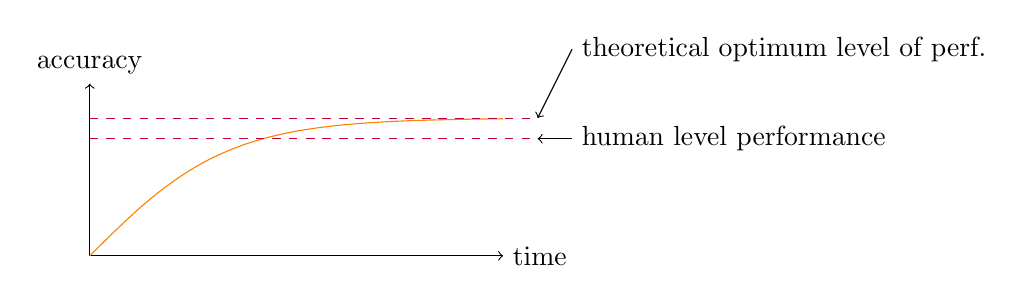
\begin{tikzpicture}[scale=1.75]     \draw[->] (0,0) -- (3,0) node[right] {\textrm{time}};   
    \draw[->] (0,0) -- (0,1.25) node[above] {\textrm{accuracy}};
    \draw[domain=0:3,smooth,variable=\x,orange] plot ({\x},{(tanh(\x))});     \draw[domain=0:3.25,smooth,variable=\x,purple, dashed] plot ({\x},{1}); 
    \draw[domain=0:3.25,smooth,variable=\x,purple, dashed] plot ({\x},{0.85}); 
    \draw[<-] (3.25, 1) -- (3.5, 1.5);
    \draw[<-] (3.25, 0.85) -- (3.5, 0.85);
    \node at (3.5, 1.5) [right] {\textrm{theoretical optimum level of perf.}};
    \node at (3.5, 0.85) [right] {\textrm{human level performance}};
  \end{tikzpicture}
  \label{fig: progress-over-time}
  \caption{A typical plot of progress on a problem within a machine learning team. Progress is rapid until
    human level performance is surpassed, at which point progress may still continue but at a slower rate.
    Eventually and in an ideal world, performance of an algorithm approaches the theoretical upper bound on 
    performance which is dictated by the Bayes error rate.} \end{figure}

It's important to emphasize that no matter how hard you work on a problem, you can never surpass \href{https://en.wikipedia.org/wiki/Bayes_error_rate}{Bayes error rate}, and further no human can outperform Bayes error 
rate by definition.\footnote{An algorithm only outperforms the Bayes error rate on a training dataset if its overfitting.}
But it also turns out that progress is quite fast until human level performance is surpassed. Why is this?  One reason
is that for many tasks, human level performance is not that far off from Bayes optimal error, i.e. people are very 
good at various tasks. But a more fundamental reason is that tools that can help improve model accuracy that are available to use for models performing below human level performance become intractable to use when the model has surpassed human level performance. Specifically, so long as your machine learning algorithm is performing worse than what humans, you can higher humans to create labeled data to feed your algorithm. By asking raters to classify inputs that your
algorithm is likely to get wrong, you (or your algorithm) can gain an insight as to where you went wrong; this helps
to improve model performance. Once your algorithm starts outperforming humans, this option is no longer efficacious.

\paragraph{Avoidable bias} Sometimes, understanding how accurately humans can perform a task can inform us of whether
we should focus on reducing bias or variance in our model. For example, suppose we have a task of classifying whether
a cat is in an image. Perhaps a human error rate is 1\%, but our model shows 8\% error on development set and 10\% on
the test test; in this case, we'd like to focus on reducing the bias of our algorithm by training a larger network,
or running our training algorithm longer (the point is to focus on 
things that increase performance on the \emph{training} set). But what if the input images are really blurry and
humans can only achieve a 7.5\% error rate?  In this case we might be wise to focus on reducing the variance of our algorithm, e.g. trying regularization or getting more training data to close the gap between dev/test error. Andrew coins the gap between Bayes error and training error to be \emph{avoidable bias}.
\begin{equation*}   \texttt{AvoidableBias} = \texttt{BayesError} - \texttt{TrainingError}. \end{equation*}

\paragraph{Understanding human-level performance} How can we define the phrase ``human-level performance'' more 
precisely? We'll start with an example of medical image classification: given a radiology image make a diagnosis 
decision; suppose an untrained human achieves 3\% error, a doctor 1\% error, an experience doctor 0.7\% error, and a panel of doctors who discuss the image by committee can earn a 1/2\% error. The question becomes, which benchmark serves as human level performance? We know that Bayes error is less than or equal to 1/2\%, and since we like to proxy Bayes error by human level performance, it makes sense to say that human level performance is 1/2\% in this example. But it also could be the case that for the purpose of deploying a system in practice, that we'd only need to outperform a typical doctor; this could be a very useful result if accomplished and so in some cases it could make sense to argue toward defining human level performance as 1\% in the example above. The point is that we should be clear about what our intentions are when defining human level performance: is it to approximate Bayes error or is it to put a machine learning system into deployment?

So, to summarize, when we consider the bias-variance problem(s) and which to focus on first, it's important to compare
training set error not with 0\% error rate but with Bayes error rate or a proxy thereof, via human-level performance.
Then, once we have an idea of the magnitude of avoidable bias as well as the difference between dev/test error, we can
choose the larger problem to focus our efforts on.

\paragraph{Surpassing human-level performance} What happens if an algorithm outperforms a team of human experts working together, and simultaneously achieves low dev/test error gap? Here, it's not obvious whether to focus on the bias or variance problem, since we have no estimate for Bayes error: we simply know that it's at or below what our model is performing on the development (and test) sets. What are some example problems where ML has significantly surpassed human-level performance? Some instances are in online advertising (estimating likelihood of a person clicking an ad), another is product recommendations, logistics (predicting transit times), or loan approvals. It's noteworthy that all
these datasets are based on structured data, and none of the problems are based on \emph{natural perception}
tasks such as computer vision or natural language processing. Lastly, each of the examples where algorithms surpass human level performance have enjoyed massive amounts of data. 

\paragraph{Two fundamental assumptions of supervised learning}
\begin{enumerate}   \item You can fit the training set pretty well (avoidable bias).
  \item The training set performance generalizes pretty well to the dev/test set. \end{enumerate}
To improve the performance of an ML system, first get a notion of avoidable bias
by looking at the difference between human-level performance and training error.
Then, get a notion of magnitude of the variance problem by examining the difference
between dev/test error. To reduce avoidable bias, tactics like training larger models, training longer, using a better optimization algorithm, or even rewiring the network architecture.  If variance is a problem, you can get more training data (to help generalize to dev/test sets), regularization ($\ell_2$, dropout, data augmentation), or rewiring the network architecture. 

\subsection{Error Analysis} Suppose you are trying to get a learning algorithm to accomplish what a human can,
but your algorithm has not yet achieved human level performance. Then, inspecting mistakes that your algorithm
has made can give insight into what to do next; this process is known as error analysis.

\paragraph{Carrying out error analysis} Suppose you have a hunch that your classifier is making a particular type
of mistake that you can envision fixing with diligent effort. The question becomes is it possible to know in advance
whether it's ``worth it'' to embark on such a project. An error analysis might consist of getting 100 mislabeled
development set examples, and counting how many are attributable to the type of mistake you're interested in.
This yields an upper bound on how much performance could be improved if we were to correctly classify these examples. In just a few minutes, this gives an estimate of whether its worth tackling a particular type of problem.

\begin{table}[h]
\centering \begin{tabular}{c|c c c | c}
Image & Dog & Great Cats & Blurry & Comments \\
\hline
1 & \checkmark & & & Pitbull \\
2 & & & \checkmark & \\
3 & & \checkmark & \checkmark & Rainy day at zoo\\
$\vdots$ & $\vdots$ &$\vdots$ &$\vdots$ & \\
\hline
\% of total \end{tabular}  
\caption{Often, we have multiple ideas for how to improve an algorithm. Andrew recommends making a spreadsheet tracking the
error analysis for each idea in parallel; e.g. the table above.
The conclusion of this process informs us where to direct our efforts, as well as upper bounds for how much we can
expect to improve performance.} 
\end{table}

\paragraph{Cleaning up incorrectly labeled data}
A supervised learning problem comprises of a mapping $X \leadsto Y$.
Suppose we dig through our data and find that some output labels in $Y$ are incorrect.
Is it worth your time to fix some of these labels? Note that we make a semantic distinction here:
an algorithm that doesn't predict the right label is said to \emph{mislabel} an example, but an example
that is incorrectly marked in the (training/dev/test) data itself is said to be an \emph{incorrect} label

If the errors are reasonably random it's not worth worrying about as learning algorithms tend to be robust to random errors.
So long as the total dataset size is large enough, and the actual percentage of incorrectly labeled examples is not \emph{too} high,
it's probably not worth your time to fix the mistakes. If the errors are systematic it's a different story. Andrew recommends proceeding with an error analysis as described above, by adding a column counting the number of incorrect labels among mislabeled predictions, so that we can estimate an upper bound on the benefit we'd get from fixing the labels ourselves.

If you do decide to correct labels in your dev set, you should apply the same procedure to your test set and at the same time. This
is in order to preserve the similarity in distribution between the two datasets. That said, we don't always need to apply the same
procedure to the training data, for several reasons: the training data are much larger and so this can be a much more onerous task, and learning algorithms can handle cases where they are trained on data from a slightly different distribution than what they are evaluated on (so long as dev/test are consistent, our estimates for which algorithm is best and its performance are unbiased).

\paragraph{Build your first system quickly, then iterate} This is a piece of advice from Andrew 
that applies less if (i) you have significant domain experience or (ii) there is a body of academic literature
you can draw upon that addresses the same problem. 
Suppose you're building a speech recognition system: there are many directions you could go in terms of how to prioritize 
improvements. E.g. you would focus on
\begin{itemize}[topsep=2pt,itemsep=0.5pt,partopsep=1pt,parsep=1pt]
  \item Noisy backgrounds (where in fact caf\'e noise is different from car noise),
  \item Accented speech, for which there are particular ways to make the recognition system more robust,
  \item Far from microphone (known as far-field speech recognition),
  \item Young children's speech (how they pronounce words, and which words are used), or
  \item Stuttering (and how to handle nonsensical phrases like ``oh'', ``ah'', ``um''). \end{itemize}
It's not obvious where to focus your efforts. Instead, build quickly then iterate: set up a dev/test set and
a metric, then build an initial machine learning system and train it. The key is to
\begin{enumerate}[topsep=2pt,itemsep=0.5pt,partopsep=1pt,parsep=1pt] \item Understand performance on dev/test, 
\item Apply corresponding bias-variance analysis, and lastly
\item Set up an error analysis \end{enumerate}
in order to prioritize next steps. By having first built a quick-and-dirty system, 
we can now \emph{localize} the problem: e.g. does the error
analysis inform us that far-field speech recognition techniques could greatly benefit our performance?

\subsubsection{Mismatched Training and Dev/Test Set} Deep learning algorithms have a huge hunger for 
labeled training data. Sometimes, teams are tempted to throw more and more training data at an algorithm
in spite of it not coming from the same distribution as their dev/test set; there are some subtleties
in how we can deal with this.

\paragraph{Training and testing on different distributions} Suppose you're building a mobile application whereby users will
upload photos taken from cell phones, and you'd like to recognize whether the photograph contains a cat. For the sake of simplicity,
suppose there are two main sources of data you can obtain: (i) the distribution of data you really care about, which tends to be
less professionally shot, less well-framed, and perhaps even blurrier because it is shot by amateur users, or (ii) crawling the web
and downloading a lot of professional, high-resolution, and well-framed cat photographs. Perhaps our mobile app doesn't yet have
a lot of users, and so we have 10,000 photographs from our app but crawling the web gets us another 200,000 images.

What we care about in the end is how well our algorithm performs on the set of images drawn from the mobile phone 
distribution, because in the end that's how our users will upload their photos. But you don't \emph{just} want to train
on 10,000 images, because that's just perhaps too small a training set. One thing we could do, is take \emph{all} of the 210,000
images we have (drawn from different distributions) and shuffle them into train/dev/test sets. There are advantages and disadvantages to this approach. The advantage is that your train/dev/test sets all come from the same distribution. But, the (huge) disadvantage
is that our dev set is likely to contain a disproportionate amount of professional photographs relative to mobile uploads. In expectation, $\frac{200}{210} \times 100 \%$ of our development set will come from professional photographs, and only $\frac{10}{210} \times 100\%$ will come from mobile uploads. Therefore, Andrew recommends \emph{against} this option of randomly shuffling our data together.

Instead, we can still use the same number of images in the training set: we'll use \emph{all} of the data drawn from the distribution we \emph{don't} care about in addition to some of the data we \emph{do} (e.g. we'll use 200,000 professional images from the web and another 5,000 from our mobile phone uploads) and then the dev/test shall consist \emph{only} of images that we actually care about (e.g. the remaining 5,000 mobile phone uploads). The advantage of this method is we're now being more precise in how we specify
our dev/test set performance and how it relates to real-world performance. The disadvantage is that the distribution of our
\emph{training} data is different from that of dev/test. However, this split of data yields better performance in the long term.

Let's consider a second example. Suppose we're building a speech recognition system which replaces a rear-view mirror in a car into
a smart-device. Perhaps we've worked on speech recognition before, and we have a lot of data from other speech recognition applications but not from a \emph{speech-activated rear-view mirror}. Our training set shall consist of all speech recognition data we've
accumulated over the years (which comes in $(x,y)$ pairs where $x$ is an audio-clip and $y$ is a transcript), perhaps this includes
smart voice activated speakers, keyboards, etc. But crucially, \emph{our} rear-view mirror application will involve a lot more
\emph{navigation} requests because the device is situated in a car. Therefore, 
the distribution of our dev/test sets shall be drawn from speech activated rear-view mirrors, and will be different from our 
training data which will consist of all other data.\footnote{Perhaps if we don't think we need \emph{all} the speech-activated rear-view mirror examples in our dev/test sets (i.e. they are already sufficiently large), then we can place some examples in our training set.}

\paragraph{Bias and variance with mismatched data distributions} Estimating the bias and variance of your learning algorithm
can greatly inform what to prioritize next. But the way you analyze bias and variance changes when your training set is drawn from a different distribution than your dev/test set. Suppose we're in the realm of cat classification for images, and so Bayes optimal error is nearly zero. To carry out bias-variance analysis, we typically examine training error in conjunction with error on the dev set. Suppose training error is 1\% and development set error is 10\%. \emph{If} your training and development sets are drawn from the \emph{same} distribution, then you have a variance problem and that our algorithm is not generalizing well from the training set. However, if the data are drawn from different distributions this is no loner a safe conclusion: perhaps the development set is just much harder to classify on. The problem with this analysis was that as we changed from looking at training error to dev error, two things changed at one time: (i) the algorithm saw data in the training set but not the dev set, and (ii) the distribution of dev data 
is different. Because we changed two things at a time, it's difficult to know if the 9\% increase in error is due to the algorithm
not having seen the examples before (part of the variance problem) \emph{or} if its just because the dev set data is different.

In order to tease out these differences, we'll define a new piece of data called the \texttt{training-dev} set. This will be a new
subset of data that we carve out which will have the \emph{same} distribution as our training data \emph{but} we will \emph{not}
explicitly train our network on this data. So, to be explicit: the setting is that our dev/test sets are drawn from the same distribution but our training set is drawn from a different distribution. We'll take a partition our training data with a smaller piece 
going to the \texttt{training-dev} set, so now just as the dev/test sets have the same distribution so do the training data alongside the \texttt{training-dev} set. To carry out error analysis, you should now look at misclassified examples from \emph{each} of
the training set, the \texttt{training-dev} set, \emph{and} the development set.

Suppose we have 1\% training error, 9\% \texttt{training-dev} error, and 10\% dev set error. We can \emph{now} conclude that we have a large variance problem, since all that changed when moving from measuring error on training set to the \texttt{training-dev} set
was that our network hadn't yet seen the examples (but the distribution remained the same). So, our network isn't generalizing well
to examples drawn from the same distribution.

Suppose as a different example that we have a 1\% training error, a 1.5\% \texttt{training-dev} error, but when we go to the development set we get a 10\% error. Now, our variance problem is relatively low: the error only increased slightly in moving to unseen examples drawn from the same distribution. What we have here is a data mismatch problem.

Suppose as another example the training error is 10\%, \texttt{training-dev} is 11\%, and development set error is 12\%. Here, our largest problem is \emph{avoidable bias}, since our proxy for Bayes optimal error is zero in the cat classifying example. As a last example, suppose training error is 10\%, \texttt{training-dev} error is 11\%, and dev error is 20\%. Here, we have two issues: the avoidable bias is high, and although the variance problem is small (difference between \texttt{training-dev} and training error is small), there is a large discrepancy between \texttt{training-dev} and development set error which indicates a data mismatch problem.  

\begin{figure}[h]
\centering
\label{fig: relationshipsbwdifferrs}
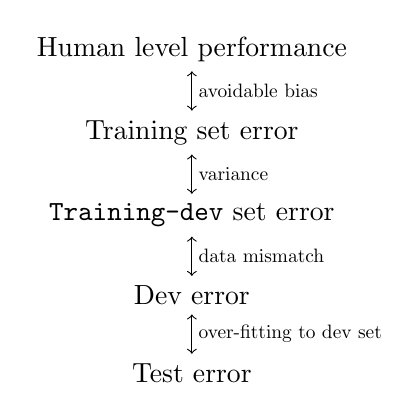
\begin{tikzpicture}   \node (hlp) at (0, 0) {\textrm{Human level performance}};
  \node[below = 0.5 cm of hlp] (train) {\textrm{Training set error}}; 
  \draw[<->] (hlp) -- (train) node[midway,right,scale=0.7] {\textrm{avoidable bias}};
  \node[below = 0.5 cm of train] (traindev) {\textrm{\texttt{Training-dev} set error}};
  \draw[<->] (train) -- (traindev) node[midway,right,scale=0.7] {\textrm{variance}};
  \node[below = 0.5 cm of traindev] (dev) {\textrm{Dev error}};
  \draw[<->] (traindev) -- (dev) node[midway,right,scale=0.7] {\textrm{data mismatch}};
  \node[below = 0.5 cm of dev] (test) {\textrm{Test error}};
  \draw[<->] (dev) -- (test) node[midway, right,scale=0.7] {\textrm{over-fitting to dev set}}; \end{tikzpicture}
\caption{The relationship between different types of data and the problems we may run into when there are measurable gaps in error between adjacent levels.}
\end{figure}

Andrew also cautions that it's possible for the dev/test error to be lower than that of our training error or our \texttt{training-dev} error. Consider the following table which generalizes the above analysis:
\begin{table}[h]
\centering
\begin{tabular}{c| c c }
 & $\substack{\textrm{General speech} \\ \textrm{recognition}}$ & $\substack{\textrm{Rearview mirror} \\ \textrm{speech data}}$ \\
\hline
Human level & ``Human level'' & \\
$\substack{\textrm{Error for} \\ \textrm{output trained on}}$ & ``Training error'' & \\
$\substack{\textrm{Error for} \\ \textrm{examples \uline{not}} \\ \textrm{trained on}}$ & ``\texttt{Training-dev} error'' & ``Dev/test error''\\ \end{tabular}
\end{table}

We've seen the relationships between filled in entries in figure \ref{fig: relationshipsbwdifferrs}. If we fill in the remaining missing entries, we can sometimes gain additional insights such as, ``if human level performance varies from one problem to another, then its indicative one problem may be \emph{harder} than another''. Or, we can understand bias-variance and data mismatch problems in different degrees.

\paragraph{Addressing data mismatch} What if your training set comes from a different distribution than your dev/test sets, and furthermore your error analysis shows that you have a data mismatch problem. What can you do? Andrew recommends carrying out a \emph{manual} error analysis and trying to understand the differences between the training set and the dev set.\footnote{We remark that to avoid overfitting to your test set, for the sake of error analysis you should only manually inspect the development set.} E.g. in
the context of the speech-activated rear-view mirror application, you might listen to examples in your development set to try
and figure out how they're different from your training set: perhaps car noise is a problem that arises, or mis-classification of
numbers involved in the parsing of street numbers. Once you've identified how the development set may be harder than the training
set, you can look into ways to making the training set more similar, or perhaps collect more data that is similar to your dev/test
sets. E.g. you could simulate noisy in-car data, or you could get more data of people speaking out numbers. 
These are rough guidelines, and not systematic recommendations.

\paragraph{Artificial data synthesis}
If the goal is to make your training data more similar to your development set, one technique you could use is artificial data synthesis. In the context of the car noise problem, this could mean taking clean (background noise-free) audio examples and super-imposing them with background car noise to generate a new example. This simple audio synthesis can create more data that is more similar to your dev/test distribution. There's one caveat: suppose you have 10k hours of clean audio but only 1 hour of car noise. If we naively re-apply this one hour of car noise to all 10k hours of clean audio, our learning algorithm may over-fit to this particular
type of background noise. You could imagine that our synthesized data only simulates a very small subset of the space of all possible audio clips with background car noise.

As another example, consider self-driving cars and the sub-problem of car detection (or drawing bounding boxes around cars within still images). Some people have thought before: can we render computer generated graphics (possibly from video games) to generate additional data? The problem is that our rendered simulation may only cover a small subset of the possible space of all cars and graphics that are required by a real application. I.e. to the human eye a video game simulation with 20 unique cars may look very realistic and as though we aren't running into repeat cars and designs, but a neural network may very quickly learn to overfit to this small subset of the space of data.

\subsection{Learning from Multiple Tasks} One of the most powerful ideas in deep learning is that you can sometimes take
knowledge learned by a neural network from one task, and apply that (part of that) knowledge to a separate task; this is called 
\href{https://en.wikipedia.org/wiki/Transfer_learning}{transfer learning}. Suppose as an example that you've trained your neural
network on image recognition, where $(x,y)$ pairs where $x$ is an image and $y$ is some object (e.g. a dog, cat, bird, etc.). Suppose we're interested in adapting this neural network to make a diagnosis in radiology.

\begin{figure}[h]
\centering
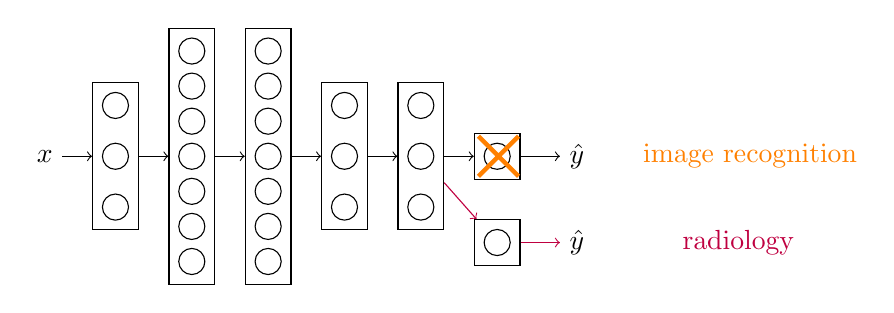
\begin{tikzpicture}[darkstyle/.style={circle,draw,fill=gray!40,minimum size=20}]
  \node (x) at (0, 0) {$x$};
  \node[draw, circle, right = 0.5cm of x] (l10) {};
  \node[draw, circle, above = .3cm of l10] (l11) {};
  \node[draw, circle, below = .3cm of l10] (l12) {};
  \node[draw, fit = (l10) (l11) (l12)] (layer1) {};
  \draw[->] (x) to (layer1);
  \node[draw, circle, right = 0.5cm of layer1] (l20) {};
  \node[draw, circle, above = .1cm of l20] (l21) {};
  \node[draw, circle, above = .1cm of l21] (l22) {};
  \node[draw, circle, above = .1cm of l22] (l23) {};
  \node[draw, circle, below = .1cm of l20] (l24) {};
  \node[draw, circle, below = .1cm of l24] (l25) {};
  \node[draw, circle, below = .1cm of l25] (l26) {};
  \node[draw, fit = (l23) (l26)] (layer2) {};
  \draw[->] (layer1) to (layer2);  
  \node[draw, circle, right = 0.5cm of layer2] (l30) {};
  \node[draw, circle, above = .1cm of l30] (l31) {};
  \node[draw, circle, above = .1cm of l31] (l32) {};
  \node[draw, circle, above = .1cm of l32] (l33) {};
  \node[draw, circle, below = .1cm of l30] (l34) {};
  \node[draw, circle, below = .1cm of l34] (l35) {};
  \node[draw, circle, below = .1cm of l35] (l36) {};
  \node[draw, fit = (l33) (l36)] (layer3) {};
  \draw[->] (layer2) to (layer3);  
  \node[draw, circle, right = 0.5cm of layer3] (l40) {};
  \node[draw, circle, above = .3cm of l40] (l41) {};
  \node[draw, circle, below = .3cm of l40] (l42) {};
  \node[draw, fit = (l40) (l41) (l42)] (layer4) {};
  \draw[->] (layer3) to (layer4);
  \node[draw, circle, right = 0.5cm of layer4] (l50) {};
  \node[draw, circle, above = .3cm of l50] (l51) {};
  \node[draw, circle, below = .3cm of l50] (l52) {};
  \node[draw, fit = (l50) (l51) (l52)] (layer5) {};
  \draw[->] (layer4) to (layer5);
  \node[draw, circle, right = 0.5cm of layer5] (fnode) {};
  \node[draw, fit = (fnode)] (fnodebox) {};
  \draw[->] (layer5) to (fnodebox);
  \node[right = 0.5cm of fnodebox] (yhat) {$\hat y$};
  \draw[->] (fnodebox) to (yhat);
  \node[right = 0.5cm of yhat] (imagerecog) {\color{orange} \textrm{image recognition}};
  \node[draw, ultra thick, orange, right = 0.435cm of layer5, cross out, scale = 1.75] {};
  \node[below = 0.75cm of fnode, draw, circle] (newnode) {};
  \node[draw, fit = (newnode)] (newnodebox) {};
  \draw[->, purple] (layer5) to (newnodebox);
  \node[right = 0.5cm of newnodebox] (newyhat) {$\hat y$};
  \draw[->, purple] (newnodebox) to (newyhat);
  \node[right = 1cm of newyhat] {\color{purple} radiology};
\end{tikzpicture}
\caption{\footnotesize To adapt a neural network, we can simply delete the last output layer of our old network and also the weights feeding into the last layer. We create a new set of randomly initialized weights just for the last layer $(W^{[L]}, b^{[L]})$ and set the last layer to output
a radiology diagnosis. After training the old network on $(X,Y)$ pairs of images and objects, we can train a new network where the $X$'s are radiology images and the $Y$'s are diagnoses.}
\end{figure}

Now, when we re-train the network on new $(X,Y)$ pairs (radiology images and diagnoses, in our example), we have several options for how exactly to update our weights. If we have a small radiology dataset, we may choose to update the weights only in the last layer
$W^{[L]}$ and $b^{[L]}$ (or maybe the last two layers) and keep the remaining parameters fixed. If you have enough radiology data, you could also retrain all of the other layers in the network as well; in this case the initial phase of training on original ($X,Y$) pairs is known as pre-training
because we are using these $(X,Y)$ pairs to pre-initialize our weights and the training on radiology data is known as \emph{fine-tuning}. In this example, we've taken what we've learned from image recognition and applied it to radiology diagnosis. Why does this work? A lot of the low level features consist of things such as detecting edges and curves. If we can learn from a very large image recognition data set how to create these features, might help our learning algorithm do better in radiology diagnosis since the network has learned to understand the structure and nature of how images look.

\paragraph{Adding new intermediary layers when transfer learning}
Let's consider another example. Suppose you've trained a speech recognition system, so now our $(X,Y)$ mapping is from audio snippets to transcripts. Suppose now that we want to build a ``wake-words'' or ``trigger words'' detection system for applications like
waking up Google Home, Amazon Alexa, etc. In order to construct a new neural network, we can again take out the last layer of our
old network, reset the weights $W^{[L]}$ and $b^{[L]}$, create a new output node, and then finally train on new $(X,Y)$ pairs. But
another thing we can do is to actually create several new layers in order to better predict labels for your wake-work prediction
problem.

\begin{figure}[h]
\centering
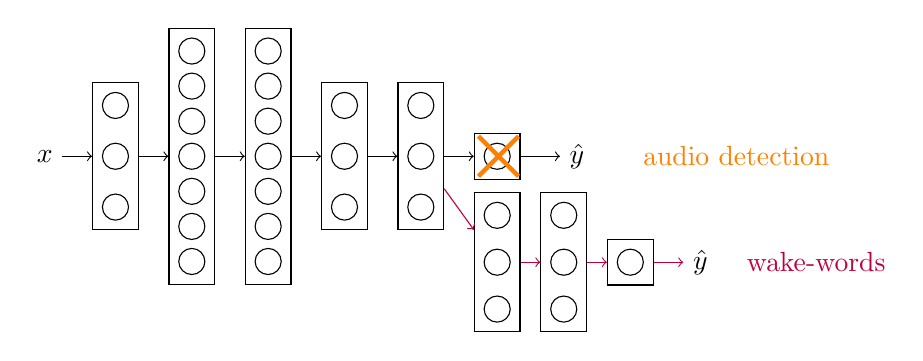
\begin{tikzpicture}[darkstyle/.style={circle,draw,fill=gray!40,minimum size=20}]
  \node (x) at (0, 0) {$x$};
  \node[draw, circle, right = 0.5cm of x] (l10) {};
  \node[draw, circle, above = .3cm of l10] (l11) {};
  \node[draw, circle, below = .3cm of l10] (l12) {};
  \node[draw, fit = (l10) (l11) (l12)] (layer1) {};
  \draw[->] (x) to (layer1);
  \node[draw, circle, right = 0.5cm of layer1] (l20) {};
  \node[draw, circle, above = .1cm of l20] (l21) {};
  \node[draw, circle, above = .1cm of l21] (l22) {};
  \node[draw, circle, above = .1cm of l22] (l23) {};
  \node[draw, circle, below = .1cm of l20] (l24) {};
  \node[draw, circle, below = .1cm of l24] (l25) {};
  \node[draw, circle, below = .1cm of l25] (l26) {};
  \node[draw, fit = (l23) (l26)] (layer2) {};
  \draw[->] (layer1) to (layer2);  
  \node[draw, circle, right = 0.5cm of layer2] (l30) {};
  \node[draw, circle, above = .1cm of l30] (l31) {};
  \node[draw, circle, above = .1cm of l31] (l32) {};
  \node[draw, circle, above = .1cm of l32] (l33) {};
  \node[draw, circle, below = .1cm of l30] (l34) {};
  \node[draw, circle, below = .1cm of l34] (l35) {};
  \node[draw, circle, below = .1cm of l35] (l36) {};
  \node[draw, fit = (l33) (l36)] (layer3) {};
  \draw[->] (layer2) to (layer3);  
  \node[draw, circle, right = 0.5cm of layer3] (l40) {};
  \node[draw, circle, above = .3cm of l40] (l41) {};
  \node[draw, circle, below = .3cm of l40] (l42) {};
  \node[draw, fit = (l40) (l41) (l42)] (layer4) {};
  \draw[->] (layer3) to (layer4);
  \node[draw, circle, right = 0.5cm of layer4] (l50) {};
  \node[draw, circle, above = .3cm of l50] (l51) {};
  \node[draw, circle, below = .3cm of l50] (l52) {};
  \node[draw, fit = (l50) (l51) (l52)] (layer5) {};
  \draw[->] (layer4) to (layer5);
  \node[draw, circle, right = 0.5cm of layer5] (fnode) {};
  \node[draw, fit = (fnode)] (fnodebox) {};
  \draw[->] (layer5) to (fnodebox);
  \node[right = 0.5cm of fnodebox] (yhat) {$\hat y$};
  \draw[->] (fnodebox) to (yhat);
  \node[right = 0.5cm of yhat] (imagerecog) {\color{orange} \textrm{audio detection}};
  \node[draw, ultra thick, orange, right = 0.435cm of layer5, cross out, scale = 1.75] {};
  \node[below = 1cm of fnode, draw, circle] (newnode) {};
  \node[above = 0.25cm of newnode, draw, circle] (newnodep1) {};
  \node[below = 0.25cm of newnode, draw, circle] (newnodem1) {};
  \node[draw, fit = (newnodem1) (newnodep1)] (newnodebox) {};
  \draw[->, purple] (layer5) to (newnodebox);
  \node[right = 0.5cm of newnode, draw, circle] (lastlayercentered) {};
  \node[below = 0.25cm of lastlayercentered, draw, circle] (lastlayerminus) {};
  \node[above = 0.25cm of lastlayercentered, draw, circle] (lastlayerplus) {};
  \node[draw, fit = (lastlayerminus) (lastlayerplus)] (lastlayer) {};
  \node[right = 0.5cm of lastlayercentered, draw, circle] (lastnode) {};
  \node[draw, fit = (lastnode)] (penultimate) {};
  \node[right = 0.5cm of lastnode] (newyhat) {$\hat y$};
  \draw[->, purple] (newnodebox) to (lastlayer);
  \draw[->, purple] (lastlayer) to (penultimate);
  \draw[->, purple] (penultimate) to (newyhat);
  \node[right = 0.25cm of newyhat] {\color{purple} wake-words};
\end{tikzpicture}
\caption{\footnotesize In another example, we demonstrate transfer learning with wake-words. Here, we not only modify the last output layer to 
output a prediction in wake-word space, but we also incorporate several additional intermediary layers. Depending on how much
wake-words data we have available to train on, we can choose to either only train the weights of the newly incorporated/modified layers \emph{or} we can choose to re-train the entire network.}
\end{figure}

\paragraph{When does transfer learning make sense?}
It only makes sense to apply transfer learning when the inputs for both tasks are the same. E.g. in our examples above, the inputs were images in one example and audio clips in another. Further, transfer learning makes sense when we have a lot of data for the problem you're transfer learning from, and relatively less data for the problem you're transferring to. Let's reconsider our examples. In the context of image recognition, it's not uncommon to end up with a million examples for a particular task, which is quite a lot of data to learn low-level and useful features in earlier layers of our network. On the other hand, we may only have a few hundred examples for our radiology diagnosis
problem. A lot of the knowledge that we learned from image recognition can be transferred and can greatly help radiology
diagnosis even without a lot of radiology data. In the context of our speech recognition example, 
we might have 10,000 hours of data which is quite a lot, but for trigger words perhaps we only have one hour of data. In this case,
a lot of what the network learns about what human voices sound like, what the components of speech are, and so on,
can be really helpful in building a good wake-words detector. It \emph{doesn't} make sense to use transfer learning when we have little data to pre-train our network on and relatively more data to fine-tune the network on; in these cases we need to remember what
our core task is and recognize which training examples are the most informative.

\subsubsection{Multi-task Learning} In transfer learning, we have a sequential process: we start learning how to perform task A
and then transfer that knowledge to task B. In multi-task learning, we start simultaneously and try to have one neural network do several things at the same time (with the hope that each of these tasks helps in solving the other tasks).
\begin{table}[h]
  \centering
  \begin{tabular}{l | c}     & $y^{(i)}$ \\
    \hline
    Pedestrians & 0 \\
    Cars & 1 \\
    Stop-signs & 1 \\
    Traffic-lights & 0     \end{tabular}
\caption{\footnotesize In multi-task learning, our input is an image $x^{(i)}$ and our output
  $y^{(i)}$ may have one entry for each task we are interested in. Suppose you're building a self-driving car, which needs to be able to detect several types of objects like pedestrians, other cars, stop signs, traffic lights,
and maybe even other things.
 If we have an image of a car at a stop-sign, then we would
  expect the following output vector to be associated with the example.} 
\end{table} 

\begin{figure}[h]
\centering
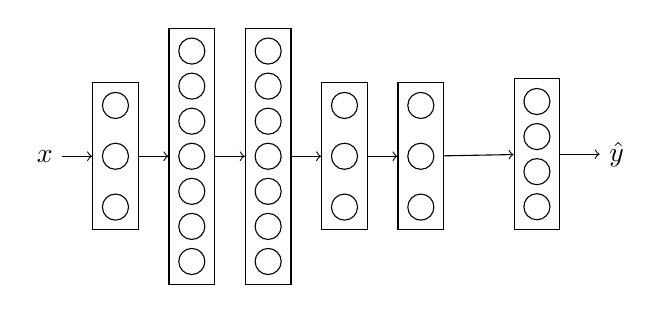
\begin{tikzpicture}[darkstyle/.style={circle,draw,fill=gray!40,minimum size=20}]
  \node (x) at (0, 0) {$x$};
  \node[draw, circle, right = 0.5cm of x] (l10) {};
  \node[draw, circle, above = .3cm of l10] (l11) {};
  \node[draw, circle, below = .3cm of l10] (l12) {};
  \node[draw, fit = (l10) (l11) (l12)] (layer1) {};
  \draw[->] (x) to (layer1);
  \node[draw, circle, right = 0.5cm of layer1] (l20) {};
  \node[draw, circle, above = .1cm of l20] (l21) {};
  \node[draw, circle, above = .1cm of l21] (l22) {};
  \node[draw, circle, above = .1cm of l22] (l23) {};
  \node[draw, circle, below = .1cm of l20] (l24) {};
  \node[draw, circle, below = .1cm of l24] (l25) {};
  \node[draw, circle, below = .1cm of l25] (l26) {};
  \node[draw, fit = (l23) (l26)] (layer2) {};
  \draw[->] (layer1) to (layer2);  
  \node[draw, circle, right = 0.5cm of layer2] (l30) {};
  \node[draw, circle, above = .1cm of l30] (l31) {};
  \node[draw, circle, above = .1cm of l31] (l32) {};
  \node[draw, circle, above = .1cm of l32] (l33) {};
  \node[draw, circle, below = .1cm of l30] (l34) {};
  \node[draw, circle, below = .1cm of l34] (l35) {};
  \node[draw, circle, below = .1cm of l35] (l36) {};
  \node[draw, fit = (l33) (l36)] (layer3) {};
  \draw[->] (layer2) to (layer3);  
  \node[draw, circle, right = 0.5cm of layer3] (l40) {};
  \node[draw, circle, above = .3cm of l40] (l41) {};
  \node[draw, circle, below = .3cm of l40] (l42) {};
  \node[draw, fit = (l40) (l41) (l42)] (layer4) {};
  \draw[->] (layer3) to (layer4);
  \node[draw, circle, right = 0.5cm of layer4] (l50) {};
  \node[draw, circle, above = .3cm of l50] (l51) {};
  \node[draw, circle, below = .3cm of l50] (l52) {};
  \node[draw, fit = (l50) (l51) (l52)] (layer5) {};
  \draw[->] (layer4) to (layer5);
  \node[draw, circle] (fnode) at (6.25, 0.25) {};
  \node[draw, circle, above = 0.1cm of fnode] (fnodep) {};
  \node[draw, circle, below = 0.1cm of fnode] (fnodeb) {};
  \node[draw, circle, below = 0.1cm of fnodeb] (fnodebb) {};
  \node[draw, fit = (fnodebb) (fnodep)] (fnodebox) {};
  \draw[->] (layer5) to (fnodebox);
  \node[right = 0.5cm of fnodebox] (yhat) {$\hat y$};
  \draw[->] (fnodebox) to (yhat);
\end{tikzpicture}
\caption{\footnotesize Note that here our last layer has as many nodes as there are tasks we trying to solve, and correspondingly
the dimension of $\hat y$ will be the same as well.}
\end{figure}

\paragraph{Loss for a multi-task problem} Let $|y|$ denote the dimension of our output vector. We could define a cost function to be
\begin{equation*}   \sum_{i=1}^m \sum_{j=1}^{|y|} \mathcal L(\hat y_j^{(i)}, y_j^{(i)}) \end{equation*}
where $\mathcal L(\cdot, \cdot)$ is our usual Logistic loss function for a binary prediction problem. What's the difference between this and using softmax regression? In softmax regression, we assign a single label to each (training) example, whereas in multi-task
learning each example can have multiple labels. Note that we could have trained $|y|$ separate neural networks to each solve one task. But, if some of the earlier features in the neural network can be shared between different tasks, then you might find that training a single neural network to solve multiple tasks results in better performance.

\paragraph{Multi-task learning works even if inputs aren't ``fully'' labeled} Suppose we are still in the setting of self-driving cars and we have an image of a car at a stop-sign, but that our human-labeler didn't bother to mark the image as having both
a car and a stop-sign (just one of them). Maybe we're in the setting where some of our examples \emph{are} fully labeled, but others
are not. In this setting, it's still valid to perform multi-task learning. In particular, we modify our loss-function to only sum over the indices of $j$ which correspond to having been labeled. I.e.
\begin{equation*}   
  \sum_{i=1}^m \sum_{j=1}^{|y|} \mathcal L(\hat y_j^{(i)}, y_j^{(i)}) \mathbbm 1_{\{\textrm{Category } j \textrm{ was labeled on example } i\}} 
\end{equation*}

\paragraph{When does multi-task learning make sense?} It makes sense in general when three things are true.
\begin{enumerate}   \item  If the set of tasks could benefit from having shared low-level features. E.g. in the context of autonomous driving, being able to recognize traffic lights, cars, and pedestrians may help us learn features that also distinguish stop signs.
  \item If the amount of data available for each task is similar. As a soft rule, we expect a single task to benefit from multi-task
    learning if the amount of data available from all other tasks is at least as large as the amount of data we have at hand
    for one task; the reasons why are similar to when transfer learning does and doesn't work.
  \item Can train a big enough network to do well on all tasks. From researcher Rich Carona, the only times 
    that multi-task learning hurts performance compared to training separate neural networks is if your 
    neural network isn't big enough. If you can train a large enough network, multi-task learning shouldn't hurt performance. \end{enumerate}

\subsection{End-to-End Deep Learning} One of the most exciting recent developments in deep learning has been the rise
of end-to-end deep learning. What does this mean? Briefly, it means learning systems that require multiple stages of processing
and replacing it by a single neural network. Consider an example of speech recognition, where the goal is to take an input $x$
such as an audio clip and map it to a transcript $y$. Traditional speech recognition methods require many stages of processing,
e.g. \href{https://en.wikipedia.org/wiki/Mel-frequency_cepstrum}{MFCC} which is an algorithm for extracting hand designed features
of audio. Having extracted these low level features, you might apply a machine learning algorithm to find the \href{https://en.wikipedia.org/wiki/Phoneme}{phonemes} in the audio clip, the basic units of sound; e.g. the word ``cat'' consists of three sounds: ``cu'', ``ah'', and ``tu''. After phonemes are extracted, we can string them together to form words, and finally stringing together words
we get a transcript.

\begin{figure}[h]   \centering
  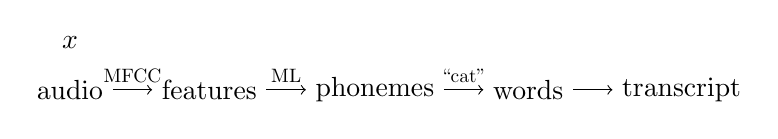
\begin{tikzpicture}     \node (x) at (0.15,0) {$x$};
    \node[below=0.15cm of x] (a) {audio};
    \node[right=0.5cm of a] (f) {features};
    \node[right=0.5cm of f] (p) {phonemes};
    \node[right=0.5cm of p] (w) {words};
    \node[right=0.5cm of w] (t) {transcript};
    \draw[->] (a) -- (f) node[midway,above,scale=0.7] {\textrm{MFCC}};
    \draw[->] (f) -- (p) node[midway,above,scale=0.7] {\textrm{ML}};     \draw[->] (p) -- (w) node[midway,above,scale=0.7] {``cat''}; 
    \draw[->] (w) -- (t) node[midway,above,scale=0.7] {}; 
  \end{tikzpicture}
  \caption{\footnotesize A classical pipeline for processing audio into transcripts. Such a sequential system of algorithms is no longer necessary with end-to-end deep learning: a neural network can accept as input an audio clip and return as output a transcript. Andrew admits that end-to-end deep learning systems have made obsolete many sub-fields which used to exist and which were predicated on delicate feature engineering for their particular sub-task.} \end{figure}

One downside of end-to-end learning is that you might need a lot of data before it starts to work well; for smaller sized data sets,
the hand-engineered approaches can be quite competitive. If you have a medium amount of data, there are intermediary approaches
where perhaps in our example you input the audio and bypass the features and just learn to output phonemes, and then there would be some other steps involved as well: this would be a step towards end-to-end learning.

Let's consider an interesting example of face recognition at turnstiles in public transit systems: if the system recognizes the face
it shall allow the person to pass without needing to scan an RFID card. The input here is an image which contains a person approaching the turnstile, and we could try to learn a mapping from this raw image $X$ to the identity of the person $Y$, but this turns out to \emph{not} be the best approach: the person can approach the turnstile from different directions and they can be at varying distances from the camera whereby their face appears much larger. The best approach to date is a multi-step approach where first one piece of software is run to detect \emph{where} the person's face is within the image, and as a secondary step the image is cropped 
and centered to a new neural network that tries to learn the person's \emph{identity}. 
Researchers have found that breaking the problem into two stages has resulted in the best performance.\footnote{The way the second neural network works is that it takes as input two images, and it returns whether the images contain the same person or not. In our application, the background database would consist of facial images for all employees on file: the algorithm would then scan through
all the background images and see whether the input image contains a face that matches a face contained in the database.}
Why does the two step approach work better? There are two reasons.
\begin{itemize}   
  \item Each subproblem is much simpler.
  \item Each sub-task is amenable to producing a lot of data. 
\end{itemize}
In particular, there's a lot of data one could obtain that maps input images $X$ to bounded boxes $y$ describing where a persons face in the image lie. Separately, there's a lot of data for looking at two images and determining whether its the same person. But in contrast, if you try to learn everything at the same time, there is much less data of the form $(X,Y)$ where $X$ is an input image from a turnstile, and $Y$ is the identity of the person. One example where end-to-end deep learning does work well is in machine translation, since for any arbitrary pair of countries we have a lot of mappings or translations.

\paragraph{Whether to use End-to-End deep learning}

\begin{itemize}   \item Pros
    \begin{itemize}       \item End-to-end learning lets the data speak: no matter what $(X,Y)$ mapping truly exists,
        with enough data and a big enough network, we should be able to learn the function mapping
        from $X$ to $Y$. Further, a pure machine learning approach allows the neural network to capture statistics
        of the data rather than being forced to reflect human preconceptions.\footnote{Consider an example of speech recognition. 
        Andrew believes that phonemes are an artifact created by linguists that are reasonable to the description of language. 
        However, it's not obvious that you want to force your learning algorithm to think in phonemes.}
    \item There is less hand designing of components needed, which means less time spent hand-engineering features or
      designing intermediate representations.     \end{itemize}
  \item Cons
    \begin{itemize}     \item May require a large amount of data to learn an end-to-end mapping from raw $X$ to $Y$. 
      We've seen previously that it can be easier to acquire
      data for sub-tasks, e.g. first finding a face within an image then determining if the face matches
      one in a database.
    \item It excludes potentially useful hand-designed components. If you don't have a lot of data, then
      your learning algorithm won't yield that much insight, and so hand designing a component can
      be a way to inject manual knowledge into an algorithm (which is not always a bad thing).     \end{itemize} \end{itemize} 

A learning algorithm has two main sources of knowledge: (i) the data, and (ii) whatever you hand design. If you have tons of data,
it's less important to hand-design things, but without much data hand-design becomes more important. They key question to answer when determining whether to use an end-to-end approach is: do I have sufficient data to learn the function of the complexity needed
to map $X$ to $Y$.

As an example of the boundary between end-to-end learning, consider self-driving cars. If we don't take an end-to-end approach,
we could take as input an image of what's in front of the car (perhaps obtained through picture, radar, lidar, or other sensor readings) and (i) try to figure out what objects are in the image, (ii) how to navigate the car safely around the pedestrians and cars spotted, and (iii) execute the plan with appropriate steering as well as acceleration and braking. Step two is usually not performed by a neural network, but instead by a piece of software called \href{https://en.wikipedia.org/wiki/Motion_planning}{Motion Planning}. As of this writing, Andrew believes that end-to-end learning is less effective than more sophisticated hand-engineered approaches.

\section{Convolutional Neural Networks} Computer vision is an area with a rapidly growing research body. E.g.,
computer vision can
\begin{itemize} 
\item Help self-driving cars figure out where the other cars and pedestrians are in order to avoid them.
\item Allow an individual to unlock a phone or door with just their face.
\item Show you the most attractive, beautiful, or relevant pictures. \end{itemize}

Deep learning is even helping new types of art to be created (see \href{https://en.wikipedia.org/wiki/Neural_Style_Transfer}{Neural Style Transfer}). Rapid advances in computer vision enable new applications
that were impossible just a few years ago. Lastly, computer vision researchers are quite cunning and there is a lot of
inspiration to be drawn from this sub-field. Let's start by reviewing some examples of computer vision.
\begin{itemize}   \item Image classification: you're given a 64x64 pixel image and asked to output a single bit describing 
    whether it contains a cat.
  \item Object Detection: you're given an image and you must determine what objects are in the picture but also draw bounding boxes around them. \end{itemize}

\paragraph{Size of input data $\leadsto$ Convolution Operation} 
If we work with a 64x64 image, and since we have three color channels RGB, each image or input is
$64^2 \cdot 3 = 12,288$ dimensional. But, this was a tiny image, what if we had a $1,000 x 1,000$ pixel image (one megapixel)? Then
each input has $1e3^2 \cdot 3 = 3e6 = 3,000,000$ or three million dimensions. What if we have 1,000 hidden units in our first layer?
Then $W^{[1]}$ will be of size $1k x 3M$ which is 3 billion parameters; with that many parameters it's difficult to get enough
data to prevent overfitting, and further the computational (and memory) requirements to train a neural network with three billion
parameters is not yet feasible. All of this is to say that if you want to use large images, you need to better implement the
convolution operation.

\subsection{Edge detection} Earlier layers of a neural network might detect edges, later layers may detect parts
of objects, and later layers still may detect complete objects such as a person's face. In this section, we'll focus on edge 
detection. 
\subsubsection{Filters and kernels}
Suppose that we have a simple $6 \times 6$ matrix that represents a grey-scale image (we don't need the three RGB channels).
\begin{equation*}   \begin{bmatrix}     3 & 0 & 1 & 2 & 7 & 4 \\
    1 & 5 & 8 & 9 & 3 & 1 \\     2 & 7 & 2 & 5 & 1 & 3 \\     
    0 & 1 & 3 & 1 & 7 & 8 \\     
    4 & 2 & 1 & 6 & 2 & 8 \\     
    2 & 4 & 5 & 2 & 3 & 9 \\ 
  \end{bmatrix} \end{equation*}

How can we extract vertical edges? We start by constructing a $3 \times 3$ \emph{filter} matrix (also sometimes referred to as a kernel).
\begin{equation*}   \begin{bmatrix}     1 & 0 & -1 \\     1 & 0 & -1 \\
    1 & 0 & -1 \\
  \end{bmatrix} \end{equation*}

Now, what we'll do is take our original image and \emph{convolve} it with the filter; the symbol used to denote convolution is $*$,
which is distinguished from multiplication by context. The output of convolving our $6 \times 6$ image is a $4 \times 4$ matrix. Let's consider how to apply the convolution to our input image to yield the first element in the output; to do this we'll examine the first few rows and columns of our input:

\begin{equation*}   
  \begin{bmatrix}     
    3 & 0 & 1 \\
    1 & 5 & 8 \\     
    2 & 7 & 2 \\     
  \end{bmatrix} 
  *
  \begin{bmatrix}     
    1 & 0 & -1 \\     
    1 & 0 & -1 \\
    1 & 0 & -1 \\
  \end{bmatrix}
  = 3\cdot 1 + 1 \cdot 1 + 2\cdot 1 + 0\cdot 0 + 5 \cdot 0 + 7 \cdot 0 + 1 \cdot -1 + 8 \cdot -1 + 2 \cdot -1 = -5.
\end{equation*}
Notice that this is a simple element-wise product followed by a summation. To continue the process, we move the filter
over by one column and repeat the same process (element-wise multiplication followed by summation) 
to get the output for the second item in the first row. Continuing on, we get

\begin{equation*}   
  \begin{bmatrix}     
    3 & 0 & 1 & 2 & 7 & 4 \\
    1 & 5 & 8 & 9 & 3 & 1 \\     
    2 & 7 & 2 & 5 & 1 & 3 \\     
    0 & 1 & 3 & 1 & 7 & 8 \\     
    4 & 2 & 1 & 6 & 2 & 8 \\     
    2 & 4 & 5 & 2 & 3 & 9 \\ 
  \end{bmatrix} 
  *
  \begin{bmatrix}     
    1 & 0 & -1 \\     
    1 & 0 & -1 \\
    1 & 0 & -1 \\
  \end{bmatrix}
  = \begin{bmatrix}     -5 & -4 & 0 & 8 \\
    -10 & -2 & 2 & 3 \\
    0 & -2 & -4 & -7 \\
    -3 & -2 & -3 & -16   \end{bmatrix}.
\end{equation*}

This turns out to detect (vertical) edges. Why? Let's first consider a simpified example
\begin{equation*}   \begin{bmatrix}
 10 & 10 & 10 & 0 & 0 & 0 \\
 10 & 10 & 10 & 0 & 0 & 0 \\
 10 & 10 & 10 & 0 & 0 & 0 \\
 10 & 10 & 10 & 0 & 0 & 0 \\
 10 & 10 & 10 & 0 & 0 & 0 \\
 10 & 10 & 10 & 0 & 0 & 0
  \end{bmatrix} \end{equation*}
Mathematically,
\begin{equation*}   \begin{bmatrix}
 10 & 10 & 10 & 0 & 0 & 0 \\
 10 & 10 & 10 & 0 & 0 & 0 \\
 10 & 10 & 10 & 0 & 0 & 0 \\
 10 & 10 & 10 & 0 & 0 & 0 \\
 10 & 10 & 10 & 0 & 0 & 0 \\
 10 & 10 & 10 & 0 & 0 & 0
  \end{bmatrix} 
  * 
  \begin{bmatrix}     
    1 & 0 & -1 \\     
    1 & 0 & -1 \\
    1 & 0 & -1 \\
  \end{bmatrix}
  =
  \begin{bmatrix}     0 & 30 & 30 & 0 \\
    0 & 30 & 30 & 0 \\
    0 & 30 & 30 & 0 \\
    0 & 30 & 30 & 0 \\
  \end{bmatrix} \end{equation*}
If we were to visualize this image, it might look as follows:

\begin{figure}[h]   
  \centering
  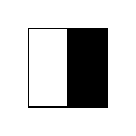
\begin{tikzpicture}[scale=0.5]     
    \draw[fill = white, black] (1,0) rectangle (2, 2);     
    \draw[fill = white] (0,0) rectangle (1, 2); 
  \end{tikzpicture} 
\end{figure} 
The larger values yield brighter pixel intensive values. In this image, there is very clearly a vertical edge right down the middle.
We can visualize our filter or kernel matrix as well.
\begin{figure}[h]
  \centering
  
\begin{tikzpicture}[scale=0.5]     \draw[fill = white] (0,0) rectangle (1, 2); 
    \draw[fill = white, black] (1,0) rectangle (2, 2);     
    \node at (3, 1) {*};
    \draw[fill = white] (4,0) rectangle (4.6666, 2); 
    \draw[fill = gray]  (4.6666,0) rectangle (5.3333, 2);
    \draw[fill = black] (5.3333,0) rectangle (6, 2);     
    \node at (7, 1) {=};
    \draw[fill = black] (8,0) rectangle (8.6666, 2); 
    \draw[fill = white]  (8.6666,0) rectangle (9.3333, 2);
    \draw[fill = black] (9.3333,0) rectangle (10, 2);     
  \end{tikzpicture} \end{figure}

Two remarks: (i) since our image is small ($64 \times 64$), the vertical edge detected appears ``quite wide'', but this is simply
an artifact of having a small-resolution image, and (ii) the enhanced pixel intensity in the middle of the output is a way of
saying that there exists a strong vertical edge in this part of the original image.

\subsubsection{Positive and negative edges} 
We define a positive edge as one where the light goes from light to dark, versus a negative edge
which goes from a dark to a light transition. We will learn about other edge detectors, and also have a chance to understand
how an algorithm can learn to construct a filter (rather than creating one by hand).

Note that the filter we used above does take into account positive versus negative edges. If our input image was flipped
then the signs of the entries would inform us whether the edge is positive or negative.
\begin{equation*}   \begin{bmatrix}
 0 & 0 & 0 & 10 & 10 & 10 \\
 0 & 0 & 0 & 10 & 10 & 10 \\
 0 & 0 & 0 & 10 & 10 & 10 \\
 0 & 0 & 0 & 10 & 10 & 10 \\
 0 & 0 & 0 & 10 & 10 & 10 \\
 0 & 0 & 0 & 10 & 10 & 10
  \end{bmatrix} 
  * 
  \begin{bmatrix}     
    1 & 0 & -1 \\     
    1 & 0 & -1 \\
    1 & 0 & -1 \\
  \end{bmatrix}
  =
  \begin{bmatrix}     0 & -30 & -30 & 0 \\
    0 & -30 & -30 & 0 \\
    0 & -30 & -30 & 0 \\
    0 & -30 & -30 & 0 \\
  \end{bmatrix} 
\end{equation*}

As a picture, this might look like:
\begin{figure}[h]
  \centering
  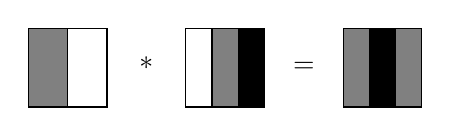
\begin{tikzpicture}[scale=0.5]
    \draw[fill = gray] (0,0) rectangle (1, 2); 
    \draw[fill = white] (1,0) rectangle (2, 2);     
    \node at (3, 1) {*};
    \draw[fill = white] (4,0) rectangle (4.6666, 2); 
    \draw[fill = gray]  (4.6666,0) rectangle (5.3333, 2);
    \draw[fill = black] (5.3333,0) rectangle (6, 2);     
    \node at (7, 1) {=};
    \draw[fill = gray] (8,0) rectangle (8.6666, 2); 
    \draw[fill = black]  (8.6666,0) rectangle (9.3333, 2);
    \draw[fill = gray] (9.3333,0) rectangle (10, 2);     
\end{tikzpicture} 
\end{figure}

Since the shade of transitions is now reversed, so are the signs on the values
in our matrix. If you don't care whether the edge is positive or negative,
it's reasonable to take absolute values of the output.

\subsubsection{Horizontal Edges} It may not be surprising to learn that the filter
matrix used to detect horizontal edges is simply a transpose of the filter matrix
used to detect vertical edges. I.e.
\begin{equation*} \begin{bmatrix}   1 & 1 & 1 \\ 0 & 0 & 0 \\ -1 & -1 & -1 \end{bmatrix}   \end{equation*}
Let's consider a more interesting example. The matrix
\begin{equation}   \begin{bmatrix}     10 & 10 & 10 & 0 & 0 & 0 \\
    10 & 10 & 10 & 0 & 0 & 0 \\
    10 & 10 & 10 & 0 & 0 & 0 \\
    0 & 0 & 0 & 10 & 10 & 10 \\
    0 & 0 & 0 & 10 & 10 & 10 \\
    0 & 0 & 0 & 10 & 10 & 10 \\   \end{bmatrix} \end{equation}
As applied to our filter:
\begin{equation*}   \begin{bmatrix}     
    10 & 10 & 10 & 0 & 0 & 0 \\
    10 & 10 & 10 & 0 & 0 & 0 \\
    10 & 10 & 10 & 0 & 0 & 0 \\
    0 & 0 & 0 & 10 & 10 & 10 \\
    0 & 0 & 0 & 10 & 10 & 10 \\
    0 & 0 & 0 & 10 & 10 & 10 \\       \end{bmatrix}
  *
  \begin{bmatrix}   1 & 1 & 1 \\ 0 & 0 & 0 \\ -1 & -1 & -1 \end{bmatrix}.
  =
  \begin{bmatrix}     0 & 0 & 0 & 0 \\
    30 & 10 & -10 & 30 \\
    30 & 10 & -10 & 30 \\
    0 & 0 & 0 & 0   \end{bmatrix} \end{equation*}
Graphically, our input image is ``lit-up'' in the upper left and lower right hand corners.
\begin{figure}[h]   \centering
  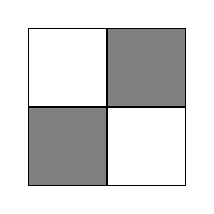
\begin{tikzpicture}     \draw[fill=gray] (0,0) rectangle (1,1);
    \draw (0,1) rectangle (1,2);      \draw[fill=gray] (1,1) rectangle (2,2);
    \draw (1,0) rectangle (2,1);
  \end{tikzpicture} \end{figure}
Andrew comments that the fact we see intermediate values in the middle columns is an artifact of using a low-resolution
input image. In the cases where the filter outputs $\pm 10$ in our example above, this reflects the fact that the filter
captures positive edges on one side and negative edges on the other, and so blending these together gives an intermediary value.

There is another filter matrix we could use, called a Sobel filter. It's shaped like
\begin{equation*}   
  \begin{bmatrix}     1 & 2 & 1 \\ 0 & 0 & 0 \\ -1 & -2 & -1     \end{bmatrix}
\end{equation*}

The advantage of this filter is that it places more weight on the central pixel, and this can make
the filter a bit more robust. Computer vision researchers will try other weights as well. E.g. the Scharr filter,

\begin{equation*}   
  \begin{bmatrix}     3 & 10 & 3 \\ 0 & 0 & 0 \\ -3 & -10 & -3     \end{bmatrix}
\end{equation*}
This filter has other properties. What we've shown above is just for \emph{vertical} edge detection,
but we can also transpose each of these filters to get a \emph{horizontal} edge detector.
With the rise of deep learning, perhaps we don't need to pick these numbers by hand: we can instead treat these
as parameters and have the neural network learn weights through back propagation, where the goal is to learn nine
parameters so that when you take the image and convolve it with the filter, we yield a ``good'' edge detector.
If the network wants, it can learn the same values as what are in a Sobel or Scharr filter, but its more likely they
will learn something else that is even more effective at detecting edges. Further, perhaps we can learn filters which
detect edges at arbitrary angles (e.g. an edge at 45 degrees). Underlying all these computations is the convolution,
which allows back propagation to learn whatever filter it wants.

\subsection{Padding} One modification we can make to the basic convolutional operation is padding. In general, if we have
an $n \times n$ matrix with an $f \times f$ size filter, the output will be of size $(n-f+1) \times (n-f+1)$. There are two downsides
here:
\begin{enumerate} \item Every time we apply a convolution operator, our image shrinks. Perhaps we don't want our image to shrink each time
  we detect edges or other features; if we have many layers in our network then the latter layers take as input
  a shrunken image which could end up being a $1 \times 1$ pixel in the end.
\item If we examine corner pixels, we notice that the filter only \emph{touches} the pixel once, whereas for a pixel
in the middle of the image there are many $f \times f$ regions that overlap with the pixel. And so, it's as if pixels on
the corners of the image are used much less in the output; it's as though we're throwing away a lot of information
for these corner pixels. \end{enumerate}

\begin{figure}[h]   \centering
  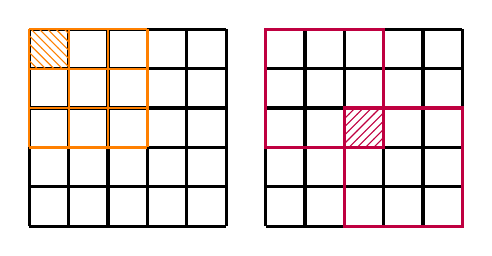
\begin{tikzpicture}[scale=0.5]     \draw[step=1.0, very thick] (0,0) grid (5,5);
    \filldraw[pattern=north west lines,pattern color=orange] (0,4) rectangle(1,5);
    \draw[step=1.0, thick, orange] (0,2) grid (3,5);
    \draw[step=1.0, very thick] (6,0) grid (11, 5);
    \filldraw[pattern=north east lines, pattern color = purple] (8,2) rectangle (9,3);
    \draw[step=1.0, very thick, purple] (8,3) rectangle (11,0);
    \draw[step=1.0, very thick, purple] (6,5) rectangle (9,2);
  \end{tikzpicture}
  \caption{\footnotesize On the left, we visualize how the upper-left pixel can only be touched once by a filter. On the right,
    we highlight a central cell and visualize how it can be touched by more than one filter.} \end{figure}

To fix both of these problems, we can \emph{pad} our input image.
\begin{figure}   \centering
  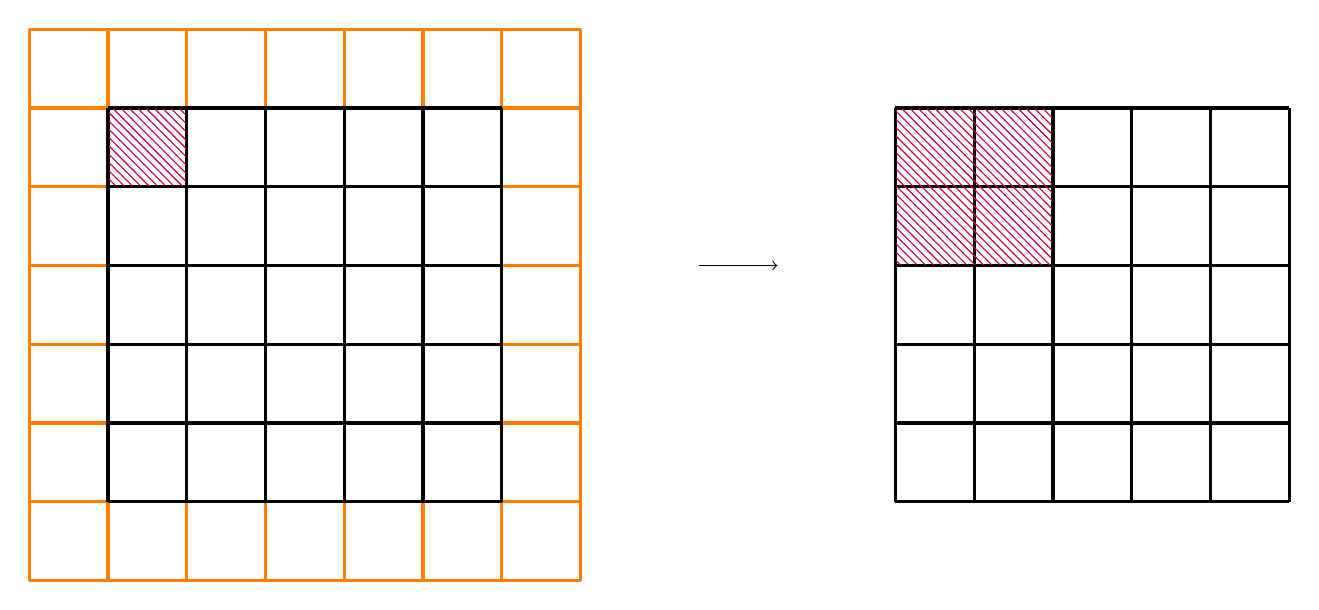
\begin{tikzpicture}     \draw[step=1.0, very thick, orange] (-1,-1) grid (6,6);
    \draw[step=1.0, very thick]         (0, 0) grid (5,5);
    \filldraw[pattern=north west lines,pattern color=purple] (0,4) rectangle(1,5);
    \draw[->] (7.5, 3) -- (8.5, 3);
    \draw[step=1.0, very thick]         (10, 0) grid (15,5);
    \filldraw[pattern = north west lines, pattern color = purple] (10,5) rectangle (12,3);   \end{tikzpicture}
  \caption{\footnotesize If we pad our input image with two additional rows and two additional columns (depicted on the left), 
    we preserve the size of the image
    in the output. Further, corner cells are able to \emph{influence} the more than just one value in the output image 
    (depicted on the right).} \end{figure}

\subsubsection{Dimension of padded images}
Now, if we take our \emph{padded} image and apply a convolution operation, we manage
to preserve the size of the input image. I.e. the convolution outputs an image of the same size
as the input. By convention, we pad with zeros. In general, if we pad with $p$ additional cells
on each side of the image, then our input image has dimension $(n+2p) \times (n+2p)$, and if we apply a convolution
operation we end up with a $(n+2p-f+1) \times (n+2p-f+1)$ output image. 

\paragraph{Preserving input size with padding}
If we want
our output image to be $n \times n$, then we can set up a simple equation and solve for $p$:
\begin{equation*}   n + 2p - f + 1 = n \implies p = \frac{f-1}{2}, \end{equation*}
which means that if $f$ is odd this means we have a symmetric padding around the image.\footnote{Note that if $f$ is odd, it has a central pixel. This can sometimes be handy to reference.}

\subsection{Strided Convolutions}

\paragraph{Types of Convolution} There are two common choices for padding,
called Valid convolutions and Same convolutions. A valid convolution
uses no padding. The other choice is Same convolutions, in which the output
image is the same size as the input image.

\begin{figure}[h]   \centering
  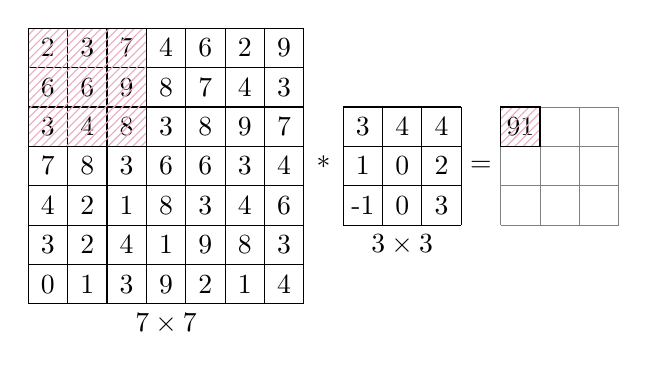
\begin{tikzpicture}[scale=0.5]       \draw[step=1cm] (0, 0) grid (7, 7);
      % Starting from bottom row, working left to right.
      \node at (0.5, 0.5) {0};
      \node at (1.5, 0.5) {1};
      \node at (2.5, 0.5) {3};
      \node at (3.5, 0.5) {9};
      \node at (4.5, 0.5) {2};
      \node at (5.5, 0.5) {1};
      \node at (6.5, 0.5) {4};
      % second row from bottom.
      \node at (0.5, 1.5) {3};
      \node at (1.5, 1.5) {2};
      \node at (2.5, 1.5) {4};
      \node at (3.5, 1.5) {1};
      \node at (4.5, 1.5) {9};
      \node at (5.5, 1.5) {8};
      \node at (6.5, 1.5) {3};
      % Third from bottom.
      \node at (0.5, 2.5) {4};
      \node at (1.5, 2.5) {2};
      \node at (2.5, 2.5) {1};
      \node at (3.5, 2.5) {8};
      \node at (4.5, 2.5) {3};
      \node at (5.5, 2.5) {4};
      \node at (6.5, 2.5) {6};
      % Fourth from bottom.
      \node at (0.5, 3.5) {7};
      \node at (1.5, 3.5) {8};
      \node at (2.5, 3.5) {3};
      \node at (3.5, 3.5) {6};
      \node at (4.5, 3.5) {6};
      \node at (5.5, 3.5) {3};
      \node at (6.5, 3.5) {4};
      % Fifth from bottom
      \node at (0.5, 4.5) {3};
      \node at (1.5, 4.5) {4};
      \node at (2.5, 4.5) {8};
      \node at (3.5, 4.5) {3};
      \node at (4.5, 4.5) {8};
      \node at (5.5, 4.5) {9};
      \node at (6.5, 4.5) {7};
      % Second from top.
      \node at (0.5, 5.5) {6};
      \node at (1.5, 5.5) {6};
      \node at (2.5, 5.5) {9};
      \node at (3.5, 5.5) {8};
      \node at (4.5, 5.5) {7};
      \node at (5.5, 5.5) {4};
      \node at (6.5, 5.5) {3};
      % Top row.
      \node at (0.5, 6.5) {2};
      \node at (1.5, 6.5) {3};
      \node at (2.5, 6.5) {7};
      \node at (3.5, 6.5) {4};
      \node at (4.5, 6.5) {6};
      \node at (5.5, 6.5) {2};
      \node at (6.5, 6.5) {9};
      \node at (3.5, -.5) {$7 \times 7$};
      \node at (7.5, 3.5) {*};
      \filldraw[pattern=north east lines, pattern color = purple!33] (0, 4) rectangle (3,7);
      % Filter
      \draw[step=1cm] (8, 2) grid (11, 5);
      % Bottom row of filter.
      \node at (8.5, 2.5) {-1};
      \node at (9.5, 2.5) {0};
      \node at (10.5, 2.5) {3};
      % Middle row of filter.
      \node at (8.5, 3.5) {1};
      \node at (9.5, 3.5) {0};
      \node at (10.5, 3.5) {2};
      % Top row of filter.
      \node at (8.5, 4.5) {3};
      \node at (9.5, 4.5) {4};
      \node at (10.5, 4.5) {4};
      \node at (11.5, 3.5) {=};
      \node at (9.5, 1.5) {$3 \times 3$};
      \draw[step=1cm,gray, very thin] (12, 2) grid (15, 5);
      \node at (12.5, 4.5) {91};
      \filldraw[pattern=north east lines, pattern color = purple!33] (12, 4) rectangle (13,5);
  \end{tikzpicture} \end{figure}

To compute the upper-left most entry in the output, we applied our usual element-wise multiplication
followed by summation:
\begin{equation*}   2\times 3 + 3 \times 4 + 7 \times 4 + 6 \times 1 + 6 \times 0 + 9 \times 2 + 3 \times -1 + 4\times 0 + 8 \times 3 = 91. \end{equation*}

Now, what's different about strided convolutions is that we don't simply slide our filter over by one position, but instead
by $k$ positions, where $k$ is the stride-length. To compute the second entry in the first row, we slide our filter over two
positions, since in this example we're considering a stride length of two.

\begin{figure}[h]   
  \centering
  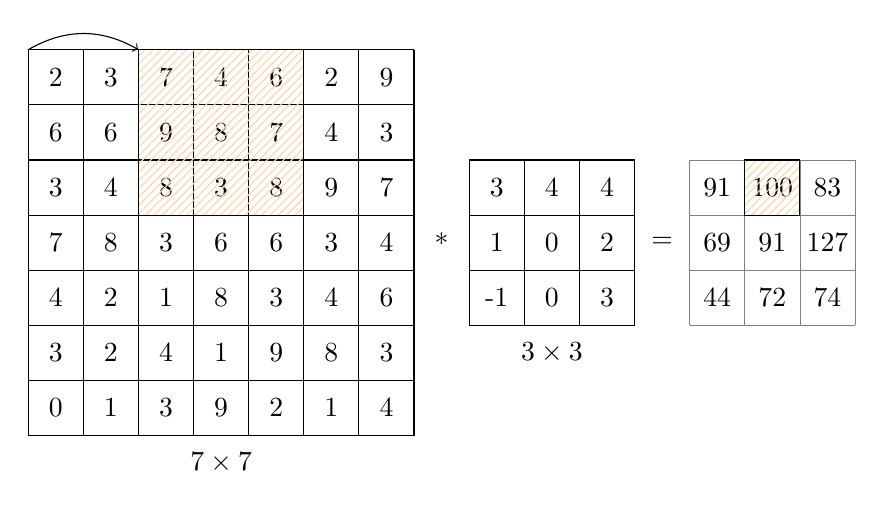
\begin{tikzpicture}[scale=0.7]       
      \draw[step=1cm] (0, 0) grid (7, 7);
      % Starting from bottom row, working left to right.
      \node at (0.5, 0.5) {0};
      \node at (1.5, 0.5) {1};
      \node at (2.5, 0.5) {3};
      \node at (3.5, 0.5) {9};
      \node at (4.5, 0.5) {2};
      \node at (5.5, 0.5) {1};
      \node at (6.5, 0.5) {4};
      % second row from bottom.
      \node at (0.5, 1.5) {3};
      \node at (1.5, 1.5) {2};
      \node at (2.5, 1.5) {4};
      \node at (3.5, 1.5) {1};
      \node at (4.5, 1.5) {9};
      \node at (5.5, 1.5) {8};
      \node at (6.5, 1.5) {3};
      % Third from bottom.
      \node at (0.5, 2.5) {4};
      \node at (1.5, 2.5) {2};
      \node at (2.5, 2.5) {1};
      \node at (3.5, 2.5) {8};
      \node at (4.5, 2.5) {3};
      \node at (5.5, 2.5) {4};
      \node at (6.5, 2.5) {6};
      % Fourth from bottom.
      \node at (0.5, 3.5) {7};
      \node at (1.5, 3.5) {8};
      \node at (2.5, 3.5) {3};
      \node at (3.5, 3.5) {6};
      \node at (4.5, 3.5) {6};
      \node at (5.5, 3.5) {3};
      \node at (6.5, 3.5) {4};
      % Fifth from bottom
      \node at (0.5, 4.5) {3};
      \node at (1.5, 4.5) {4};
      \node at (2.5, 4.5) {8};
      \node at (3.5, 4.5) {3};
      \node at (4.5, 4.5) {8};
      \node at (5.5, 4.5) {9};
      \node at (6.5, 4.5) {7};
      % Second from top.
      \node at (0.5, 5.5) {6};
      \node at (1.5, 5.5) {6};
      \node at (2.5, 5.5) {9};
      \node at (3.5, 5.5) {8};
      \node at (4.5, 5.5) {7};
      \node at (5.5, 5.5) {4};
      \node at (6.5, 5.5) {3};
      % Top row.
      \node at (0.5, 6.5) {2};
      \node at (1.5, 6.5) {3};
      \node at (2.5, 6.5) {7};
      \node at (3.5, 6.5) {4};
      \node at (4.5, 6.5) {6};
      \node at (5.5, 6.5) {2};
      \node at (6.5, 6.5) {9};
      \node at (3.5, -.5) {$7 \times 7$};
      \node at (7.5, 3.5) {*};
      \filldraw[pattern=north east lines, pattern color = orange!33] (2, 4) rectangle (5,7);
      % Filter
      \draw[step=1cm] (8, 2) grid (11, 5);
      % Bottom row of filter.
      \node at (8.5, 2.5) {-1};
      \node at (9.5, 2.5) {0};
      \node at (10.5, 2.5) {3};
      % Middle row of filter.
      \node at (8.5, 3.5) {1};
      \node at (9.5, 3.5) {0};
      \node at (10.5, 3.5) {2};
      % Top row of filter.
      \node at (8.5, 4.5) {3};
      \node at (9.5, 4.5) {4};
      \node at (10.5, 4.5) {4};
      \node at (11.5, 3.5) {=};
      \node at (9.5, 1.5) {$3 \times 3$};
      \draw[step=1cm,gray, very thin] (12, 2) grid (15, 5);
      \node at (12.5, 4.5) {91};
      \node at (13.5, 4.5) {100};
      \node at (14.5, 4.5) {83};
      \node at (12.5, 3.5) {69};
      \node at (13.5, 3.5) {91};
      \node at (14.5, 3.5) {127};
      \node at (12.5, 2.5) {44};
      \node at (13.5, 2.5) {72};
      \node at (14.5, 2.5) {74};
      \filldraw[pattern=north east lines, pattern color = orange!33] (13, 4) rectangle (14,5);
      \path[->] (0, 7) edge[bend left] (2, 7);
  \end{tikzpicture}
  \caption{\footnotesize An example of stride-length of size two. We highlight how we calculate the element in the output residing
in the second column of the first row. Similar rules apply when we wish to obtain the elements from the second row: we will slide our filter down by two positions
before taking an element-wise product and summing.}
\end{figure}

\subsubsection{Dimension for padded images with stride}
In general, if we have an $n \times n$ input matrix, an $f \times f$ filter, padding of size $p$, and a stride-length of $s$,
the number of elements in the output is
\begin{equation*}   \left(\floor{\frac{n + 2p - f}{s} + 1}\right) \times \left(\floor{\frac{n + 2p - f}{s} + 1}\right) \end{equation*}
We've taken the floor operation $\floor{\cdot}$ to ensure that if our stride-length doesn't evenly divide
our (padded) input matrix that we still have an output with well defined dimension.\footnote{
There is one more point worth mentioning: some fields mirror the filter by flipping once in each direction (with the first flip, the first row becomes the first column, and with the second flip this first column becomes the last row with the elements reversed). In the deep learning community, this is not often done; it's worth knowing that this technique is
known as cross-correlation.}

\subsection{Convolutions over Volume} Let's consider a convolution over 3D volumes. Suppose we have a $6 \times 6$ matrix
which encodes the RGB representation of the image. We can actually think about this as a ``stack of matrices''.

\begin{figure}[h]   \centering
  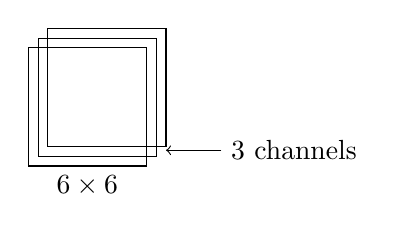
\begin{tikzpicture}[scale=0.5]     \draw (0.5, 0.5) rectangle (3.5, 3.5);     \draw (0.25, 0.25) rectangle (3.25, 3.25); 
    \draw (0, 0) rectangle (3, 3);
    \node at (1.5, -.5) {$6 \times 6$};
    \node (channels) at (6.75, .4) {$3$ channels};
    \draw[->] (channels) to (3.5, .4);
  \end{tikzpicture} \end{figure}

In order to detect edges (or some other feature) in this image, you can convolve this with a 3D filter (e.g. a $3 \times 3 \times 3$ kernel); the filter itself will have one layer for each of the three RGB channels.

\begin{figure}[h]   
  \centering
  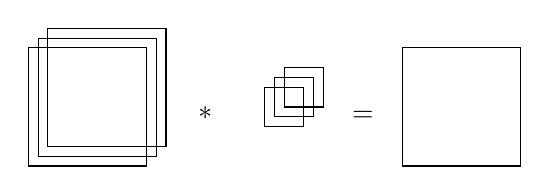
\begin{tikzpicture}[scale=0.5]
    \draw (0.5, 0.5) rectangle (3.5, 3.5);     
    \draw (0.25, 0.25) rectangle (3.25, 3.25); 
    \draw (0, 0) rectangle (3, 3);
    \node at (4.5, 1.25) {*};
    \draw (6.5, 1.5) rectangle (7.5, 2.5);     
    \draw (6.25, 1.25) rectangle (7.25, 2.25); 
    \draw (6, 1) rectangle (7, 2);
    \node at (8.5, 1.25) {=};
    \draw (9.5, 0) rectangle (12.5, 3);
  \end{tikzpicture}
  \caption{Note that when we apply a three-dimensional convolution to our image, the output no longer has a third dimension.}
\end{figure}

\paragraph{Terminology} The input image is $6 \times 6 \times 3$, where we say the first dimensions corresponds to the \emph{height}
of the image, the second corresponds to the \emph{width} of the image, and the last corresponds to the \emph{number of channels}. 
Of course, the filter itself also has height, width, and a number of channels.  Note that we \emph{require} that the number
of channels in the input image match the number of channels in the filter.

\begin{figure}[h]   \centering
  \begin{tikzpicture}       \draw[ultra thick, draw = black, fill = blue ] (0.5, 0.5) grid (5.5, 5.5) rectangle (0.5, 0.5);     
      \draw[ultra thick, draw = black, fill = green] (0.25, 0.25) grid (5.25, 5.25) rectangle (0.25, 0.25);     
      \draw[ultra thick, draw = black, fill = red  ] (0, 0) grid (5, 5) rectangle (0, 0);    
      \node at (6.25, 3) {*};
      \draw[step = 0.5cm, ultra thick, draw = black, fill = yellow] (8, 3.5) grid (9.5, 5) rectangle (8, 3.5); 
      \draw[step = 0.5cm, ultra thick, draw = black, fill = yellow] (7.5, 3) grid (9, 4.5) rectangle (7.5, 3);       \draw[step = 0.5cm, ultra thick, draw = black, fill = yellow] (7, 2.5) grid (8.5, 4) rectangle (7, 2.5); 
      \node at (10, 3) {=};
      \draw[step = 0.5cm, ultra thick, draw = black] (10.99, 1.99) grid (13, 4);
    \end{tikzpicture}
    \caption{\footnotesize To compute the output of a three-dimensional convolution, we can first perform element-wise multiplications
      for each filter with its corresponding channel in the original input image; then, we sum up all the elements together
      to yield a single scalar value. We then slide our convolution over one position and repeat the process until we've applied
      our filter across the extents of the input image.} \end{figure}

What does having a three-dimensional convolution allow us to do? Suppose we want to detect vertical edges in the red channel
of the image only. Then, we'd choose our three-dimensional filter to look like
\begin{figure}[h]
  \centering   \begin{tikzpicture}
    \node at (0, 1.75) {R};     \draw[step = 0.5cm, ultra thick, draw = black] (0, 0) grid (1.5, 1.5);
    \node at (0.25, 0.25) {1};
    \node at (0.25, 0.75) {1};
    \node at (0.25, 1.25) {1};
    \node at (0.75, 0.25) {0};
    \node at (0.75, 0.75) {0};
    \node at (0.75, 1.25) {0};
    \node at (1.25, 0.25) {-1};
    \node at (1.25, 0.75) {-1};
    \node at (1.25, 1.25) {-1};
    \node at (2, 1.75) {G};
    \draw[step = 0.5cm, ultra thick, draw = black] (1.99, 0) grid (3.5, 1.5);
    \node at (2.25, 0.25) {0};
    \node at (2.25, 0.75) {0};
    \node at (2.25, 1.25) {0};
    \node at (2.75, 0.25) {0};
    \node at (2.75, 0.75) {0};
    \node at (2.75, 1.25) {0};
    \node at (3.25, 0.25) {0};
    \node at (3.25, 0.75) {0};
    \node at (3.25, 1.25) {0};
    \node at (4, 1.75) {B};
    \draw[step = 0.5cm, ultra thick, draw = black] (3.99, 0) grid (5.5, 1.5);
    \node at (4.25, 0.25) {0};
    \node at (4.25, 0.75) {0};
    \node at (4.25, 1.25) {0};
    \node at (4.75, 0.25) {0};
    \node at (4.75, 0.75) {0};
    \node at (4.75, 1.25) {0};
    \node at (5.25, 0.25) {0};
    \node at (5.25, 0.75) {0};
    \node at (5.25, 1.25) {0};
  \end{tikzpicture}
  \caption{\footnotesize A 3-D filter for detecting vertical edges in the red channel of an image. If we wanted to detect vertical
    edges in any color channel, we can use edge detectors in each of the channels (i.e. making each filter identical 
    to the red channel above).} \end{figure}

\paragraph{Using multiple filters} What if we wanted to detected not only vertical edges, but also edges of various orientations
as well, i.e. what if we wanted to use multiple filters at the same time? There is a natural way to achieve this goal that yields
an output that is 3-D. Let's consider an example where we have two filters.

\begin{figure}[h]   
  \centering
  \begin{tikzpicture}       
    \draw[ultra thick, draw = black, fill = blue ] (0.5, 0.5) grid (5.5, 5.5) rectangle (0.5, 0.5);     
    \draw[ultra thick, draw = black, fill = green] (0.25, 0.25) grid (5.25, 5.25) rectangle (0.25, 0.25);     
    \draw[ultra thick, draw = black, fill = red  ] (0, 0) grid (5, 5) rectangle (0, 0);    
    \node at (6.25, 4) {*};
    \node at (8.75, 6.5) {$\substack{\footnotesize{\textrm{vertical}} \\ \footnotesize{\textrm{edge-detector}}}$};
    \draw[step = 0.5cm, ultra thick, draw = black, fill = yellow] (8, 4.5) grid (9.5, 6) rectangle (8, 4.5); 
    \draw[step = 0.5cm, ultra thick, draw = black, fill = yellow] (7.5, 4) grid (9, 5.5) rectangle (7.5, 4);       
    \draw[step = 0.5cm, ultra thick, draw = black, fill = yellow] (7, 3.5) grid (8.5, 5) rectangle (7, 3.5); 
    \node at (6.25, 2) {*};
    \node at (8.75, 3) {$\substack{\footnotesize{\textrm{horizontal}} \\ \footnotesize{\textrm{edge-detector}}}$};
    \draw[step = 0.5cm, ultra thick, draw = black, fill = orange] (8, 1)      grid (9.5, 2.5) rectangle (8, 1); 
    \draw[step = 0.5cm, ultra thick, draw = black, fill = orange] (7.49, 0.5) grid (9, 2)     rectangle (7.49, 0.5);       
    \draw[step = 0.5cm, ultra thick, draw = black, fill = orange] (7, 0)      grid (8.5, 1.5) rectangle (7, 0); 
    \node at (10, 2) {=};
    \node at (10, 5) {=};
    \draw[step = 0.5cm, ultra thick, draw = purple] (10.99, 3.99) grid (13, 6);
    \draw[step = 0.5cm, ultra thick, draw = blue  ] (10.99, .99) grid (13, 3);
    % superimposition to get a 3-d output.
    \draw[purple] (14, 3) rectangle (16, 5);
    \draw[blue] (13.7, 2.7) rectangle (15.7, 4.7);
    \draw[->,purple] (13, 6) -- (14, 5);
    \draw[->,blue] (13, 3) -- (13.7, 2.7);
  \end{tikzpicture}
  \caption{\footnotesize To apply multiple filters simultaneously, we first apply each filter to the input image and obtain an output. We then ``stack'' these outputs into a new stack of matrices. In this example, we've computed both vertical and horizontal edge detectors which each yield 2-D outputs of the same size which can be combined in a final step.} 
\end{figure}

\subsubsection{Dimension of output from 3-D convolution without padding and unit stride length} 
If you have an $n \times n \times n_c$ where $n_c$ denotes the number of channels,
and we convolve it with an $f \times f \times n_c$, we yield an output of size $(n-f+1) \times (n-f+1) \times n_f$
where $n_f$ denotes the number of filters we wish to apply. Note that we've assumed no padding and unit stride-length.
In deep learning literature, $n_f$ is often referred to as the depth of the 3-D volume.

\subsubsection{One layer of a CNN}

\begin{figure}[h]   
  \centering
  \begin{tikzpicture}[scale=0.8]       
    \draw[ultra thick, draw = black, fill = blue ] (0.5, 0.5) grid (5.5, 5.5) rectangle (0.5, 0.5);     
    \draw[ultra thick, draw = black, fill = green] (0.25, 0.25) grid (5.25, 5.25) rectangle (0.25, 0.25);     
    \draw[ultra thick, draw = black, fill = red  ] (0, 0) grid (5, 5) rectangle (0, 0);
    \draw [decorate,decoration={brace,amplitude=10pt,mirror}] (0,-0.5) -- (5.5, -0.5) node[midway,below,yshift=-.4cm] {``$a^{[0]}$''};
    \node at (6.25, 4) {*};
    \node at (8.75, 6.5) {$\substack{\footnotesize{\textrm{vertical}} \\ \footnotesize{\textrm{edge-detector}}}$};
    \draw[step = 0.5cm, ultra thick, draw = black, fill = yellow] (8, 4.5) grid (9.5, 6) rectangle (8, 4.5); 
    \draw[step = 0.5cm, ultra thick, draw = black, fill = yellow] (7.5, 4) grid (9, 5.5) rectangle (7.5, 4);       
    \draw[step = 0.5cm, ultra thick, draw = black, fill = yellow] (7, 3.5) grid (8.5, 5) rectangle (7, 3.5); 
    \node at (6.25, 2) {*};
    \node at (8.75, 3) {$\substack{\footnotesize{\textrm{horizontal}} \\ \footnotesize{\textrm{edge-detector}}}$};
    \draw[step = 0.5cm, ultra thick, draw = black, fill = orange] (8, 1)      grid (9.5, 2.5) rectangle (8, 1); 
    \draw[step = 0.5cm, ultra thick, draw = black, fill = orange] (7.49, 0.5) grid (9, 2)     rectangle (7.49, 0.5);       
    \draw[step = 0.5cm, ultra thick, draw = black, fill = orange] (7, 0)      grid (8.5, 1.5) rectangle (7, 0); 
    \draw [decorate,decoration={brace,amplitude=10pt,mirror}] (7,-0.5) -- (9.5, -0.5) node[midway,below,yshift=-.4cm] {``$W^{[1]}$''};
    \node at (10, 2) {=};
    \node at (10, 5) {=};
    \node at (11, 2) {\textrm{ReLU} $\bigg($};
    \node at (11, 5) {\textrm{ReLU} $\bigg($};
    \draw[step = 0.5cm, ultra thick, draw = purple] (11.99, 3.99) grid (14, 6);
    \draw[step = 0.5cm, ultra thick, draw = blue  ] (11.99, .99) grid (14, 3);
    \draw [decorate,decoration={brace,amplitude=10pt,mirror}] (11.99,0.75) -- (14, 0.75) node[midway,below,yshift=-.4cm] {``$W^{[1]} a^{[0]}$''};
    \node at (14.5, 2) {$+ b_2$};
    \node at (14.5, 5) {$+ b_1$};
    \node at (15, 2) {$\bigg)$};
    \node at (15, 5) {$\bigg)$};
    \draw[purple] (16,     3) rectangle (18, 5);
    \draw[blue]   (15.7, 2.7) rectangle (17.7, 4.7);
    \draw[->, purple] (15.1, 5.1) -- (15.9, 5);
    \draw[->, blue  ] (15.1, 2.1) -- (15.6, 2.7);
    \draw [decorate,decoration={brace,amplitude=10pt,mirror}] (10.5,-0.5) -- (15, -0.5) node[midway,below,yshift=-.4cm] {``$Z^{[1]}$''};
    \draw [decorate,decoration={brace,amplitude=10pt,mirror}] (15.75,2.7) -- (18, 2.7) node[midway,below,yshift=-.4cm] {``$a^{[1]}$''};
  \end{tikzpicture}
  \caption{\footnotesize Here we relate parameters of a CNN to what we've seen previously. Our input image, sometimes demoted
by $X$, is really the zeroth activation. We then have filters which act as weight matrices, and we compute $W^{[1]} a^{[0]} + b_i$
which is a \emph{linear} function. To incorporate non-linearity, we choose an appropriate activation function, and computing this
gives us the analogous $Z^{[1]} = \texttt{ReLU}(W^{[1]} a^{[0]} + b_i)$. As a last step, we combine or stack the outputs into a tensor.}
\end{figure}

If we want, we can think about a mapping from a 3-D volume $A^{[0]}$, our input image, into another 3-D volume which is $A^{[1]}$,
the output of the first layer.
\begin{figure}[h]   \centering   \begin{tikzpicture}[scale=0.5]
    \pgfmathsetmacro{\cubex}{2} 
    \pgfmathsetmacro{\cubey}{1} 
    \pgfmathsetmacro{\cubez}{1}
    \node at (-2, -1.25) {$a^{[0]}$}; 
    \draw[black] (0,0,0) -- ++(-\cubex,0,0) -- ++(0,-\cubey,0) -- ++(\cubex,0,0) -- cycle; 
    \draw[black] (0,0,0) -- ++(0,0,-\cubez) -- ++(0,-\cubey,0) -- ++(0,0,\cubez) -- cycle; 
    \draw[black] (0,0,0) -- ++(-\cubex,0,0) -- ++(0,0,-\cubez) -- ++(\cubex,0,0) -- cycle; 
    \draw[->] (1, 0, 1) -- (2, 0, 1);
    \node at (3, -1.25) {$a^{[1]}$}; 
    \draw[black] (3,0,0) -- ++(-\cubex/2,0,0) -- ++(0,-\cubey,0) -- ++(\cubex/2,0,0) -- cycle; 
    \draw[black] (3,0,0) -- ++(0,0,-\cubez) -- ++(0,-\cubey,0) -- ++(0,0,\cubez) -- cycle; 
    \draw[black] (3,0,0) -- ++(-\cubex/2,0,0) -- ++(0,0,-\cubez) -- ++(\cubex/2,0,0) -- cycle; 
  \end{tikzpicture}
  \caption{\footnotesize We can think about each layer as transforming one 3-D volume into another.}
\end{figure}

\paragraph{Example: \# parameters in a 3-D convolution with multiple filters} If we have 10 filters that are each $3 \times 3 \times 3$ in one layer of a neural network, how many
parameters does that layer have? Each filter contains $3^3 = 27$ parameters we need to learn, plus a bias term yielding a total of 
28 learnable parameters per filter. With 10 filters, we have a total of 280 parameters in the first layer of our neural network.
Notice that the number of parameters we have to learn \emph{does not} depend on the size of the input. This is a property of CNN's: so long as you learn feature detectors that work, you can apply this to very large images while keeping the number of parameters fixed and relatively small.

\subsubsection{Notation for CNN's}
We will say that
\begin{align*}   f^{[\ell]} &= \textrm{filter size} \\
  p^{[\ell]} &= \textrm{padding} \\
  s^{[\ell]} &= \textrm{stride} \end{align*}
The input has dimension $n \times n \times n_c$ where recall $n_c$ is the number of channels. To generalize the notation to a 
deep neural network, we add superscript square brackets to indicate what layer we're examining. Further, our images might not be square, so we add subscripts to indicate whether we are referring to height or width. I.e. we say that the input
to each layer can be described by
\[
n_H^{[\ell-1]} \times n_W^{[\ell-1]} \times n_c^{[\ell-1]}.
\]

\subsubsection{Output volume size: general formula}
Note that the output volume size is given by 
\[
n_H^{[\ell]} = \floor{\frac{n_H^{[\ell-1]} + 2p^{[\ell]} - f^{[\ell]}}{s^{[\ell]}} + 1}
\]
The same is true for the width, replacing $n_H$ with $n_W$ in the formula above. Note that $n_c^{[\ell]}$, the number of channels in layer $\ell$ of the network, is given by the number of filters we are applying in the previous layer.
Each filter is size $f^{[\ell]} \times f^{[\ell]} \times n_c^{[\ell-1]}$. Activations will be of dimension $a^{[\ell]} = n_H^{[\ell]} \times n_W^{[\ell]} \times n_c^{[\ell]}$. If we're using vectorized implementation, e.g. batch gradient descent, we have
\[
A^{[\ell]} = m \times n_H^{[\ell]} \times n_W^{[\ell]} \times n_c^{[\ell]}.
\]

\subsubsection{Number of learnable parameters for 3-D convolutions}
Next, consider the weights. We've mentioned above that the dimension of a single filter is $f^{[\ell]} \times f^{[\ell]} \times n_c^{[\ell-1]}$, so to get the total number of weights we need 
\[
\left(f^{[\ell]} \times f^{[\ell]} \times n_c^{[\ell-1]} + 1 \right) \times n_c^{[\ell]}
\]
where the last term is synonymous with the number of filters in layer $\ell$.
Lastly, consider the bias parameters. We have a single scalar value \emph{for each filter}. The bias will be a vector of dimension $n_c^{[\ell]}$.\footnote{Note that the order of height, width, then channel is arbitrary and different authors in the deep learning community use different conventions. They key is to be consistent, in spite of there not being consensus in the deep learning literature.}

\subsection{Deep convolutional neural network example} Suppose we have an image and we want to perform image recognition, e.g.
does the picture contain a cat? Suppose our input is size $39 \times 39 \times 3$. This means that 
\begin{align*}   
  n_H^{[0]} &= n_W^{[0]} = 39 \\
  n_c^{[0]} &= 3 
\end{align*}
Let's say the first layer uses a set of $3 \times 3$ filters to detect features, and further suppose we have unit stride length
and no padding. Further suppose that you have 10 filters. Then, we have the following transformation:
\begin{figure}[h]   \centering
  \begin{tikzpicture}[scale=0.9]     \pgfmathsetmacro{\cubex}{2} 
    \pgfmathsetmacro{\cubey}{1} 
    \pgfmathsetmacro{\cubez}{1}
    \node at (-1, -1.25) {$39 \times 39 \times 3$}; 
    \node at (-1, -2)  {$n_H^{[0]} = n_W^{[0]} = 39$};
    \node at (-1, -2.75) {$n_c^{[0]} = 3$};
    \draw[black] (0,0,0) -- ++(-\cubex,0,0) -- ++(0,-\cubey,0) -- ++(\cubex,0,0) -- cycle; 
    \draw[black] (0,0,0) -- ++(0,0,-\cubez) -- ++(0,-\cubey,0) -- ++(0,0,\cubez) -- cycle; 
    \draw[black] (0,0,0) -- ++(-\cubex,0,0) -- ++(0,0,-\cubez) -- ++(\cubex,0,0) -- cycle; 
    \draw[->] (1, 0, 1) -- (4, 0, 1) node[below left] {$\substack{f^{[1]} = 3 \\ s^{[1]} = 1 \\ p^{[1]} = 0 \\ \textrm{10 filters}}$};
    \draw[black] (6,0,0) -- ++(-\cubex/2,0,0) -- ++(0,-\cubey,0) -- ++(\cubex/2,0,0) -- cycle; 
    \draw[black] (6,0,0) -- ++(0,0,-\cubez) -- ++(0,-\cubey,0) -- ++(0,0,\cubez) -- cycle; 
    \draw[black] (6,0,0) -- ++(-\cubex/2,0,0) -- ++(0,0,-\cubez) -- ++(\cubex/2,0,0) -- cycle;
    \node at (6, -1, 0.5) {$37 \times 37 \times 10$};
    \node at (6, -1.5, 0.5) {$n_H^{[1]} = n_W^{[1]} = 37$};
    \node at (6, -2, 0.5) {$n_c^{[1]} = 10$};   \end{tikzpicture} \end{figure}

Notice that the 37 comes from the formula $\floor{\frac{n + 2p - f}{s} + 1} = \floor{\frac{39 + 0 - 3}{1} + 1} = 37$.
Further realize this is a Valid convolution. In this example, $n_H^{[1]} = n_W^{[1]} = 37$, and $n_c^{[1]} = 10$ since we have
10 filters. We know now the dimensions of the activation at the first layer.
Note that $f^{[1]} = 3$ simply because we're using $3 \times 3$ filters. 

\paragraph{Adding another convolution layer}
Let's say we have another convolution layer, but this time we're using $5 \times 5$ filters; in our notation $f^{[2]} = 5$. Further,
we're also going to use a stride-length of two, no padding, and twenty filters.

\begin{figure}[h]   
  \centering
  \begin{tikzpicture}[scale=0.9]     
    \pgfmathsetmacro{\cubex}{2} 
    \pgfmathsetmacro{\cubey}{1} 
    \pgfmathsetmacro{\cubez}{1}
    \node at (-1, -1.25) {$39 \times 39 \times 3$}; 
    \node at (-1, -2)  {$n_H^{[0]} = n_W^{[0]} = 39$};
    \node at (-1, -2.75) {$n_c^{[0]} = 3$};
    \draw[black] (0,0,0) -- ++(-\cubex,0,0) -- ++(0,-\cubey,0) -- ++(\cubex,0,0) -- cycle; 
    \draw[black] (0,0,0) -- ++(0,0,-\cubez) -- ++(0,-\cubey,0) -- ++(0,0,\cubez) -- cycle; 
    \draw[black] (0,0,0) -- ++(-\cubex,0,0) -- ++(0,0,-\cubez) -- ++(\cubex,0,0) -- cycle; 
    \draw[->] (1, 0, 1) -- (4, 0, 1) node[below left] {$\substack{f^{[1]} = 3 \\ s^{[1]} = 1 \\ p^{[1]} = 0 \\ \textrm{10 filters}}$};
    \draw[black] (6,0,0) -- ++(-\cubex/2,0,0) -- ++(0,-\cubey,0) -- ++(\cubex/2,0,0) -- cycle; 
    \draw[black] (6,0,0) -- ++(0,0,-\cubez) -- ++(0,-\cubey,0) -- ++(0,0,\cubez) -- cycle; 
    \draw[black] (6,0,0) -- ++(-\cubex/2,0,0) -- ++(0,0,-\cubez) -- ++(\cubex/2,0,0) -- cycle;
    \node at (6, -1.1, 0.5) {$37 \times 37 \times 10$};
    \node at (6, -1.6, 0.5) {$n_H^{[1]} = n_W^{[1]} = 37$};
    \node at (6, -2.1, 0.5) {$n_c^{[1]} = 10$};   
    \draw[black] (11,0,0) -- ++(-\cubex/3,0,0) -- ++(0,-\cubey,0) -- ++(\cubex/3,0,0) -- cycle; 
    \draw[black] (11,0,0) -- ++(0,0,-\cubez) -- ++(0,-\cubey,0) -- ++(0,0,\cubez) -- cycle; 
    \draw[black] (11,0,0) -- ++(-\cubex/3,0,0) -- ++(0,0,-\cubez) -- ++(\cubex/3,0,0) -- cycle;
    \draw[->] (7, 0, 1) -- (10.5, 0, 1) node[below left] {$\substack{f^{[2]} = 5 \\ s^{[2]} = 2 \\ p^{[2]} = 0 \\ \textrm{20 filters}}$};
    \node at (13, 0, 0) {$17 \times 17 \times 20$};
    \node at (13, -.75, 0) {$n_H^{[2]} = n_W^{[2]} = 17$};
    \node at (13, -1.5, 0) {$n_c^{[2]} = 20$};
  \end{tikzpicture} 
\end{figure}
Notice that because we used a stride-length of two on the second layer, that the size of our input shrunk very fast, it went from
$39 \leadsto 17$; since we're using twenty channels, we have the last dimension as 20.

\paragraph{Final convolution and transformation into fitted probabilities}
Lastly, let's apply one more convolution. We'll again use a $5 \times 5$ filter and so
$f^{[3]} = 5$. We will use a stride length of $2$ and fourty filters with no padding. The math works out 
such that we output a $7 \times 7 \times 40$ \emph{features} describing a 3-D volume. What's commonly done 
next is to realize that $7 \times 7 \times 40 = 1,960$, and so we can unravel our 3-D data structure
into a nice long vector, which can then be fed as input into a logistic regression or softmax unit.

\paragraph{Trends in ConvNets} As you go deeper into a neural network, the height and width of the input shrinks gradually; on
the other hand, the number of channels will generally increase. 

\subsection{Pooling Layers} Other than convolutional layers, ConvNets also often use pooling to reduce the size of the representation, to speed up computation, and to make some of the features more robust. We start with an example which motivates why we might
want to consider a pooling strategy. We start by taking our $4 \times 4$ input and breaking it into different regions. The output will be $2 \times 2$ and each cell will take on the max value of the corresponding region in the input.

\begin{figure}[h]
  \centering   \begin{tikzpicture}
    \draw[ultra thick, draw = black, fill=purple] (0,0) grid (2,2) rectangle (0,0);
    \draw[ultra thick, draw = black, fill=blue]   (0,2) grid (2,4) rectangle (0,2);
    \draw[ultra thick, draw = black, fill=green]  (2,0) grid (4,2) rectangle (2,0);
    \draw[ultra thick, draw = black, fill=orange] (2,2) grid (4,4) rectangle (2,2);
    \node at (0.5, 0.5) {5};
    \node at (1.5, 0.5) {6};
    \node at (0.5, 1.5) {1};
    \node at (1.5, 1.5) {3};
    \node at (2.5, 0.5) {1};
    \node at (3.5, 0.5) {2};
    \node at (2.5, 1.5) {2};
    \node at (3.5, 1.5) {3};
    \node at (0.5, 2.5) {2};
    \node at (1.5, 2.5) {9};
    \node at (0.5, 3.5) {1};
    \node at (1.5, 3.5) {3};
    \node at (2.5, 2.5) {1};
    \node at (2.5, 3.5) {2};
    \node at (3.5, 2.5) {1};
    \node at (3.5, 3.5) {1}; 
    \draw[->] (5, 2) -- (7, 2) node[align=center, above left] {\textrm{Max-pooling}};
    \draw[ultra thick, draw=black, fill = purple] (8,1) grid (9, 2) rectangle (8,1);
    \node at (8.5, 1.5) {6};
    \draw[ultra thick, draw=black, fill = green] (9,1) grid (10, 2) rectangle (9,1);
    \node at (9.5, 1.5) {3};
    \draw[ultra thick, draw=black, fill = blue] (8,2) grid (9, 3) rectangle (8,2);
    \node at (8.5, 2.5) {9};
    \draw[ultra thick, draw=black, fill = orange] (9,2) grid (10, 3) rectangle (9,2);
    \node at (9.5, 2.5) {2};
  \end{tikzpicture}
  \caption{With max-pooling, we partition our input and then take the maximum value within each
    disjoint set of elements. In the example above, it's as if we applied a filter of size two,
since we're taking $2 \times 2$ regions and using a stride-length of two. Filter size and stride length
are hyperparameters of max pooling.} \end{figure}

\paragraph{Intuition behind max-pool} If you consider the $4 \times 4$ region as a set of features or activations in the network,
then a large number means it has perhaps detected a particular feature. E.g. the upper-left quadrant maybe capturing a vertical edge, or a whisker if we're trying to detect a cat. Max pooling effectively preserves detected features through to the subsequent layer.

\paragraph{Gradient descent and max pooling} It's interesting to note that max-pooling has a set of hyperparameters, but it has no
parameters to learn. Once the filter size $f$ and stride length $s$ are fixed, there's nothing to learn; it's just a fixed 
computation. The same formulae apply for dimensions, where the size of the subsequent layer is given by $\floor{\frac{n+2p - f}{s} + 1}$. If you have an image with multiple channels, then the output of the max-pooling operation will have just as many channels.
The way it works is that we apply max-pooling to each channel independently and write the results to a table; finally, we can stack up the results into a 3-D data structure.

\paragraph{Average pooling} This is exactly what you would expect. Max pooling is used much more often with one exception:
sometimes very deep in a neural network you may wish to collapse your representation.

\paragraph{Common choices of hyperparameters} Many set $f=2$ and $s=2$, and this has the effect of roughly halving the height and width of the representation by a factor of two. When you do max-pooling, you usually \emph{never} pad. It's reasonable to try a few values of these hyperparameters and see which works best by cross-validation.

\subsection{Convolutional neural nets for digit recognition} 
We now have the building blocks for constructing a full convolutional neural network, and so we next
consider an example. Suppose you're given an input image with dimension $32 \times 32 \times 3$, i.e. an RGB image, and you would
like to perform handwritten digit recognition. E.g. maybe we have a number like seven in a $32 \times 32$ RGB image.
\begin{figure}[h]   \centering
  \begin{tikzpicture}[scale=0.5]     \draw (0.5, 0.5)   rectangle (3.5, 3.5);     
    \draw (0.25, 0.25) rectangle (3.25, 3.25); 
    \draw (0, 0)       rectangle (3, 3);    
    \node at (1.5, 1.5) {7};   \end{tikzpicture} \end{figure}
We'd like to recognize which of the digits in the set $\{0, 1, \ldots, 9\}$ this image contains. We're going to implement a neural
network inspired by \href{http://yann.lecun.com/exdb/lenet/}{LeNet-5}, which itself was created by 
\href{http://yann.lecun.com/}{Yann LeCun}. Suppose that for the first layer we use a $5 \times 5$ filter and unit stride-length
with no padding. From our formula we know the output will be $n-f+1 \leadsto 28 \times 28$, and if we use 6 filters our output from
the first layer will be $28 \times 28 \times 6$. We'll call this first layer \texttt{Conv1}: it's the result of applying six filters, adding a bias, then applying a non-linearity.

\begin{figure}[h]
  \centering   \begin{tikzpicture}
    \pgfmathsetmacro{\cubex}{2} 
    \pgfmathsetmacro{\cubey}{1} 
    \pgfmathsetmacro{\cubez}{1}
    \node at (-2, -1.25) {$\scriptstyle 32 \times 32 \times 3$}; 
    \draw[black] (-1,0,0) -- ++(-\cubex,0,0) -- ++(0,-\cubey,0) -- ++(\cubex,0,0) -- cycle; 
    \draw[black] (-1,0,0) -- ++(0,0,-\cubez) -- ++(0,-\cubey,0) -- ++(0,0,\cubez) -- cycle; 
    \draw[black] (-1,0,0) -- ++(-\cubex,0,0) -- ++(0,0,-\cubez) -- ++(\cubex,0,0) -- cycle; 
    \draw[->] (-.5, 0, 1) -- (1, 0, 1) node[below left] {$\substack{f = 5 \\ s = 1 \\ p = 0 \\ \textrm{6 filters}}$};
    \draw[black] (1.75,0,0) -- ++(-\cubex/2,0,0) -- ++(0,-\cubey,0) -- ++(\cubex/2,0,0) -- cycle; 
    \draw[black] (1.75,0,0) -- ++(0,0,-\cubez) -- ++(0,-\cubey,0) -- ++(0,0,\cubez) -- cycle; 
    \draw[black] (1.75,0,0) -- ++(-\cubex/2,0,0) -- ++(0,0,-\cubez) -- ++(\cubex/2,0,0) -- cycle;
    \node at (1.75, 1, 0.5) {\texttt{Conv1}};
    \node at (1.75, -1.1, 0.5) {$\scriptstyle 28 \times 28 \times 6$};
    \draw[->] (2, 0, 1) -- (4.25, 0, 1) node[below left] {$\substack{\texttt{max-pool} \\ f = 2 \\ s = 2 \\ p = 0}$};
    \draw[black] (5,0,0) -- ++(-\cubex/2,0,0) -- ++(0,-\cubey,0) -- ++(\cubex/2,0,0) -- cycle; 
    \draw[black] (5,0,0) -- ++(0,0,-\cubez) -- ++(0,-\cubey,0) -- ++(0,0,\cubez) -- cycle; 
    \draw[black] (5,0,0) -- ++(-\cubex/2,0,0) -- ++(0,0,-\cubez) -- ++(\cubex/2,0,0) -- cycle;
    \node at (5, -1.1, 0.5) {$\scriptstyle 14 \times 14 \times 6$};
    \node at (5, 1, .5) {\texttt{Pool1}};
    \draw [decorate,decoration={brace,amplitude=10pt,mirror}] (0.5,-1.7) -- (5.6, -1.7) node[midway,below,yshift=-.4cm] {\texttt{Layer 1}};
    \draw[->] (6, 0, 1) -- (7.5, 0, 1) node[below left] {$\substack{f=5 \\ s = 1 \\ p = 0 \\ \textrm{16 filters}}$};
    \draw[black] (8.5,0,0) -- ++(-\cubex/2,0,0) -- ++(0,-\cubey,0) -- ++(\cubex/2,0,0) -- cycle; 
    \draw[black] (8.5,0,0) -- ++(0,0,-\cubez) -- ++(0,-\cubey,0) -- ++(0,0,\cubez) -- cycle; 
    \draw[black] (8.5,0,0) -- ++(-\cubex/2,0,0) -- ++(0,0,-\cubez) -- ++(\cubex/2,0,0) -- cycle;
    \node at (8.5, -1.1, 0.5) {$\scriptstyle 10 \times 10 \times 16$};
    \node at (8.5, 1, 0.5) {\texttt{Conv2}};
    \draw[->] (9, 0, 1) -- (11.25, 0, 1) node[below left] {$\substack{\texttt{max-pool} \\ f = 2 \\ s = 2 \\ p = 0}$};
    \draw[black] (12,0,0) -- ++(-\cubex/2,0,0) -- ++(0,-\cubey,0) -- ++(\cubex/2,0,0) -- cycle; 
    \draw[black] (12,0,0) -- ++(0,0,-\cubez) -- ++(0,-\cubey,0) -- ++(0,0,\cubez) -- cycle; 
    \draw[black] (12,0,0) -- ++(-\cubex/2,0,0) -- ++(0,0,-\cubez) -- ++(\cubex/2,0,0) -- cycle;
    \node at (12, -1.1, 0.5) {$\scriptstyle 5 \times 5 \times 16$};
    \node at (12, 1, .5) {\texttt{Pool2}};
    \draw [decorate,decoration={brace,amplitude=10pt,mirror}] (7.5,-1.7) -- (12, -1.7) node[midway,below,yshift=-.4cm] {\texttt{Layer 2}};
    \node at (12.75, -.5) {=};
    \draw (13, -2) rectangle (13.5, 2);
    \foreach \i in {1.8, 1.6, ..., -1.8} \node[draw,circle,black,scale=1/2] at (13.25, \i) {};
    \node at (13.25, -2.2) {$\scriptstyle 400$};
    \draw (-2, -6) rectangle (-1.5, -2);
    \foreach \i in {1.8, 1.6, ..., -1.8} \node[draw,circle,black,scale=1/2] at (-1.75, \i - 4) {};
    \node at (-1.75, -6.2) {$\scriptstyle 400$};
    \foreach \y in {-5, -4.5, ..., -3}
      \draw[->] (-1.5, -4) -- (0, \y);
    \draw (0, -5) rectangle (0.5, -3);
    \foreach \i in {-4.8, -4.6, ..., -3.2} \node[draw,circle,black,scale=1/2] at (0.25, \i) {};
    \node at (0.25, -5.25) {$\scriptstyle 120$};
    \draw (2, -4.75) rectangle (2.5, -3.25);
    \foreach \i in {-4.7, -4.6, ..., -3.3} \node[draw,circle,black,scale=1/4] at (2.25, \i) {};
    \foreach \y in {-4.7, -4.5, ..., -3.3} \draw[->] (0.5, -4) -- (2, \y);
    \node at (2.25, -5) {$\scriptstyle 84$};
    \node at (0.25,  -2.75) {\tiny FC3};
    \node at (2.25,  -3) {\tiny FC4};
    \draw[->] (2.75, -4) -- (4, -4);
    \node[draw,circle] (output) at (5, -4) {$\substack{\textrm{\tiny softmax} \\ \scriptstyle 10 \textrm{\tiny \, outputs}}$};
    
  \end{tikzpicture}
  \caption{\footnotesize 
    We remark that because the max-pooling operation only has hyperparameters and no learnable parameters, that it's often
    not considered a layer on its own; we'll only declare a (new) layer where there are weights to be learned. That we chose
  to label these steps as \texttt{Conv1} and \texttt{Pool1} is meant to reflect the fact that they are both 
  part of the first layer. After our second layer, we flatten our $5 \times 5 \times 16 = 400$ elements into a 
  one-dimensional vector. At this point, the visual diagram starts to differ from the implementation details: the reshaped output
  from \texttt{Pool2} is \emph{fully connected} to the next layer 3 (hence \texttt{FC3}) of 120 hidden neurons. Our weight matrix
  of learnable parameters has shape $W^{[3]} \in (120, 400)$ and $b^{[3]} \in (120,1)$. This third layer is fully connected to 
  the fourth layer, \texttt{LC4} which now only has 84 neurons. Finally, we apply one more (learned) weights matrix 
  (and bias) to \texttt{FC4} in order to obtain a 10-element output, which we then feed into a softmax function to 
  yield a probability distribution across our digits.} \end{figure}

It's worth re-hashing that in general, as we progress to deeper layers of the network the size of the input shrinks, i.e.
both of $n_H, n_W \downarrow$, whereas on the other hand there is a tendency for number of channels $n_c \uparrow$ as we get
to deeper layers. The pattern of $\texttt{Conv} \leadsto \texttt{Pool} \leadsto \texttt{Conv} \leadsto \texttt{Pool} \leadsto \texttt{FC} \leadsto \texttt{FC} \leadsto \texttt{FC} \leadsto \texttt{softmax}$ is very common in computer vision; for details on how the \# parameters is computed, see following section.

\begin{table}[h]
  \centering
  \scalebox{0.7}{   \begin{tabular}{l | c | c | c}
    & Activation Shape & Activation Size & \# Parameters \\
    \hline
  Input: & $(32, 32, 3)$ & $3,072$ & 0 \\
  \texttt{Conv1} ($f=5,s=1$) & $(28, 28, 8)$ & $6,272$ & $456$ \\
  \texttt{Pool1} ($f=2,s=2$) & $(14,14,6)$   & $1,176$ & 0 \\
  \texttt{Conv2} ($f=5,s=1$) & $(10,10,16)$  & $1,600$ & $2,416$ \\
  \texttt{Pool2} ($f=2,s=2$) & $(5,5,16)$    & $400$   & 0 \\
  \texttt{FC3}               & $(120,1)$     & $120$   & $48,120$ \\
  \texttt{FC4}               & $(84,1)$      & $84$    & $10,164$ \\
  \texttt{Softmax}           & $(10,1)$      & $10$    & $850$   \end{tabular}} \end{table}

\subsubsection{Number of Parameters in a Convolution Layer}
We remark that there are some differences in the number of filters used in the table below when compared with the example above,
but the structure of the network remains the same. For a convolutional layer, the number of parameters to learn is given by

\[
\texttt{NumParams} = \left(f^{[\ell]} \times f^{[\ell]} \times n_C^{[\ell-1]} + 1 \right) \times n_C^{[\ell]}.
\]

A few points are worth mentioning.
\begin{itemize} \itemsep0em 
  \item Components of the network involving Pooling have no parameters to learn.
  \item The number of parameters used in convolutional layers is relatively small.
  \item The number of parameters used in fully-connected layers is quite large.
  \item The activation size decreases as we get deeper into the network.\footnote{If we reduce the size of the representation of data too quickly when moving across layers, performance will suffer.} \end{itemize}

\subsection{Why Convolutions?} Why are convolutions to include in a network? There are two main advantages.
\begin{itemize} \itemsep0em 
  \item Parameter sharing, and
  \item Sparsity of connections. \end{itemize}

Suppose you have a $32 \times 32 \times 3$ image, and then we apply six $5 \times 5$ filters to yield a $28 \times 28 \times 6$ output. If we multiply out the dimensions, we see that there are $3,072$ dimensions in the input image and another $4,704$ in the output. If we were to create a fully connected layer in between, we would have $3,072 \times 4,704 \approx 14M$ parameters to train, which is quite a lot for a small image. If the image was $1,000 \times 1,000$, the weight matrix becomes infeasibly large. On the other hand, if we use six $5 \times 5$ filters plus a bias term, we end up with only $6 \times (5\times 5 \times 3 + 1) = 456$ parameters; so our convolutional layer remains quite small. Let's go over the reasons for this.

\paragraph{Parameter Sharing} A feature detector (such as a vertical edge detector) that's useful in one part of the image is probably useful in another part of the image. In particular, we have a fixed filter matrix that we convolve across the image; i.e.
the feature detectors parameters are shared across parts of the image. Intuitively, if a feature detector works well
on one part of an image, it should work well on a different part.\footnote{It's of course possible that the pixel values in one corner of the image follow a different distribution from other parts of the image, but we'll wave our hands at this for now.}
\paragraph{Sparsity of Connections} In each layer, Let's consider how we obtain a single output element: we apply a filter to a region of an image and collapse all pixel values into a scalar number, and so its as if this single output element is only 
\emph{connected} to the region of the image spanned by the filter.

\begin{equation*}   \begin{bmatrix}
 \color{purple} 10 & \color{purple} 10 & \color{purple} 10 & 0 & 0 & 0 \\
 \color{purple} 10 & \color{purple} 10 & \color{purple} 10 & 0 & 0 & 0 \\
 \color{purple} 10 & \color{purple} 10 & \color{purple} 10 & 0 & 0 & 0 \\
 \color{orange} 10 & \color{orange} 10 & \color{orange} 10 & 0 & 0 & 0 \\
 \color{orange} 10 & \color{orange} 10 & \color{orange} 10 & 0 & 0 & 0 \\
 \color{orange} 10 & \color{orange} 10 & \color{orange} 10 & 0 & 0 & 0
  \end{bmatrix} 
  * 
  \begin{bmatrix}     
    1 & 0 & -1 \\     
    1 & 0 & -1 \\
    1 & 0 & -1 \\
  \end{bmatrix}
  =
  \begin{bmatrix}     
    \color{purple} 0 & 30 & 30 & 0 \\
    0 & 30 & 30 & 0 \\
    0 & 30 & 30 & 0 \\
    \color{orange} 0 & 30 & 30 & 0 \\
  \end{bmatrix} 
\end{equation*}
 Notice that the output value in the upper left corner is only influenced by 9 out of 36 values in the input image. Similarly for
each other value in the output layer.
Taken together, this means we can train our algorithms faster, on smaller datasets, and without worry of over-fitting.

\subsection{Case Studies} Let's examine a few case studies of effective convolutional neural networks. We've learned about
the basic building blocks such as convolutional layers, pooling layers, and fully connected layers. As it turns out,
a lot of advancements in the computer vision research community have been about piecing these building blocks together effectively.
It turns out that a neural network architecture that works well on one task may also work well on others, and so
paying attention to well crafted networks can help in solving your own problems. We'll examine \texttt{LeNet-5}, \texttt{AlexNet},
\texttt{VGG}, \texttt{ResNet}, and \texttt{Inception} networks.

\subsubsection{\href{http://yann.lecun.com/exdb/publis/pdf/lecun-01a.pdf}{\texttt{LeNet-5}}} The problem is to recognize handwritten digits in gray-scale images. The input is of dimension
$32 \times 32 \times 1$. The paper was published in '98.
The first step involves applying six $5 \times 5$ filters, followed by average pooling. We then apply sixteen $5 \times 5$ filters
before again applying average pooling. Then, we create a sequence of fully connected layers whose number of hidden units decreases
progressively until making a prediction using 84 \emph{learned} features.

\begin{figure}[h]
  \centering   \begin{tikzpicture}
    \pgfmathsetmacro{\cubex}{2}
    \pgfmathsetmacro{\cubey}{1}     \pgfmathsetmacro{\cubez}{1}
    \draw (-5,-1) rectangle (-4,0);
    \node at (-4.5, -.5) {7};
    \node at (-4.5, -1.25) {\scriptsize $32 \times 32 \times 1$};  
    \draw[black] (0,-.25,0) -- ++(-\cubex,0,0) -- ++(0,-\cubey,0) -- ++(\cubex,0,0) -- cycle; 
    \draw[black] (0,-.25,0) -- ++(0,0,-\cubez) -- ++(0,-\cubey,0) -- ++(0,0,\cubez) -- cycle; 
    \draw[black] (0,-.25,0) -- ++(-\cubex,0,0) -- ++(0,0,-\cubez) -- ++(\cubex,0,0) -- cycle; 
    \draw[->] (-3.5, 0, 1) -- (-2, 0, 1) node[below left] {$\substack{f = 5 \\ s = 1 \\ p = 0 \\ \textrm{6 filters}}$};
    \node at (-1, -1.5) {\scriptsize $28 \times 28 \times 6$};
    \draw[->] (1, 0, 1) -- (2.25, 0, 1) node[below left] {$\substack{\texttt{avg-pool} \\ f = 2 \\ s = 2}$};
    \draw[black] (3,-.25,0) -- ++(-\cubex/2,0,0) -- ++(0,-\cubey,0) -- ++(\cubex/2,0,0) -- cycle; 
    \draw[black] (3,-.25,0) -- ++(0,0,-\cubez) -- ++(0,-\cubey,0) -- ++(0,0,\cubez) -- cycle; 
    \draw[black] (3,-.25,0) -- ++(-\cubex/2,0,0) -- ++(0,0,-\cubez) -- ++(\cubex/2,0,0) -- cycle; 
    \node at (2.5, -1.5) {\scriptsize $14 \times 14 \times 6$};
    \draw[->] (4, 0, 1) -- (5, 0, 1) node[below left] {$\substack{f = 5 \\ s = 1 \\ \textrm{16 filters}}$};
    \draw[black] (5.5,-.25,0) -- ++(-\cubex/3,0,0) -- ++(0,-\cubey,0) -- ++(\cubex/3,0,0) -- cycle; 
    \draw[black] (5.5,-.25,0) -- ++(0,0,-\cubez*2) -- ++(0,-\cubey,0) -- ++(0,0,\cubez*2) -- cycle; 
    \draw[black] (5.5,-.25,0) -- ++(-\cubex/3,0,0) -- ++(0,0,-\cubez*2) -- ++(\cubex/3,0,0) -- cycle; 
    \node at (5.5, -1.5) {\scriptsize $10 \times 10 \times 16$};
    \draw[->] (6, 0, 1) -- (8, 0, 1) node[below left] {$\substack{\texttt{avg-pool} \\ f = 2 \\ s = 2}$};
    \draw[black] (8.25,-.25,0) -- ++(-\cubex/4,0,0) -- ++(0,-\cubey,0) -- ++(\cubex/4,0,0) -- cycle; 
    \draw[black] (8.25,-.25,0) -- ++(0,0,-\cubez*2) -- ++(0,-\cubey,0) -- ++(0,0,\cubez*2) -- cycle; 
    \draw[black] (8.25,-.25,0) -- ++(-\cubex/4,0,0) -- ++(0,0,-\cubez*2) -- ++(\cubex/4,0,0) -- cycle; 
    \node at (8.25, -1.5) {\scriptsize $5 \times 5 \times 16$};
    \draw[->] (9, 0, 1) -- (10.4, 0, 1) node[below left] {$\texttt{\tiny flatten}$};
    \draw (10, -2) rectangle (10.5, 2);
    \foreach \i in {1.8, 1.6, ..., -1.8} \node[draw,circle,black,scale=1/2] at (10.25, \i) {};
    \node at (10.25, -2.2) {$\scriptstyle 400$};
    \foreach \y in {-1.25, -1.05, ..., 0.75} \draw[->] (10.5, -.25) -- (11, \y);
    \draw (11, -1.5) rectangle (11.5, 1.5);
    \foreach \y in {-1.4, -1.1, ..., 1.3} \node[draw,circle,black,scale=1/2] at (11.25, \y) {};
    \node at (11.25, -1.75) {$\scriptstyle 120$};
    \foreach \y in {-1.05, -.85, ..., .55} \draw[->] (11.5, -.25) -- (12, \y);
    \draw (12, -1) rectangle (12.5, 1);
    \foreach \i in {-.8, -.6, ..., 0.8} \node[draw,circle,black,scale=1/2] at (12.25, \i) {};
    \node at (12.25, -1.25) {$\scriptstyle 84$};
    \draw[->] (12.5, -.25) -- (13, -.25) node[right] {$\hat y$};
  \end{tikzpicture}
  \caption{\footnotesize
    We draw out the classic LeNet-5 architecture. The input for the task of digit classification is a grey-scale image.
    Note that at the time this algorithm was developed, it was more in fashion
    to use average pooling instead of max pooling. Further, note that the last layers are \emph{fully} connected. Lastly,
    a classifier is used to map the 84 features in the final layer into a prediction; in modern times, we'd use a softmax, but 
    back then a different classifier was used.} \end{figure}

The LeNet-5 architecture uses about 60k parameters, whereas modern deep learning algorithms can be almost 1,000x larger, 
making use of 10-100M parameters. Although this network was designed decades ago, it shares some commonalities with modern networks.

\begin{itemize}   \item Notice that $n_H, n_W \downarrow$ as we progress through the network, whereas $n_C \uparrow$.
  \item Further, the pattern of \texttt{Convolution} $\leadsto$ \texttt{Pooling} $\leadsto$ \texttt{Convolution} $\leadsto$ \texttt{Pooling} $\leadsto$ \texttt{Fully-Connected Layers} is robust to many problems. \end{itemize}

\paragraph{Advanced} In the paper and at the time, it was more common to use sigmoid and $\tanh$ activation functions as opposed to
\texttt{ReLU}'s. There is another difference in availability of compute and how this affected the algorithm design: in modern days
if we have a $n_H \times n_W \times n_C$ network then we apply a $f \times f \times n_C$ filter, where we apply \emph{every} 
filter to \emph{every} channel; however, back then compute was sparse and so a more complicated algorithm was used where different 
filters would be used to look at different channels. Lastly, the LeNet-5 uses a non-linearity after the pooling layer which is
not so common today. Sections two and three of the paper are most relevant to learn from.

\subsubsection{\href{https://papers.nips.cc/paper/4824-imagenet-classification-with-deep-convolutional-neural-networks.pdf}{\texttt{AlexNet}}}
This architecture was designed for the \href{http://www.image-net.org/}{ImageNet} dataset.
\begin{figure}[h]   \centering
  \begin{tikzpicture}     \pgfmathsetmacro{\cubex}{2}
    \pgfmathsetmacro{\cubey}{1}     
    \pgfmathsetmacro{\cubez}{1}
    %% Input.
    \draw[ultra thick, draw = black, fill = blue,  scale = 3/4 ] (0.5, 0.5) grid (5.5, 5.5) rectangle (0.5, 0.5);     
    \draw[ultra thick, draw = black, fill = green, scale = 3/4] (0.25, 0.25) grid (5.25, 5.25) rectangle (0.25, 0.25);     
    \draw[ultra thick, draw = black, fill = red  , scale = 3/4] (0, 0) grid (5, 5) rectangle (0, 0);
    \node at (2.5, -.25) {$\scriptstyle 227 \times 227 \times 3$};
    %% First convolution applying 96 filters.
    \draw[->] (5.5, 2.5) -- (7, 2.5) node[below left] {$\substack{f = 11 \\ s = 4 \\ p = 0 \\ 96 \textrm{ filters}}$};
    \draw[black] (9.25,2.5,0) -- ++(-\cubex,0,0) -- ++(0,-\cubey,0) -- ++(\cubex,0,0) -- cycle; 
    \draw[black] (9.25,2.5,0) -- ++(0,0,-\cubez*3) -- ++(0,-\cubey,0) -- ++(0,0,\cubez*3) -- cycle; 
    \draw[black] (9.25,2.5,0) -- ++(-\cubex,0,0) -- ++(0,0,-\cubez*3) -- ++(\cubex,0,0) -- cycle; 
    \node at (8.5, 1) {$\scriptstyle 55 \times 55 \times 96$};
    %% Next, max-pool.
    \draw[->] (10, 2.5) -- (12.5, 2.5) node[above left] {\footnotesize \texttt{max-pool}} node[below left] 
      {$\substack{f=3 \\ s = 2 \\ p = 0}$};
    \draw[black] (13.75,2.5,0) -- ++(-\cubex/2,0,0) -- ++(0,-\cubey,0) -- ++(\cubex/2,0,0) -- cycle; 
    \draw[black] (13.75,2.5,0) -- ++(0,0,-\cubez*3) -- ++(0,-\cubey,0) -- ++(0,0,\cubez*3) -- cycle; 
    \draw[black] (13.75,2.5,0) -- ++(-\cubex/2,0,0) -- ++(0,0,-\cubez*3) -- ++(\cubex/2,0,0) -- cycle; 
    \node at (13.5, 1) {$\scriptstyle 27 \times 27 \times 96$};
    %% Here we apply a same convolution but using 256 different filters.
    \draw[->] (14.5, 2.5) -- (16, 2.5) node[below left] {$\substack{f = 5 \\ s = 1 \\ \texttt{same} \\ \textrm{256 filters}}$};
    \draw[black] (17.5,2.5,0) -- ++(-\cubex/2,0,0) -- ++(0,-\cubey,0) -- ++(\cubex/2,0,0) -- cycle; 
    \draw[black] (17.5,2.5,0) -- ++(0,0,-\cubez*5) -- ++(0,-\cubey,0) -- ++(0,0,\cubez*5) -- cycle; 
    \draw[black] (17.5,2.5,0) -- ++(-\cubex/2,0,0) -- ++(0,0,-\cubez*5) -- ++(\cubex/2,0,0) -- cycle; 
    \node at (17.5, 1) {$\scriptstyle 27 \times 27 \times 256$};
    %% Max-pool with stride and no padding.
    \draw[->] (0, -2.5) -- (1, -2.5) node[above left] {\footnotesize \texttt{max-pool}} node[below left] {$\substack{f=3 \\ s = 2 \\ p = 0}$};
    \draw[black] (1.75,-3.5,0) -- ++(-\cubex/4,0,0) -- ++(0,-\cubey/4,0) -- ++(\cubex/4,0,0) -- cycle; 
    \draw[black] (1.75,-3.5,0) -- ++(0,0,-\cubez*5) -- ++(0,-\cubey/4,0) -- ++(0,0,\cubez*5) -- cycle; 
    \draw[black] (1.75,-3.5,0) -- ++(-\cubex/4,0,0) -- ++(0,0,-\cubez*5) -- ++(\cubex/4,0,0) -- cycle; 
    \node at (2.5, -4) {$\scriptstyle 13 \times 13 \times 256$};
    %% Convolution with 384 filters.
    \draw[->] (3.25, -2.5) -- (4.5, -2.5) node[below left] {$\substack{f=3 \\ s = 1 \\ \texttt{same} \\ 384 \textrm{ filters}}$};
    \draw[black] (5.5,-3.5,0) -- ++(-\cubex/4,0,0) -- ++(0,-\cubey/4,0) -- ++(\cubex/4,0,0) -- cycle; 
    \draw[black] (5.5,-3.5,0) -- ++(0,0,-\cubez*7) -- ++(0,-\cubey/4,0) -- ++(0,0,\cubez*7) -- cycle; 
    \draw[black] (5.5,-3.5,0) -- ++(-\cubex/4,0,0) -- ++(0,0,-\cubez*7) -- ++(\cubex/4,0,0) -- cycle; 
    \node at (6, -4) {$\scriptstyle 13 \times 13 \times 384$};
    %% Same convolution.
    \draw[->] (7, -2.5) -- (8, -2.5) node[below left] {$\substack{f=3 \\ \texttt{same}}$};
    \draw[black] (8.5,-3.5,0) -- ++(-\cubex/4,0,0) -- ++(0,-\cubey/4,0) -- ++(\cubex/4,0,0) -- cycle; 
    \draw[black] (8.5,-3.5,0) -- ++(0,0,-\cubez*7) -- ++(0,-\cubey/4,0) -- ++(0,0,\cubez*7) -- cycle; 
    \draw[black] (8.5,-3.5,0) -- ++(-\cubex/4,0,0) -- ++(0,0,-\cubez*7) -- ++(\cubex/4,0,0) -- cycle; 
    \node at (9, -4) {$\scriptstyle 13 \times 13 \times 384$};
    \draw[->] (10, -2.5) -- (11, -2.5) node[below left] {$\substack{f=3 \\ \textrm{same}}$};
    %% Yet another same convolution but with fewer filters.
    \draw[black] (11.5,-3.5,0) -- ++(-\cubex/4,0,0) -- ++(0,-\cubey/4,0) -- ++(\cubex/4,0,0) -- cycle; 
    \draw[black] (11.5,-3.5,0) -- ++(0,0,-\cubez*5) -- ++(0,-\cubey/4,0) -- ++(0,0,\cubez*5) -- cycle; 
    \draw[black] (11.5,-3.5,0) -- ++(-\cubex/4,0,0) -- ++(0,0,-\cubez*5) -- ++(\cubex/4,0,0) -- cycle; 
    \node at (12, -4) {$\scriptstyle 13 \times 13 \times 256$};
    \draw[->] (13, -2.5) -- (14.5, -2.5) node[above left] {$\scriptstyle \texttt{max-pool}$} node[below left] {$\substack{f=3\\s=2\\p=0}$};
    %% The max-pool with stride = 2 narrows our volume.
    \draw[black] (15,-3.5,0) -- ++(-\cubex/6,0,0) -- ++(0,-\cubey/4,0) -- ++(\cubex/6,0,0) -- cycle; 
    \draw[black] (15,-3.5,0) -- ++(0,0,-\cubez*5) -- ++(0,-\cubey/4,0) -- ++(0,0,\cubez*5) -- cycle; 
    \draw[black] (15,-3.5,0) -- ++(-\cubex/6,0,0) -- ++(0,0,-\cubez*5) -- ++(\cubex/6,0,0) -- cycle; 
    \node at (15.25, -4) {$\scriptstyle 6 \times 6 \times 256$};
    \node at (0, -8) {=};
    %% Flattened neurons.
    \draw[black] (1, -10) rectangle (1.5, -6);
    \node[draw,circle,black] at (1.25, -6.5) {};
    \node[draw,circle,black] at (1.25, -7) {};
    \node[draw,circle,black] at (1.25, -7.5) {};
    \node at (1.25, -8) {$\vdots$};
    \node at (1.25, -8.5) {$\vdots$};
    \node[draw,circle,black] at (1.25, -9.5) {};
    \node at (1.25, -10.25) {$\scriptstyle 9,216$};
    \draw[->] (2, -8) -- (3, -8) node[above left] {$\substack{\tiny{\texttt{fully}} \\ \tiny{\texttt{connected}}}$};
    %% Fully connected layer into 1/2 the neurons.
    \draw[black] (3, -10) rectangle (3.5, -6);
    \node[draw,circle,black] at (3.25, -6.5) {};
    \node[draw,circle,black] at (3.25, -7) {};
    \node[draw,circle,black] at (3.25, -7.5) {};
    \node at (3.25, -8) {$\vdots$};
    \node at (3.25, -8.5) {$\vdots$};
    \node[draw,circle,black] at (3.25, -9.5) {};
    \node at (3.25, -10.25) {$\scriptstyle 4,096$};
    \draw[->] (4, -8) -- (5, -8) node[above left] {$\substack{\tiny{\texttt{fully}} \\ \tiny{\texttt{connected}}}$};
    %% Fully connected layer into same # of neurons.
    \draw[black] (5, -10) rectangle (5.5, -6);
    \node[draw,circle,black] at (5.25, -6.5) {};
    \node[draw,circle,black] at (5.25, -7) {};
    \node[draw,circle,black] at (5.25, -7.5) {};
    \node at (5.25, -8) {$\vdots$};
    \node at (5.25, -8.5) {$\vdots$};
    \node[draw,circle,black] at (5.25, -9.5) {};
    \node at (5.25, -10.25) {$\scriptstyle 4,096$};
    \draw[->] (6, -8) -- (7, -8) node[right] {$\scriptstyle \texttt{softmax}$};
    \node at (7.5, -8.25) {\tiny 1,000};
\end{tikzpicture}
\caption{\footnotesize 
  The problem is to predict which one of a thousand categories an image belongs to, or put differently what type of object the 
  image contains. This network shares a similar structure to \texttt{LeNet-5}, but it has about 60M parameters. 
  It was trained on
  a lot more data, and also used \texttt{ReLU} activation functions. We remark that when the paper was written, GPU's were a 
  bit slower and so the authors developed a complex algorithm to share tasks between GPU's. This network performed so well 
  that it convinced practictioners of computer vision that deep neural networks carried merit.} \end{figure}

\subsubsection{\href{https://arxiv.org/abs/1409.1556}{\texttt{VGG-16}}} The interesting thing about \texttt{VGG-16} is how simple the network architecture is:
the focus is on having convolutional layers that are just $3 \times 3$ filters with unit stride length and \texttt{same}
padding, and all max-pooling layers use a $2 \times 2$ filter with a stride length of two. The number of hyperparameters
is drastically reduced relative to previous networks we've seen. Since the architecture is actually quite deep, we won't draw out
the volumes. Instead we'll use text, and so the notation $\substack{\texttt{Conv } 64 \\ \times 2}$ represents taking an input
and applying \emph{two} \texttt{same} convolutions with 64 filters each, i.e.

\begin{figure}
  \centering   \begin{tikzpicture}     \pgfmathsetmacro{\cubex}{2}
    \pgfmathsetmacro{\cubey}{1}     
    \pgfmathsetmacro{\cubez}{1}
    %% Input.
    \draw[ultra thick, draw = black, fill = blue , scale = 1/2] (0.5, 0.5) grid (5.5, 5.5) rectangle (0.5, 0.5);     
    \draw[ultra thick, draw = black, fill = green, scale = 1/2] (0.25, 0.25) grid (5.25, 5.25) rectangle (0.25, 0.25);     
    \draw[ultra thick, draw = black, fill = red  , scale = 1/2] (0, 0) grid (5, 5) rectangle (0, 0);
    \node at (1.25, -.25) {$\scriptstyle 224 \times 224 \times 3$};
    %% First convolution applying 96 filters.
    \draw[->] (3, 1.25) -- (4.25, 1.25) node[below left] {$\substack{f = 3 \\ s = 1 \\ p = \texttt{same} \\ 64 \textrm{ filters}}$};
    \draw[black] (6.5,1.25,0) -- ++(-\cubex,0,0) -- ++(0,-\cubey,0) -- ++(\cubex,0,0) -- cycle; 
    \draw[black] (6.5,1.25,0) -- ++(0,0,-\cubez*3) -- ++(0,-\cubey,0) -- ++(0,0,\cubez*3) -- cycle; 
    \draw[black] (6.5,1.25,0) -- ++(-\cubex,0,0) -- ++(0,0,-\cubez*3) -- ++(\cubex,0,0) -- cycle; 
    \node at (5.5, -0.25) {$\scriptstyle 224 \times 224 \times 64$};
    %% Second convolution.
    \draw[->] (7, 1.25) -- (8.5, 1.25) node[below left] 
      {$\substack{f=3 \\ s = 1 \\ p = \texttt{same} \\ 64 \textrm{ filters}}$};
    \draw[black] (11,1.25,0) -- ++(-\cubex,0,0) -- ++(0,-\cubey,0) -- ++(\cubex,0,0) -- cycle; 
    \draw[black] (11,1.25,0) -- ++(0,0,-\cubez*3) -- ++(0,-\cubey,0) -- ++(0,0,\cubez*3) -- cycle; 
    \draw[black] (11,1.25,0) -- ++(-\cubex,0,0) -- ++(0,0,-\cubez*3) -- ++(\cubex,0,0) -- cycle; 
    \node at (9, -.25) {$\scriptstyle 224 \times 224 \times 64$};       \end{tikzpicture}
\end{figure}

And so we proceed with text/short-hand notation. Note that the name \texttt{VGG-16} comes from the fact that there are 
sixteen layers with learnable weights; this ends up being about 138M parameters.

\begin{figure}   \begin{tikzpicture}     \pgfmathsetmacro{\cubex}{2}
    \pgfmathsetmacro{\cubey}{1}     
    \pgfmathsetmacro{\cubez}{1}
    %% Input.
    \draw[ultra thick, draw = black, fill = blue , scale = 1/2] (0.5, 0.5) grid (5.5, 5.5) rectangle (0.5, 0.5);     
    \draw[ultra thick, draw = black, fill = green, scale = 1/2] (0.25, 0.25) grid (5.25, 5.25) rectangle (0.25, 0.25);     
    \draw[ultra thick, draw = black, fill = red  , scale = 1/2] (0, 0) grid (5, 5) rectangle (0, 0);
    \node at (2.5, -.25) {$\scriptstyle 227 \times 227 \times 3$};
    %% First convolution applying 64 filters.
    \draw[->] (4, 1.25) -- (5.5, 1.25) node[below left] {\small [\texttt{Conv 64}] $\times 2$} node[right] {$\scriptstyle 224 \times 224 \times 64$};
    \draw[->] (7.5, 1.25) -- (8.5, 1.25) node[below left] {\small \texttt{Pool}} node[right] {$\scriptstyle 112 \times 112 \times 64$};
    \draw[->] (10.5, 1.25) -- (13, 1.25) node[below left] {\small [\texttt{Conv 128}] $\times 2$} node[right] {$\scriptstyle 112 \times 112 \times 128$};
    \draw[->] (15, 1.25) -- (16, 1.25) node[below left] {\small \texttt{Pool}} node[right] {$\scriptstyle 56 \times 56 \times 128 \ldots$};
    \draw[->] (0, -1.25) -- (1, -1.25) node[below left] {\small [\texttt{Conv 256}] $\times 3$} node[right] {$\scriptstyle 56 \times 56 \times 256$};
    \draw[->] (3, -1.25) -- (4, -1.25) node[below left] {\small \texttt{Pool}} node[right] {$\scriptstyle 28 \times 28 \times 256$};
    \draw[->] (6, -1.25) -- (8, -1.25) node[below left] {\small [\texttt{Conv 512}] $\times 3$} node[right] {$\scriptstyle 28 \times 28 \times 512$};
    \draw[->] (10, -1.25) -- (11, -1.25) node[below left] {\small \texttt{Pool}} node[right] {$\scriptstyle 14 \times 14 \times 512$};
    \draw[->] (13, -1.25) -- (15, -1.25) node[below left] {\small [\texttt{Conv 512}] $\times 3$} node[right] {$\scriptstyle 14 \times 14 \times 512 \ldots$};
    \draw[->] (0, -2.5) -- (1, -2.5) node[below left] {\small \texttt{Pool}} node[right] {$\scriptstyle 7 \times 7 \times 512$};
    \draw[->] (3, -2.5) -- (4, -2.5) node[right] {$\substack{\texttt{FC} \\ 4,096}$};
    \draw[->] (5, -2.5) -- (6, -2.5) node[right] {$\substack{\texttt{FC} \\ 4,096}$};
    \draw[->] (7, -2.5) -- (8, -2.5) node[right] {$\substack{\texttt{Softmax} \\ 1,000}$};
  \end{tikzpicture}
  \caption{\footnotesize The \texttt{VGG-16} architecture, represented using our short-hand notation described above.
  Notice that each time we apply a convolution, we double the number of filters (or channels) used, 
  starting from 64 and ending with 256. We again see the pattern that as we progress through the network,
  $n_H, n_W \downarrow$ and $n_C \uparrow$.} 
\end{figure}

\subsection{\href{http://openaccess.thecvf.com/content_cvpr_2016/papers/He_Deep_Residual_Learning_CVPR_2016_paper.pdf}{Residual Networks} (ResNets)} Deep neural networks are difficult to train, in part due to
vanishing and exploding gradients; this section introduces the idea of a skip connection which allows us
to take an activation from one layer and feed it directly into another much deeper layer in the network.

\paragraph{Residual Block} A typical feed forward neural network has the following structure.
\begin{figure}[h]   \centering
  \begin{tikzpicture}     \node (al) at (0, 0) {$a^{[\ell]}$};
    \draw[->] (al) -- (0.95,0);
    \draw (1, -.5) rectangle (1.5, .5);
    \foreach \y in {0.25, 0, -0.25} \node[draw,circle,black,scale=1/2] at (1.25, \y) {};
    \draw[->] (1.55, 0) -- (2.45,0) node[above left,scale=3/4] {$a^{[\ell+1]}$};
    \draw (2.5, -.5) rectangle (3, .5);
    \foreach \y in {0.25, 0, -0.25} \node[draw,circle,black,scale=1/2] at (2.75, \y) {};
    \draw[->] (3,0) -- (3.95,0) node[right] {$a^{[\ell+2]}$};   \end{tikzpicture} \end{figure}

In computing this graph, we adhere to the following sequence of linear followed by non-linear transforms.
\begin{align}   z^{[\ell+1]} &= W^{[\ell+1]} a^{[\ell]} + b^{[\ell+1]}, \hspace{25pt} a^{[\ell+1]} = g(z^{[\ell+1]}), \hspace{25pt} z^{[\ell+2]} = W^{[\ell+2]} a^{[\ell+1]} + b^{[\ell+2]} \nonumber \\
  \label{eq: skipconold}
  a^{[\ell+2]} &= g(z^{[\ell+2]}). \end{align}
Schematically, we have a DAG that looks like the figure depicted below.

\begin{figure}[h!]   \centering
  \begin{tikzpicture}     \node (al) at (0,0) {$a^{[\ell]}$};
    \draw[->] (al) -- (1,0) node[right] (lin) {Linear};
    \draw[->] (lin) -- (2.95,0);
    \node (relu) at (3.5,0) {ReLU};
    \draw[->] (relu) -- (5,0) node[above left,scale=3/4] {$a^{[\ell+1]}$};
    \node (lin2) at (5.75,0) {Linear};
    \draw[->] (lin2) -- (7,0) node[right] (relu2) {ReLU};
    \draw[->] (relu2) -- (8.5,0) node[right] {$a^{[\ell+2]}$};
    \draw[->,orange,dashed] (0,-.5) -- (8.5, -.5) node[below left] {main path};   \end{tikzpicture}
  \label{fig: mainpathresnet}
  \caption{\footnotesize 
    Notice that in order for information to flow
 from $a^{[\ell]}$ to $a^{[\ell+2]}$, it must go through a sequence of transformations.} \end{figure}

The idea behind a residual net is to forward information from $a^{[\ell]}$ directly into a deeper layer before then applying 
another activation. We replace equation \ref{eq: skipconold} with 
\[
a^{[\ell+2]} = g(z^{[\ell+2]} + a^{[\ell]}).
\]

We can see how this fits into our sequence of transformations in the following diagram \ref{fig: skipconnectionbypassesmainpath}.
\begin{figure}[h!]   
  \centering
  \begin{tikzpicture}     \node (al) at (0,0) {$a^{[\ell]}$};
    \draw[->] (al) -- (1,0) node[right] (lin) {Linear};
    \draw[->] (lin) -- (2.95,0);
    \node (relu) at (3.5,0) {ReLU};
    \draw[->] (relu) -- (5,0) node[above left,scale=3/4] {$a^{[\ell+1]}$};
    \node (lin2) at (5.75,0) {Linear};
    \draw[->,dashed] (lin2) -- (7,0) node[right] (relu2) {ReLU};
    \draw[->] (relu2) -- (8.5,0) node[right] {$a^{[\ell+2]}$};
    \draw[->,orange,dashed] (0,-.5) -- (8.5, -.5) node[below left] {main path};
    \draw[->, purple] (0.5, 0) -- (0.5, 1) -- (6.75, 1) -- (6.75, 0.4);
    \node[purple] at (4, 1.25) {``short-cut/skip connetion''};
    \node[draw,circle,purple,scale=1/3,thick] at (6.75,0.2) {$\Plus$}; 
  \end{tikzpicture}
  \caption{\footnotesize A skip connection which bypasses the ``main path''.} 
  \label{fig: skipconnectionbypassesmainpath}
\end{figure}

And so our updated network diagram now looks like figure \ref{fig: skipconnection}.

\begin{figure}[h!]
  \centering
  \begin{tikzpicture}     
    \node (al) at (0, 0) {$a^{[\ell]}$};
    \draw[->] (al) -- (0.95,0);
    \draw (1, -.5) rectangle (1.5, .5);
    \foreach \y in {0.25, 0, -0.25} \node[draw,circle,black,scale=1/2] at (1.25, \y) {};
    \draw[->] (1.55, 0) -- (2.45,0) node[above left,scale=3/4] {$a^{[\ell+1]}$};
    \draw (2.5, -.5) rectangle (3, .5);
    \foreach \y in {0.25, 0, -0.25} \node[draw,circle,black,scale=1/2] at (2.75, \y) {};
    \draw[->] (3,0) -- (3.95,0) node[right] {$a^{[\ell+2]}$};   
    \draw[->,purple] (0.5, 0) -- (0.5, 1) -- (2.75, 1) -- (2.75, 0.6);
  \end{tikzpicture}
  \caption{\footnotesize A skip connection takes activation from layer $\ell$ and feeds it directly into a later layer.}
  \label{fig: skipconnection}
\end{figure}

We can construct a residual network by stacking together residual blocks.

\begin{figure}[h!]   \centering
  \begin{tikzpicture}     \node (x) at (1/2,0) {$x$};
    \foreach \x in {1, 2, ..., 10} {
      \draw[->] (\x, 0) -- (\x+1/2, 0);
      \draw (\x+1/2, -.5) rectangle (\x+1, .5);
      \foreach \y in {-.25, 0, .25} \node[draw,circle,scale=1/2] at (\x+3/4,\y) {};
    }
    \foreach \x in {1.1, 3.1, ..., 9.1} {
      \draw[->,orange] (\x, 0) -- (\x,0.8) -- (\x+1.5, 0.8) -- (\x+1.5, 0.6);
      \draw[purple] (\x, -.6) -- (\x, -.7) -- (\x+1.6, -.7) -- (\x+1.6, -.6);
    }
    \draw[->] (11, 0) -- (11.5, 0) node[right] {$a^{[\ell]}$};
  \end{tikzpicture}
  \caption{\footnotesize We draw a ``plain'' network in black, and add in skip connections in {\color{orange}{orange}} to transform the network into a \emph{residual network}. The residual network is comprised of five residual \emph{blocks} which we've highlighted in {\color{purple}{purple}}.} \end{figure}

\paragraph{ResNets and training error relative to plain networks}
It's also interesting to analyze training error as a function of the number of layers in the network, contrasting 
``plain'' networks with residual networks.
With a ResNet we avoid problems of exploding and vanishing gradients since we are able to feed activations directly
deeper into the network. Whence, we tend to see that training error continues to decrease as we add more residual 
blocks in our network.

\begin{figure}[h!]
\centering
\begin{tikzpicture}
  \begin{axis}[     
    domain=0:2,     
    restrict y to domain = 0:2,
    axis lines=middle,     
    axis equal image,     
    xtick=\empty, 
    ytick=\empty,     
    enlargelimits=true,     
    clip mode=individual, 
    clip=false 
    ]
    \addplot [orange] {exp(-x)} node[right] {Theory}; 
    \addplot [purple, domain = 0:2] {1/2*pow(x-1, 2)+1/2} node[right] {Practice {\tiny(plain network)}}; 
  \end{axis} 
  \node[rotate=90] at (-0.2, 2.5) {Training Err};
  \node            at (3.5,-.4)   {\# Layers};
\end{tikzpicture}
\end{figure}

\subsubsection{Why do residual networks work? Learned identity functions} 
We've seen previously that obtaining low training error
is almost a pre-requisite for obtaining low dev/test error. Being able to train a deep ResNet that achieves
low training error is a first step in the right direction. Suppose we have some big neural network that outputs
an intermediary activation value $a^{[\ell]}$.
% \begin{figure}[h!] %   \centering
%   \begin{tikzpicture} %     \node at (0,0) {x};
%     \draw[->] (0.2, 0) -- (1, 0) node[right,draw,rectangle] (bignn) {Big NN};
%     \draw[->] (bignn) -- (3,0) node[right] {$a^{[\ell]}$};  %   \end{tikzpicture} % \end{figure}
Now, suppose that we are going to add a couple extra layers to our giant neural network, with the addition of a skip connection.
\begin{figure}[h]   \centering
  \begin{tikzpicture}     \node at (0,0) {x};
    \draw[->] (0.2, 0) -- (0.95, 0) node[right,draw,rectangle] (bignn) {Big NN};
    \draw[->] (bignn) -- (3.95,0) node[above left] {$a^{[\ell]}$};  
    %% First layer after large neural network black-box.
    \draw (4,-.5) rectangle (4.5, .5);
    \foreach \y in {-.25, 0, .25} \node[draw,circle,scale=1/2] at (4.25, \y) {};
    \draw[->] (4.5, 0) -- (4.95,0);
    %% Second layer after large neural network black-box.
    \draw (5, -.5) rectangle (5.5, .5);
    \foreach \y in {-.25, 0, .25} \node[draw,circle,scale=1/2] at (5.25, \y) {};
    %% Skip connection.
    \draw[->,orange] (3.6, 0.6) -- (3.6, 0.75) -- (5.25, 0.75) -- (5.25, 0.5);
    %% Output activation for layer l+2.
    \draw[->] (5.5, 0) -- (6, 0) node[right] {$a^{[\ell+2]}$};   \end{tikzpicture}
  \caption{\footnotesize 
    We visualize a deep neural network with an intermediary output $a^{[\ell]}$ to which we apply a skip-connection.
    If we use ReLU non-linearities coupled with regularization, the larger network should perform at least as well as the smaller
    network since in the worst case the larger network can learn to apply an identity function on $a^{[\ell]}$. If we get lucky,
  the hidden neurons in layers $\ell+1$, $\ell+2$ will help our network to achieve an even lower loss than the smaller network.}
\end{figure}

We'll assume that we're using a ReLU non-linearity in our network for the activation functions, i.e. our output activations
are non-negative ($a \geq 0$). Let's consider how we compute $a^{[\ell+2]}$, using the skip connection:

\begin{align}   a^{[\ell+2]} &= g(z^{[\ell+2]} + a^{[\ell]}) \nonumber \\ 
  \label{eq: recoveringidentity}
             &= g(W^{[\ell+2]} a^{[\ell+1]} + b^{[\ell+2]} + a^{[\ell]}). \end{align}
If we're applying $\ell_2$ regularization (weight decay), then this tends to shrink the values of $W^{[\ell+2]}$ closer to zero;
we could also apply regularization to $b^{[\ell+2]}$ (although we don't usually, but suppose for the sake of this argument we do).
Then, as $W^{[\ell+2]}, b^{[\ell+2]} \leadsto 0$, notice that \ref{eq: recoveringidentity} evaluates to
\[
g(a^{[\ell]}) = a^{[\ell]}
\]
where the equality follows from the fact that $g$ is a ReLU and $a^{[\ell]} \geq 0$, whence taking the positive part of $a^{[\ell]}$ amounts to applying the identity function to the same quantity. So what we've seen is that the \emph{identity function} is easy
for a residual block to learn. This means that adding the two additional layers to our neural network doesn't hurt our ability
to make good predictions, since in the worst case we can perform just as well as our simpler Big Neural Network.
Of course, our goal is to improve the quality of predictions as we build deeper networks; so long as some of the hidden neurons
in layers $\ell+1$ and $\ell+2$ are meaningful, we have a chance to make better predictions. In deep networks \emph{without}
skip connections, it's very difficult for the network to choose parameters that learn even the identity function, which is why
adding a lot of layers (without skip connections) can often times degrade model performance rather than help.

\paragraph{Ensuring compatible dimensions when adding skip connections}
There's one more point worth mentioning: when we add $z^{[\ell+2]} + a^{[\ell]}$ before computing their activation, we are implicitly
assuming that the dimension of these two quantities are the same (recall that these are vectors, not scalars). 
For this reason, it's common to use \texttt{same} convolutions
which preserve the dimension of our inputs, and in this way we can guarantee that $z^{[\ell+2]}$ and $a^{[\ell]}$ have the 
same dimension. In the event that the two vectors have different dimension, there are a couple workarounds. 
We could compute $z^{[\ell+2]} + W_s a^{[\ell]}$ where $W_s$ is of the appropriate dimension to map $a^{[\ell]}$ to
the same dimension as $z^{[\ell+2]}$, e.g. if $z^{[\ell+2]}$ has 256 dimensions but $a^{[\ell]}$ has only 128, we'd require
$W_s \in \mathbb R^{256 \times 128}$ where the weights could be learned. Alternatively, we could construct $W_s$ by hand such that
it inputs $a^{[\ell]}$ and outputs a zero-padded vector of appropriate dimension.

\paragraph{Pooling and skip connections}
In He et al.'s 2015 paper, it's worth noting that they follow the general structure of applying several convolutions, then a pooling layer, and then repeating this process several times until we get to fully connected layers which then output a softmax. 
The convolutions tend to be \texttt{same}
convolutions such that the addition of $z^{[\ell+2]} + a^{[\ell]}$ is well defined, but notice that when we apply pooling we 
\emph{must} make an adjustment via a weights matrix $W_s$ as described in the previous paragraph.

\subsubsection{Networks in Networks and $1 \times 1$ convolutions} It turns out that when designing network architectures,
the idea of a $1 \times 1$ convolution can really help performance. You might wonder: isn't a $1 \times 1$ convolution just like
applying a re-scaling factor to our image? It turns out this is not the case in general. If we have an image with only a single
channel, then yes it's true that a $1\times 1$ convolution amounts to re-scaling.
\begin{figure}[h]
  \centering   \begin{tikzpicture}[scale=1/2]
    \draw[step=1cm] (0, 0) grid (6, 6);
    % Starting from bottom row, working left to right.
    \node at (0.5, 0.5) {0};
    \node at (1.5, 0.5) {1};
    \node at (2.5, 0.5) {3};
    \node at (3.5, 0.5) {9};
    \node at (4.5, 0.5) {2};
    \node at (5.5, 0.5) {1};
    % second row from bottom.
    \node at (0.5, 1.5) {3};
    \node at (1.5, 1.5) {2};
    \node at (2.5, 1.5) {4};
    \node at (3.5, 1.5) {1};
    \node at (4.5, 1.5) {9};
    \node at (5.5, 1.5) {8};
    % Third from bottom.
    \node at (0.5, 2.5) {4};
    \node at (1.5, 2.5) {2};
    \node at (2.5, 2.5) {1};
    \node at (3.5, 2.5) {8};
    \node at (4.5, 2.5) {3};
    \node at (5.5, 2.5) {4};
    % Fourth from bottom.
    \node at (0.5, 3.5) {7};
    \node at (1.5, 3.5) {8};
    \node at (2.5, 3.5) {3};
    \node at (3.5, 3.5) {6};
    \node at (4.5, 3.5) {6};
    \node at (5.5, 3.5) {3};
    % Fifth from bottom
    \node at (0.5, 4.5) {3};
    \node at (1.5, 4.5) {4};
    \node at (2.5, 4.5) {8};
    \node at (3.5, 4.5) {3};
    \node at (4.5, 4.5) {8};
    \node at (5.5, 4.5) {9};
    % Second from top.
    \node at (0.5, 5.5) {1};
    \node at (1.5, 5.5) {2};
    \node at (2.5, 5.5) {3};
    \node at (3.5, 5.5) {4};
    \node at (4.5, 5.5) {5};
    \node at (5.5, 5.5) {6};
    \node at (3, -.5) {$6 \times 6 \times 1$};
    \node at (7.5, 3.5) {*};
    % Filter
    \draw[step=1cm] (9, 3) grid (10, 4);
    \node at (9.5, 3.5) {2};
    \node at (11, 3.5) {=};
    %% Output
    \draw[step=1cm] (12, 0) grid (18, 6);
    \node at (12.5, 5.5) {2};
    \node at (13.5, 5.5) {4};
    \node at (14.5, 5.5) {6};
    \node at (15.5, 5.5) {8};
    \node at (16.5, 5.5) {10};
    \node at (17.5, 5.5) {12};
    %% Remainder
    \node at (12.5, 4.5) {$\scriptstyle \ldots$};
  \end{tikzpicture}
  \caption{With a single channel input, applying a $1 \times 1$ filter does in fact amount to a re-scaling.} \end{figure}

\paragraph{$1 \times 1$ convolutions and \href{https://arxiv.org/abs/1312.4400?context=cs}{networks in networks}}
However, things start to change when we consider multiple channels, i.e. volumes. If we have a $6 \times 6 \times k$
input image, and we apply a $1 \times 1 \times k$ filter, then each element in the output is calculated by 
taking the element-wise product between corresponding elements in the volume with the filter and adding them together to yield
 a single real number. We can apply multiple filters to achieve an output volume with corresponding number of channels.

\begin{figure}[h]   \centering 
  \begin{tikzpicture}
    \pgfmathsetmacro{\cubex}{2}
    \pgfmathsetmacro{\cubey}{1}     
    \pgfmathsetmacro{\cubez}{1}
    \draw[black] (0,2.5,0) -- ++(-\cubex/2,0,0) -- ++(0,-\cubey,0) -- ++(\cubex/2,0,0) -- cycle; 
    \draw[black] (0,2.5,0) -- ++(0,0,-\cubez*3) -- ++(0,-\cubey,0) -- ++(0,0,\cubez*3) -- cycle; 
    \draw[black] (0,2.5,0) -- ++(-\cubex/2,0,0) -- ++(0,0,-\cubez*3) -- ++(\cubex/2,0,0) -- cycle; 
    \node at (-.5 , 1) {$\scriptstyle 6 \times 6 \times 32$};
    %% Drawing the sub-volume within our input.
    \draw[orange,dashed] (0,2.5,0) -- ++(-\cubex/12,0,0) -- ++(0,-\cubey/6,0) -- ++(\cubex/12,0,0) -- cycle; 
    \draw[orange,dashed] (0,2.5,0) -- ++(0,0,-\cubez*3) -- ++(0,-\cubey/6,0) -- ++(0,0,\cubez*3) -- cycle; 
    \draw[orange,dashed] (0,2.5,0) -- ++(-\cubex/12,0,0) -- ++(0,0,-\cubez*3) -- ++(\cubex/12,0,0) -- cycle; 
    %% Drawing filter.
    \node at (2, 2.5) {*};
    \draw[orange] (3,2,0) -- ++(-\cubex/12,0,0) -- ++(0,-\cubey/6,0) -- ++(\cubex/12,0,0) -- cycle; 
    \draw[orange] (3,2,0) -- ++(0,0,-\cubez*3) -- ++(0,-\cubey/6,0) -- ++(0,0,\cubez*3) -- cycle; 
    \draw[orange] (3,2,0) -- ++(-\cubex/12,0,0) -- ++(0,0,-\cubez*3) -- ++(\cubex/12,0,0) -- cycle; 
    \node at (3.25, 1) {$\scriptstyle 1 \times 1 \times 32$};
    %% Drawing output.
    \node at (5, 2.5) {$\overset{\texttt{ReLU}}{=}$};     \draw[step=0.5cm] (5.99, 0.99) grid (9, 4);
    \filldraw[pattern=north west lines,pattern color=orange] (8.5,3.5) rectangle(9,4);
    \node at (7.5, 0.5) {$\scriptstyle 6 \times 6 \times \# \textrm{ filters}$};
  \end{tikzpicture}
  \caption{With a $1 \times 1 \times k$ filter applied to a volume, it's as if we have a hidden neuron
    that takes as input $k$ real numbers from our input and multiplies them element-wise with corresponding
    elements in the filter before summing the elements and applying a non-linearity such as ReLU.
    If you have more than a single filter, it's as if you have multiple hidden units
    which take as input all the numbers in a slice and then building them up into an output that's 
    $n_H \times n_W \times \# \textrm{ filters}$. This can achieve a non-trivial computation on the input volume.} \end{figure}

\paragraph{Example of when a $1\times 1$ convolution is useful}
 Suppose you have a $28 \times 28 \times 192$ volume. If you want to shrink the height and width, we could simply use
a pooling layer. But, perhaps one of the channels has gotten too big and we'd like to shrink it, e.g. perhaps we want to shrink
our input volume to be $28 \times 28 \times 32$. To do this, we can apply 32 $1 \times 1 \times 192$ filters (the number of channels in the filter has to match the number of channels in the input volume. So whereas pooling layers can be used to shrink $n_H, n_W$,
we can use $1 \times 1$ convolutions to shrink $n_C$. By shrinking the number of channels, we can save on some computation. We also remark that we can use $1 \times 1$ convolutions to apply non-linearities while still keeping the number of channels the same:
we can learn more complex functions of our network by adding another layer that e.g. inputs a $28 \times 28 \times 192$ volume and outputs a $28 \times 28 \times 192$ volume. In summary, $1 \times 1$ convolutions allow us to add non-linearity to our neural network and change the number of channels in our volumes.

\subsubsection{\href{https://arxiv.org/abs/1409.4842}{Inception Network}}
The inception module takes as input the activation from some previous layer.

\begin{figure}[h]
  \centering
\begin{tikzpicture}
\node[draw,rectangle,fill=orange!60] (prvact) at (0,0) {$\substack{\textrm{Previous}\\ \textrm{Activation}}$} node[below=0.5cm] {$\scriptstyle 28 \times 28 \times 192$};
\node[draw,rectangle,fill=purple!60] (1b1upper) at (3, 0.9) {$\substack{1 \times         1 \\ \textrm{Conv}}$};
\draw[->] (prvact) -- (1b1upper);
\node[below=0.00025cm of 1b1upper] {$\scriptscriptstyle 96$ \footnotesize{channels}};
\node[draw,rectangle,fill=purple!60] (1b1lower) at (3, -0.2) {$\substack{1 \times 1 \\ \textrm{Conv}}$};
\draw[->] (prvact) -- (1b1lower);
\node[below=0.000025cm of 1b1lower] {$\scriptscriptstyle 16$ \footnotesize{channels}};
\node[draw,rectangle,fill=red!60] (maxpool) at (3, -1.5) {$\substack{ \textrm{MaxPool} \\ 3 \times 3, s = 1 \\ \textrm{Same}}$};
\draw[->] (prvact) -- (maxpool);
\node[below=0.025cm of maxpool] {$\scriptscriptstyle 28 \times 28 \times 192$};
\node[draw,rectangle,fill=orange!60] (1b1standalone) at (5, 2) {$\substack{1 \times 1 \\ \textrm{Conv}}$};
\node[below=0.025cm of 1b1standalone] {$\scriptscriptstyle 28 \times 28 \times   64$};
\path[->] (prvact) edge [bend left] (1b1standalone);
\node[draw,rectangle,fill=orange!60] (3b3conv) at (5, 0.9) {$\substack{3 \times     3 \\ \textrm{Conv}}$};
\draw[->] (1b1upper) -- (3b3conv);
\node[below=0.025cm of 3b3conv] {$\scriptscriptstyle 28 \times 28 \times 128$};
\node[draw,rectangle,fill=orange!60] (5b5conv) at (5, -0.2) {$\substack{5 \times 5 \\ \textrm{Conv}}$};
\draw[->] (1b1lower) -- (5b5conv);
\node[below=0.0025cm of 5b5conv] {$\scriptscriptstyle 28 \times 28 \times 32$};
\node[draw,rectangle,fill=orange!60] (1b1postmaxpool) at (5, -1.5) {$\substack{1 \times 1 \\ \textrm{Conv}}$};
\node[below=0.025cm of 1b1postmaxpool] {$\scriptscriptstyle \substack{28 \times     28 \times 32 \\ 32 \textrm{ \footnotesize{filters}, } 1 \times 1 \times 192}$};
\draw[->] (maxpool) -- (1b1postmaxpool);
\node[draw,rectangle,fill=green!60] (cat) at (7.5, 0)      {$\substack{\textrm{Channel}     \\ \textrm{Concat}}$};
\node[below=0.0025cm of cat] {$\scriptscriptstyle 28 \times 28 \times 256$};
\draw[->] (1b1standalone) -- (cat);
\draw[->] (3b3conv) -- (cat);
\draw[->] (5b5conv) -- (cat);
\draw[->] (1b1postmaxpool) -- (cat);
    \pgfmathsetmacro{\cubex}{2}
    \pgfmathsetmacro{\cubey}{1}     
    \pgfmathsetmacro{\cubez}{1}
    \draw[black,fill=yellow!60] (8,2.5,0) -- ++(-\cubex/2,0,0) -- ++(0,-\cubey,0) -- ++(\cubex/2,0,0) -- cycle; 
    \draw[black,fill=yellow!60] (8,2.5,0) -- ++(0,0,-\cubez/3) -- ++(0,-\cubey,0) -- ++(0,0,\cubez/3) -- cycle; 
    \draw[black,fill=yellow!60] (8,2.5,0) -- ++(-\cubex/2,0,0) --     ++(0,0,-\cubez/3) -- ++(\cubex/2,0,0) -- cycle;
    \node at (6.5, 2) {$\scriptscriptstyle 28$};
    \node at (7.5, 1.4) {$\scriptscriptstyle 28$};
    \node at (8.25,1.5) {$\scriptscriptstyle 32$};
    % Purple cube
    \draw[black,fill=purple!60] (8.2,2.7,0.25) -- ++(0,0,-\cubez/3) -- ++(0,-\cubey,0) -- ++(0,0,\cubez/3) -- cycle; 
    \draw[black,fill=purple!60] (8.2,2.7,0.25) -- ++(-\cubex/2,0,0) -- ++(0,0,-\cubez/3) -- ++(\cubex/2,0,0) -- cycle; 
    \node at (8.5,1.65) {$\scriptscriptstyle 32$};
    % Blue cube
    \draw[black,fill=blue!60] (8.4,2.9,0.5) -- ++(0,0,-\cubez) -- ++(0,-\cubey,0) -- ++(0,0,\cubez) -- cycle; 
    \draw[black,fill=blue!60] (8.4,2.9,0.5) -- ++(-\cubex/2,0,0) -- ++(0,0,-\cubez) -- ++(\cubex/2,0,0) -- cycle; 
    \node at (8.75,1.8) {$\scriptscriptstyle 128$};
    % Green cube
    \draw[black,fill=green!60] (8.9,3.4,1) -- ++(0,0,-\cubez/1.5) -- ++(0,-\cubey,0) -- ++(0,0,\cubez/1.5) -- cycle; 
    \draw[black,fill=green!60] (8.9,3.4,1) -- ++(-\cubex/2,0,0) -- ++(0,0,-\cubez/1.5) -- ++(\cubex/2,0,0) -- cycle; 
    \node at (9,2.05) {$\scriptscriptstyle 64$};
\end{tikzpicture}
\caption{\footnotesize Inspired from our previous example, our $1 \times 1$ convolution has 16 channels. To save computation on a $3 \times 3$ convolution, we can perform a similar technique. In our pooling layer, we'll use a \texttt{same} padding so that the output height and width is compatible for concatenation with our other outputs; notice that the output here has 192 channels, which seems like a lot so we'll use a $1 \times 1$ convolution to shrink the number of channels to 32.}
\end{figure}
The above visualizes a single inception module. The inception architecture essentially stacks many inception modules together. It turns out there is one more detail to the inception architecture which is the addition of side prediction branches: they take as inputs hidden layers and use these to make predictions using a softmax classifier. It turns out that this is a mechanism of regularization since it ensures that the intermediary features learned are reasonable at enabling prediction accuracy; it helps prevent the network from overfitting.

\subsection{Practical Advice for ConvNets}
\subsubsection{Transfer Learning}
\paragraph{Download pre-trained weights}
Rather than train weights from random initialization, you can often make much faster progress if you download weights that somebody else has already trained on the network architecture you are using. You can use the weights as a mechanism of pre-training and transfer to the task you are interested in. Sometimes training might take several weeks and many GPU's; downloading these open source weights is a great initialization strategy for your own neural network.

\paragraph{Details: how to apply pre-trained weights to your problem}
Suppose you're building a cat detector to recognize your \emph{own} cats: Tigger and Misty. The three labels of your data will be \texttt{Tigger}, \texttt{Misty}, or \texttt{Neither}. Since you probably don't have a lot of pictures of your cats, your training data set will be small. To kick start our project, we can download an open source implementation of a network alongside its weights. Suppose we download a classifier which ultimately uses a softmax to predict one of a thousand categories of objects in images. You can get rid of the last softmax layer and create your own softmax unit that triggers one of your own three clauses: \texttt{Tigger}, \texttt{Misty}, or \texttt{Neither}. You should consider all of the layers of the downloaded network as \emph{frozen}, and you should only train the weights associated with the final softmax layer which we modified.\footnote{To the extent that our training set of images for our own problem is large, we can freeze fewer (or even all) layers in the downloaded network and train their weights as well.} If we wanted, we could first convert each input image in our training set through our neural network to obtain a set of output activations which we then train on; this could save compute time if the marginal cost of evaluating an image in the network is large.

\subsubsection{Data Augmentation}
\paragraph{Computer vision as a complicated task}
Most computer vision tasks could benefit from having more data, and therefore data augmentation is one of the techniques that is often useful in this domain. Computer vision is a complicated task: taking in raw input pixels and understanding whats in an image feels like it should require learning some complicated function or mapping to achieve the desired result. In practice, for almost all computer vision tasks having more data helps; this is unlike other tasks where sometimes we can get enough data.
This means that data augmentation can often times help.

\paragraph{Mirroring, cropping, rotations}
The simplest augmentation is mirroring on the vertical axis, i.e. we ``flip horizontally''; for most computer vision tasks, flipping the image in this way
preserves its label (e.g. it's still a cat). Another technique could be to use \emph{random cropping}; this is not perfect since sometimes we end up cropping most of the object of interest out but in practice this doesn't happen too often. We also mention \emph{rotation} and \emph{shearing} of images, as well as perhaps \emph{local warping}.

\paragraph{Color Shifting}
A second type of data augmentation that is frequently used is \emph{color shifting}. We can add (and subtract) to the R, G, B channels and distort our original image ina way that hopefully still preserves its original label category but does add to our training set. In practice, we draw the error terms applied to each of the R, G and B channels from some small distribution centered around zero e.g. a Gaussian. The intuition for why this works is that it could be that lighting conditions changed which can easily change the color of the image but the label of the image should remain the same.\footnote{One of the methods of RGB distortion uses PCA. The \href{https://papers.nips.cc/paper/4824-imagenet-classification-with-deep-convolutional-neural-networks.pdf}{AlexNET} paper describes this idea as PCA color augmentation: if your image is mainly purple (i.e. has mostly red and blue tints), then we should add and subtract a lot from red and blue but not change too much of the blue channel.}

\subsubsection{The state of computer vision} Most machine learning problems fall on the spectrum of having access to little or lots of data. For speech recognition and relative to the complexity of the problem, we have enough data. For image recognition, it feels like we wish we had more data, and object detection even more so.\footnote{Recall that object detection involves first creating a bounding box and then applying a classifier.} As we have more data, we can get away with simpler architectures, whereas with less data we witness more ``hacks'' or hand-engineered features. In general, learning algorithms have two sources of data: one is labeled data i.e. $(x,y)$ pairs, and secondly hand engineered features / network architectures / other components. Even though data sets are getting larger, computer vision is a more difficult problem that benefits from more complex network architectures and hand engineered features. A few comments for trying to establish benchmarks on image datasets:
\begin{itemize}
\item \emph{Ensembling:}
  Initialize several neural networks independently, train them,
  and average their outputs. The downside is that it slows down your run time by         a factor of how many networks you use in your ensemble.
\item \emph{Multi-crop:} Run classifier on multiple versions of test images and average results. E.g. a 10-crop involves a central crop plus four corners on (un)-mirrorerd images. Again the downside is that we slow down performance
by a factor of the number of crops (and hence predictions required) applied.
\item Use architectures of networks published in the literature, preferably with pre-retrained model weights which are then fine-tuned to your dataset.
\end{itemize}

\subsection{Detection Algorithms} Object detection is an area of computer vision that has seen a lot of recent growth. Recall the task of image classification:
an algorithm is tasked with determining whether the image contains for example a vehicle. Classification \emph{with localization} is the task of not only labeling an image but also drawing a bounding box around the position of the object of interest; the term localization refers to figuring out \emph{where} in the image the detected object resides. In general, the \emph{detection problem} involves recognizing multiple objects in a single image and localizing each; e.g. in autonomous driving we must recognize other cars, pedestrians, and other objects like road signs as well.

\subsubsection{Classification with Localization} In the image classification problem, we might expect to input an image to a convolutional neural network with multiple layers, and ultimately for a softmax classifier to output the predicted class. Let's suppose we're building a self-driving car, and that our
class categories are \texttt{pedestrian}, \texttt{car}, \texttt{motorcycle},
and \texttt{background} to indicate none of the above. If we want to add localization, we simply require our neural network output a few more units which represent a bounding box. In particular, we can request our network also output
$b_x, b_y, b_h,$ and $b_w$ to indicate the $x,y$ centroid of the box as well as the height and width respectively. We can normalize each image to say that the upper left corner is the origin $(0,0)$ and the lower right corner is the point
$(1,1)$. To turn this into a supervised learning problem, lets define our labels as follows
\[
y = \begin{bmatrix} p_c & b_x & b_y & b_h & b_w & c_1 & c_2 & c_3 \end{bmatrix}^T
\]
Here, $p_c$ takes on unit value if there is any object in the image from one of our classes of interest (e.g. is it anything other than background). If there is an object, we place the bounding box description in the next four coordinates, followed by $c_i$'s which are mutually exclusive, binary valued, and indicate which of the classes the image contains. To define our loss-function, we need to encode that we don't care what our neural network outputs if there is no object detected:
\begin{equation*}
  \mathcal L (y, \hat y) =
  \begin{cases}
    \sum_{i=1}^8 (y_i - \hat y_i)^2 & \textrm{ if } y_{\textrm{pc}} = 1 \\
    (y_1 - \hat y_1)^2 & \textrm{ if } y_{\textrm{pc}} = 0
  \end{cases}
\end{equation*}
Note that in practice, we'd like to use log-likelihood for $c_i$'s, squared error for the bounding box, and logistic regression loss for $p_c$.

\paragraph{Landmark detection} The previous video showed how we can get a neural network to output additional numbers that specify the bounding box of an object we wish to localize. This concept is powerful: we can learn to recognize landmarks more generally; e.g. perhaps there are 64 points on a face that we'd like to detect such as corners and shape of the mouth (to determine if the person is smiling), etc. We can define
\begin{align*}
  \ell_{1x}, \ell_{1y} \\
  \ell_{2x}, \ell_{2y} \\
  \vdots \\
  \ell_{64x}, \ell_{64y}
\end{align*}
for each image in our training set. Our labels for the dataset would each contain 129 points: the first would describe is there a face or not, and the remaining 128 would describe the pairs $\ell_{1x}, \ell_{1y}, \ldots, \ell_{64x}, \ell_{64y}$. It goes without saying that to construct such a training dataset would be laborious, manual, and time intensive.

\paragraph{Object Detection}
Let's now build up an object detection algorithm: we'll learn to use a conv-net to perform object detection using the sliding window detection algorithm. Suppose we want to build a car detection algorithm. To start, create a labeled
training dataset with \emph{closely cropped} examples of cars: in positive examples, the object of interest will be centered and take up almost the full frame. You can then train a conv-net that inputs an image and outputs whether the object of interest is contained in the image or not. Armed with this conv-net, we can now perform sliding window detection.

\begin{figure}[h]
  \centering
  \begin{tikzpicture}[scale=0.5]
      \draw[step=5cm,gray, very thin] (0, 0) grid (5, 5);
      \draw[step=1cm,orange,  very thin] (0, 4) grid (1, 5);
      \draw[purple,  very thin] (0, 3.75) rectangle (1.25, 5);
      \draw[green,   very thin] (0, 3.50) rectangle (1.50, 5);
      \draw[->, dashed, orange] (0.5, 4.5) -- (1.75, 4.5);
      \draw[gray, very thin] (7, 0) rectangle (12, 5);
      \draw[orange,  very thin] (7.2, 4) rectangle (8.2, 5);
      \draw[->, dashed, orange] (7.7, 4.5) -- (8.95, 4.5);
      \draw[purple,  very thin] (7.2, 3.75) rectangle (8.45, 5);
      \draw[green,   very thin] (7.2, 3.50) rectangle (8.70, 5);
  \end{tikzpicture}
  \caption{\footnotesize Start by picking a certain window size and stride-length; for \emph{each} windowed region of the input image, apply your object detector to make a prediction: is there an object of interest in that (small) part of the image. This is computationally intensive in that it requires you to apply your prediction algorithm many times over the same image. Further it is recommended to grow the window size iteratively and reapply the same steps each time, i.e. sliding the window across the image and making a sequence of predictions. With several window sizes, which we've pictured in \color{orange}{orange}\color{black}, \color{purple}{purple}\color{black}, and \color{green}{green}\color{black}, we'd hope to have detected our object of interest at some point in the sliding window algorithm.}
\end{figure}
The huge disadvantage to the sliding windows detection algorithm is the computational cost: by cropping so many different square regions from a single input image and running each of them independently through a conv-net. Of course, we can use a course stride (big step size) to reduce the cost, but this coarser granularity comes with a cost to performance. Before the rise of neural networks, people used a simple linear classifier with hand-engineered features; in that era, sliding windows detection was more reasonable. But with conv-nets,a naive implementation of sliding windows is infeasibly slow. And without a small stride-length, our ability to localize the objects is hampered. Fortunately, there's a convolutional solution.

\paragraph{Convolutional Implementation of Sliding Windows}
What does it mean to have a convolutional implementation of the sliding windows algorithm? Let's first consider how we can translate fully connected layers in a neural network into convolutional layers.

\begin{figure}[h]
  \centering
  \begin{tikzpicture}
    \pgfmathsetmacro{\cubex}{2} 
    \pgfmathsetmacro{\cubey}{1} 
    \pgfmathsetmacro{\cubez}{1}
    \draw[black, fill=blue!60] (0,0,0) -- ++(-\cubex,0,0) -- ++(0,-\cubey*2,0) -- ++(\cubex,0,0) -- cycle; 
    \draw[black, fill=blue!60] (0,0,0) -- ++(0,0,-\cubez/2) -- ++(0,-\cubey*2,0) -- ++(0,0,\cubez/2) -- cycle; 
    \draw[black, fill=blue!60] (0,0,0) -- ++(-\cubex,0,0) -- ++(0,0,-\cubez/2)     -- ++(\cubex,0,0) -- cycle;
  \node at (-0.95, -2.25) {$\scriptstyle 14 \times 14 \times 3$};
  \draw[->] (0.5, -0.75) -- (1.5, -0.75) node[below left] {$\substack{\scriptstyle 5 \times 5 \\ \textrm{16 filters}}$};
    \draw[black, fill=blue!60] (3,-0.5,0) -- ++(-\cubex*10/14,0,0) -- ++(0,-\cubey*2*10/14,0) -- ++(\cubex*10/14,0,0) -- cycle; 
    \draw[black, fill=blue!60] (3,-0.5,0) -- ++(0,0,-\cubez) -- ++(0,-\cubey*2*10/14,0) -- ++(0,0,\cubez) -- cycle; 
    \draw[black, fill=blue!60] (3,-0.5,0) -- ++(-\cubex*10/14,0,0) -- ++(0,0,-\cubez)     -- ++(\cubex*10/14,0,0) -- cycle;
  \node at (2.5, -2.25) {$\scriptstyle 10 \times 10 \times 16$};
  \draw[->] (3.75, -0.75) -- (5, -0.75) node[above left]
       {\footnotesize{Max-Pool}} node[below left] {$\scriptstyle 2 \times 2$};
    \draw[black, fill=blue!60] (6,-1,0) -- ++(-\cubex*5/14,0,0) -- ++(0,-\cubey*2*5/14,0) -- ++(\cubex*5/14,0,0) -- cycle; 
    \draw[black, fill=blue!60] (6,-1,0) -- ++(0,0,-\cubez) -- ++(0,-\cubey*2*5/14,0) -- ++(0,0,\cubez) -- cycle; 
    \draw[black, fill=blue!60] (6,-1,0) -- ++(-\cubex*5/14,0,0) -- ++(0,0,-\cubez)     -- ++(\cubex*5/14,0,0) -- cycle;
\node at (6, -2) {$\scriptstyle 5 \times 5 \times 16$};
  \draw[->] (6.75, -0.75) -- (7.25, -0.75) node[above left] {\footnotesize FC};
  \draw[black] (7.5, -2) rectangle (8, 0.5);
  \node at (7.75, -2.25) {$\scriptstyle 400$};
  \node[draw,circle] at (7.75, 0.25) {};
  \node[draw,circle] at (7.75,-0.25) {};
  \node at (7.75,-0.75) {$\vdots$};
  \node[draw,circle] at (7.75,-1.75) {};
  \draw[->] (8.25, -0.75) -- (9, -0.75) node[above left] {\footnotesize FC};
  \draw[black] (9.5, -2) rectangle (10, 0.5);
  \node[draw,circle] at (9.75, 0.25) {};
  \node[draw,circle] at (9.75,-0.25) {};
  \node at (9.75,-0.75) {$\vdots$};
  \node[draw,circle] at (9.75,-1.75) {};
  \node at (9.75, -2.25) {$\scriptstyle 400$};
  \draw[->] (10.25, -0.75) -- (10.75, -0.75);
  \node[draw,circle] at (11, -0.75) {};
  \node at (11, -1.25) {$\substack{y \\ \textrm{softmax}}$};
  \end{tikzpicture}
  \caption{\footnotesize
    Suppose our object detection algorithm accepts as input a
    $14 \times 14 \times 3$ image. We might then apply 16 $5 \times 5 \times 3$   
    filters to produce a new volume of dimension $10 \times 10 \times 16$. We     then apply max-pooling with a filter of filter and stride of $2 \times 2$ to half the height and width of the volume. We then have a fully connected layer to 400 hidden units, followed by another fully connected layer to another 400 hidden units, followed by a softmax classifier.}
\end{figure}

In order to make the next change to our architecture, pretend that our last
softmax layer actually contains $k$ nodes (one for each of the classes we care about), and that the values in this vector $y$ will correspond to the class probabilities.

\begin{figure}[h]
  \centering
  \begin{tikzpicture}
    \pgfmathsetmacro{\cubex}{2} 
    \pgfmathsetmacro{\cubey}{1} 
    \pgfmathsetmacro{\cubez}{1}
    \draw[black, fill=blue!60] (0,0,0) -- ++(-\cubex,0,0) -- ++(0,-\cubey*2,0) -- ++(\cubex,0,0) -- cycle; 
    \draw[black, fill=blue!60] (0,0,0) -- ++(0,0,-\cubez/2) -- ++(0,-\cubey*2,0) -- ++(0,0,\cubez/2) -- cycle; 
    \draw[black, fill=blue!60] (0,0,0) -- ++(-\cubex,0,0) -- ++(0,0,-\cubez/2)     -- ++(\cubex,0,0) -- cycle;
  \node at (-0.95, -2.25) {$\scriptstyle 14 \times 14 \times 3$};
  \draw[->] (0.5, -0.75) -- (1.5, -0.75) node[below left] {$\substack{\scriptstyle 5 \times 5 \\ \textrm{16 filters}}$};
    \draw[black, fill=blue!60] (3,-0.5,0) -- ++(-\cubex*10/14,0,0) -- ++(0,-\cubey*2*10/14,0) -- ++(\cubex*10/14,0,0) -- cycle; 
    \draw[black, fill=blue!60] (3,-0.5,0) -- ++(0,0,-\cubez) -- ++(0,-\cubey*2*10/14,0) -- ++(0,0,\cubez) -- cycle; 
    \draw[black, fill=blue!60] (3,-0.5,0) -- ++(-\cubex*10/14,0,0) -- ++(0,0,-\cubez)     -- ++(\cubex*10/14,0,0) -- cycle;
  \node at (2.5, -2.25) {$\scriptstyle 10 \times 10 \times 16$};
  \draw[->] (3.75, -0.75) -- (5, -0.75) node[above left]
       {\footnotesize{Max-Pool}} node[below left] {$\scriptstyle 2 \times 2$};
    \draw[black, fill=blue!60] (6,-1,0) -- ++(-\cubex*5/14,0,0) -- ++(0,-\cubey*2*5/14,0) -- ++(\cubex*5/14,0,0) -- cycle; 
    \draw[black, fill=blue!60] (6,-1,0) -- ++(0,0,-\cubez) -- ++(0,-\cubey*2*5/14,0) -- ++(0,0,\cubez) -- cycle; 
    \draw[black, fill=blue!60] (6,-1,0) -- ++(-\cubex*5/14,0,0) -- ++(0,0,-\cubez)     -- ++(\cubex*5/14,0,0) -- cycle;
\node at (6, -2) {$\scriptstyle 5 \times 5 \times 16$};
  \draw[->] (6.75, -0.75) -- (7.25, -0.75) node[above] {$\substack{400 \textrm{ filters}  \\ \textrm{ each of size} \\ \scriptstyle 5 \times 5 \times 16}$};
    \draw[black, fill=blue!60] (8,-1.5,0) -- ++(-\cubex*2/14,0,0) -- ++(0,-\cubey*2*2/14,0) -- ++(\cubex*2/14,0,0) -- cycle; 
    \draw[black, fill=blue!60] (8,-1.5,0) -- ++(0,0,-\cubez*3) -- ++(0,-\cubey*2*2/14,0) -- ++(0,0,\cubez*3) -- cycle; 
    \draw[black, fill=blue!60] (8,-1.5,0) -- ++(-\cubex*2/14,0,0) -- ++(0,0,-\cubez*3)     -- ++(\cubex*2/14,0,0) -- cycle;
    \node at (8.25, -2) {$\scriptstyle 1 \times 1 \times 400$};
  \draw[->] (9.75, -0.75) -- (10.25, -0.75) node[above] {$\substack{400 \textrm{ filters}  \\ \textrm{ each of size} \\ \scriptstyle 1 \times 1 \times 400}$};
    \draw[black, fill=blue!60] (11,-1.5,0) -- ++(-\cubex*2/14,0,0) -- ++(0,-\cubey*2*2/14,0) -- ++(\cubex*2/14,0,0) -- cycle; 
    \draw[black, fill=blue!60] (11,-1.5,0) -- ++(0,0,-\cubez*3) -- ++(0,-\cubey*2*2/14,0) -- ++(0,0,\cubez*3) -- cycle; 
    \draw[black, fill=blue!60] (11,-1.5,0) -- ++(-\cubex*2/14,0,0) -- ++(0,0,-\cubez*3)     -- ++(\cubex*2/14,0,0) -- cycle;
    \node at (11.25, -2) {$\scriptstyle 1 \times 1 \times 400$};
    \draw[->] (12.75, -0.75) -- (13.25, -0.75) node[above] {$\scriptstyle 1 \times 1$};
    \draw[black, fill=blue!60] (14,-0.75,0) -- ++(-\cubex*2/14,0,0) -- ++(0,-\cubey*2*2/14,0) -- ++(\cubex*2/14,0,0) -- cycle; 
    \draw[black, fill=blue!60] (14,-0.75,0) -- ++(0,0,-\cubez/2) -- ++(0,-\cubey*2*2/14,0) -- ++(0,0,\cubez/2) -- cycle; 
    \draw[black, fill=blue!60] (14,-0.75,0) -- ++(-\cubex*2/14,0,0) -- ++(0,0,-\cubez/2)     -- ++(\cubex*2/14,0,0) -- cycle;
    \node at (14, -2) {$\scriptstyle 1 \times 1 \times k$};
  \end{tikzpicture}
  \caption{\footnotesize Another way to view creating a fully connected layer is for us to apply, to our $5 \times 5 \times 16$ volume, 400 filters each of dimension $5 \times 5 \times 16$, and this will yield a $1 \times 1 \times 400$ volume as output. Note that this \emph{is} the same as having a fully connected layer: since each of the four hundred units in the output volume was created by applying a filter of dimension $5 \times 5 \times 16$, and so these 400 values were created using some arbitrary linear function of the activations from the previous layer. If we then apply another 400 $1 \times 1 \times 400$ filters, we'll yield another $1\times 1 \times 400$ volume; this gets us our next fully connected layer. Lastly, we have another $1 \times 1$ filter followed by a softmax activation so as to give a $k$ dimensional vector with class probabilities.}
\end{figure}

Now that we understand how we can implement fully connected layers as convolutions, let's see how to implement sliding windows object detection using convolutions as well. The idea is based on the \href{https://arxiv.org/abs/1312.6229}{Overfeat} paper by Sermanet et. al.

\begin{figure}[h]
  \centering
  \begin{tikzpicture}
    %%%% First row.
    \draw[step=0.2cm] (0,0) grid (2.8,2.8);
    \node at (1.25, -0.25) {$\scriptstyle 14 \times 14 \times 3$};
    \draw[->] (3.25, 1.5) -- (4, 1.5) node[below left] {$\scriptstyle 5 \times 5$};
    \draw[step=0.1cm] (4.5,1) grid (5.5,2);
    \node at (5.15, -0.25) {$\scriptstyle 10 \times 10 \times 16$};
    \draw[->] (6.25, 1.5) -- (7, 1.5) node[above] {\scriptsize Max-Pool} node[below] {$\scriptstyle 2 \times 2$};
    \draw[step=0.25cm] (7.74,0.74) grid (9,2);
    \node at (8.25, -0.25) {$\scriptstyle 5 \times 5 \times 16$};
    \draw[->] (9.25, 1.5) -- (10, 1.5) node[above left] {\scriptsize FC} node[below left] {$\scriptstyle 5 \times 5$};
    \node[draw,rectangle] at (10.5, 1.5) {};
    \node at (10.5, -0.25) {$\scriptstyle 1 \times 1 \times 400$};
    \draw[->] (10.75, 1.5) -- (11.5, 1.5) node[above left] {\scriptsize FC} node[below left] {$\scriptstyle 1 \times 1$};
    \node[draw,rectangle] at (12, 1.5) {};
    \node at (12.2, -0.25) {$\scriptstyle 1 \times 1 \times 400$};
    \draw[->] (12.25, 1.5) -- (13, 1.5) node[above left] {\scriptsize FC} node[below left] {$\scriptstyle 1 \times 1$};
    \node[draw,rectangle] at (13.5, 1.5) {};
    \node at (13.5, -0.25) {$\scriptstyle 1 \times 1 \times k$};
    %%%% Second row.
    \draw[step=0.2cm] (0,-4.2) grid (3.2,-1);
    \node at (1.25, -4.5) {$\scriptstyle 16 \times 16 \times 3$};
    \draw[->] (3.25, -2.5) -- (4, -2.5) node[below left] {$\scriptstyle 5 \times 5$};
    \draw[step=0.175cm] (4.2,-3.7) grid (5.975,-1.925);
    \node at (5.15, -4.25) {$\scriptstyle 12 \times 12 \times 16$};
    \draw[->] (6.25, -2.5) -- (7, -2.5) node[above] {\scriptsize Max-Pool} node[below] {$\scriptstyle 2 \times 2$};
    \draw[step=0.2cm] (7.79,-3.2) grid (9,-2);
    \node at (8.25, -3.75) {$\scriptstyle 6 \times 6 \times 16$};
    \draw[->] (9.25, -2.5) -- (10, -2.5) node[above left] {\scriptsize FC}     node[below left] {$\scriptstyle 5 \times 5$};
    \draw[step=0.25cm] (10.24, -3) grid (10.76, -2.5);
    \node at (10.5, -3.75) {$\scriptstyle 2 \times 2 \times 400$};
    \draw[->] (10.9, -2.5) -- (11.5, -2.5) node[above left] {\scriptsize FC} node[below left] {$\scriptstyle 1 \times 1$};
    \draw[step=0.25cm] (11.74, -3) grid (12.25, -2.5);
    \node at (12.2, -3.75) {$\scriptstyle 2 \times 2 \times 400$};
    \draw[->] (12.45, -2.5) -- (13, -2.5) node[above left] {\scriptsize FC}         node[below left] {$\scriptstyle 1 \times 1$};
    \draw[step=0.25cm] (13.24, -3) grid (13.76, -2.5);
    \node at (13.5, -3.75) {$\scriptstyle 2 \times 2 \times k$};
    %%%% Third row.
    \draw[step=0.1cm] (-0.01,-7.81) grid (2.8,-5);
    \node at (1.25, -8) {$\scriptstyle 28 \times 28 \times 3$};
    \draw[->] (3.25, -6.5) -- (4, -6.5) node[below left] {$\scriptstyle 5 \times 5$};
    \draw[step=0.1cm] (4.19,-7.51) grid (6.61,-5.1);
    \node at (5.15, -8) {$\scriptstyle 24 \times 24 \times 16$};
    \draw[->] (6.75, -6.5) -- (7.5, -6.5) node[above] {\scriptsize Max-Pool} node[below] {$\scriptstyle 2 \times 2$};
    \draw[step=0.1cm] (8.19,-7.21) grid (9.41,-6);
    \node at (8.75, -7.75) {$\scriptstyle 12 \times 12 \times 16$};
    \draw[->] (9.5, -6.5) -- (10.25, -6.5) node[above left] {\scriptsize FC}     node[below left] {$\scriptstyle 5 \times 5$};
    \draw[step=0.1cm] (10.39, -7.01) grid (11.21, -6.19);
    \node at (10.75, -7.25) {$\scriptstyle 8 \times 8 \times 400$};
    \draw[->] (11.5, -6.5) -- (12.25, -6.5) node[above left] {\scriptsize FC} node[below left] {$\scriptstyle 1 \times 1$};
    \draw[step=0.1cm] (12.39, -7.01) grid (13.21, -6.19);
    \node at (12.8, -7.25) {$\scriptstyle 8 \times 8 \times 400$};
    \draw[->] (13.25, -6.5) -- (14, -6.5) node[above left] {\scriptsize FC}         node[below left] {$\scriptstyle 1 \times 1$};
    \draw[step=0.1cm] (14.19, -7.01) grid (15.01, -6.2);
    \node at (14.5, -7.25) {$\scriptstyle 8 \times 8 \times k$};
  \end{tikzpicture}
  \caption{\footnotesize Convolutional implementation of sliding windows. For this image only, we draw only the front-facing portion of each volume. That is, we omit the third dimension for simplicity. Suppose we are given a new $16 \times 16 \times 3$ image that we wish to make a prediction on. Then, to perform sliding windows with a stride size of $2$, we could run four different $14 \times 14 \times 3$ sections of our input image through our conv-net architecture to produce four predictions. But, it turns out that a lot of the computations done feeding different parts of the image through the same conv-net is duplicative. The convolutional implementation allows the forward passes to share computation. To do so, we run our same architecture on our different sized input image, in a way that yields the same volume as what we would have gotten with sliding windows. It turns out that in our $2 \times 2 \times k$ output volume, the ``upper-left'' neuron gives us what we would have gotten if we had applied our conv-net to the ``upper-left'' crop of the input image, and correspondingly for each remaining neuron. Note that the size of the input image can change, we still apply the same steps of our convolutional neural network in order to end up with a volume that corresponds to the output of sliding windows with a stride length of 2,
as shown in the last row where we get an $8 \times 8$ output volume.
}
\end{figure}


\paragraph{Bounding Box Predictions}
The problem with sliding windows is that the bounding boxes we get as part of the output aren't that accurate. Let's consider an example image.

\begin{figure}[h]
  \centering
  \begin{tikzpicture}
    \node at (0, 0) {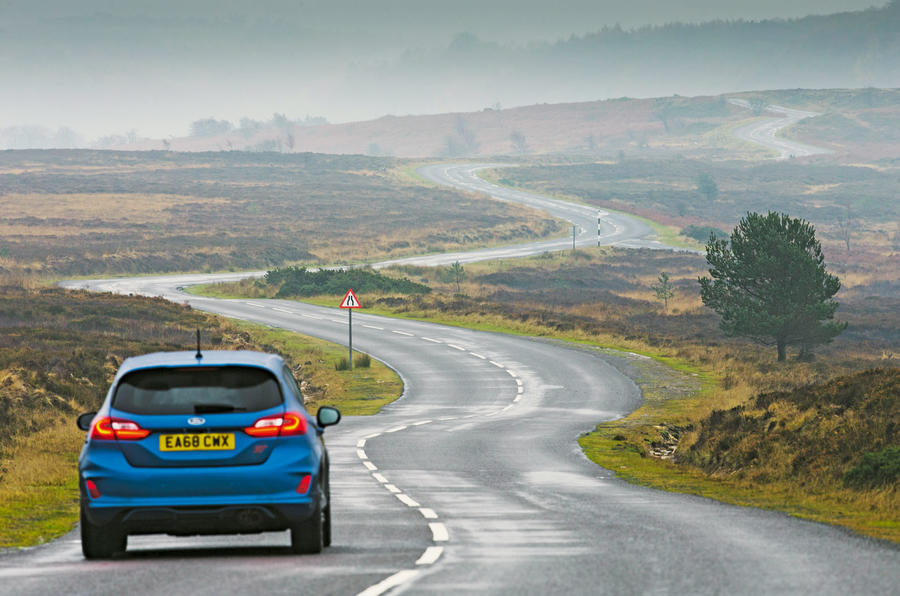
\includegraphics{car_driving}};
    \draw[red,thick] (-2.5, -2) rectangle (-0.75, -0.4);
  \end{tikzpicture}
  \caption{\footnotesize We could envision that in a sliding windows algorithm, the window with the maximal prediction for the object of interest may not even fully contain the car but instead only a portion of it due to the kernel size and stride length. Further, the best bounding box for the object may not be a square but instead rectangular in shape, and a sliding windows algorithm doesn't allow us to capture that.}
\end{figure}
One way to get more accurate bounding boxes is via the \href{https://arxiv.org/abs/1506.02640}{You Only Look Once} algorithm. Suppose we have an input image of dimension $100 \times 100$. We might overlay a coarser grid, say $19 \times 19$ over our original image such that we partition the original image into smaller cropped images. We will apply our image classification and localization algorithms learned previously to each of the cells in the partitioned grid. In particular, we need to learn how to create labels for such data: for each observation, i.e. each cell in each image, we create an eight dimensional vector $y = \begin{bmatrix} p_c & b_x & b_y & b_h & b_w & c_1 & c_2 & \ldots & c_k \end{bmatrix}$ where the first element describes whether there is an object in the (cropped) image, the next four elements describe the bounding box for the item associated with that grid cell, and the last items are the class probabilities. Suppose an image has two objects. When an object is found in an image (by hand, when creating the labels), we assign it to the cell which contains the midpoint of its bounding box; this ensures that each object is assigned to exactly one of the partitioning cells even if it spans multiple. So, for each grid cell in our partitioning, we end up with an eight-dimensional output vector. So if we used a $k \times k$ overlay,
we'll want our target output volume to be $k \times k \times 8$. So in our example, the input might be $100 \times 100 \times 3$, and our job will be to choose conv-layers and max-pool layers such that we eventually map to a $k \times k \times 8$ output volume. We then have input images and target labels, and we can use back propagation to train the neural network to learn to map from any input image $X$ to this type of output volume $Y$.

Notice that the algorithm should work okay contingent upon there not being more than a single object in each of the partitioning cells; using a finer grid helps to address this problem. Further, notice that the algorithm is a lot of like the image classification algorithm learned earlier in that we can output precise bounding boxes that are not subject to the stride size of sliding windows.

One point worth hashing out is how to define $b_x, b_y, b_h, b_w$. We can normalize each grid cell such that its upper left point is $(0,0)$ and the lower-right point is $(1,1)$. Then, $b_x, b_y$ specifiy the mid-points and are are guaranteed to lie within the unit interval by definition of assigning each object to the grid cell which contains its mid-point. The height and width $b_h, b_w$ are specified relative to the size of the partitioning cell, and so they theoretically could be larger than one. There are some further enhancements we can make, like for example applying a sigmoid function to $b_x,b_y$ to ensure they lie in the unit interval and applying an exponential function to $b_h, b_w$ to ensure they are non-negative.

\subsubsection{Intersection over Union} This is a technique that can help evaluate your object detection algorithm, and we'll later show how it can be added as a feature to a model to make it work even better. In the object detection task, you're expected to \emph{localize} the object after detecting it. Suppose we have an image with a ground-truth label in \color{purple}{purple}\color{black}, and our algorithm has output a bounding box in \color{orange}{orange}\color{black}: is this a good bounding box?

\begin{figure}[h]
  \centering
  \begin{tikzpicture}
    \node at (0, 0) {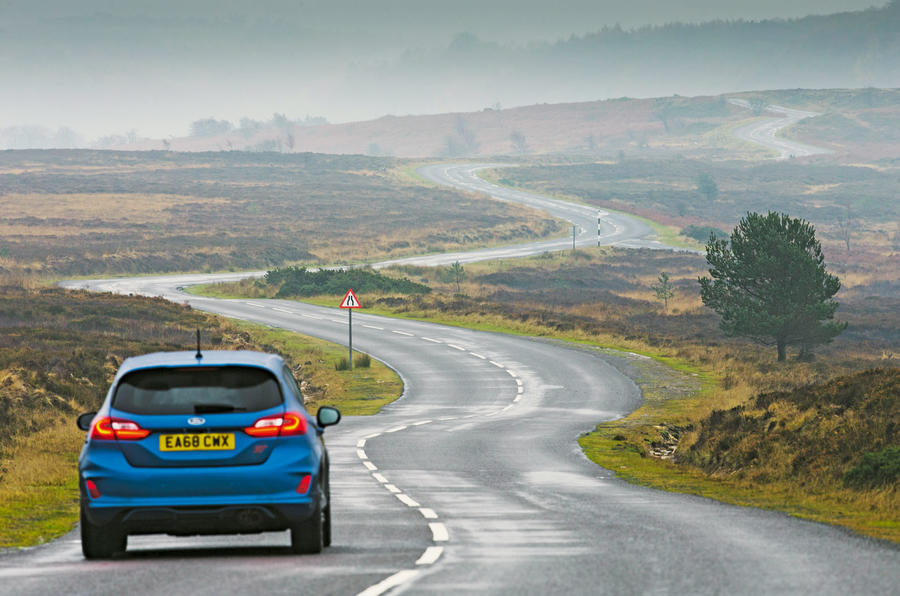
\includegraphics{car_driving}};
    \draw[purple,thick]    (-3.2, -2.2) rectangle (-0.8, -0.4);
    \draw[orange,thick] (-2.8, -2)   rectangle (-1.2, -0.2);
  \end{tikzpicture}
\end{figure}

The intersection-over-union computes the intersection over the union of the two bounding boxes. To be clear: the union is any area contained in either bounding box, whereas the intersection is the region that is contained in box bounding boxes. By dividing the size of the intersection by the size of the union, we can get a scalar value describing precision of the bounding box; by convention if Intersection Over Union (IOU) exceeds 1/2 then computer-vision researchers say the bounding box was correctly computed. In the event that the boxes overlap perfectly, IOU takes on unit value.

\subsubsection{Non-max suppression} One of the problems with object detection as we've learned so far is that an algorithm can find multiple detections of the same object: rather than detecting it just once it might detect it multiple times. Non-max suppression is a technique for ensuring that each object gets detected only once. The fundamental problem is that, even when using an algorithm like YOLO where each object is assigned to a single grid cell by virtue of where its midpoint falls, each of the neighboring cells may end up making a (mis)-prediction that the object's midpoint lies within it. Non-max suppression examines the $p_c$ alongside the largest $c_i$, and then compares this to the positive predictions with (high) IOU and suppress those predictions. This ensures that for each area of the image, we are taking the bounding box we are most confident in having detected an object within, and simultaneously ensures that we end up with a single bounding box per object. The non-max suppression names literally derives from the fact that we are going to output the maximal probabilities for classifications but suppress the close by ones that are non-maximal.

\paragraph{Implementing non-max suppression} To actually implement non-max suppression, we will carry it out once per class. So for the sake of this example, suppose there is only a single class and that $p_c$ contains the probability of an object residing in that partition of the image. start by discarding all predictions for bounding boxes with
max $p_c$ below some threshold (say 1/2): unless we think there's a reasonable chance of there being an object in that partition of the image, we'll just discard the prediction. Next, while there remain any bounding boxes yet to be processed: pick the bounding box with the highest probability of containing an object and commit to making that a prediction; the subsequent step will be to discard any remaining bounding boxes that have a high IOU with the bounding box we just committed to.
\begin{algorithm}
  \caption{Non-Max Suppression}
  Discard all boxes with $p_c \leq \texttt{threshold}$ \\
  \While{bounding boxes remain yet to be processed} {
    Pick the box with largest $p_c$, commit to that as a prediction. \\
    Discard any remaining box with IOU $\geq 1/2$ with the bounding box just     committed to.
  }
\end{algorithm}

At the conclusion of this algorithm, we'll have considered each bounding box and either output it as a prediction or discarded it due to having too large IOU with one of the bounding boxes already committed to.

\subsubsection{Anchor Boxes} One of the problems with object detection algorithms as learned so far is that each of the grid cells can only detect a single object. What if a grid cell contains multiple objects? To solve this problem, we use anchor boxes. Let's consider an example where there is a person standing in front of a car, and we've chosen to use a coarse grid such that the midpoint of the car and the midpoint of the person that we're trying to detect both land in the same central grid cell. As we've defined our output vector $y = \begin{bmatrix} p_c & b_x & b_y & b_h & b_w & c_1 & c_2 & \ldots & c_k \end{bmatrix}$ there is no way to encode the existence of multiple objects (let alone multiple bounding boxes. We might choose two differently shaped anchor boxes:
\begin{figure}[h]
  \centering
  \begin{tikzpicture}
    \draw (0,0) rectangle (1, 2) node[above left] {Anchor box 1};
    \draw (2,1) rectangle (4, 2) node[above left] {Anchor box 2};
  \end{tikzpicture}
  \caption{\footnotesize Two simple types of anchor boxes; perhaps the first is more suitable to bounding a standing person, versus the latter for a car depicted from its side profile.}
\end{figure}
Then, for each object detect in each cell, we'll assign it to the anchor box that matches its shape most closely (we can have several bounding boxes, say 5 to choose from). To be explicit, we still assign each object to the cell containing its midpoint, but we choose the anchor box which has the highest IOU for the object. Then, our label vector $y$ will have components
$p_c, b_x, b_y, b_h, b_w, c_1, c_2, \ldots, c_k$ for \emph{each} of the anchor boxes.
\begin{figure}[h]
  \centering
  \begin{tikzpicture}
    \node at (0,0) {y = };
    \draw (0.5, -3) rectangle (1, 3);
    \node at (0.75, 2.8) {$p_c$};
    \node at (0.75, 2.3) {$b_x$};
    \node at (0.75, 1.8) {$b_y$};
    \node at (0.75, 1.3) {$b_h$};
    \node at (0.75, 0.8) {$b_w$};
    \node at (0.75, 0.3) {$\vdots$};
    \node at (0.75, -.2) {$c_k$};
    \draw[decorate,decoration={brace,amplitude=10pt,mirror,raise=4pt},yshift=0pt]
(1.2,-0.2) -- (1.2,2.8) node [black,midway,xshift=1.25cm] {\footnotesize Anchor 1};
    \draw[decorate,decoration={brace,amplitude=10pt,mirror,raise=4pt},yshift=0pt]
(1.2,-3) -- (1.2,-0.25) node [black,midway,xshift=2cm] {\footnotesize Anchors $2, \ldots, k$};
  \end{tikzpicture}
  \caption{\footnotesize If we use $k$ anchor boxes, then for each grid cell in each labeled image in our training data, we will require knowledge of $p_c$, the bounding box descriptors, and the class probabilities. In addition to assigning each object to the cell which contains its midpoint, we assign an anchor box to it by comparing the ground-truth bounding box with each of the proposed anchor boxes and computing IOU: the anchor box with highest similarity (IOU) is chosen to describe that object. For anchor boxes that are not used within a cell, we can simply set their $p_c = 0$ to indicate there is no object being bounded by that anchor in that cell.}
\end{figure}
Cases that this algorithm does not handle well: what if we have more objects than exist anchor boxes within a single cell? Or, what if two objects in the same cell have the same anchor box shape? This algorithm doesn't deal with these cases well.

How do we choose anchor box sizes? We can use a $k$-means algorithm to partition the objects into different classes, and then select an anchor box that best fits the types of images that fall into each class. It's also possible to choose anchor boxes by hand as follows: simply choose boxes that reasonably can contain the objects your interested in detecting.

\subsubsection{YOLO Object Detection Algorithm}
Let's see how to put the components discusses above together to form a YOLO object detection algorithm.

\paragraph{Constructing a training set}
Let's first see how to construct a training data set. Suppose we are interested in classifying three types of objects: pedestrians, cars, and motorcycles. Suppose we are using two different anchor sizes, and that for illustration sake we have chosen to partition our input images into $3 \times 3$. Then each image is a volume that is $3 \times 3 \times 2 \times (5 + k)$, where the two comes from the number of anchor boxes used and the $(5 + k)$ comes from the fact that we require a $p_c, b_x, b_y b_h, b_w, c_1, c_2, \ldots, c_k$ to describe if an object is in a grid cell as well as to localize it. To construct the training set, we have to go through \emph{each} cell of \emph{each} image, and construct the appropriate target $y$ vector describing whether there's an object and where it is in the grid cell.

\paragraph{Training a conv-net} Our input images might be
$100 \times 100 \times 3$: our conv-net would take this and output the appropriate volume
$3 \times 3 \times 2 \times (5 + k)$ as described above. Given an image, your neural network will compute this volume describing for each cell whether there is an object (and if so localize it as well). For much of the parts of the image, the component $p_c$ of each anchor box will be zero, indicating that the remaining numbers describing the bounding box and class probabilities for that bounding box don't actually mean anything. Finally, we run our predictions through non-max suppression for \emph{each} of the classes we're interested in predicting, independently.

\paragraph{\href{https://arxiv.org/abs/1311.2524}{Region Proposals}} This is an influential body of work. Recall sliding windows which involves conceptually running a classifier across different croppings of the image. We can of course run the algorithm convolutionally, but it unfortunately spends a lot of compute on regions of the image that just don't contain any objects of interest. 
Rather than running your conv-net on all sliding windows, they propose only computing your conv-net on smaller subset(s) of the image. The way that region proposal is carried out is to run a \emph{segmentation} algorithm on the input image and then use this to decide where to run your classifier. For each region of interest returned by the segmentation algorithm, we run our conv-net for which we get a prediction for an object and also a bounding box. There's also
a convolutional implementation which allows for making predictions across all areas of interest returned from the segmentation algorithm, known as \href{https://arxiv.org/abs/1504.08083}{Fast R-CNN}. Then, there's \href{https://arxiv.org/abs/1506.01497}{Faster R-CNN} which uses a conv-net as the basis for the segmentation algorithm and this in turn runs even faster.

\subsection{Face Recognition} A special application of conv-nets is facial recognition and neural style transfer. Let's start with defining some terms used in the face recognition literature.
\begin{itemize}
  \item The face verification problem is as follows: you'ure given an input image as well as the name or ID of a person, and the job of the system is to verify whether the input image is that of the \emph{claimed} person.
\item In the recognition problem, we have a database of $K$ persons, and we are given an input image: we then wish to output the ID of the individual if one of the $K$ persons (or output ``not recognized'').
\end{itemize}
The recognition problem is much harder than the verification problem: suppose we have a verification system that only commits 1\% error, then when applied to a recognition system responsible for 100 people we're likely to make a mistake.

\paragraph{One shot learning} One of the problems of facial recognition is that it's a one-shot learning problem: that is, you need to be able to recognize a person given just a single image or one example of their face. Historically, deep learning algorithms don't perform well if you only have a single example.
As an example, suppse you have a database that consists of an employee-id photo for each employee in your company. Now, suppose somebody shows up at an automatic turnstyle and wants to be let in: the system has to recognize (i)
whether the person is contained in the database and (ii) which individual it is. One approach could be to attempt to use a conv-net; this approach won't work well since we need to retrain our classifier each time a new member joins our team. Instead, we learn a similarity function: $d(\texttt{image1}, \texttt{image2})$ where if the images are similar a small number is returned and if the images are very different a large number is returned. Then, at inference time we can simply compute $d$ given two images and compare against some fixed threshold. Notice that this allows us to solve the one-shot learning problem: if we add a new person to the team, there's no need to retrain a new function we can simply compare an arbitrary image to our new set.

\paragraph{Siamese Network} A good way to learn a similarity function is to use a Siamese network. We've seen before conv-net architectures that take an input image, map it through a sequence of transformations to some specified volume, then apply several fully connected layers before making a prediction using a softmax classifier.

\begin{figure}[h]
  \centering
  \begin{tikzpicture}
    \pgfmathsetmacro{\cubex}{2} 
    \pgfmathsetmacro{\cubey}{1} 
    \pgfmathsetmacro{\cubez}{1}
    \draw[black, fill=blue!60] (0,0,0) -- ++(-\cubex,0,0) -- ++(0,-\cubey*2,0) -- ++(\cubex,0,0) -- cycle; 
    \draw[black, fill=blue!60] (0,0,0) -- ++(0,0,-\cubez/2) -- ++(0,-\cubey*2,0) -- ++(0,0,\cubez/2) -- cycle; 
    \draw[black, fill=blue!60] (0,0,0) -- ++(-\cubex,0,0) -- ++(0,0,-\cubez/2)     -- ++(\cubex,0,0) -- cycle;
  \draw[->] (0.5, -0.75) -- (1.5, -0.75) {};
    \draw[black, fill=blue!60] (3,-0.5,0) -- ++(-\cubex*10/14,0,0) -- ++(0,-\cubey*2*10/14,0) -- ++(\cubex*10/14,0,0) -- cycle; 
    \draw[black, fill=blue!60] (3,-0.5,0) -- ++(0,0,-\cubez) -- ++(0,-\cubey*2*10/14,0) -- ++(0,0,\cubez) -- cycle; 
    \draw[black, fill=blue!60] (3,-0.5,0) -- ++(-\cubex*10/14,0,0) -- ++(0,0,-\cubez)     -- ++(\cubex*10/14,0,0) -- cycle;
  \draw[->] (3.75, -0.75) -- (5, -0.75) {};
    \draw[black, fill=blue!60] (6,-1,0) -- ++(-\cubex*5/14,0,0) -- ++(0,-\cubey*2*5/14,0) -- ++(\cubex*5/14,0,0) -- cycle; 
    \draw[black, fill=blue!60] (6,-1,0) -- ++(0,0,-\cubez) -- ++(0,-\cubey*2*5/14,0) -- ++(0,0,\cubez) -- cycle; 
    \draw[black, fill=blue!60] (6,-1,0) -- ++(-\cubex*5/14,0,0) -- ++(0,0,-\cubez)     -- ++(\cubex*5/14,0,0) -- cycle;
  \draw[->] (6.75, -0.75) -- (7.25, -0.75) node[above left] {\footnotesize FC};
  \draw[black] (7.5, -2) rectangle (8, 0.5);
  \node[draw,circle] at (7.75, 0.25) {};
  \node[draw,circle] at (7.75,-0.25) {};
  \node at (7.75,-0.75) {$\vdots$};
  \node[draw,circle] at (7.75,-1.75) {};
  \draw[->] (8.25, -0.75) -- (9, -0.75) node[above left] {\footnotesize FC};
  \draw[black] (9.5, -2) rectangle (10, 0.5);
  \node[draw,circle] at (9.75, 0.25) {};
  \node[draw,circle] at (9.75,-0.25) {};
  \node at (9.75,-0.75) {$\vdots$};
  \node[draw,circle] at (9.75,-1.75) {};
  \draw[->] (10.25, -0.75) -- (10.75, -0.75);
  \node[draw,circle] at (11, -0.75) {};
  \node at (11, -1.25) {$\substack{y \\ \textrm{softmax}}$};
  \end{tikzpicture}
  \caption{\footnotesize A prototypical conv-net architecture, applying filters and pooling to end up with a volume that is then fed into fully connected layers. In this part of the lecture notes, we're going to focus on the set of features derived from the last hidden layer.}
\end{figure}
We can think of the mapping from an input image to the set of neurons in the last hidden layer of the conv-net above as an \emph{encoding} of the image:
given an image we represent it using however many hidden neurons are in this last layer through a learned function $f$. Then, given two input images we feed them each through the neural network to obtain two separate encodings (real-valued vectors): we can then define a distance function $d$ to be the normed difference between the two encodings.
$$
d(x_1, x_2) = \| f(x_1) - f(x_2)\|_2^2
$$
This idea is inspired by \href{https://research.fb.com/publications/deepface-closing-the-gap-to-human-level-performance-in-face-verification/}{DeepFace}.
More formally, the parameters of the network define an encoding $f$ of an input image. We'd like to train a network and learn parameters such that if two pictures $x_i$ and $x_j$ are of the same person, then the difference between their encodings should be small; correspondingly if $x_i$ and $x_j$ are pictures of different people, we'd like the difference between their encodings to be very large. Let's next learn a loss function that allows us to cary out this objective.

\subsubsection{\href{https://arxiv.org/abs/1503.03832}{Triplet Loss}} One way to ensure that we learn a good encoding for your pictures is to define and apply gradient descent on the triplet loss function. To apply triplet loss, you need to compare \emph{pairs} of images. In the terminology of triplet loss, you're always going to look at an \emph{anchor} image and whenever you compare it to a \emph{positive} example (e.g. the same person) you want the distance to be small. Whereas, when the anchor is compared to a \emph{negative} example you'ld like the distance to be much further apart. The term triplet loss comes from the fact that we'll always consider triplets of images: an anchor image $A$, a positive image $P$, and a negative image $N$. We want
\[
\underbrace{\|f(A) - f(P)\|^2}_{d(A,P)} \leq \underbrace{\|f(A) - f(N)\|^2}_{d(A,N)} \implies \|f(A) - f(P)\|^2 - \|f(A) - f(N)\|^2 \leq 0
\]
Realize that a network could learn to output zeros for any image and then this equation would be satisfied: in this case $f(\cdot) = 0$ and everything becomes zero and the inequality is satisfied with equality. Equivalently, if the network learned the \emph{same} encoding for \emph{every} image then this inequality would also be satisfied. To prevent the neural network from doing either of these two things, we'll modify our objective function to require that
\[
\|f(A) - f(P)\|^2 - \|f(A) - f(N)\|^2 \leq -\alpha
\]
where now $\alpha$ is some hyperparameter that prevents the network from outputting trivial encodings. A more standard way to write the above expression is 
\[
\|f(A) - f(P)\|^2 - \|f(A) - f(N)\|^2 + \alpha \leq 0
\]
where now we can call $\alpha$ the \emph{margin}. Now, given our three images anchor $A$, positive $P$, and negative $N$, we define our loss function
\[
\mathcal L (A, P, N) = \max{\{\|f(A) - f(P)\|^2 - \|f(A) - f(N)\|^2 + \alpha, 0\}}
\]
By applying gradient descent to try and minimize this, this has the effect of sending the first argument to be less than or equal to zero as desired. The overall cost function can be summed over a training set consisting of different triplets.
\[
J = \sum_{i=1}^m \mathcal L(A^{(i)}, P^{(i)}, N^{(i)})
\]
To make this clear, suppose you have a training set of 10k pictures with 1k different persons. You'd have to use these 10k images to manually create triplets with a positive and negative image associated to each anchor. Notice that in order to create a triplet, we do need $A$ and $P$ to be the same person, so you require a training dataset where each person appears multiple times.

\paragraph{Choosing triplets $A$, $P$, $N$} If we constrain $A$ and $P$ to be images containing the same person but choose $N$ randomly, then it will be quite easy for our network to learn to satisfy $d(A,P) + \alpha \leq d(A,N)$ since if $A$ and $N$ are two randomly chosen persons there is a good chance their distance will exceed the margin; so, the neural network won't learn much from such an example. What we'd like to do is to train on triplets that are ``hard'', where $d(A,P) \approx d(A,N)$: in this case the network has to learn to push the former downward or the latter upward. The paper \href{https://arxiv.org/abs/1503.03832}{FaceNet} has details on how to choose triplets wisely to speed up training.

\paragraph{Face verification and binary classification} Triplet loss is one good way to learn the parameters of a conv-net for face recognition. There's another way to learn these parameters: by posing face recognition as a binary classification problem. We can train a neural network, have it output an embedding, and then input these for both images into a logistic regression unit to make a prediction; the target label will be unit valued if the images are of the same person and zero otherwise.

\begin{figure}[h]
  \centering
  \begin{tikzpicture}
    \pgfmathsetmacro{\cubex}{2} 
    \pgfmathsetmacro{\cubey}{1} 
    \pgfmathsetmacro{\cubez}{1}
    \draw[black, fill=blue!60] (0,0,0) -- ++(-\cubex,0,0) -- ++(0,-\cubey*2,0) -- ++(\cubex,0,0) -- cycle; 
    \draw[black, fill=blue!60] (0,0,0) -- ++(0,0,-\cubez/2) -- ++(0,-\cubey*2,0) -- ++(0,0,\cubez/2) -- cycle; 
    \draw[black, fill=blue!60] (0,0,0) -- ++(-\cubex,0,0) -- ++(0,0,-\cubez/2)     -- ++(\cubex,0,0) -- cycle;
  \draw[->] (0.5, -0.75) -- (1.5, -0.75) {};
    \draw[black, fill=blue!60] (3,-0.5,0) -- ++(-\cubex*10/14,0,0) -- ++(0,-\cubey*2*10/14,0) -- ++(\cubex*10/14,0,0) -- cycle; 
    \draw[black, fill=blue!60] (3,-0.5,0) -- ++(0,0,-\cubez) -- ++(0,-\cubey*2*10/14,0) -- ++(0,0,\cubez) -- cycle; 
    \draw[black, fill=blue!60] (3,-0.5,0) -- ++(-\cubex*10/14,0,0) -- ++(0,0,-\cubez)     -- ++(\cubex*10/14,0,0) -- cycle;
  \draw[->] (3.75, -0.75) -- (5, -0.75) {};
    \draw[black, fill=blue!60] (6,-1,0) -- ++(-\cubex*5/14,0,0) -- ++(0,-\cubey*2*5/14,0) -- ++(\cubex*5/14,0,0) -- cycle; 
    \draw[black, fill=blue!60] (6,-1,0) -- ++(0,0,-\cubez) -- ++(0,-\cubey*2*5/14,0) -- ++(0,0,\cubez) -- cycle; 
    \draw[black, fill=blue!60] (6,-1,0) -- ++(-\cubex*5/14,0,0) -- ++(0,0,-\cubez)     -- ++(\cubex*5/14,0,0) -- cycle;
  \draw[->] (6.75, -0.75) -- (7.25, -0.75) node[above left] {\footnotesize FC};
  \draw[black] (7.5, -2) rectangle (8, 0.5);
  \node[draw,circle] at (7.75, 0.25) {};
  \node[draw,circle] at (7.75,-0.25) {};
  \node at (7.75,-0.75) {$\vdots$};
  \node[draw,circle] at (7.75,-1.75) {};
  \draw[->] (8.25, -0.75) -- (9, -0.75) node[above left] {\footnotesize FC};
  \draw[black] (9.5, -2) rectangle (10, 0.5);
  \node[draw,circle] at (9.75, 0.25) {};
  \node[draw,circle] at (9.75,-0.25) {};
  \node at (9.75,-0.75) {$\vdots$};
  \node[draw,circle] at (9.75,-1.75) {};
  %% Second layer
  \draw[black, fill=blue!60] (0,-3,0) -- ++(-\cubex,0,0) -- ++(0,-\cubey*2,0) -- ++(\cubex,0,0) -- cycle; 
  \draw[black, fill=blue!60] (0,-3,0) -- ++(0,0,-\cubez/2) -- ++(0,-\cubey*2,0) -- ++(0,0,\cubez/2) -- cycle; 
    \draw[black, fill=blue!60] (0,-3,0) -- ++(-\cubex,0,0) -- ++(0,0,-\cubez/2)     -- ++(\cubex,0,0) -- cycle;
  \draw[->] (0.5, -3.75) -- (1.5, -3.75) {};
    \draw[black, fill=blue!60] (3,-3.5,0) -- ++(-\cubex*10/14,0,0) -- ++(0,-\cubey*2*10/14,0) -- ++(\cubex*10/14,0,0) -- cycle; 
    \draw[black, fill=blue!60] (3,-3.5,0) -- ++(0,0,-\cubez) -- ++(0,-\cubey*2*10/14,0) -- ++(0,0,\cubez) -- cycle; 
    \draw[black, fill=blue!60] (3,-3.5,0) -- ++(-\cubex*10/14,0,0) -- ++(0,0,-\cubez)     -- ++(\cubex*10/14,0,0) -- cycle;
  \draw[->] (3.75, -3.75) -- (5, -3.75) {};
    \draw[black, fill=blue!60] (6,-4,0) -- ++(-\cubex*5/14,0,0) -- ++(0,-\cubey*2*5/14,0) -- ++(\cubex*5/14,0,0) -- cycle; 
    \draw[black, fill=blue!60] (6,-4,0) -- ++(0,0,-\cubez) -- ++(0,-\cubey*2*5/14,0) -- ++(0,0,\cubez) -- cycle; 
    \draw[black, fill=blue!60] (6,-4,0) -- ++(-\cubex*5/14,0,0) -- ++(0,0,-\cubez)     -- ++(\cubex*5/14,0,0) -- cycle;
  \draw[->] (6.75, -3.75) -- (7.25, -3.75) node[above left] {\footnotesize FC};
  \draw[black] (7.5, -5) rectangle (8, -2.5);
  \node[draw,circle] at (7.75, -2.75) {};
  \node[draw,circle] at (7.75,-3.25) {};
  \node at (7.75,-3.75) {$\vdots$};
  \node[draw,circle] at (7.75,-4.75) {};
  \draw[->] (8.25, -3.75) -- (9, -3.75) node[above left] {\footnotesize FC};
  \draw[black] (9.5, -5) rectangle (10, -2.5);
  \node[draw,circle] at (9.75, -2.75) {};
  \node[draw,circle] at (9.75,-3.25) {};
  \node at (9.75,-3.75) {$\vdots$};
  \node[draw,circle] at (9.75,-4.75) {};
  \draw[->] (10.25, -0.75) -- (11, -2);
  \draw[->] (10.25, -3.75) -- (11, -2);
  \node[draw,circle] at (11.25, -2) {};
  \draw[->] (11.5, -2) -- (12, -2);
  \node at (12.25, -2) {$\hat y$};
  \end{tikzpicture}
  \caption{\footnotesize We could take a pair of neural networks, i.e. a Siamese network, and have them both compute embeddings for each image. We then feed these embeddings (or perhaps their difference) as input into a logistic regression unit to make a prediction. The two neural networks are called \emph{siamese} because they share the same parameters. The training dataset will now consist of \emph{pairs} of images, where the label is unit valued if the images contain the same person and zero otherwise.}
\end{figure}
What is our logistic regression unit really doing? Well, if we feed it as input the difference between the two encodings returned by our images fed into our network,
\[
\hat y = \sigma \left( \sum_{k=1}^{\textrm{length of encoding}} w_k |f(x^{(i)})_k - f(x^{(j)})_k| + b\right)
\]
and the job of the logistic regression unit would be to learn weights $w_k$'s and $b$ such that our logistic loss is minimized.
Instead of taking a simple difference between our two encodings, we could also consider a $\chi^2$ similarity:
\[
\frac{\left(f(x^{(i)})_k - f(x^{(j)})_k\right)^2}{f(x^{(i)})_k + f(x^{(j)})_k}
\]

\paragraph{Precomputing embeddings for each employee in our database}
As an implementation detail: if we are deploying a system we may wish to precompute the encodings for each employee in our database, that way when a new employee walks through the turnstyle hoping to be recognized we can just run their image through the upper layer of the siamese network and compare it to the pre-computed embeddings for each known employee in the database.

\subsection{\href{https://arxiv.org/abs/1508.06576}{Neural Style Transfer}} The idea of neural style transfer is to take some raw image \emph{content} $c$ and compose a new generated image $g$ using some style $s$. In order to implement neural style transfer, we'll have to inspect the features at various hidden layers of a conv-net.
\paragraph{What are deep conv-nets learning?} What are the deeper layers of a conv-net really learning? Suppose we've trained an AlexNet network.
\begin{figure}[h]
  \begin{tikzpicture}
    \pgfmathsetmacro{\cubex}{2} 
    \pgfmathsetmacro{\cubey}{1} 
    \pgfmathsetmacro{\cubez}{1}
    \node at (-2, 0) {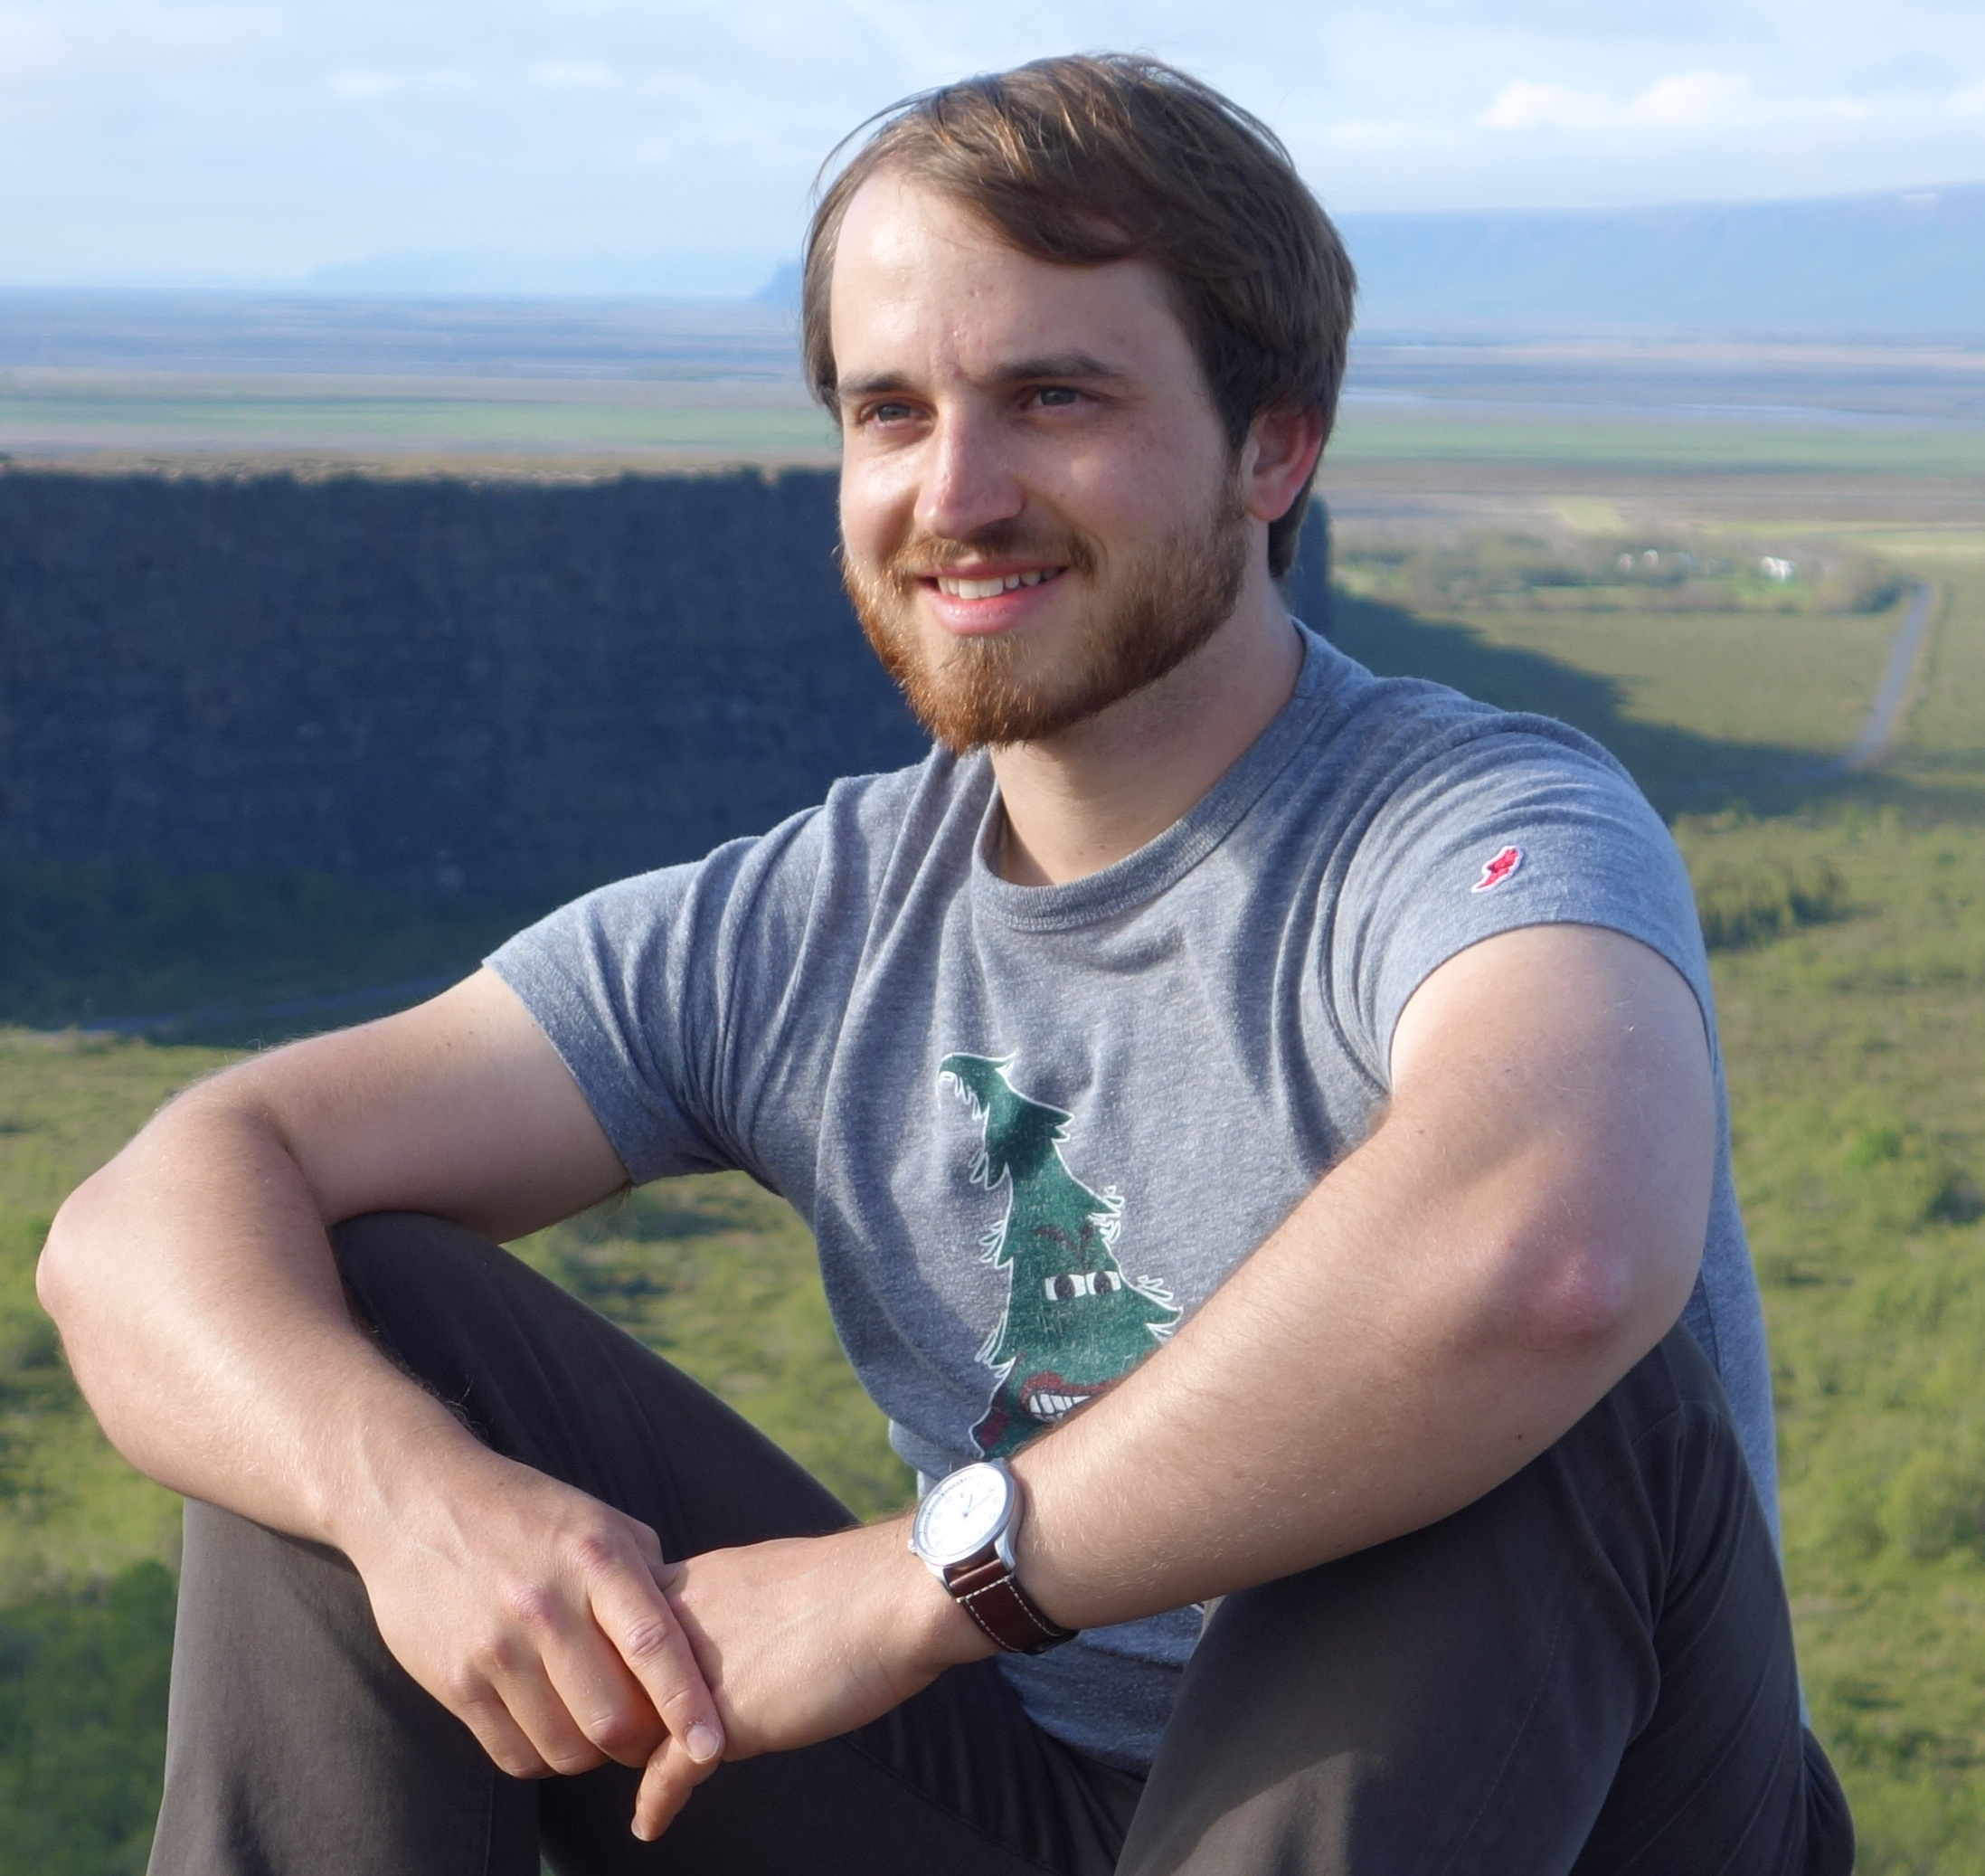
\includegraphics[scale=0.15]{profile}};
    \node at (-2,-1.35) {$\scriptstyle 224 \times 224 \times 3$};
    \draw[black, fill=blue!60] (1.75,0.5,0) -- ++(-\cubex,0,0) -- ++(0,-\cubey*2,0) -- ++(\cubex,0,0) -- cycle; 
    \draw[black, fill=blue!60] (1.75,0.5,0) -- ++(0,0,-\cubez*2) -- ++(0,-\cubey*2,0) -- ++(0,0,\cubez*2) -- cycle; 
    \draw[black, fill=blue!60] (1.75,0.5,0) -- ++(-\cubex,0,0) -- ++(0,0,-\cubez*2)     -- ++(\cubex,0,0) -- cycle;
  \node at (1, -1.75) {$\scriptstyle 110 \times 110 \times 96$};
    \draw[black, fill=blue!60] (4.5,0.5,0) -- ++(-\cubex*10/14,0,0) -- ++(0,-\cubey*2*10/14,0) -- ++(\cubex*10/14,0,0) -- cycle; 
    \draw[black, fill=blue!60] (4.5,0.5,0) -- ++(0,0,-\cubez) -- ++(0,-\cubey*2*10/14,0) -- ++(0,0,\cubez) -- cycle; 
    \draw[black, fill=blue!60] (4.5,0.5,0) -- ++(-\cubex*10/14,0,0) -- ++(0,0,-\cubez)     -- ++(\cubex*10/14,0,0) -- cycle;
  \node at (4, -1.25) {$\scriptstyle 55 \times 55 \times 96$};
    \draw[black, fill=blue!60] (6,0.25,0) -- ++(-\cubex*5/14,0,0) -- ++(0,-\cubey*2*5/14,0) -- ++(\cubex*5/14,0,0) -- cycle; 
    \draw[black, fill=blue!60] (6,0.25,0) -- ++(0,0,-\cubez*1.5) -- ++(0,-\cubey*2*5/14,0) -- ++(0,0,\cubez*1.5) -- cycle; 
    \draw[black, fill=blue!60] (6,0.25,0) -- ++(-\cubex*5/14,0,0) -- ++(0,0,-\cubez*1.5)     -- ++(\cubex*5/14,0,0) -- cycle;
\node at (6, -1) {$\scriptstyle 26 \times 26 \times 256$};
    \draw[black, fill=blue!60] (7.5,0,0) -- ++(-\cubex*2/10,0,0) -- ++(0,-\cubey*2*2/10,0) -- ++(\cubex*2/10,0,0) -- cycle; 
    \draw[black, fill=blue!60] (7.5,0,0) -- ++(0,0,-\cubez*2) -- ++(0,-\cubey*2*2/10,0) -- ++(0,0,\cubez*2) -- cycle; 
    \draw[black, fill=blue!60] (7.5,0,0) -- ++(-\cubex*2/10,0,0) -- ++(0,0,-\cubez*2)     -- ++(\cubex*2/10,0,0) -- cycle;
    \node at (7.75, -1) {$\scriptstyle 13 \times 13 \times 256$};
    \draw[black, fill=blue!60] (9,0,0) -- ++(-\cubex*2/10,0,0) -- ++(0,-\cubey*2*2/10,0) -- ++(\cubex*2/10,0,0) -- cycle; 
    \draw[black, fill=blue!60] (9,0,0) -- ++(0,0,-\cubez*3) -- ++(0,-\cubey*2*2/10,0) -- ++(0,0,\cubez*3) -- cycle; 
    \draw[black, fill=blue!60] (9,0,0) -- ++(-\cubex*2/10,0,0) -- ++(0,0,-\cubez*3)     -- ++(\cubex*2/10,0,0) -- cycle;
    \node at (9.5, -1) {$\scriptstyle 13 \times 13 \times 384$};
    \draw[black, fill=blue!60] (11,0,0) -- ++(-\cubex*2/10,0,0) -- ++(0,-\cubey*2*2/10,0) -- ++(\cubex*2/10,0,0) -- cycle; 
    \draw[black, fill=blue!60] (11,0,0) -- ++(0,0,-\cubez*3) -- ++(0,-\cubey*2*2/10,0) -- ++(0,0,\cubez*3) -- cycle; 
    \draw[black, fill=blue!60] (11,0,0) -- ++(-\cubex*2/10,0,0) -- ++(0,0,-\cubez*3)     -- ++(\cubex*2/10,0,0) -- cycle;
    \node at (11.25, -1) {$\scriptstyle 13 \times 13 \times 384$};
    \draw[black, fill=blue!60] (13,0,0) -- ++(-\cubex*2/14,0,0) -- ++(0,-\cubey*2*2/14,0) -- ++(\cubex*2/14,0,0) -- cycle; 
    \draw[black, fill=blue!60] (13,0,0) -- ++(0,0,-\cubez) -- ++(0,-\cubey*2*2/14,0) -- ++(0,0,\cubez) -- cycle; 
    \draw[black, fill=blue!60] (13,0,0) -- ++(-\cubex*2/14,0,0) -- ++(0,0,-\cubez)     -- ++(\cubex*2/14,0,0) -- cycle;
\node at (13.25, -1) {$\scriptstyle 6 \times 6 \times 256$};
\draw (14, -1) rectangle (14.5, 1);
\node[draw,circle,scale=0.75] at (14.25, 0.8) {};
\node[draw,circle,scale=0.75] at (14.25, 0.35) {};
\node at (14.25, 0) {$\vdots$};
\node[draw,circle,scale=0.75] at (14.25, -0.7) {};
\node at (14.25, -1.25) {$\scriptstyle 4096$};
\draw (15, -1) rectangle (15.5, 1);
\node[draw,circle,scale=0.75] at (15.25, 0.8) {};
\node[draw,circle,scale=0.75] at (15.25, 0.35) {};
\node at (15.25, 0) {$\vdots$};
\node[draw,circle,scale=0.75] at (15.25, -0.7) {};
\node at (15.25, -1.25) {$\scriptstyle 4096$};
\node at (16, 0) {$\hat y$};
\end{tikzpicture}
\end{figure}
Here's how we can visualize what the deeper layers are learning. Start with a hidden unit in layer 1: scan through your training set and find out which examples (or even what image patches) maximize that hidden units activation function. Notice that for a hidden unit in the first layer of our conv-net, it sees only a relatively small portion of the neural network, and correspondingly it makes sense to plot just a small image patch. So, for a given hidden unit, you might find the nine image patches that maximize that unit's activation. We can then repeat this process for different hidden units, each time figuring out what parts of our training dataset maximize each hidden unit's activation.
When we carry this process out, we might learn that hidden units in the first layer often learn to recognize simple features: such as edges (oriented in various ways) or a particular shade of color.

What if we repeat this same process at deeper hidden layers; realize first that each hidden unit in later hidden layers sees a larger region of the image. Later layers will detect more complex shapes and patterns. As we progress deeper into the network, a hidden unit might be responsible for detecting objects like cars or people, or landmark features like water.

\paragraph{Cost function for Generated images} How can we provide content image $c$ and a style image $s$ and instruct a neural network to provide a generated image $g$? We define a cost function that measures how good a generated image is. How do we define the quality of a generated image? Let's split our cost function into two parts.
\[
J(G) = \alpha J_{\texttt{content}}(C,G) + \beta J_{\texttt{style}}(S,G).
\]
The first part of the loss function measures the discrepancy in content between the generated image and the content image, whereas the latter term measures the discrepancy betewen the generated image with the proposed style. To generate a new image, we follow an algorithm.
\begin{algorithm}
  \caption{Neural style transfer}
  Initiliaze $G$ randomly, e.g. $G \in 100 \times 100 \times 3$ \\
  Use gradient descent to minimize our loss $J(G)$:, $G := G - \frac{\textrm{d}}{\textrm{d} G} J(G)$ where we update our pixels one at a time.
\end{algorithm}
\paragraph{Content cost function} Suppose we use a hidden layer $\ell$ to compute content cost. If $\ell$ is a small number, e.g. hidden layer one, it will force your generated image to create pixel values very similar to your content image. Whereas if you use a deeper layer, we are requesting similarities at higher levels of abstraction, e.g. ``if the content image has a dog, ensure the generated image does as well''. In practice, we'll want to choose an intermediary layer that is not too shallow or too deep.
\begin{itemize}
\item Suppose you use hidden layer $\ell$ to compute content cost.
\item Use a pre-trained conv-net (e.g. VGG network).
\item Let $a^{[\ell](C)}$ and $a^{[\ell](G)}$ be the activation of layer $\ell$   on the content and generated images respectively; if the two activations are similar, both images have similar content.
\item Define $J_{\texttt{content}}(C,G) = \frac{1}{2} \|a^{[\ell](C)} - a^{[\ell](G)}\|^2$
\end{itemize}
\paragraph{Style cost function} What does the style of an image mean?
\begin{figure}[h]
  \centering
  \begin{tikzpicture}
    \pgfmathsetmacro{\cubex}{2} 
    \pgfmathsetmacro{\cubey}{1} 
    \pgfmathsetmacro{\cubez}{1}
    \draw[ultra thick, draw = black, fill = blue , scale = 1/2] (-5.5, 0.5) grid (-1.5, 4.5) rectangle (-5.5, 0.5);     
    \draw[ultra thick, draw = black, fill = green, scale = 1/2] (-5.25, 0.25) grid (-1.25, 4.25) rectangle (-5.25, 0.25);     
    \draw[ultra thick, draw = black, fill = red, scale = 1/2] (-5, 0) grid (-1,     4) rectangle (-5, 0);
\draw[->] (-0.25, 1) -- (0.25, 1);
%% First volume
    \draw[black, fill=blue!60] (2.5,1.5,0) -- ++(-\cubex,0,0) -- ++(0,-\cubey*2,0) -- ++(\cubex,0,0) -- cycle; 
    \draw[black, fill=blue!60] (2.5,1.5,0) -- ++(0,0,-\cubez*2) -- ++(0,-\cubey*2,0) -- ++(0,0,\cubez*2) -- cycle; 
    \draw[black, fill=blue!60] (2.5,1.5,0) -- ++(-\cubex,0,0) -- ++(0,0,-\cubez*2)         -- ++(\cubex,0,0) -- cycle;
%% Second volume
    \draw[black, fill=blue!60] (5.5,1.5,0) -- ++(-\cubex*10/14,0,0) -- ++(0,-\cubey*2*10/14,0) -- ++(\cubex*10/14,0,0) -- cycle; 
    \draw[black, fill=blue!60] (5.5,1.5,0) -- ++(0,0,-\cubez) -- ++(0,-\cubey*2*10/14,0) -- ++(0,0,\cubez) -- cycle; 
    \draw[black, fill=blue!60] (5.5,1.5,0) -- ++(-\cubex*10/14,0,0) -- ++(0,0,-\cubez)     -- ++(\cubex*10/14,0,0) -- cycle;
\draw[->] (3.5, 1) -- (4, 1);
    %% Third volume
    \draw[black, fill=blue!60] (7.5,1,0) -- ++(-\cubex*5/14,0,0) -- ++(0,-\cubey*2*5/14,0) -- ++(\cubex*5/14,0,0) -- cycle; 
    \draw[black, fill=blue!60] (7.5,1,0) -- ++(0,0,-\cubez*1.5) -- ++(0,-\cubey*2*5/14,0) -- ++(0,0,\cubez*1.5) -- cycle; 
    \draw[black, fill=blue!60] (7.5,1,0) -- ++(-\cubex*5/14,0,0) --     ++(0,0,-\cubez*1.5)     -- ++(\cubex*5/14,0,0) -- cycle;
\draw[->] (6, 1) -- (6.5, 1);
    %% Long skinny volume
    \draw[black, fill=blue!60] (9,0.5,0) -- ++(-\cubex*2/10,0,0) -- ++(0,-\cubey*2*2/10,0) -- ++(\cubex*2/10,0,0) -- cycle; 
    \draw[black, fill=blue!60] (9,0.5,0) -- ++(0,0,-\cubez*2) -- ++(0,-\cubey*2*2/10,0) -- ++(0,0,\cubez*2) -- cycle; 
    \draw[black, fill=blue!60] (9,0.5,0) -- ++(-\cubex*2/10,0,0) --     ++(0,0,-\cubez*2)     -- ++(\cubex*2/10,0,0) -- cycle;
    \draw[->] (8.25, 1) -- (8.75, 1);
    \draw (10.5, 0) rectangle (11, 2);
\node[draw,circle,scale=0.75] at (10.75, 1.8) {};
\node[draw,circle,scale=0.75] at (10.75, 1.35) {};
\node at (10.75, 1) {$\vdots$};
\node[draw,circle,scale=0.75] at (10.75, 0.3) {};
\draw[->] (10, 1) -- (10.4, 1);
\draw[->] (11, 1) -- (11.35, 1);
\node at (11.65,1) {$\hat y$};
  \end{tikzpicture}
  \caption{\footnotesize Suppose we have an input image. We're used to seeing conv-net architectures in the style depicted above. Suppose you've chosen some layer $\ell$ to define a measure of style within an image. We will define style as the correlation between activations across different channels in this layer $\ell$ activation.}
\end{figure}
Let's suppose for concreteness that we have chosen a particular layer and it corresponds to some volume.
\begin{figure}[h]
  \centering
  \begin{tikzpicture}
    \pgfmathsetmacro{\cubex}{2} 
    \pgfmathsetmacro{\cubey}{1} 
    \pgfmathsetmacro{\cubez}{1}
    \draw[black, fill=blue!60] (2.5,1.5,0) -- ++(-\cubex,0,0) -- ++(0,-\cubey*2,0) -- ++(\cubex,0,0) -- cycle; 
    \draw[black, fill=blue!60] (2.5,1.5,0) -- ++(0,0,-\cubez*2) -- ++(0,-\cubey*2,0) -- ++(0,0,\cubez*2) -- cycle; 
    \draw[black, fill=blue!60] (2.5,1.5,0) -- ++(-\cubex,0,0) --     ++(0,0,-\cubez*2)         -- ++(\cubex,0,0) -- cycle;
\node at (0.25, 0.75) {$n_h$};
\node at (1.75, -0.75) {$n_w$};
\node at (3.5, -0.25) {$n_c$};
  \end{tikzpicture}
  \caption{\footnotesize We have fixed attention to layer $\ell$ in our conv-net depicted above, and we will focus on computing correlation between activations across different channels in this layer.}
\end{figure}
If our volume is $n_h \times n_w times n_c$, where for simplicity of illustration let us take $n_c = 5$ but in practice we would have many more channels. To capture style, examine channels pairwise and consider how correlated the activations are, for each of the $n_h \times n_w$ matrices of real numbered activations. Why does this capture style? Correlations tell us which of the high-level texture components (e.g. a vertical texture, or a shade of a particular color) tend to occur or not together in part of an image.
\begin{algorithm}
  \caption{Style Matrix}
  Let $a^{[\ell]}_{i,j,k}$ denote activation at layer $\ell$ in position $i,j,k$     of the volume (height, width, and channels respectively). \\
  $G^{[\ell]}$ will be a square $n_c^{[\ell]} \times n_c^{[\ell]}$ matrix which measures ``correlations''; in particular for a particular entry of our style matrix we can compute it as follows $G_{k,k'}^{[\ell]} = \sum_i^{n_h^{[\ell]}} \sum_j^{n_w^{[\ell]}} a^{[\ell]}_{ijk} a^{[\ell]}_{ijk'}$
\end{algorithm}
What we're technically computing is the un-normalized cross covariance, not a proper correlation. We compute this style-matrix for \emph{both} the generated image \emph{and} the style image. We then
\begin{align*}
  G_{k,k'}^{[\ell](S)} = \sum_i^{n_h^{[\ell]}} \sum_j^{n_w^{[\ell]}}   a^{[\ell](S)}_{ijk} a^{[\ell](S)}_{ijk'}, \hspace{25pt}
  G_{k,k'}^{[\ell](G)} = \sum_i^{n_h^{[\ell]}} \sum_j^{n_w^{[\ell]}} a^{[\ell](G)}_{ijk} a^{[\ell](G)}_{ijk'}
\end{align*}
Then, we define the style cost function as
\[
J_{\texttt{style}}^{[\ell]}(S,G) = \frac{1}{2 n_h^{[\ell]} n_w^{[\ell]} n_c^{[\ell]}}\|G^{[\ell](S)} - G^{[\ell](G)}\|_F^2 = \frac{1}{2 n_h^{[\ell]} n_w^{[\ell]} n_c^{[\ell]}} \sum_k \sum_{k'} \left(G^{[\ell](S)}_{kk'} - G^{[\ell](G)}_{kk'}\right)^2
\]
It turns out that we get more aesthetically pleasing images if we use the style cost function from multiple different layers. We can use additional hyperparameters to control weighting:
\begin{align*}
  J_{\texttt{style}}(S,G) = \sum_{\ell} \lambda^{[\ell]} J_{\texttt{style}}^{[\ell]}(S,G)
\end{align*}
This allows us to use multiple layers, including earlier ones which capture stylistic similarities at a low level, as well as later layers which capture stylistic similarities at a higher level of abstraction.

\subsubsection{1D and 3D Generalizations} Most of our discussion has focused on 2D input data. Many of the techniques we've learned about also extend to 1 and 3D data. We've already seen how 2D convolutions work:
\begin{figure}[h]
  \centering
  \begin{tikzpicture}
    \draw[step=0.1] (0,0) grid (1.4, 1.4);
    \node at (0.5, -0.25) {\footnotesize 2D input image};
    \node at (0.5, -0.5)  {$\scriptstyle 14 \times 14$};
    \node at (1.8, 0.7) {*};
    \draw[step=0.1] (2.2, 0.4) grid (2.7, 0.9);
    \node at (2.5, 0.25) {\footnotesize 2D filter};
    \node at (2.5, 0) {$\scriptstyle 5 \times 5$};
    \node at (3, 0.7) {=};
    \draw[step=0.1] (3.4, 0) grid (4.4, 1);
    \node at (3.9, -0.2) {$\scriptstyle 10 \times 10$};
  \end{tikzpicture}
  \caption{\footnotesize We've seen before that if we have a $14 \times 14$ input image, and     we apply a $5 \times 5$ filter, we end up with an output that is $10 \times 10$.
    If we have $3$ channels in our input image, we'd require our filter to be $5 \times 5 \times 3$. If we want an output volume that is $10 \times 10 \times \beta$, we require $\beta$ different filters to be used.} 
\end{figure}
\paragraph{1D Case} Suppose we have EKG data, which is a real-valued signal that can be obtained by hooking up some electrode sensors to the chest; there is a spike corresponding to each heartbeat. If you wanted to use EKG signals to make medical diagnoses, we'd have 1D data. Perhaps we have $k$ data points. We can still apply a 1D filter using the vanilla definition of convolution where we slide our filter over different regions of our data, each time taking corresponding elements, multiplying them and adding the result. We see that, for example a 14 unit vector convolved with a 5-unit filter gives us a 10 unit output. We could then apply 16 different filters to end up with a $10 \times 16$ volume that could represent the first layer in our conv-net. For most 1D applications, we end up using recurrent neural networks which we'll learn about in forthcoming lectures.

\paragraph{3D Generalization}
We now have a three-dimensional input volume. E.g. a CT scan takes slices through our body and is fundamentally three dimensional in nature: we have an $n_h$, $n_w$, and $n_s$ where the last parameter indicates the number of slices in the CT scan. In a 3D convolution, we can take e.g. a $14 \times 14 \times 14$ input convolved with a $5 \times 5\times 5$ filter to get a $10 \times 10 \times 10$ output volume. If we have 16 filters, we'll get a $10 \times 10 \times 10 \times 16$ output. 3D data can also be learned on using a 3D conv-net. Another example that is 3D in nature is movie data.

\section{Sequence Models}
Sequence models are one of the most exciting areas in deep learning; models like recurrent neural networks (RNN's) have transformed speech recognition, natural language processing, and other areas. What are some examples where sequence models are helpful?
\begin{itemize}
\item \emph{Speech Recognition}: you are given an input audio clip $X$ and asked to map it into a text transcript $Y$. Both the input and output are sequence data, since $X$ is an audio clip that plays out over time and $Y$ is a sequence of words.
\item \emph{Music Generation}: here, only the output $Y$ is a sequence; the input can be an empty set, or an integer specifying the genre of music you want to generate, or perhaps the first few notes of the music you want to generate.
\item \emph{Sentiment Classification:} the input $X$ is a sequence of words (e.g. a review of a movie) and the output could be a rating (e.g. on a 5-star   scale).
\item \emph{DNA Sequence Analysis:} The input is your DNA, represented as a sequence of codons $A$, $C$, $G$, and $T$ and the goal is to label which parts of the sequence contain a particular protein for example.
\item \emph{Machine Translation:} given an input sentence in one language you are asked to translate it to another.
\item \emph{Video Activity Recognition:} You are given a sequence of video   frames and asked to recognize the activity taking place.
\item \emph{Name Entity Recognition:} you are given a setence and asked to identify the people in that sentence.
\end{itemize}
All of these problems can be cast as supervised learning problems, but they can be very different from each other: in some examples $X$ and $Y$ are both sequences, but sometimes they can have different lengths, or sometimes exactly one is a sequence but not the other.

\subsection{Notation} Let's start by defining some notation that will be useful in building up these sequence models. Let's suppose that we're tasked with \emph{named-entity recognition}: that is, given an input sequence of words we are asked to locate the position of names.
\begin{equation}
\label{eq: simplenamedentityrecognitioninput}
X: \textrm{``Harry Potter and Hermione Granger invented a new spell.''}
\end{equation}
A use case is in the context of search engines, for example, to index all of say the last twenty-four hours of news for all people mentioned so that they can be indexed appropriately. Name-entity recognition systems can be used to find not just people's names, but also company names, times, locations, country names, currency names, etc. in various types of text. We might want our model to output a single bit for each input word: is that a part of a persons name? There are more sophisticated representations that will also tell us the start and end of a name within a sentence, but this simpler output representation will suffice for this example. Since our input sentence in \ref{eq: simplenamedentityrecognitioninput} contains 9 words, so will our target label:
\[
y = 
\begin{bmatrix} 1 & 1 & 0 & 1 & 1 & 0 & 0 & 0 & 0 \end{bmatrix}.
\]
We'll go ahead and use a one-indexed superscript with angle-brackets to index into our intput $X$:
\begin{figure}[h]
  \centering
  \begin{tikzpicture}
    \node at (0,0) {Harry};
    \node at (0,-0.5) {$X^{\langle 1\rangle}$};
    \node at (1.5,0) {Potter};
    \node at (1.5,-0.5) {$X^{\langle 2\rangle}$};
    \node at (2.75,0) {and};
    \node at (2.75,-0.5) {$X^{\langle 3\rangle}$};
    \node at (3.75,0) {$\ldots$};
    \node at (5,0) {spell};
    \node at (5,-0.5) {$X^{\langle 9\rangle}$};
  \end{tikzpicture}
\end{figure}
In general, we'll use $X^{\langle t \rangle}$ to refer to some arbitrary element in the middle of our input sequence. We will similarly use the notation
$Y = \begin{bmatrix} Y^{\langle 1 \rangle} & Y^{\langle 2 \rangle} & \ldots &   Y^{\langle 9 \rangle} \end{bmatrix}$.
Let $T_X$ denote the length of the input sequence, and $T_Y$ to denote the length of the output sequence. To refer to the $t$-th component of the $i$-th training example, we can express this as $x^{(i)\langle t \rangle}$. Note that each observation can have a different input and output length, and so let $T_X^{(i)}$ denote input sequence length for $i$-th observation and $T_Y^{(i)}$ denote corresponding output sequence length.

\paragraph{Determining a Population Vocabulary} To represent the words in a sentence, you come up with a vocabulary or dictionary. This involves first coming up with an ordered listing of a population of words.
\[
\underbrace{
\begin{bmatrix}
  \textrm{a} \\ \textrm{Aaron} \\ \vdots \\ \textrm{and} \\ \vdots \\ \textrm{Harry} \\ \vdots \\ \textrm{Potter} \\ \vdots \\ \textrm{Zulu}
\end{bmatrix}}_{\textrm{Vocabulary}} \leadsto \begin{bmatrix} 1 \\ 2 \\ \vdots \\ 367 \\ \vdots \\ 4075 \\ \vdots \\ 6830 \\ \vdots \\ 10000 \end{bmatrix}
\]
We can associate an ordinal index with each word, e.g. ``a'' is word one, ``Aaron'' is word two, perhaps ``Harry'' appears in position 4,075, and perhaps Zulu is the last word that appears at index 10,000. For a commercial application, it would be more common to see dictionary sizes of at least 30-50k whereas a large internet company might use a dictionary with a million words or even larger. To encode a word not found in our dictionary, we might give it its own position in the dictionary associated with the string representation \texttt{<unk>}.
\paragraph{Creating a Dictionary and Representing Words in a Sentence}
One way to create this dictionary may be to go through your training data and retain only the ten-thousand most frequently recurring words, or perhaps use an online resource to determine the top ten-thousand most frequently used words in the English language. We can then use a one-hot encoding to represent each word. 
\begin{figure}[h]
  \centering
  \begin{tikzpicture}
    \node at (-1.5, 0) {``Harry'' = };
    \node at (0,0) {$\begin{bmatrix} 0 \\ \vdots \\ 0 \\ 1 \\ 0 \\ \vdots \\ 0 \end{bmatrix}$};
    \draw[<-] (0.65, -0) -- (1.15, -0) node[right] {\footnotesize position       4,075};
    \node at (5, 0) {``Potter'' = };
    \node at (6.5,0) {$\begin{bmatrix} 0 \\ \vdots \\ 0 \\ 1 \\ 0 \\ \vdots \\ 0 \end{bmatrix}$};
    \draw[<-] (7.25, -0) -- (7.75, -0) node[right] {\footnotesize position 6,830};
  \end{tikzpicture}
  \caption{\footnotesize In our example dictionary, the word ``Harry'' would be represented by the all zeros vector, length ten-thousand, with exception to a unit valued element at index 4,075. The name ``Potter'' was indexed at position 6,830 in our dictionary, so that's where we encode a unit value in its vector representation.}
\end{figure}

We now have a representation for each word in our input $X$: for each $X^{\langle t \rangle}$ we represent it as a one-hot encoded vector. We call it a one-hot encoding since there is exactly one unit value turned on and everything else is zeroed out.

\subsection{Recurrent Neural Network Model} We've established a notation for how to define sequence learning problems. Let's now talk about how to construct a neural network which learns the mapping from (sequence) $X$ to (sequence) $Y$. The first thing to go over is why a standard neural network wouldn't work well for our task of, e.g. entity recognition. In the context of our last problem, why not take nine one-hot encoded vectors and feed them into a neural network with a few layers and then output nine bits describing whether each input word is a part of a name?
\begin{figure}[h]
  \centering
  \begin{tikzpicture}
    \node at (0, 1) {$x^{\langle 1 \rangle}$};
    \node[draw,circle] at (1,1) {};
    \draw[->] (1.25, 1) -- ( 1.75, 0.8);
    \node at (0, 0) {$x^{\langle 2 \rangle}$};
    \node[draw,circle] at (1,0) {};
    \draw[->] (1.25, 0) -- (1.75, 0);
    \node at (0,-1) {$\vdots$};
    \node at (0,-2) {$x^{\langle T_x \rangle}$};
    \draw[->] (1.25, -2) -- (1.75, -1.8);
    \node[draw,circle] at (1,-2) {};
    \draw (2, -2) rectangle (2.5, 1);
    \node[draw,circle,scale=0.75] at (2.25, 0.8) {};
    \node[draw,circle,scale=0.75] at (2.25, 0) {};
    \node at (2.25, -1) {$\vdots$};
    \node[draw,circle,scale=0.75] at (2.25, -1.8) {};
    \draw[->] (2.75, -0.5) -- (3.5, -0.5);
    \draw (4, -2) rectangle (4.5, 1);
    \node[draw,circle,scale=0.75] at (4.25, 0.8) {};
    \node[draw,circle,scale=0.75] at (4.25, 0) {};
    \node at (4.25, -1) {$\vdots$};
    \node[draw,circle,scale=0.75] at (4.25,-1.8) {};
    \draw[->] (4.75, 0.8) -- (5.25, 1) node[draw,circle,right] {};
    \draw[->] (4.75, 0)   -- (5.25, 0) node[draw,circle,right] {};
    \draw[->] (4.75,-1.8) -- (5.25, -2) node[draw,circle,right] {};
    \node at (6.5, 1) {$y^{\langle 1 \rangle}$};
    \node at (6.5, 0) {$y^{\langle 2 \rangle}$};
    \node at (6.5,-1) {$\vdots$};
    \node at (6.5,-2) {$y^{\langle T_y \rangle}$};
  \end{tikzpicture}
  \caption{\footnotesize What can go wrong if we use a plain neural network to try and create a mapping from $X$ to $Y$?}
\end{figure}
\begin{enumerate}
  \item Inputs and outputs can be of different lengths for different examples: i.e. $T_x$ and $T_y$ can vary across observations. Maybe if there was an upper bound to the length of sentences, we could zero-pad inputs up to that maximum but that doesn't feel like an ideal representation.
\item Further, a naive neural network architecture such as this doesn't share features across regions of text: e.g. learning that ``Harry'' can be a name in position $x^{\langle t\rangle}$ can also help us realize that same word is also a name when appearing in a different position $x^{\langle t'\rangle}$. Similar to what we saw with conv-nets, using a better representation will allow us to reduce the number of parameters in the model. Previously recall that with a dictionary of size ten-thousand, each word (i.e. each $X^{\langle t \rangle}$), is represented as a ten-thousand dimensional one-hot enconding; a weight matrix for this first layer would have an enormous number of parameters.
\end{enumerate}

\paragraph{Building up a RNN} Let's say we're reading a sentence from left to right. The first word we read will be $X^{\langle 1 \rangle}$. We can feed this into a neural network and maybe try to predict the output: is this part of a person's name or not.
\begin{figure}[h]
  \centering
  \begin{tikzpicture}
    \draw[->] (-1, 1) -- (-0.25, 1) node[above left] {$a^{\langle 0         \rangle}$} node[below left] {\color{purple} $W_{aa}$};
    %% First input in the sequence.
    \node at (0.25, -1) {$X^{\langle 1 \rangle}$};
    \draw[->] (0.25, -0.5) -- (0.25, 0) node[below right] {\color{orange} $W_{ax}$};
    \draw (0, 0.25) rectangle (0.5, 2);
    \node[draw,circle,scale=0.75] at (0.25, 0.5) {};
    \node[draw,circle,scale=0.75] at (0.25, 0.9) {};
    \node[draw,circle,scale=0.75] at (0.25, 1.3) {};
    \node[draw,circle,scale=0.75] at (0.25, 1.7) {};
    \draw[->] (0.25, 2.25) -- (0.25, 2.75) node[below right] {\color{blue!50} $W_{ya}$} node[above] {$\hat y^{\langle 1         \rangle}$};
    %% Second element in the input sequence.
    \draw[->] (0.75, 1) -- (1.75, 1) node[above left] {$a^{\langle 1 \rangle}$}     node[below left] {\color{purple} $W_{aa}$};
    \node at (2.25, -1) {$X^{\langle 2 \rangle}$};
    \draw[->] (2.25, -0.5) -- (2.25, 0) node[below right] {\color{orange} $W_{ax}$};
    \draw (2, 0.25) rectangle (2.5, 2);
    \node[draw,circle,scale=0.75] at (2.25, 0.5) {};
    \node[draw,circle,scale=0.75] at (2.25, 0.9) {};
    \node[draw,circle,scale=0.75] at (2.25, 1.3) {};
    \node[draw,circle,scale=0.75] at (2.25, 1.7) {};
    \draw[->] (2.25, 2.25) -- (2.25, 2.75) node[below right] {\color{blue!50} $W_{ya}$} node[above] {$\hat y^{\langle 2         \rangle}$};
    %% Moving on past second layer.
    \draw[->] (2.75, 1) -- (3.25, 1);
    \node at (4, 1) {$\ldots$};
    \draw[->] (4.5, 1) -- (5, 1);
    \node at (5.25, -1) {$X^{\langle T_x \rangle}$};
    \draw[->] (5.25, -0.5) -- (5.25, 0) node[below right] {\color{orange} $W_{ax}$};
    \draw (5, 0.25) rectangle (5.5, 2);
    \node[draw,circle,scale=0.75] at (5.25, 0.5) {};
    \node[draw,circle,scale=0.75] at (5.25, 0.9) {};
    \node[draw,circle,scale=0.75] at (5.25, 1.3) {};
    \node[draw,circle,scale=0.75] at (5.25, 1.7) {};
    \draw[->] (5.25, 2.25) -- (5.25, 2.75) node[below right] {\color{blue!50} $W_{ya}$} node[above] {$\hat y^{\langle T_y         \rangle}$};    
  \end{tikzpicture}
  \caption{\footnotesize When a recurrent neural network makes a prediction for the second element in the input sequence $X^{\langle 2 \rangle}$, it also gets to input some information from what was computed from time step one. In general, the activation from the previous step is carried forward. To kick things off, we'll also have some made up activation at time step zero, e.g. we might choose to initialize $a^{\langle 0 \rangle}$ with a vector of all zeros. In this first example, we have that $T_x = T_y$. For each input element in the sequence, we use shared weight parameters $W_{ax}$, and to govern how we pass forward activations we used shared weight parameters $W_{aa}$. Lastly, there is a set of weights $W_{ya}$ that govern how to map from hidden neurons to an output prediction.}
\end{figure}
\begin{figure}[h]
  \centering
  \begin{tikzpicture}
    %% First input in the sequence.
    \node at (0.25, -1) {$X^{\langle t \rangle}$};
    \draw[->] (0.25, -0.5) -- (0.25, 0) node[below right] {\color{orange} $W_{ax}$};
    \draw (0, 0.25) rectangle (0.5, 2);
    \node[draw,circle,scale=0.75] at (0.25, 0.5) {};
    \node[draw,circle,scale=0.75] at (0.25, 0.9) {};
    \node[draw,circle,scale=0.75] at (0.25, 1.3) {};
    \node[draw,circle,scale=0.75] at (0.25, 1.7) {};
    \draw[->] (0.25, 2.25) -- (0.25, 2.75) node[below right] {\color{blue!50} $W_{ya}$} node[above] {$\hat y^{\langle t                         \rangle}$};
    \path[->] (0.5, 1.75) edge[bend left=90] (0.5, 0.5);
    \node[draw,rectangle,fill,black] at (0.85, 1.2) {};
    \node at (1.4, 1.2) {\color{purple} $W_{aa}$};
  \end{tikzpicture}
  \caption{\footnotesize Some textbooks or research papers will diagram a     recurrent neural network as follows: they will show input
    $X^{\langle t \rangle}$ mapping to some output $Y^{\langle t \rangle}$ and they will use a loop to indicate recurrence and a black box to indicate a one step time delay. For clarity, we will avoid drawing out our networks with such a compressed representation.}
\end{figure}
A recurrent neural network scans through the data from left to right, and the parameters it uses for each time step are shared: we will denote these activation parameters by $W_{ax}$. And further, the way activations are propagated through the sequence, i.e. the horizontal connections, are governed by some other set of parameters $W_{aa}$ which are shared across the layers of the network as well. Lastly, there is a set of weight parameters $W_{ya}$ that govern how we map from the hidden neurons to an output prediction, and these are also shared across the network. When we discuss how forward propagation works, the ordering and choice of characters used in the subscripts will make more sense. When we are making a prediction for
$y^{\langle t \rangle}$, we get information not only from
$X^{\langle t \rangle}$ but also information from previous
$X^{\langle t' \rangle}$ for $t' < t$ since this information is allowed to pass forward to subsequent layers in the form of activations. Note that one \emph{downside} to this network is that we only use information from \emph{earlier} in the sequence to help make our predictions, i.e. our architecture is \emph{unidirectional}; in particular when we make a prediction for $y^{\langle t \rangle}$ we don't consider information from $X^{\langle t' \rangle}$ for $t' > t$. Consider an example that highlights why this is a problem, by contrasting the following two sentences:
\begin{itemize}
\item ``He said Teddy Roosevelt was a great president.''
\item ``He said `teddy bears are on sale'.''
\end{itemize}
Given just the first three words of each sentence, it's impossible to know for sure whether the word teddy is part of a person's name or if it refers to a stuffed animal. We can address this issue through the use of \emph{bi-directional} RNN's (BRNN's).
\subsubsection{Forward Propagation}
Let's consider a cleaned up network representation of what we drew out earlier.
\begin{figure}[h]
  \centering
    \begin{tikzpicture}
    \draw[->] (-1, 1) -- (-0.25, 1) node[above left] {$a^{\langle 0         \rangle}$};
    %% First input in the sequence.
    \node at (0.25, -1) {$X^{\langle 1 \rangle}$};
    \draw[->] (0.25, -0.5) -- (0.25, 0);
    \draw (0, 0.25) rectangle (0.5, 2);
    \node[draw,circle,scale=0.75] at (0.25, 0.5) {};
    \node[draw,circle,scale=0.75] at (0.25, 0.9) {};
    \node[draw,circle,scale=0.75] at (0.25, 1.3) {};
    \node[draw,circle,scale=0.75] at (0.25, 1.7) {};
    \draw[->] (0.25, 2.25) -- (0.25, 2.75) node[above] {$\hat y^{\langle 1         \rangle}$};
    %% Second element in the input sequence.
    \draw[->] (0.75, 1) -- (1.75, 1) node[above left] {$a^{\langle 1 \rangle}$}   ;
    \node at (2.25, -1) {$X^{\langle 2 \rangle}$};
    \draw[->] (2.25, -0.5) -- (2.25, 0);
    \draw (2, 0.25) rectangle (2.5, 2);
    \node[draw,circle,scale=0.75] at (2.25, 0.5) {};
    \node[draw,circle,scale=0.75] at (2.25, 0.9) {};
    \node[draw,circle,scale=0.75] at (2.25, 1.3) {};
    \node[draw,circle,scale=0.75] at (2.25, 1.7) {};
    \draw[->] (2.25, 2.25) -- (2.25, 2.75) node[above] {$\hat y^{\langle 2         \rangle}$};
    %% Moving on past second layer.
    \draw[->] (2.75, 1) -- (3.25, 1);
    \node at (4, 1) {$\ldots$};
    \draw[->] (4.5, 1) -- (6, 1) node[above left] {$a^{\langle T_x - 1 \rangle}$};
    \node at (6.25, -1) {$X^{\langle T_x \rangle}$};
    \draw[->] (6.25, -0.5) -- (6.25, 0);
    \draw (6, 0.25) rectangle (6.5, 2);
    \node[draw,circle,scale=0.75] at (6.25, 0.5) {};
    \node[draw,circle,scale=0.75] at (6.25, 0.9) {};
    \node[draw,circle,scale=0.75] at (6.25, 1.3) {};
    \node[draw,circle,scale=0.75] at (6.25, 1.7) {};
    \draw[->] (6.25, 2.25) -- (6.25, 2.75) node[above] {$\hat y^{\langle T_y         \rangle}$};    
    \end{tikzpicture}
\end{figure}
Typically, we start off with $a^{\langle 0 \rangle}$ equal to the zero vector. To compute $a^{\langle 1 \rangle}$, for (potentially different) activation functions $g_1$, $g_2$,
\begin{align*}
a^{\langle 1 \rangle} &= g_1\left(W_{aa} a^{\langle 0 \rangle} + W_{ax} x^{\langle 1 \rangle} + b_a\right) \\
\hat y^{\langle 1 \rangle} &= g_2\left(W_{ya} a^{\langle 1 \rangle} + b_y \right)
\end{align*}
Let's revisit our notation $W_{\alpha, \beta}$: the second parameter $\beta$ indicates what the input values for the weights matrix are and the first parameter $\alpha$ indicates what we're computing. So for example, the weights matrix $W_{aa}$ accepts as input an activation and is used to compute an activation; the weights matrix $W_{ax}$ accepts as input an
$X^{\langle t \rangle}$ and is used to compute an activation; finally, the weights $W_{ya}$ take in as argument a set of activations and are used to compute $\hat y$'s. It turns out that it's common practice to use a $\tanh$ activation function in a RNN, although ReLU's are also sometimes used for $g_1$; correspondingly depending on what our output $y$ is we choose $g_2$ accordingly: e.g. if we have a binary classification problem  we might use a sigmoid activation function, whereas for a $k$-way classification problem we might use a softmax. More generally, for some intermediary (time)-step $t$:
\begin{align*}
  a^{\langle t \rangle} &= g_1\left(W_{aa} a^{\langle t - 1 \rangle} + W_{ax}   X^{\langle t \rangle} + b_a\right) \\
  \hat y^{\langle t \rangle} &= g_2\left(W_{ya} a^{\langle t \rangle} + b_y \right)
\end{align*}
These equations define the forward propagation in a neural network: we initialize $a^{\langle 0 \rangle}$ to be the zeros vector, and using this we can proceed in computing various quantities in our DAG from left to right. If we'd like to simplify notation slightly, we can form a new matrix by concatenating $W_{aa}$ with $W_{ax}$ as follows:
$W_a = \begin{bmatrix} W_{aa} & W_{ax} \end{bmatrix}$ and then this lets us write
\[
a^{\langle t \rangle} = g\left(W_a \begin{bmatrix} a^{\langle t - 1 \rangle} \\ x^{\langle t \rangle} \end{bmatrix} + b_a \right).
\]
We can apply definition of block-matrix multiplication to recover our original expression, which is itself linear and can therefore be expressed as a matrix multiply. The advantage is that instead of carrying around two parameter matrices, we can only require keeping track of a single parameter matrix $W_a$. We can modify the notation used in the second equation as well by dropping one of the subscripts, so that we end up with
\begin{align*}
a^{\langle t \rangle} &= g_1\left(W_a \begin{bmatrix} a^{\langle t - 1 \rangle}   \\ x^{\langle t \rangle} \end{bmatrix} + b_a \right) \\
\hat y^{\langle t \rangle} &= g_2 \left(W_y a^{\langle t \rangle} + b_y\right).
\end{align*}
So, $W_y$ indicate a weights matrix for computing $\hat y$ quantities, whereas $W_a$ indicates a weights matrix for computing activations.
\subsubsection{Backward Propagation}
We've seen in forward propagation how we can compute the activations from left to right such that we can output all of our predictions. In backward propagation, we go through the computational graph in reverse order. To be concrete, suppose we're given an input sequence
$X^{\langle 1 \rangle}, X^{\langle 2 \rangle}, \ldots, X^{\langle T_x \rangle}$. Using $X^{\langle 1 \rangle}$ and $a^{\langle 0 \rangle}$ alongside a weights matrix $W_a$ and bias term $b_a$, we're going to compute the activation $a^{\langle 1 \rangle}$.
\begin{figure}[h]
  \centering
  \begin{tikzpicture}
    \node at (-1.5, 1.25) {$a^{\langle 0 \rangle}$};
    \draw[->] (-1, 1.25) -- (-0.5, 1.25);
    \node at (0, 0) {$X^{\langle 1 \rangle}$};
    \draw[->] (0, 0.25) -- (0, 1) node[above,draw,rectangle] (a1)
         {$a^{\langle 1                 \rangle}$};
    \draw[->] (0, 1.75) -- (0, 2.25) node[above,draw,rectangle] (y1) {$\hat y^{\langle 1 \rangle}$};
    \node (weights) at (-1.5, -0.1) {\color{blue!50}   $W_a, b_a$};
    \node (yweights) at (-1.5, 3)   {\color{purple!50} $W_y, b_y$};
    \draw[->,blue!50] (weights) -- (a1);
    \draw[->,purple!50] (yweights) -- (y1);
    \node at (2, 0) {$X^{\langle 2 \rangle}$};
    \draw[->] (2, 0.25) -- (2, 1) node[above,draw,rectangle] (a2) {$a^{\langle 2                 \rangle}$};
    \draw[->] (2, 1.75) -- (2, 2.25) node[above,draw,rectangle] {$\hat y^{\langle 2 \rangle}$};
    \draw[->] (a1) to (a2);
    \draw[->,blue!50] plot [smooth] coordinates { (-1, -0.1) (0, -0.5) (1.4,             1)};
    \draw[->,purple!50] plot [smooth] coordinates { (-1, 3) (1, 3) (1.5, 2.6) };
    \node at (4, 0) {$X^{\langle 3 \rangle}$};
    \draw[->] (4, 0.25) -- (4, 1) node[above,draw,rectangle] (a3) {$a^{\langle 3                 \rangle}$};
    \draw[->] (4, 1.75) -- (4, 2.25) node[above,draw,rectangle] {$\hat y^{\langle 3 \rangle}$};
    \draw[->] (a2) -- (a3);
    \draw[->,blue!50] plot [smooth] coordinates { (-1, -0.1) (0, -0.5) (1.9,             -0.5) (3.6, 0.9)};
    \draw[->,purple!50] plot [smooth] coordinates { (-1, 3) (1, 3) (3, 3) (3.4, 2.6) };
    \node at (5, 1.25) {$\ldots$};
    \draw[->] (5.5, 1.25) -- (6.5, 1.25);
    \node at (7, 0) {$X^{\langle T_x \rangle}$};
    \draw[->] (7, 0.25) -- (7, 1) node[above, draw, rectangle] (atx)          {$a^{\langle T_x \rangle}$};
    \draw[->] (7, 1.75) -- (7, 2.25) node[above,draw,rectangle] {$\hat y^{\langle T_y \rangle}$};
    \draw[->,blue!50] plot [smooth] coordinates { (-1, -0.1) (0, -0.6) ( 2,       -0.6) (6, -0.6) (6.6, 0.9)};
    \draw[->,purple!50] plot [smooth] coordinates { (-1, 3) (1, 3) (3, 3) (6, 3) (6.4, 2.6) };
  \end{tikzpicture}
  \caption{\footnotesize We have depicted the essentials for forward and backward propagation. Note that the weights for the activations $W_a, b_a$ are shared across time, and the same is true for the weights for the predictions $W_y, b_y$.}
\end{figure}
Let's first define an element-wise loss function. We're in the context of entity-recognition and so our target output is binary valued: we can use the standard logistic regression loss, also known as cross entropy loss.
\[
\mathcal L^{\langle t \rangle} \left( \hat y^{\langle t \rangle}, y^{\langle t \rangle}\right) = -y^{\langle t \rangle} \log \hat y^{\langle t \rangle} - (1-y^{\langle t \rangle}) \log (1 - \hat y^{\langle t \rangle}).
\]
We can now define the loss over the entire sequence:
\[
\mathcal L(\hat y, y) = \sum_{t=1}^{T_y} \mathcal L^{\langle t \rangle} \left( \hat y^{\langle t \rangle}, y^{\langle t \rangle}\right)
\]
From earlier examples we've seen: backpropagation requires passing information in the directions opposite to what we've depicted in the above graph when we pass weights forward as input. We can take derivatives of our loss function with respect to our various parameters and update them using gradient descent or our favorite optimization algorithm. We call this process \emph{backward propagation   through time} because we are processing our input sequence in reverse order.
So far, we've assumed that the length of the input sequence is equal to the length of the output sequence; let's now consider a much richer model architecture which will expand on the types of problems we can tackle.

\subsection{Different types of RNNs}
Let's now consider cases where $T_x \neq T_y$. The following is inspired from Andrej Karkpathy's \href{http://karpathy.github.io/2015/05/21/rnn-effectiveness/}{The Unreasonable   Effectiveness of RNN's} blog post.
\begin{figure}[h]
  \centering
    \begin{tikzpicture}
    \draw[->] (-1, 1) -- (-0.25, 1) node[above left] {$a^{\langle 0         \rangle}$};
    %% First input in the sequence.
    \node at (0.25, -1) {$X^{\langle 1 \rangle}$};
    \draw[->] (0.25, -0.5) -- (0.25, 0);
    \draw (0, 0.25) rectangle (0.5, 2);
    \node[draw,circle,scale=0.75] at (0.25, 0.5) {};
    \node[draw,circle,scale=0.75] at (0.25, 0.9) {};
    \node[draw,circle,scale=0.75] at (0.25, 1.3) {};
    \node[draw,circle,scale=0.75] at (0.25, 1.7) {};
    \draw[->] (0.25, 2.25) -- (0.25, 2.75) node[above] {$\hat y^{\langle 1         \rangle}$};
    %% Second element in the input sequence.
    \draw[->] (0.75, 1) -- (1.75, 1) node[above left] {$a^{\langle 1 \rangle}$}   ;
    \node at (2.25, -1) {$X^{\langle 2 \rangle}$};
    \draw[->] (2.25, -0.5) -- (2.25, 0);
    \draw (2, 0.25) rectangle (2.5, 2);
    \node[draw,circle,scale=0.75] at (2.25, 0.5) {};
    \node[draw,circle,scale=0.75] at (2.25, 0.9) {};
    \node[draw,circle,scale=0.75] at (2.25, 1.3) {};
    \node[draw,circle,scale=0.75] at (2.25, 1.7) {};
    \draw[->] (2.25, 2.25) -- (2.25, 2.75) node[above] {$\hat y^{\langle 2         \rangle}$};
    %% Moving on past second layer.
    \draw[->] (2.75, 1) -- (3.25, 1);
    \node at (4, 1) {$\ldots$};
    \draw[->] (4.5, 1) -- (6, 1) node[above left] {$a^{\langle T_x - 1 \rangle}$};
    \node at (6.25, -1) {$X^{\langle T_x \rangle}$};
    \draw[->] (6.25, -0.5) -- (6.25, 0);
    \draw (6, 0.25) rectangle (6.5, 2);
    \node[draw,circle,scale=0.75] at (6.25, 0.5) {};
    \node[draw,circle,scale=0.75] at (6.25, 0.9) {};
    \node[draw,circle,scale=0.75] at (6.25, 1.3) {};
    \node[draw,circle,scale=0.75] at (6.25, 1.7) {};
    \draw[->] (6.25, 2.25) -- (6.25, 2.75) node[above] {$\hat y^{\langle T_y         \rangle}$};    
    \end{tikzpicture}
    \caption{\footnotesize This is an architecture as presented in the previous section. We call this a many-to-many network architecture since the length of the input sequence was greater than one and we are mapping to an output sequence with length greater than one.}
\end{figure}
Let's now consider the problem of \emph{sentiment classification}, in which we are given a body of text describing perhaps a rating and we wish to map it to rating on a 5-star scale.
\begin{figure}[h]
  \centering
  \begin{tikzpicture}
    \draw[->] (-1, 1) -- (-0.25, 1) node[above left] {$a^{\langle 0         \rangle}$};
    %% First input in the sequence.
    \node at (0.25, -1) {$X^{\langle 1 \rangle}$};
    \draw[->] (0.25, -0.5) -- (0.25, 0);
    \draw (0, 0.25) rectangle (0.5, 2);
    \node[draw,circle,scale=0.75] at (0.25, 0.5) {};
    \node[draw,circle,scale=0.75] at (0.25, 0.9) {};
    \node[draw,circle,scale=0.75] at (0.25, 1.3) {};
    \node[draw,circle,scale=0.75] at (0.25, 1.7) {};
    %% Second element in the input sequence.
    \draw[->] (0.75, 1) -- (1.75, 1) node[above left] {$a^{\langle 1 \rangle}$}   ;
    \node at (2.25, -1) {$X^{\langle 2 \rangle}$};
    \draw[->] (2.25, -0.5) -- (2.25, 0);
    \draw (2, 0.25) rectangle (2.5, 2);
    \node[draw,circle,scale=0.75] at (2.25, 0.5) {};
    \node[draw,circle,scale=0.75] at (2.25, 0.9) {};
    \node[draw,circle,scale=0.75] at (2.25, 1.3) {};
    \node[draw,circle,scale=0.75] at (2.25, 1.7) {};
    %% Moving on past second layer.
    \draw[->] (2.75, 1) -- (3.25, 1);
    \node at (4, 1) {$\ldots$};
    \draw[->] (4.5, 1) -- (6, 1) node[above left] {$a^{\langle T_x - 1 \rangle}$};
    \node at (6.25, -1) {$X^{\langle T_x \rangle}$};
    \draw[->] (6.25, -0.5) -- (6.25, 0);
    \draw (6, 0.25) rectangle (6.5, 2);
    \node[draw,circle,scale=0.75] at (6.25, 0.5) {};
    \node[draw,circle,scale=0.75] at (6.25, 0.9) {};
    \node[draw,circle,scale=0.75] at (6.25, 1.3) {};
    \node[draw,circle,scale=0.75] at (6.25, 1.7) {};
    \draw[->] (6.25, 2.25) -- (6.25, 2.75) node[above] {$\hat y$};    
  \end{tikzpicture}
  \caption{\footnotesize Here, we show how we could take as input a sentence such as ``there is nothing to like in this movie'' and output a single prediction $\hat y$ describing the sentiment of the review (could be binary valued, is the review positive or negative, or perhaps on a 5-star scale). Instead of having the RNN output a prediction at each timestep, we simply have it output a prediction after its processed the entire input sequence. We call this a \emph{many-to-one} architecture.}
\end{figure}
As a limiting case, a \emph{one-to-one} network architecture maps an input $X$ to an output prediction $y$ and would be similar to what we saw in the first components of the lecture sequence. In addition to many-to-one, we can also have a \emph{one-to-many} network architectures; an example would be music generation. The input $x$ could be a single note to start the melody, and the desired output could be a sequence of notes. For this, our predictions past the first timestep don't depend on anything but the previous activations.

\begin{figure}[h]
  \centering
  \begin{tikzpicture}
    \draw[->] (-1, 1) -- (-0.25, 1) node[above left] {$a^{\langle 0         \rangle}$};
    %% First input in the sequence.
    \node at (0.25, -1) {$X$};
    \draw[->] (0.25, -0.5) -- (0.25, 0);
    \draw (0, 0.25) rectangle (0.5, 2);
    \node[draw,circle,scale=0.75] at (0.25, 0.5) {};
    \node[draw,circle,scale=0.75] at (0.25, 0.9) {};
    \node[draw,circle,scale=0.75] at (0.25, 1.3) {};
    \node[draw,circle,scale=0.75] at (0.25, 1.7) {};
    \draw[->] (0.25, 2) -- (0.25, 2.5) node[above] {$\hat y^{\langle 1         \rangle}$};
    \draw[->,purple!50] plot [smooth] coordinates { (0.6, 3) (1, 3) (1.75, 1.5) };
    %% Second element in the input sequence.
    \draw[->] (0.75, 1) -- (1.75, 1) node[above left] {$a^{\langle 1 \rangle}$}   ;
    \draw (2, 0.25) rectangle (2.5, 2);
    \node[draw,circle,scale=0.75] at (2.25, 0.5) {};
    \node[draw,circle,scale=0.75] at (2.25, 0.9) {};
    \node[draw,circle,scale=0.75] at (2.25, 1.3) {};
    \node[draw,circle,scale=0.75] at (2.25, 1.7) {};
    \draw[->] (2.25, 2) -- (2.25, 2.5) node[above] {$\hat y^{\langle 2         \rangle}$};
    \draw[->,purple!50] plot [smooth] coordinates { (2.6, 3) (3, 3) (3.5, 1.5) };
    %% Moving on past second layer.
    \draw[->] (2.75, 1) -- (3.25, 1);
    \node at (4, 1) {$\ldots$};
    \draw[->] (4.5, 1) -- (6, 1) node[above left] {$a^{\langle T_y - 1 \rangle}$};
    \draw (6, 0.25) rectangle (6.5, 2);
    \node[draw,circle,scale=0.75] at (6.25, 0.5) {};
    \node[draw,circle,scale=0.75] at (6.25, 0.9) {};
    \node[draw,circle,scale=0.75] at (6.25, 1.3) {};
    \node[draw,circle,scale=0.75] at (6.25, 1.7) {};
    \draw[->] (6.25, 2.25) -- (6.25, 2.75) node[above] {$\hat y^{\langle T_y         \rangle}$};
    \draw[->,purple!50] plot [smooth] coordinates { (5, 3) (5.5, 3) (5.75, 1.5) };
  \end{tikzpicture}
  \caption{\footnotesize An example \emph{one-to-many} model architecture for music generation. The input could be an integer describing the genre, or perhaps the first note of the desired output melody. We make a sequence of $T_y$ predictions, where only the first depends on an input $X$. We remark that it's not uncommon to feed earlier predictions into subsequent layers as indicated via \color{purple!50}{purple} \color{black} arrows.}
\end{figure}

It turns out there is one more interesting case, and that's the \emph{many-to-many} when $T_x \neq T_y$. E.g. for machine translation, the number of words in the input sentence in one language does not have to match the number of words used in the output sentence in another language.

\begin{figure}[h]
  \centering
  \begin{tikzpicture}
    \node (a0) at (-1.15, 1) {$a^{\langle 0 \rangle}$};
    \draw[->] (-0.75, 1) -- (-0.25, 1);
    \node at (0.25, -1) {$X^{\langle 1 \rangle}$};
    \draw[->] (0.25, -0.75) -- (0.25, -0.25);
    \draw (0, 0) rectangle (0.5, 2);
    \node[draw,circle,scale=0.75] at (0.25, 1.75) {};
    \node[draw,circle,scale=0.75] at (0.25, 1.25) {};
    \node at (0.25, 0.75) {$\vdots$};
    \node[draw,circle,scale=0.75] at (0.25, 0.25) {};
    \draw[->] (0.75, 1) -- (1.25, 1);
    \node at (1.5, 1) {$\scriptstyle \ldots$};
    \draw[->] (1.75, 1) -- (2.25, 1);
    \node at (2.75, -1) {$X^{\langle T_x\rangle}$};
    \draw[->] (2.75, -0.75) -- (2.75, -0.25);
    \draw (2.5, 0) rectangle (3, 2);
    \node[draw,circle,scale=0.75] at (2.75, 1.75) {};
    \node[draw,circle,scale=0.75] at (2.75, 1.25) {};
    \node at (2.75, 0.75) {$\vdots$};
    \node[draw,circle,scale=0.75] at (2.75, 0.25) {};
    \draw[->] (3.25, 1) -- (3.75, 1);
    \draw (4, 0) rectangle (4.5, 2);
    \node[draw,circle,scale=0.75] at (4.25, 1.75) {};
    \node[draw,circle,scale=0.75] at (4.25, 1.25) {};
    \node at (4.25, 0.75) {$\vdots$};
    \node[draw,circle,scale=0.75] at (4.25, 0.25) {};
    \draw[->] (4.25, 2.25) -- (4.25, 2.75) node[above] {$\hat y^{\langle 1 \rangle}$};
    \draw[->] (4.75, 1) -- (5.25, 1);
    \node at (5.5, 1) {$\scriptstyle \ldots$};
    \draw[->] (5.75, 1) -- (6.25, 1);
    \draw (6.5, 0) rectangle (7, 2);
    \node[draw,circle,scale=0.75] at (6.75, 1.75) {};
    \node[draw,circle,scale=0.75] at (6.75, 1.25) {};
    \node at (6.75, 0.75) {$\vdots$};
    \node[draw,circle,scale=0.75] at (6.75, 0.25) {};
    \draw[->] (6.75, 2.25) -- (6.75, 2.75) node[above] {$\hat y^{\langle T_y \rangle}$};
  \end{tikzpicture}
  \caption{\footnotesize Here's an example of a \emph{many-to-many} network architecture in which $T_x \neq T_y$, and could be used in for example a machine translation task. Note that there are two distinct parts of the network: there's the \emph{encoder} which takes as input which might be a French sentence and then there's a \emph{decoder} which, having read in the input sequence outputs the translation into a different language.}
\end{figure}

\subsection{Language model and sequence generation}
Language modeling is one of the most basic and important tasks in natural language processing. Let's consider the basic task of speech recognition and suppose you hear the sentence, ``the apple and pear salad was delicious''. One question might be whether we just heard the phrase ``apple and pear'' or
``apple and pair'': they both sound exactly the same but given the later part of the sentence the former is far more likely to be the correct interpretation. A good speech recognition system would know that ``apple and pear'' is likely correct using a language model that informs the probability of either sentence.
\begin{itemize}
\item The apple and pear salad was delicious.
\item The apple and pair salad was delicious.
\end{itemize}
The job of a language model is: given any sentence, it should report the probability of that particular sentence. For the language model we will denote our \emph{input} sentence sequence by $y^{\langle 1\rangle}$,
$y^{\langle 2 \rangle}$, $\ldots$, $y^{\langle T_y \rangle}$. The goal of a language model is to learn
$\Pr(y^{\langle 1 \rangle}, y^{\langle 2 \rangle}, \ldots, y^{\langle T_y   \rangle})$.
To build such a language model, you would first need a training set comprising of a large corpus of English text (or text from whatever language you want to build a language model for). Suppose we have a sentence in our training data, ``cats average 15 hours of sleep a day''. One of our first tasks will be to \emph{tokenize} this sentence, which requires forming a vocabulary as we learned about earlier; we then may each word to a one-hot encoded vector after the indices in the vocabulary. It's common practice to have a token \texttt{EOS} that marks the end of a sentence, useful in learning when sentences end.
\begin{figure}[h]
  \centering
  \begin{tikzpicture}
    \node at (0,1) {Cats average 15 hours of sleep a day \texttt{<EOS>}};
    \node at (-3.5,0) {$y^{\langle 1 \rangle}$};
    \node at (-2.25,0) {$y^{\langle 2 \rangle}$};
    \node at (-1.25,0) {$y^{\langle 3 \rangle}$};
    \node at (0,0) {$\ldots$};
    \node at (3.5,0) {$y^{\langle 9 \rangle}$};
  \end{tikzpicture}
  \caption{\footnotesize In performing the tokenization step, we can decide whether or not the period should be a token as well; in this example we choose to ignore punctuation and just mark the end of the sentence.}
\end{figure}
Realize that not all of the words in your training set will appear in your vocabulary, which may consist of only the most popular words in a given language but not necessarily \emph{all} of the words in said language. In this case, we may choose to encode all \emph{other} words not in our vocabulary into a special token \texttt{<UNK>}.

Let's see how we can construct a RNN to model the language.

\begin{figure}[h]
  \centering
  \begin{tikzpicture}
    \node (a0) at (-1, 0) {$a^{\langle 0 \rangle} = \vec 0$};
    \node[draw,rectangle] (a1) at (1,0) {$a^{\langle 1 \rangle}$};
    \draw[->] (a0) -- (a1);
    \node (x1) at (1,-1) {$X^{\langle 1 \rangle} = \vec 0$};
    \draw[->] (x1) -- (a1);
    \draw[->] (a1) -- (1, 1) node[above] {$\hat y^{\langle 1 \rangle}$};
    \node[draw,rectangle] (a2) at (3,0) {$a^{\langle 2 \rangle}$};
    \draw[->] (a1) -- (a2);
    \node (y1) at (3,-1) {$x^{\langle 2 \rangle} = y^{\langle 1 \rangle}$};
    \draw[->] (y1) -- (a2);
    \draw[->] (a2) -- (3, 1) node[above] {$\hat y^{\langle 2 \rangle}$};
    \node[draw,rectangle] (a3) at (5,0) {$a^{\langle 3 \rangle}$};
    \draw[->] (a2) -- (a3);
    \node (y1) at (5,-1) {$x^{\langle 3 \rangle} = y^{\langle 2 \rangle}$};
    \draw[->] (y1) -- (a3);
    \draw[->] (a3) -- (5, 1) node[above] {$\hat y^{\langle 3 \rangle}$};
    \draw[->] (a3) -- (6, 0);
    \node at (6.5,0) {$\ldots$};
    \draw[->] (7,0) -- (7.5,0);
    \node at (8, -1) {$x^{\langle T_x - 1\rangle}$};
    \draw[->] (8,-0.75) -- (8, -0.25);
    \node[draw,rectangle] (aty) at (8,0) {$a^{\langle T_y \rangle}$};
    \draw[->] (aty) -- (8, 1) node[above] {$\hat y^{\langle T_y \rangle}$};
  \end{tikzpicture}
  \caption{\footnotesize Our $\hat y^{\langle 1 \rangle}$ is a prediction for the first word in the sentence: it will apply a softmax over the space of the vocabulary. When attempting to predict the next word in the sequence, it will be given as input the correct first word $y^{\langle 1 \rangle}$ in addition to the previous activation. When we predict the \emph{third} word in the sequence, we can feed it directly the previous word as well as implicitly all earlier words through the form of activations.}
\end{figure}

Consider a softmax loss function for each predicted word probability:
\[
\mathcal L (\hat y^{\langle t \rangle}, y^{\langle t \rangle}) = - \sum_i y_i^{\langle t \rangle} \log \hat y^{\langle t \rangle}.
\]
The loss for a single training example but over an entire sequence is then
\[
\mathcal L = \sum_t \mathcal L^{\langle t \rangle} (\hat y^{\langle t \rangle }, y^{\langle t \rangle}).
\]
What if we wanted to characterize the probability of seeing some new sentence not in our training set? Well, suppose for simplicity that this new sentence has three words:
\[
\Pr(y^{\langle 1 \rangle}, y^{\langle 2 \rangle}, y^{\langle 3 \rangle}) = \Pr(y^{\langle 1 \rangle}) \Pr(y^{\langle 2 \rangle} | y^{\langle 1 \rangle}) \Pr(y^{\langle 3 \rangle} | y^{\langle 1 \rangle}, y^{\langle 2 \rangle})
\]
and note that the terms on the right hand side of the equation above are exactly what are output by our softmax classifier at each step.

\subsubsection{Sampling novel sequences} After training a sequence model, one of the ways you can informally get a sense of what it has learned is by sampling novel sequences: a language model learns the probability of any particular sequence of words, and so we can sample from this distribution to generate new sequences of words.

\begin{figure}[h]
  \centering
  \begin{tikzpicture}
    \node (a0) at (-1, 0) {$a^{\langle 0 \rangle} = \vec 0$};
    \node[draw,rectangle] (a1) at (1,0) {$a^{\langle 1 \rangle}$};
    \draw[->] (a0) -- (a1);
    \node (x1) at (1,-1) {$X^{\langle 1 \rangle} = \vec 0$};
    \draw[->] (x1) -- (a1);
    \draw[->] (a1) -- (1, 1) node[above] {$\hat y^{\langle 1 \rangle}$};
    \node[draw,rectangle] (a2) at (3,0) {$a^{\langle 2 \rangle}$};
    \draw[->] (a1) -- (a2);
    \node (y1) at (3,-1) {$x^{\langle 2 \rangle} = y^{\langle 1 \rangle}$};
    \draw[->] (y1) -- (a2);
    \draw[->] (a2) -- (3, 1) node[above] {$\hat y^{\langle 2 \rangle}$};
    \node[draw,rectangle] (a3) at (5,0) {$a^{\langle 3 \rangle}$};
    \draw[->] (a2) -- (a3);
    \node (y1) at (5,-1) {$x^{\langle 3 \rangle} = y^{\langle 2 \rangle}$};
    \draw[->] (y1) -- (a3);
    \draw[->] (a3) -- (5, 1) node[above] {$\hat y^{\langle 3 \rangle}$};
    \draw[->] (a3) -- (6, 0);
    \node at (6.5,0) {$\ldots$};
    \draw[->] (7,0) -- (7.5,0);
    \node at (8, -1) {$x^{\langle T_x - 1\rangle}$};
    \draw[->] (8,-0.75) -- (8, -0.25);
    \node[draw,rectangle] (aty) at (8,0) {$a^{\langle T_y \rangle}$};
    \draw[->] (aty) -- (8, 1) node[above] {$\hat y^{\langle T_y \rangle}$};
  \end{tikzpicture}
  \caption{\footnotesize An example network architecture used during training.}
\end{figure}

\begin{figure}[h]
  \centering
  \begin{tikzpicture}
    \node (a0) at (-1, 0) {$a^{\langle 0 \rangle} = \vec 0$};
    \node[draw,rectangle] (a1) at (1,0) {$a^{\langle 1 \rangle}$};
    \draw[->] (a0) -- (a1);
    \node (x1) at (1,-1) {$X^{\langle 1 \rangle} = \vec 0$};
    \draw[->] (x1) -- (a1);
    \draw[->] (a1) -- (1, 1) node[above] {$\hat y^{\langle 1 \rangle}$};
    \node[draw,rectangle] (a2) at (3,0) {$a^{\langle 2 \rangle}$};
    \draw[->] (a1) -- (a2);
    \draw[->,purple!50] plot [smooth] coordinates { (1.35,1.35) (1.75, 1.5) (2.25, -1) (2.95, -0.35) };
    \draw[->] (a2) -- (3, 1) node[above] {$\hat y^{\langle 2 \rangle}$};
    \node[draw,rectangle] (a3) at (5,0) {$a^{\langle 3 \rangle}$};
    \draw[->] (a2) -- (a3);
    \draw[->,purple!50] plot [smooth] coordinates { (3.35,1.35) (3.75, 1.5)       (4.25, -1) (4.95, -0.35) };
    \draw[->,purple!50] plot [smooth] coordinates { (5.85,1.35) (6.25, 1.5)       (6.75, -1) (7.45, -0.35) };
    \draw[->] (a3) -- (5, 1) node[above] {$\hat y^{\langle 3 \rangle}$};
    \draw[->] (a3) -- (6, 0);
    \node at (6.5,0) {$\ldots$};
    \draw[->] (7,0) -- (7.5,0);
    \node[draw,rectangle] (aty) at (8,0) {$a^{\langle T_y \rangle}$};
    \draw[->] (aty) -- (8, 1) node[above] {$\hat y^{\langle T_y \rangle}$};
  \end{tikzpicture}
  \caption{\footnotesize An example network architecture used during novel sentence generation; here, we initalize our network in the same way but we construct $\hat y^{\langle 1 \rangle}$ by sampling from our softmax distribution, e.g. using \texttt{np.random.choice}. We feed \emph{this} as input to the subsequent time step in place of a ground truth label and repeat until we reach the end of the sequence. How do we know when we've hit the end of the sentence? When we sample an \texttt{<EOS>} token; alternatively, we can generate a novel sentence of some prespecified arbitrary fixed length.}
\end{figure}

We remark that it's also possible to construct a \emph{character-level} language model. That is, our vocabulary could consist of the unique characters appearing in our training dataset, something like
\[
\texttt{Vocabulary } = \begin{bmatrix} \textrm{a} & \ldots & \textrm{z} & \textrm{\_} & \textrm{.} & \textrm{,} & \textrm{;} & 0 & \ldots & 9 & \textrm{A} & \ldots & \textrm{Z} \end{bmatrix}
\]
And then we could model the probability of sequences of characters instead of words. A \emph{benefit} of a character level language model is that we don't have to deal with unknown tokens, and we can assign every sequence of characters (every word) a non-zero probability of appearing elsewhere in a sequence of characters (or words); e.g. even if the type of cat ``mau'' is not frequently enough to appear in our word-vocabulary, a character-level language model could still assign this sequence of characters a probability of appearing somewhere within a sentence. The main \emph{disadvantage} is that we end up with much longer sequences; a consequence of this is that because any particular model has a finite memory, capturing long-range dependencies between earlier parts of an input sequence and much later parts of the same (very long) input sequence can be difficult.

\subsection{Vanishing gradients with RNNs}
One of the problems with a basic RNN algorithm is that it runs into vanishing gradient problems. Consider two (long) sentences:
\begin{itemize}
\item The \emph{cat}, which ate a lot of delicious food, \emph{was} full.
\item The \emph{cats}, which ate a lot of delicious food, \emph{were} full.
\end{itemize}
\paragraph{Vanishing gradients and long range dependencies}
This is an example where language can have very long term dependencies: the plurality \emph{cat(s)} earlier in the sentence impacts the verb describing if the cat's (or cats') fullness. The basic RNN's we've seen so far are not so great at capturing long range dependencies; due to the vanishing gradients problem, it can be difficult for the outputs of the errors associated with the later time steps to affect the computations at much earlier time steps. In practice, this means it can be quite difficult to train a RNN to realize that it needs to memorize the plurality of the noun used earlier in the sentence in order to realize the corresponding type of verb to use much later in the sentence. Note as well that in English, number of words separating our noun and verb as in the examples used above could be unboundedly long, and so we might require that our RNN memorize a particular bit of information for a very long time before using that piece of information.

\paragraph{Exploding gradients} Note that exploding gradients can also be an issue for very deep networks. This can be catastrophic since exponentially large gradients cause your parameters to blow up; it turns out it's a bit easier to spot since the parameters blowing up often results in \texttt{NaN}'s in your output, indicating the result of a numerical overflow. If you spot this, one solution is to use \emph{gradient-clipping} which really amounts to examining your gradient vectors and if any element exceeds some threshold, then re-scale the elements so that they are not \emph{too} big. The problem of vanishing gradients is much harder to solve.

\subsubsection{Gated Recurrent Unit (GRU)} The gated recurrent unit is a modification to the RNN hidden layer that makes it much better at capturing long range dependencies or connections and it also helps a lot with the problem of vanishing gradients. Recall how we compute an activation at time-step $t$:
\[
a^{\langle t \rangle} = g(W_a \begin{bmatrix} a^{\langle t-1 \rangle} \\ x^{\langle t \rangle} \end{bmatrix} + b_a)
\]
where $g$ could be an activation function such as $\tanh$. The in a diagram, we have something like
\begin{figure}[h]
  \centering
  \begin{tikzpicture}
    \node[draw,rectangle,scale=8] at (0,0) {};
    \node[draw,rectangle] (tanh) at (0,0) {$\tanh$};
    \node (xt) at (0,-2) {$x^{\langle t \rangle}$};
    \node (atm1) at (-2,0) {$a^{\langle t - 1 \rangle}$};
    \draw[->] (atm1) -- (tanh);
    \draw[->] (xt) -- (tanh);
    \node (at) at (2, 0) {$a^{\langle t \rangle}$};
    \draw[->] (tanh) -- (at);
    \node[draw,rectangle] (sm) at (2, 2) {softmax};
    \draw[->] (tanh) -- (sm);
    \draw[->] (sm) -- (2, 2.5) node[above] {$\hat y^{\langle t \rangle}$};
  \end{tikzpicture}
\end{figure}
The motivation for GRU's comes from two papers: \href{https://arxiv.org/pdf/1409.1259.pdf}{On the Properties of Neural Machine Translation} and \href{https://arxiv.org/abs/1412.3555}{Empirical Evaluation of Gated Recurrent Neural Networks on Sequence Modeling}. The GRU will have a new variable called $c$ which represents a memory cell; this memory cell will allow us to capture long range dependencies. For now, we will set $c^{\langle t \rangle} = a^{\langle t \rangle}$, but this will change when we discuss LSTM's. At each time step, we will consider overwriting the memory cell with a candidate \[
\tilde c^{\langle t \rangle} = \tanh\left(W_c \begin{bmatrix} c^{\langle t-1 \rangle}   \\ x^{\langle t \rangle} \end{bmatrix} + b_c \right)
\]
The key idea of the GRU is that we have a gate $\Gamma_u$, where the subscript $u$ denotes \emph{update}, and its output lies in the unit interval:
\[
\Gamma_u = \sigma \left( W_u \begin{bmatrix} c^{\langle t-1 \rangle} \\ x^{\langle t \rangle} \end{bmatrix} + b_u\right).
\]
For most of the values in the input domain of the $\sigma$ function, the output lies very close to either zero or one. Our gate $\Gamma_u$ will decide at each time step whether to update our memory cell with the candidate. So, perhaps our memory cell is bit-valued and corresponds to whether a noun is plural, and our gate is responsible for propagating this information much further into the sequence until we need to draw upon this information when choosing an appropriate verb (using our running example). Our update rule will formally be:
\begin{equation}
  \label{eq: gammaupdategru}
c^{\langle t \rangle} = \Gamma_u \tilde c^{\langle t \rangle} + \left(1-\Gamma_u\right) c^{\langle t-1\rangle}.
\end{equation}
We can visualize all this with a diagram.
\begin{figure}[h]
  \centering
  \begin{tikzpicture}
    \node[draw,rectangle,scale=10] at (0,0) {};
    \node[draw,rectangle] (tanh) at (-0.5,0) {$\tanh$};
    \node[draw,rectangle] (sigm) at (0.5, 0) {$\sigma$};
    \node (xt) at (-1,-2) {$x^{\langle t \rangle}$};
    \node (atm1) at (-3,0) {$c^{\langle t - 1 \rangle} = a^{\langle t - 1         \rangle}$};
    \draw[->,blue!50] plot [smooth] coordinates { (-1.75, 0) (-1.5, 0) (-1.4,                   -1) (-0.7, -1) (-0.5, -0.35)};
    \draw[->,blue!50] plot [smooth] coordinates { (-1, -1.75) (-0.7, -1)};
    \draw[->,blue!50] plot [smooth] coordinates { (-0.7, -1) (0.5,-0.35) };
    \node[above = 1mm of tanh] {$\tilde c^{\langle t \rangle}$};
    \node[above = 1mm of sigm] {$\Gamma_u$};
    \draw[->,blue!50] plot [smooth] coordinates { (-0.25, 0.35) (-0.1,0.9)};
    \draw[->,blue!50] plot [smooth] coordinates { (0.25, 0.35) ( 0.1,0.9)};
    \node[draw,rectangle,fill=purple!50] (update) at (0, 1.15) {};
    \draw[->,blue!50] plot [smooth] coordinates { (-1.75, 0) (-1.5, 1) (-0.2, 1.15)};
    \node (at) at (3, 1.15) {$c^{\langle t \rangle} = a^{\langle t \rangle}$};
    \draw[->,blue!50] (update) -- (at);
    \draw[->,blue!50] plot [smooth] coordinates { (1, 1.15) (1.5, 1.6) };
    %% \draw[->] (tanh) -- (at);
    \node[draw,rectangle] (sm) at (2, 2) {softmax};
    %% \draw[->] (tanh) -- (sm);
    \draw[->,blue!50] (sm) -- (2, 2.5) node[above,black] {$\hat y^{\langle t \rangle}$};
  \end{tikzpicture}
  \caption{\footnotesize Here, the cell shaded in \color{purple!50}{purple} \color{black} represents equation \ref{eq: gammaupdategru}. Notice that whereas before, very large or small activation values resulted in vanishing gradients and harmed our ability to propagate errors to earlier parts of our sequence model; now, very large or small activation values for $\Gamma_u$ correspond to keeping or forgetting the contents of the memory update cell, and so for example even if $\Gamma_u \approx 0$ for many time steps, this corresponds to simply setting $c^{\langle t \rangle} = c^{\langle t - 1 \rangle}$ repeatedly and ``memorizing'' information. So whereas before large or small activation values yielded vanishing gradients, in this set up they do not hurt us.}
\end{figure}
\paragraph{Implementation details} Note that in an activation layer,
$a^{\langle t \rangle}$ can be a vector, and so therefore
$c^{\langle t \rangle}$ and $\tilde c^{\langle t \rangle}$ and correspondingly $\Gamma_u$ can be vectors as well. In this case, the multiplications in our update rule \ref{eq: gammaupdategru} become element-wise multiplies. We can interpret these element-wise multiplies as turning on-or-off different bits which correspond to memorizing different types of information: e.g. one bit might be dedicated to understanding the plurality of the noun in the sentence, whereas perhaps another realizes that the subject is about food. At each point in time, we choose to update a (subset of) memory bits.

\paragraph{Relevance of previous memory cell}
In practice, we make one additional modification to our GRU, which is to generate a new candidate $\tilde c^{\langle t \rangle}$ using some notion of the \emph{relevance} of $c^{\langle t - 1 \rangle}$, whence our full set of equations becomes:
\begin{align*}
  \tilde c^{\langle t \rangle} &= \tanh \left( W_c \begin{bmatrix} \Gamma_r * c^{\langle t - 1 \rangle} \\ x^{\langle t \rangle}       \end{bmatrix} + b_c   \right) \\
\Gamma_u &= \sigma\left(W_u \begin{bmatrix} c^{\langle t - 1 \rangle}   \\ x^{\langle t \rangle}   \end{bmatrix} + b_u \right) \\
\Gamma_r &= \sigma\left(W_r \begin{bmatrix} c^{\langle t - 1 \rangle}     \\ x^{\langle t \rangle}   \end{bmatrix} + b_r \right) \\
c^{\langle t \rangle} &= \Gamma_u * \tilde c^{\langle t \rangle} + (1-\Gamma_u)* c^{\langle t - 1 \rangle}
\end{align*}
\paragraph{Notation in literature} Note that in the literature, sometimes $h$ is used in place of $c$, and $u$ and $r$ are used in place of $\Gamma_u$ and $\Gamma_r$ respectively.
\end{document}


